%Hier den Inhalt mit \input einfügen und die folgenden Zeilen entfernen

%\input{nomenclature.tex}

%\setcounter{section}{-1}% set to Kapitel 0 % Macht Probleme, wenn zuvor schon \section{...} aufgerufen wurde z.B. bei Zusammenfügen von mehreren Modulen

\section{Wiederholung}
%\begin{frame}\ftx{\secname}
% Kapitel 1
\s{% Skript-only
    Um das frequenz- und zeitabhängige Verhalten elektrischer Netzwerke zu beschreiben, 
    werden in diesem Kapitel kurz einige wichtige Grundlagen zusammengefasst. 

    Zur Bearbeitung vorrausgesetzt werden Kenntnisse über elektrische Grundgrößen, 
    lineare passive Bauteile $R$, $L$ und $C$, Netzwerkberechnungen, 
    sowie die komplexe Wechselstromrechnung.
}
%\end{frame}

%%%%%%%%%%%%%%%%%%%%%%%%%%%%%%%%%%%%%%%%%%%%%%%%%%%%%%%%%%%%%%%%%%%%%%%%%%%%%%%%%%%%%

\subsection{Frequenzabhängigkeit elektrischer Bauelemente}
\begin{frame}\ftx{\subsecname}
\s{% Skript-only
    Rein ohmsche Widerstände $R$ können elektrische keine Energie speichern. 
    Spannungen und Ströme sind proportional zueinander und zu jedem Zeitpunkt in Phase.
    Das Verhalten ist zeit- und frequenzunabhängig.

    Induktivitäten $L$ und Kapazitäten $C$ hingegen können Energie speichern und abgeben.
    Dieser Vorgang ist inert (träge), benötigt also eine gewisse Zeit. 
    Dadurch verhalten sie sich frequenzabhängig. 

    Ströme und Spannungen stehen bei Induktivitäten und Kapazititäten in (zeitlich) differentiellem 
    linearen Verhältnis zueinander. Dadurch entsteht bei beiden Bauteiltypen eine Phasenverschiebung 
    zwischen Spannung und Strom von betragsmäßig $90\ \degree$.

    Abbildung \ref{fig:bauteile:phasenverschiebung} zeigt die Spannungs- und Stromverläufe für $R$, $L$ und $C$
    bei Erregung mit einer Wechselspannung $u_q = U \cdot \sin(\omega t)$ zum Vergleich.

    \begin{figure}[H]\centering
        \begin{subfigure}{0.68\textwidth}\centering
            \includegraphics{Tikz/pdf/plot_bauteile_phasenverschiebung_r.pdf}
        \end{subfigure}%
        \begin{subfigure}{0.28\textwidth}\centering
            \begin{tikzpicture}[x=1mm,y=1mm]\draw[draw=none] (-14,-14) rectangle (+14,+14);  \draw (-10,0) to [R,name=R,l=$R$,v=$u_R$,i=$i_R$,!vi,o-o] (10,0); \varronly{R}; \iarronly{R}; \end{tikzpicture}% R
        \end{subfigure}\hfill% newline
        \begin{subfigure}{0.68\textwidth}\centering
            \includegraphics{Tikz/pdf/plot_bauteile_phasenverschiebung_l.pdf}
        \end{subfigure}%
        \begin{subfigure}{0.28\textwidth}\centering
            \begin{tikzpicture}[x=1mm,y=1mm]\draw[draw=none] (-14,-14) rectangle (+14,+14);  \draw (-10,0) to [L,name=L,l=$L$,v=$u_L$,i=$i_L$,!vi,o-o] (10,0); \varronly{L}; \iarronly{L}; \end{tikzpicture}% L
        \end{subfigure}\hfill% newline
        \begin{subfigure}{0.68\textwidth}\centering
            \includegraphics{Tikz/pdf/plot_bauteile_phasenverschiebung_c.pdf}
            \caption{Strom- und Spannungsverläufe}
        \end{subfigure}%
        \begin{subfigure}{0.28\textwidth}\centering
            \begin{tikzpicture}[x=1mm,y=1mm]\draw[draw=none] (-14,-14) rectangle (+14,+14);  \draw (-10,0) to [C,name=C,l=$C$,v=$u_C$,i=$i_C$,!vi,o-o] (10,0); \varronly{C}; \iarronly{C}; \end{tikzpicture}% C
            \caption{Schaltsymbole}
        \end{subfigure}
        \caption{Phasenverschiebung bei $R$, $L$ und $C$}\label{fig:bauteile:phasenverschiebung}
    \end{figure}

    Aufgrund der Phasenverschiebung bei $L$ und $C$ oszilliert deren Leistung 
    (Energieaufnahme und -abgabe), ist über eine Periode gemittelt jedoch immer null.
    Induktivitäten und Kapazitäten können daher keine Wirkleistung, sondern nur Blindleistung
    verrichten, weshalb sie auch Blindwiderstände genannt werden.
}
\b{% Folien-only
    %3 AC Plots: u(t), i(t) mit $\varphi$ eingezeichnet für $R$, $L$, $C$
    \begin{minipage}{\textwidth}\centering
        \onslide<1->{%
        \begin{minipage}{0.68\textwidth}\centering
            \resizebox{0.7\textwidth}{!}{\includegraphics{Tikz/pdf/plot_bauteile_phasenverschiebung_r.pdf}}   % plot \onslide<1->{...}        <-- OVERLAY
        \end{minipage}%
        }%
        \begin{minipage}{0.28\textwidth}\centering
            \begin{tikzpicture}[x=1mm,y=1mm]\draw[draw=none] (-14,-14) rectangle (+14,+14);  \draw (-10,0) to [R,name=R,l=$R$,v=$u_R$,i=$i_R$,!vi,o-o] (10,0); \varronly{R}; \iarronly{R}; \end{tikzpicture}% R
        \end{minipage}\hfill% newline
        \onslide<2->{%
        \begin{minipage}{0.68\textwidth}\centering
            \resizebox{0.7\textwidth}{!}{\includegraphics{Tikz/pdf/plot_bauteile_phasenverschiebung_l.pdf}}   % plot \onslide<2->{...}        <-- OVERLAY
        \end{minipage}%
        }%
        \begin{minipage}{0.28\textwidth}\centering
            \begin{tikzpicture}[x=1mm,y=1mm]\draw[draw=none] (-14,-14) rectangle (+14,+14);  \draw (-10,0) to [L,name=L,l=$L$,v=$u_L$,i=$i_L$,!vi,o-o] (10,0); \varronly{L}; \iarronly{L}; \end{tikzpicture}% L
        \end{minipage}\hfill% newline
        \onslide<3->{%
        \begin{minipage}{0.68\textwidth}\centering
            \resizebox{0.7\textwidth}{!}{\includegraphics{Tikz/pdf/plot_bauteile_phasenverschiebung_c.pdf}}   % plot \onslide<3->{...}        <-- OVERLAY
        \end{minipage}%
        }%
        \begin{minipage}{0.28\textwidth}\centering
            \begin{tikzpicture}[x=1mm,y=1mm]\draw[draw=none] (-14,-14) rectangle (+14,+14);  \draw (-10,0) to [C,name=C,l=$C$,v=$u_C$,i=$i_C$,!vi,o-o] (10,0); \varronly{C}; \iarronly{C}; \end{tikzpicture}% C
        \end{minipage}
    \end{minipage}
}% end Folien-only
\end{frame}

%%%%%%%%%%%%%%%%%%%%%%%%%%%%%%%%%%%%%%%%%%%%%%%%%%%%%%%%%%%%%%%%%%%%%%%%%%%%%%%%%%%%%

\subsubsection{Verhalten von Induktivitäten und Kapazitäten}
\begin{frame}\ftx{\subsubsecname}
\s{% Skript-only
    Induktivitäten als ideale Bauteile speichern durch den Effekt der (Selbst-)Induktion Energie im Magnetfeld.
    Kapazitäten als ideale Bauteile hingegen speichern Energie im elektrischen Feld. 
    Beschrieben werden beide Effekte durch das Induktion- beziehungsweise das Gaußsche Gesetz.

    Tabelle \ref{tab:vergleich:induktivitaetkapazitaet} listet die wichtigsten Unterschiede 
    im Verhalten von Induktivitäten und Kapazitäten qulitativ als Übersicht auf.

    \begin{table*}[h]\centering
    \caption{Vergleich von Induktivität und Kapazität im Verhalten}
    \label{tab:vergleich:induktivitaetkapazitaet}
    \begin{tabular}{ccc}
        \toprule&\textbf{Induktivität} &\textbf{Kapazität}\\
        \midrule
        \textbf{Gesetz}         &Induktionsgesetz       &Gaußsches Gesetz   \vphantom{$\Big|$}\\
        \textbf{Energiespeich.} &im Magnetfeld          &im Elektr. Feld    \vphantom{$\Big|$}\\
        \textbf{stetig}         &Strom                  &Spannung           \vphantom{$\Big|$}\\
        \textbf{bei Gleichspg.} &Kurzschluss            &offen              \vphantom{$\Big|$}\\
        \textbf{bei Hochfreq.}  &offen                  &Kurzschluss        \vphantom{$\Big|$}\\
        \bottomrule
    \end{tabular}
    \end{table*}

    Die (Selbst-)Induktivität $L$ als Eigenschaft kann vereinfacht als \glqq Trägheit \grqq des Stroms
    betrachtet werden. Ströme in Induktivitäten sind stetig und eilen der Spannung hinterher.
    Bei hohen Frequenzen sperrt die Induktivität, bei Gleichspannung verhält sie sich wie ein Kurzschluss.
    
    Die Kapazität $C$ kann dem gegenüber vereinfacht als \glqq Trägheit \grqq der Spannung betrachtet werden.
    Spannungen in Kapazitäten sind stetig und eilen dem Strom hinterher. 
    Bei Gleichstrom sperrt die Kapazität, bei hohen Frequenzen verhält sie sich wie ein Kurzschluss.

    \begin{figure}[H]\centering
        \begin{subfigure}{0.45\textwidth}\centering
            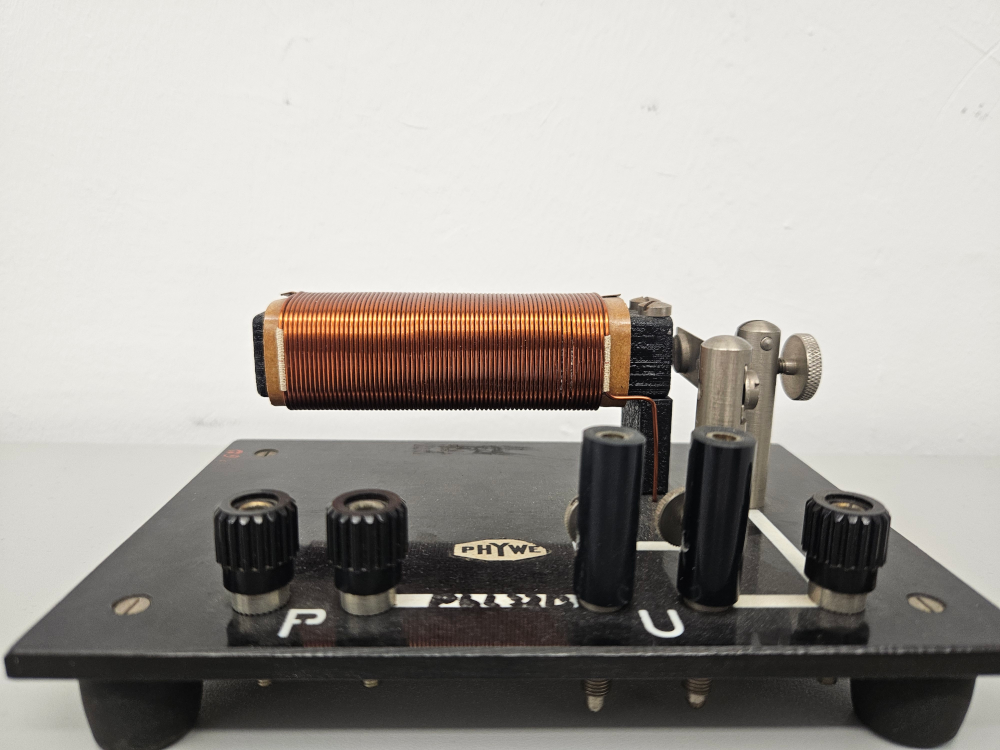
\includegraphics[width=0.75\textwidth]{./Bilder/Spule.png}
        \end{subfigure}%
        \begin{subfigure}{0.45\textwidth}\centering
            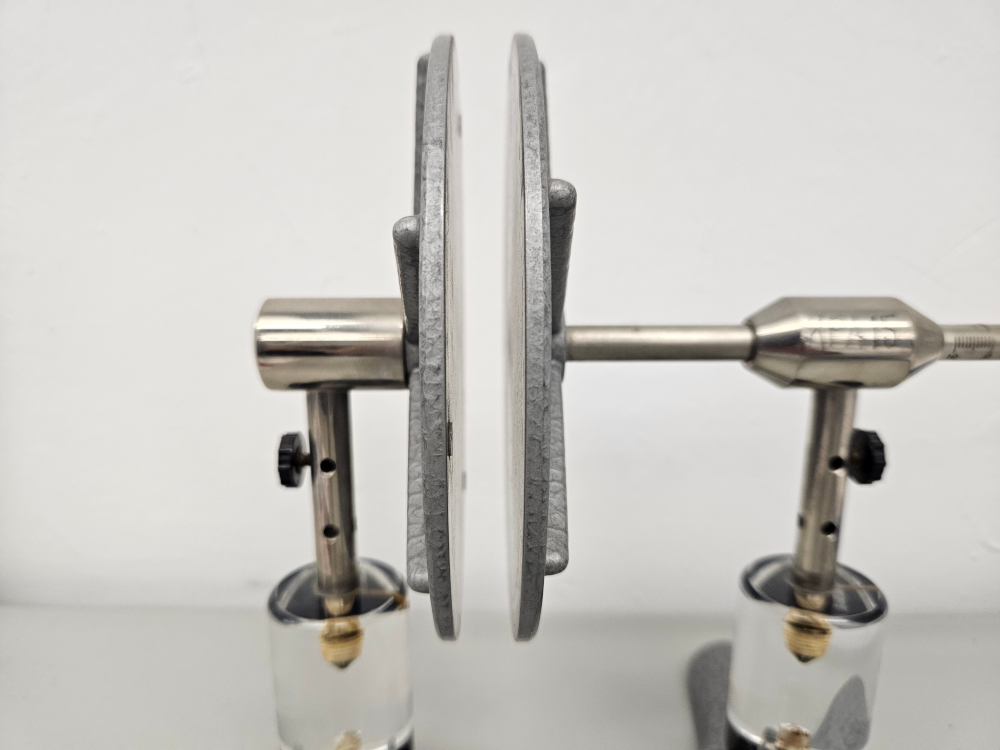
\includegraphics[width=0.75\textwidth]{./Bilder/Kondensator.png}
        \end{subfigure}
        \caption{Reale Induktivät (Spule, links) und Kapazitäten (Kondensator, rechts)}\label{fig:bauteile:realebauteile}
    \end{figure}
    Abbildung \ref{fig:bauteile:realebauteile} zeigt reale Bauteile, die Induktivitäten und Kapazitäten realisieren. 
    Gezeigt sind eine Spule (Induktivität) und ein Kondensator (Kapazität).
}
\b{% Folien-only
\begin{columns}
\column{0.5\textwidth}
    
    \textbf{Induktivität} \begin{tikzpicture}\draw (0,0) to [L,l=$L$] (2,0); \end{tikzpicture}
    \begin{itemize}
%           \item $L = \frac{\Phi}{i}$, mit $\Phi$ als magnetischer Fluss
        \item Impedanz: $\underline{Z}_{\mathrm L} = \mathrm{j}\omega L$
        \item DGL: $\ecv{u_{\mathrm L}} = L \cdot \frac{\d}{\d t}\, \eci{i_{\mathrm L}}$
        \item Energie im Magnetfeld
        \item Ströme stetig (keine Sprünge)
    \end{itemize}

    \textbf{Kapazität} \begin{tikzpicture}\draw (0,0) to [C,l=$C$] (2,0); \end{tikzpicture}
    \begin{itemize}
        \item Impedanz: $\underline{Z}_{\mathrm C} = -\mathrm{j}\frac{1}{\omega C}$
        \item DGL: $\eci{i_{\mathrm C}} = C \cdot \frac{\d}{\d t}\, \ecv{u_{\mathrm C}}$
        \item Energie im elektrischen Feld
        \item Spannungen stetig (keine Sprünge)
    \end{itemize}

% video: 
% nicht überall Sprünge vorgeben können

\column{0.5\textwidth}
    \begin{figure}[H]\centering
        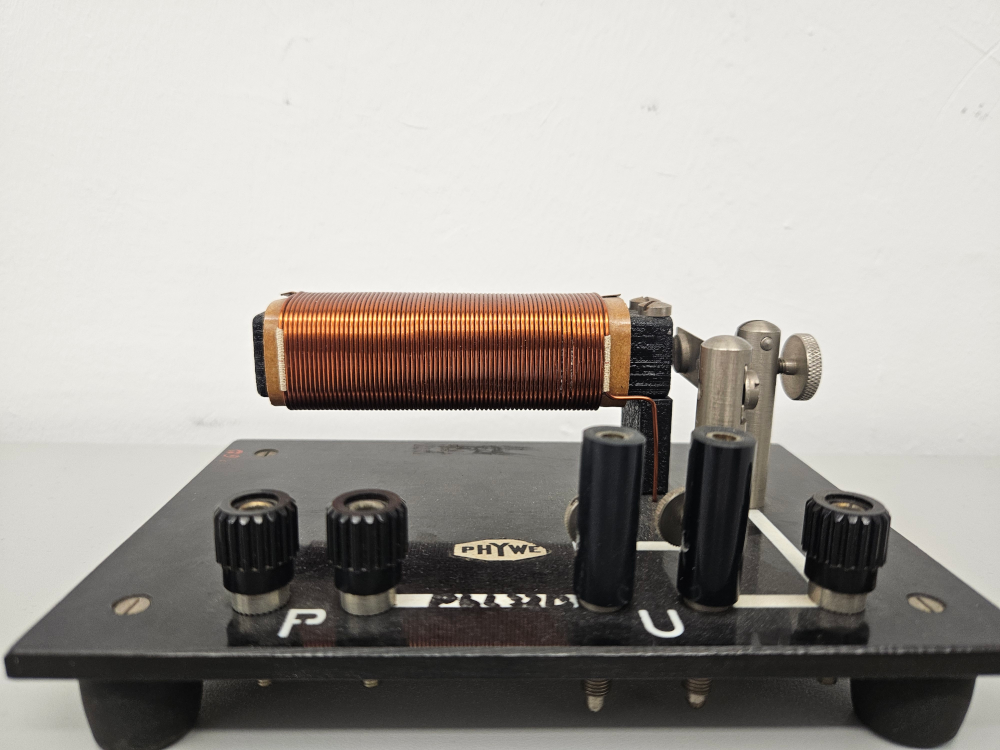
\includegraphics[width=0.5\textwidth]{./Bilder/Spule.png}
        \par Spule
    \end{figure}
    \begin{figure}\centering
        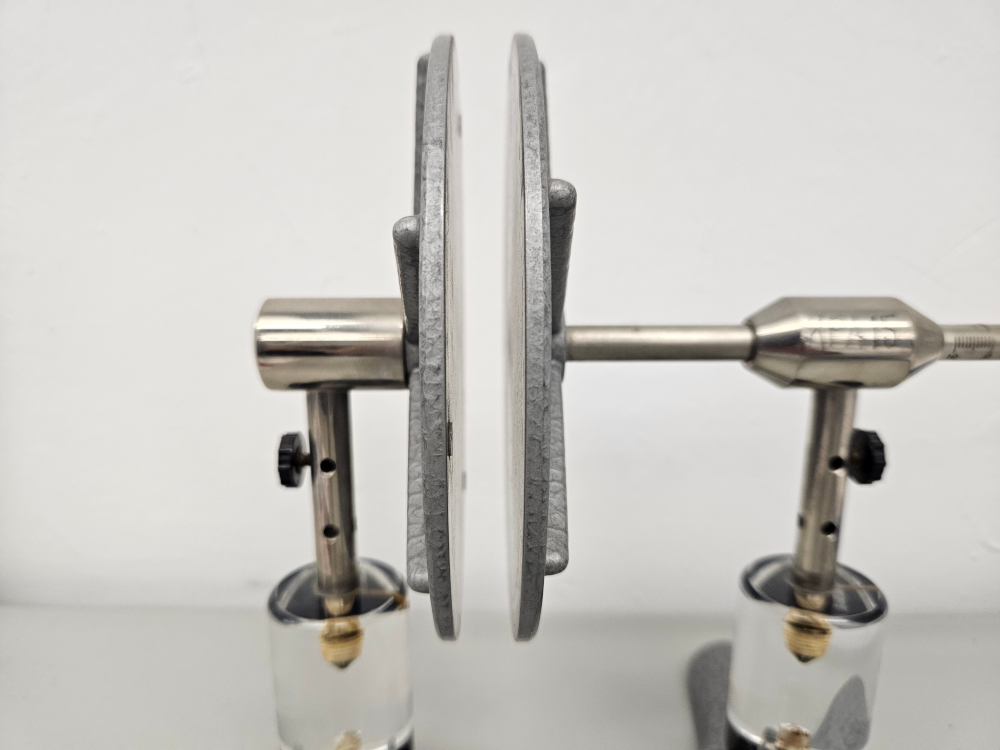
\includegraphics[width=0.5\textwidth]{./Bilder/Kondensator.png}
        %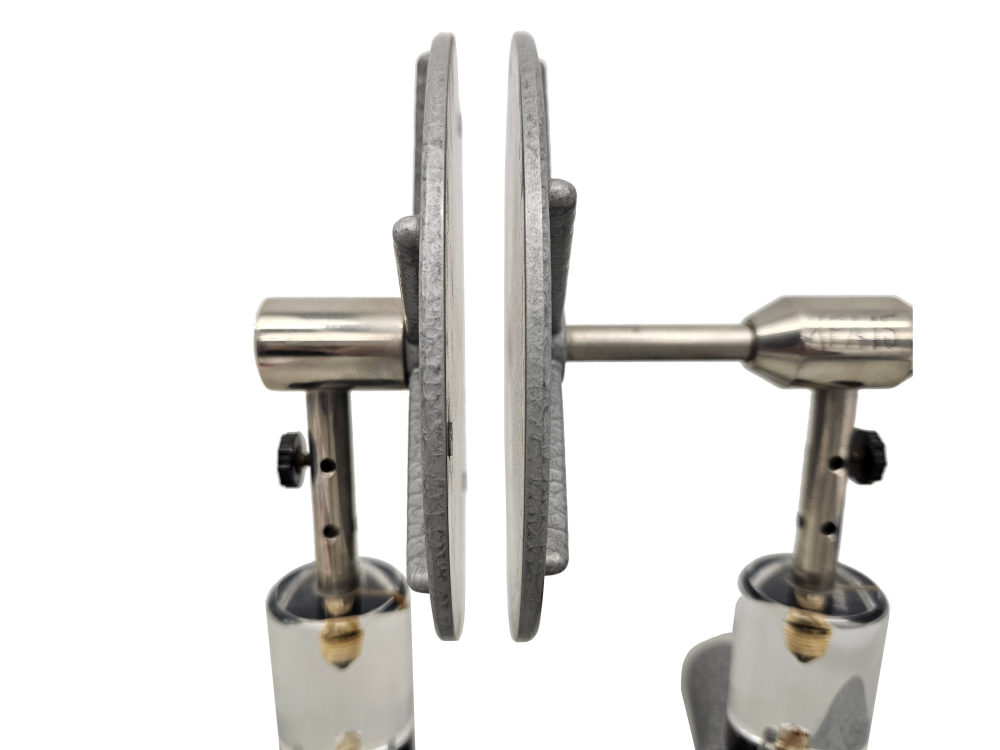
\includegraphics[width=0.5\textwidth]{./Bilder/Kondensator_cut.png}
        \par Kondensator
    \end{figure}
\end{columns}
}% end Folien-only
\end{frame}

%%%%%%%%%%%%%%%%%%%%%%%%%%%%%%%%%%%%%%%%%%%%%%%%%%%%%%%%%%%%%%%%%%%%%%%%%%%%%%%%%%%%%

\subsubsection{Vergleich der linearen Zweipole $R$, $L$ und $C$}
\begin{frame}\ftx{\subsubsecname}

    \s{\ref{tab:vgl:bauteile:rlc} zeigt eine Gegenüberstellung der Größen $R$, $L$ und $C$ und fasst deren wichtigsten Eigenschaften zusammen. }

    % TODO: resizebox für beamer
    % TODO: "Symbol" vertical centering
    % ref: https://tex.stackexchange.com/questions/113022/vertical-alignment-in-tabular-cells-with-variable-height
    % TODO: try \usepackage{tabularx} % column width similar
    \begin{table}[h]\centering%
    \s{\caption{Vergleich lineare Bauteile $R$, $L$, $C$}\label{tab:vgl:bauteile:rlc}}%
    \resizebox{\textwidth}{!}{% for beamer page fit
    \begin{tabular}{ |c|c|c|c|c| }
        \hline &&&&\\[-6pt]
        \textbf{Größe}                          % Col 1
                & \textbf{Allgemein}            % Col 2
                & \textbf{El. Widerstand}       % Col 3
                & \textbf{Induktivität}         % Col 4
                & \textbf{Kapazität} \\[+4pt]   % Col 5
        \hline%
        %\textbf{Symbol}% outcommented, due to no vertical centering
        \begin{tikzpicture}[x=1mm,y=1mm]\draw[draw=none] (-14,-7) rectangle (+14,+7); \node[draw=none,align=center] {\textbf{Symbol}};\end{tikzpicture}
        %\begin{tikzpicture}[x=1mm,y=1mm]\draw[draw=black] (0,0) rectangle (5,5); \draw (2,2) node{S}; % DEBUG WIP 
                % tikzpicture           scaling   \draw     boundbox for same sized pictures    \draw   Bauteil
                & \begin{tikzpicture}[x=1mm,y=1mm]\draw[draw=none] (-14,-7) rectangle (+14,+7); \node[draw=none,align=center] {Zweipol\\Eintor};
                        \draw(0,0) node[dipchip, hide numbers, num pins=4, no topmark, external pins width=0](A){}; % Mittelpunkt des Zweipols
                        \draw(0,0) node[dipchip, hide numbers, num pins=2, no topmark, external pins width=0, opacity=0](B){}; % Ref. Pins mittig
                        \draw(B.bpin 1) to[short,-o] ++(-5,0);
                        \draw(B.bpin 2) to[short,-o] ++(5,0);
                  \end{tikzpicture}
                %& \begin{tikzpicture}[x=1mm,y=1mm]\draw[draw=none] (-4,-5) rectangle (+24,+7);  \draw (5,-5) rectangle (15,5); \draw (10,0) node{Bipol}; 
                %                                                                                \draw (0,0) to [short,o-] (5,0); 
                %                                                                                \draw (15,0) to [short,-o] (20,0); \end{tikzpicture}
                & \begin{tikzpicture}[x=1mm,y=1mm]\draw[draw=none] (-14,-7) rectangle (+14,+7);  \draw (-10,0) to [R,l=$R$,o-o] (10,0); \end{tikzpicture}
                & \begin{tikzpicture}[x=1mm,y=1mm]\draw[draw=none] (-14,-7) rectangle (+14,+7);  \draw (-10,0) to [L,l=$L$,o-o] (10,0); \end{tikzpicture}
                & \begin{tikzpicture}[x=1mm,y=1mm]\draw[draw=none] (-14,-7) rectangle (+14,+7);  \draw (-10,0) to [C,l=$ $,o-o] (10,0); 
                                                                                                \draw (5,3) node{$C$}; \end{tikzpicture} \\[+4pt]
        \hline &&&&\\[-6pt]
        %\textbf{Bauteil}
        %        & Dipol
        %        & Widerstand
        %        & Spule
        %        & Kondensator \\[+4pt]
        %\hline &&&&\\[-6pt]
        \textbf{Einheit}
                & $ \left[\textit{Form.z.}\right] = \mathrm{Einheit} $ 
                & $ \left[R\right] = \Omega\ \text{(Ohm)} $     
                & $ \left[L\right] = \mathrm{H}\ \text{(Henry)} $ 
                & $ \left[C\right] = \mathrm{F}\ \text{(Farad)} $ \\[+4pt]
        \hline &&&&\\[-6pt]
        \textbf{Zeitbereich}
                & $ \frac{\d}{\d t} $ bzw. $ \int \d t $ 
                & $ \ecv{u_{\mathrm{R}}} = R \cdot \eci{i_{\mathrm R}} $     
                & $ \ecv{u_{\mathrm{L}}} = L \cdot \frac{\d}{\d t}\, \eci{i_{\mathrm{L}}} $ 
                & $ \eci{i_{\mathrm{C}}} = C \cdot \frac{\d}{\d t}\, \ecv{u_{\mathrm{C}}} $ \\[+4pt]
        \hline &&&&\\[-6pt]
        \textbf{Frequenzb.}
                & $ \mathrm{j}\omega $ bzw. $ \frac{1}{\mathrm{j}\omega} $
                & $ \ecv{\underline{U}_{\mathrm R}} = R                   \cdot \eci{\underline{I}_{\mathrm R}} $ 
                & $ \ecv{\underline{U}_{\mathrm L}} = \mathrm{j}\omega L  \cdot \eci{\underline{I}_{\mathrm L}} $
                & $ \eci{\underline{I}_{\mathrm C}} = \mathrm{j}\omega C  \cdot \ecv{\underline{U}_{\mathrm C}} $ \\[+4pt]
        \hline &&&&\\[-6pt]
        \textbf{Impedanz}
                & $ \underline{Z} = \frac{\ecv{\underline{U}}}{\eci{\underline{I}}} $
                & $ \underline{Z}_{\mathrm R} = R $ 
                & $ \underline{Z}_{\mathrm L} = \mathrm{j}\omega L $
                & $ \underline{Z}_{\mathrm C} = -\mathrm{j}\frac{1}{\omega C} $ \\[+4pt]
        \hline &&&&\\[-6pt]
        \textbf{Wirkanteil}
                & $ R = \Re\{\underline{Z}\} $
                & $ R = \frac{U}{I} $
                & $ 0 $
                & $ 0 $ \\[+4pt]
                \hline &&&&\\[-6pt]
        \textbf{Blindanteil}
                & $ X = \Im\{\underline{Z}\} $
                & $ 0 $
                & $ X_{\mathrm L} = \omega L $
                & $ X_{\mathrm C} = -\frac{1}{\omega C}$ \\[+4pt]
        \hline
    \end{tabular}
    } % end resizebox
    \end{table}
    
% Für Schaltungen variabler Frequenz: Frequenzvariablen Eigenschaften von Bauteilen, dafür zeitvariante 
\end{frame}

%%%%%%%%%%%%%%%%%%%%%%%%%%%%%%%%%%%%%%%%%%%%%%%%%%%%%%%%%%%%%%%%%%%%%%%%%%%%%%%%%%%

% Beschreibe in Textform wie das Verhalten von Eingangs- zu Ausgangssignalen eines Vierpols 
% mithilfe des Frequenzgangs (bzw. des Amplituden- und Phasengangs) beschrieben werden kann
\s{
\subsection{Zweitore (Vierpole)}
\begin{frame}\ftx{\subsecname}


    % Wiederholung Eintor
    Die Frequenzabhängigkeit von Eintoren (Zweipole) haben wir in Modul 3 bereits untersucht.  
    Mithilfe der komplexen Wechselstromrechnung konnten wir den frequenzabhängigen Wechselstromwiderstand 
    (Impedanz) $\underline{Z}$ einzelner Eintore bestimmen. Durch Anwendung der komplexen Strom- 
    und Spannungsteilerregel konnten wir auch die Gesamt-Impedanz linearer zweipoliger Netzwerke bestimmen. 
    Das heißt für solche, welche nur aus linearen Bauteilen wie $R$, $L$ und $C$ bestehen. 

    % Tikzpicture: Vergleich Vierpol und Zweipol
    %
    % Zeichne links einen senkrechten Zweipol mit Spannungs- (U) und Strompfeil (I) jeweils von oben nach unten
    % Zeichne rechts einen Vierpol (Eingangspole links, Ausgangspole rechts) (U1 links oben nach unten, U2 rechts oben nach unten)
    \begin{figure}[h]
        \begin{subfigure}{0.48\textwidth}\centering
            \includegraphics{Tikz/pdf/circ_eintor.pdf}
        \end{subfigure}\hfill
        \begin{subfigure}{0.48\textwidth}\centering
            \includegraphics{Tikz/pdf/circ_zweitor.pdf}
        \end{subfigure}
        \caption{Vergleich: Schaltzeichen eines allgemeinen Zwei- und Vierpols}
        \label{fig:vgl:zweipolvierpol}
    \end{figure}

    % Einführung Zweitor, wozu
    Zweitore (Vierpole) sind eine Erweiterung von Eintoren (Zweipolen).
    Sie verfügen über eine Eingangs- und eine Ausgangsseite mit jeweiligen Eingangs- und Ausgangsgrößen.  
    Das Zweitormodell eignet sich gut zur Beschreibung von (frequenzabhängigen) Übertragungseigenschaften 
    von elektrischen Netzwerken. 

    \fu{\includegraphics{Tikz/pdf/circ_zweitor_quelle_last.pdf}
    }{Verbindung einer Last über ein Zweitor mit der Quelle.\label{circ:quellezweitorlast}}% im Foliensatz im nächsten Kapitel (Freuqenzgang, Amplitudengang, Phasengang)
    
    Im einfachsten Fall wird wie in \ref{circ:quellezweitorlast} gezeigt, eine Quelle (Eintor) über ein Zweitor 
    mit einer Last (Eintor) verbunden. 
    Typische Zweitore sind beispielsweise Verstärker, Filter oder auch Transformatoren. 
\end{frame}
}% end skript only


    % Wiederholung
\newpage

%%%%%%%%%%%%%%%%%%%%%%%%%%%%%%%%%%%%%%%%%%%%%%%%%%%%%%%%%%%%%%%%%%%%%%%%%%%%%%%%%%%
%%%%%%%%%%%%%%%%%%%%%%%%%%%%%%%%%%%%%%%%%%%%%%%%%%%%%%%%%%%%%%%%%%%%%%%%%%%%%%%%%%%
%                               START KAPITEL 1
%%%%%%%%%%%%%%%%%%%%%%%%%%%%%%%%%%%%%%%%%%%%%%%%%%%%%%%%%%%%%%%%%%%%%%%%%%%%%%%%%%%
%%%%%%%%%%%%%%%%%%%%%%%%%%%%%%%%%%%%%%%%%%%%%%%%%%%%%%%%%%%%%%%%%%%%%%%%%%%%%%%%%%%
\newpage

\section{Frequenzgang, Amplitudengang, Phasengang}
\label{sec:frequenzgang}
\begin{frame}\ftx{\secname}
\s{% Einleitung
    In diesem Kapitel beschäftigen wir uns mit dem Frequenzgang, Amplitudengang und Phasengang von Zweitoren. 
    Diese dienen zur Beschreibung des frequenzvariablen Verhaltens elektrischer Netze in Form von Zweitoren wie in Abbildung \ref{fig:zweitor} gezeigt. 
    Am Beispiel einfacher passiver Filterschaltungen werden wir die Begriffe Frequenz-, Amplituden- und Phasengang einführen und deren Bedeutung und Anwendung erläutern. 

    \fu{\includegraphics{Tikz/pdf/circ_zweitor.pdf}
    }{Schaltsymbol eines Zweitors (Vierpols) mit Eingang (links) und Ausgang (rechts)\label{fig:zweitor}} % in Folien im folgenden Kapitel (Frequenzgang, Amplitudengang, Phasengang)
}%\s Ende
\begin{Lernziele}{Frequenzgang, Amplitudengang, Phasengang}
    Studierende lernen:
    \begin{itemize}
        \item Frequenzgänge anhand der Schaltungstopologie algebreaisch zu bestimmen
        \item die Funktionsweise einfacher Hoch- und Tiefpassfiltern zu verstehen
        \item das Grenzverhalten von Vierpolen anhand ihrer Frequenzgänge zu analysieren
    \end{itemize}
\end{Lernziele}
\end{frame}

\begin{frame}\ftx{\secname}
\b{%
    \begin{minipage}[t][3.5cm][t]{\textwidth}% upper half
        \textbf{Analyse frequenzvariablen Verhaltens elektrischer Netze \only<3->{(Zweitore)}}
        \begin{figure}
            \centering
            \only<beamer:1-2| handout:0>{\includegraphics{Tikz/pdf/circ_zweitor_quelle_last.pdf}}%
            \only<beamer:3-| handout>{\includegraphics{Tikz/pdf/circ_zweitor_longpins.pdf}}%
        \end{figure}%
    \end{minipage}
    \hspace{0.02\linewidth}% for vertical alignment % ref: https://tex.stackexchange.com/questions/378548/vertical-alignment-of-side-by-side-minipages
    \begin{minipage}[c][4cm][c]{0.48\textwidth}% left col
        \only<2>{$\mathrlap{\textbf{Wie sieht das Übertragungsverhalten aus?}}$}%
        \onslide<3->{\textbf{Linear und zeitinvariant (LZI):}}
        \begin{itemize}
            \item<4-> Sinusform am Eingang $u_1(\omega t)$
            \item<5-> $\rightarrow$ Sinusform am Ausgang $u_2(\omega t)$
            \item<5-> $\rightarrow$ Frequenz gleich $\omega_2 = \omega_1$
            \item<6-> $\rightarrow$ Phasenverschiebung $\Delta\varphi = ?$
            \item<6-> $\rightarrow$ Amplitudenverhältnis $\frac{\hat{U}_2}{\hat{U}_1} = ?$
        \end{itemize}
    \end{minipage}
    \hspace{0.02\linewidth}% for vertical alignment
    \begin{minipage}[c][4cm][c]{0.48\textwidth}% right col
        % first plot variant used for beamer and handout, next plot variants only for beamer
        \only<beamer:4|  handout:0>{\includegraphics{Tikz/pdf/plot_sin_comp_amplitude_phase01.pdf}}% If broken slide animations, delete TexAux files and recompile
        \only<beamer:5-6|  handout>{\includegraphics{Tikz/pdf/plot_sin_comp_amplitude_phase02.pdf}}% If broken slide animations, delete TexAux files and recompile
        \only<beamer:7|  handout:0>{\includegraphics{Tikz/pdf/plot_sin_comp_amplitude_phase03.pdf}}% If too long, comment out some of the \only<n>{...} lines
        \only<beamer:8|  handout:0>{\includegraphics{Tikz/pdf/plot_sin_comp_amplitude_phase04.pdf}}% 
        \only<beamer:9| handout:0>{\includegraphics{Tikz/pdf/plot_sin_comp_amplitude_phase05.pdf}}% 
        \only<beamer:10| handout:0>{\includegraphics{Tikz/pdf/plot_sin_comp_amplitude_phase06.pdf}}% 
        \only<beamer:11| handout:0>{\includegraphics{Tikz/pdf/plot_sin_comp_amplitude_phase07.pdf}}% 
        % Currently linear change in amplitude and phase. Could also use "real" change, e.g. Tiefpass behaviour  
    \end{minipage}%
}%
\end{frame}




%%%%%%%%%%%%%%%%%%%%%%%%%%%%%%%%%%%%%%%%%%%%%%%%%%%%%%%%%%%%%%%%%%%%%%%%%%%%%%%%%%%

\subsection[Definitionen]{Definition Frequenzgang, Amplitudengang und Phasengang}
\begin{frame}\ftx{\subsecname}
\begin{columns}[t]
    \column{0.45\textwidth}% left col
        \b{%
            \textbf{Zweitor (Vierpol):}
            \fu{\includegraphics{Tikz/pdf/circ_zweitor.pdf}}{}% im Skript im vorigen Kapitel (Wiederholung)
            \pause%
            \textbf{Linear, zeitinvariant (LZI)}: 
            \begin{equation*}\begin{aligned}
                u_1(t)& = \hat{U}_1 \cdot \sin(\omega t)\\
                \xrightarrow{LZI}\  u_2(t)& = \hat{U}_2 \cdot \sin(\omega t + \varphi)
            \end{aligned}\end{equation*}%  
            \begin{itemize}
                \item[] Sinusform bleibt erhalten
                \item[] Frequenz gleich $\omega_2 = \omega_1$
            \end{itemize}%
        }%
    \column{0.55\textwidth}% right col
        \b{%
        \pause%
            \textbf{Frequenzgang:}%
            \begin{align*}
                \underline{F}(\mathrm{j}\omega) &= \frac{\underline{U}_2}{\underline{U}_1} = A(\omega)\cdot\mathrm e^{\mathrm j\varphi(\omega)}\\[-12pt]% onslide breaks line spacing, manual adjustment
                \onslide<4->{\intertext{\textbf{Amplitudengang:}}%
                A(\omega) &= |\underline{F}(\mathrm{j}\omega)| = \frac{|\underline{U}_2|}{|\underline{U}_1|}\\
                &= \sqrt{\left(\Re\{\underline{F}(\mathrm{j}\omega)\}\right)^2 + \left(\Im\{\underline{F}(\mathrm{j}\omega)\}\right)^2}\\[-12pt]% onslide breaks line spacing, manual adjustment
                }% end onslide
                \onslide<5->{\intertext{\textbf{Phasengang:}}%
                \varphi(\omega) &= \angle \underline{F}(\mathrm{j}\omega) = \angle \underline{U}_2 - \angle \underline{U}_1\\
                &= \arctan\left(\frac{\Im\{\underline{F}(\mathrm{j}\omega)\}}{\Re\{\underline{F}(\mathrm{j}\omega)\}}\right)%
                }% end onslide
            \end{align*}
        }%
        \s{%
            % Definition Frequenzgang
            \index{Frequenzgang}%
            \index{lineares zeitinvariantes System}%
            Der \textbf{Frequenzgang} $\underline{F}(\mathrm{j}\omega)$, auch komplexer Amplitudengang genannt, 
            beschreibt das Verhältnis von Ausgangs- zu Eingangssignal eines linearen zeitinvarainten Systems (LZI-System) bei sinusförmiger Anregung.
            Er bietet eine Möglichkeit frequenzabhängiges Verhalten von Zweitoren zu untersuchen, 
            ist ein Spezialfall der Laplace-Übertragungsfunktion aus der Systemtheorie und 
            wird wie folgt definiert:

            \begin{equation}
                \underline{F}(\mathrm{j}\omega) = \frac{\underline{U}_2}{\underline{U}_1}% F(jw)=U2/U1
                \label{eq:def:F}
            \end{equation}

            % Amplituden und Phasenänderung
            \index{Amplitudengang}%
            \index{Phasengang}%
            Aufgrund der Linearität von LZI-Systemen bleiben Frequenz und Sinusform am Ausgang erhalten. 
            Amplitude und Phase können sich in Abhängigkeit der Frequenz vom Eingang zum Ausgang ändern. 
            Erkennbar ist dies insbesondere in der Schreibweise in Polarkoordinaten. 

            \begin{equation}
                \underline{F}(\mathrm{j}\omega) = A(\omega)\cdot\mathrm e^{\mathrm j\varphi(\omega)}% F(jw)=A*exp(jphi)
                \label{eq:def:Fpolar}
            \end{equation}
            Der \textbf{Amplitudengang} $A(\omega)$ beschreibt die relative Amplitudenänderung 
            zwischen Aus- und Eingangsspannung und entspricht dem Betrag des Frequenzganges.
            Der \textbf{Phasengang} $\varphi(\omega)$ hingegen, beschreibt die absolute Phasenänderung
            zwischen Aus- und Eingangsspannung und entspricht der Phase des Frequenzganges.
            Über $\underline{F}(\mathrm{j}\omega)$ können wir beide wie folgt definieren: 

            \begin{align}
                \label{eq:def:A}
                A(\omega)       & = |\underline{F}(\mathrm{j}\omega)|&
                                & = \sqrt{\left(\Re\{\underline{F}(\mathrm{j}\omega)\}\right)^2 + \left(\Im\{\underline{F}(\mathrm{j}\omega)\}\right)^2}&
                                & = \frac{|\underline{U}_2|}{|\underline{U}_1|}\\
                \label{eq:def:phi}
                \varphi(\omega) & = \angle \underline{F}(\mathrm{j}\omega)&
                                & = \arctan\left(\frac{\Im\{\underline{F}(\mathrm{j}\omega)\}}{\Re\{\underline{F}(\mathrm{j}\omega)\}}\right)&
                                & = \angle \underline{U}_2 - \angle \underline{U}_1
            \end{align}
        }
% Hinweis: Spannungsbezug Regel, Strombezug nicht betrachtet 
%Der Frequenzgang bezieht sich in der Regel auf Spannungen, nicht auf Ströme, da in der Regel Spannungs- 
%statt Stromquellen verwendet werden. In diesem Skript bezieht sich der Frequenzgang daher immer auf Spannungen.
\end{columns}
\end{frame}

%%%%%%%%%%%%%%%%%%%%%%%%%%%%%%%%%%%%%%%%%%%%%%%%%%%%%%%%%%%%%%%%%%%%%%%%%%%%%%%%%%%

\subsection{Frequenzgang am Beispiel eines einfachen Tiefpass-Filters}
\label{sec:frequenzgang:tiefpass:herleitung}
\begin{frame}[t]\ftx{\subsecname}
\begin{columns}[T]%
\column{0.45\textwidth}% left col
    \s{\index{Filter>Tiefpass}%
        Das Zweitor in Abbildung \ref{circ:filter:rctief} stellt einen einfachen Tiefpass-Filter (kurz Tiefpass) dar.
        Der Name Tiefpass leitet sich von dem Verhalten her, dass Signale tiefer Frequenzen nahezu unverändert passieren,
        Signale hoher Frequenzen jedoch stark gedämpft (gefiltert) werden.
        Die Funktionsweise und das Verhalten des Tiefpasses lassen sich gut mittels einer Frequenzganganalyse veranschaulichen.

        \fu{\includegraphics{Tikz/pdf/circ_tiefpass_rc_annotated.pdf}}{Schaltbild, RC-Tiefpass 1. Ordnung\label{circ:filter:rctief}}%

        Der gezeigte Tiefpass besteht aus einer Serienschaltung aus $R$ und $C$ mit Eingangsspannung $\underline{U}_1$
        über beiden Elementen und Ausgangsspannung $\underline{U}_2$ über $C$.
        Da die Einzelelemente $R$ und $C$ lineare, zeitinvariante (LZI-)Bauteile sind, 
        ist auch der daraus zusammen gesetzte Tiefpass ein LZI-System.
        Das bedeutet, dass bei Anregung der Schaltung mit einer sinusförmigen Eingangsspannung $u_1(t)$ (links),
        die Ausgangsspannung $u_2(t)$ (rechts) ebenfalls sinusförmig ist und die gleiche Frequenz besitzt wie die Eingangsspannung.
    }%
    \b{%
    {\centering
    \vspace{-7.5mm}%
    \onslide<1->{\includegraphics{Tikz/pdf/circ_tiefpass_rc_annotated.pdf}}%
    }\vspace{3mm}%
        
    \textbf{RC-Tiefpass 1. Ordnung}
    \begin{equation*}\begin{aligned}
            u_1(t)& = \hat{U}_1 \cdot \sin(\omega t)\\\xrightarrow{LZI}\ 
            u_2(t)& = \hat{U}_2 \cdot \sin(\omega t + \varphi)
        \end{aligned}\end{equation*}%
    \pause%
    }
\column{0.55\textwidth}% right col
    \s{%
        \begin{equation}\begin{aligned}
            u_1(t)& = \hat{U}_1 \cdot \sin(\omega t)\\\xrightarrow{LZI}\ 
            u_2(t)& = \hat{U}_2 \cdot \sin(\omega t + \varphi)
        \end{aligned}\end{equation}%
        Die LZI-Eigenschaft ist Voraussetzung zur Bestimmung des Frequenzganges und die Anwendung der komplexen Wechselstromrechnung.
        Zusätzliche Voraussetzung ist die Annahme einer sinusförmigen Anregung im eingeschwungenen Zustand, von der wir zwecks Analyse ausgehen.
        Statt der Ein- und Ausgangsspannung $u_1(t)$ und $u_2(t)$ im Zeitbereich betrachten wir die entsprechende
        komplexe Ein- und Ausgangsspannung $\underline{U}_1$ und $\underline{U}_2$ im Frequenzbereich wie im Schaltbild dargestellt.

        Der Frequenzgang $\underline{F}(\mathrm{j}\omega)$ entspricht nach Gleichung \ref{eq:def:F} 
        dem komplexen Spannungsverhältnis von Ausgangs- zu Eingangsspannung $\underline{U}_2/\underline{U}_1$.
        Gemäß komplexer Spannungsteilerregel entspricht das Spannungsverhältnis dem Verhältnis der Impedanz am Ausgang (Impedanz der Kapazität) und 
        der Impedanz am Eingang (Summe der Impedanz von Kapazität und Widerstand), kurz $\frac{\underline{Z}_C}{R + \underline{Z}_C}$.

        Gleichung \ref{eq:tiefpass:frequenzgang} zeigt den ermittelten Frequenzgang des Tiefpasses.
        Zur Vereinfachung wurden Nenner und Zähler rationalisiert, der Nenner sortiert und der Term
        (optional) in kartesische Koordinaten umgeformt. (Vergleich kommentierte Nebenrechnung \ref{eq:tiefpass:frequenzgang:nebenrechnung}):
    }%
    \b{%
        \textbf{Frequenzgang:}%
        \begin{align*}% lesser space above than \begin{equation}\begin{align} ... as in skript version below
            \underline{F}(\mathrm{j}\omega)   & = \frac{\underline{U}_2}{\underline{U}_1} 
                                    = \frac{\frac{1}{\mathrm{j}\omega C}}{R + \frac{1}{\mathrm{j}\omega C}}
                                    = \frac{1}{\mathrm{j}\omega CR + 1} \\
                                    & = \frac{1}{1 + \mathrm{j}\omega CR}
                                    = \frac{1 - \mathrm{j}\omega CR}{1 + (\omega CR)^2}
        \end{align*}%
        \pause%
    }%
    \s{%
        \begin{equation}
            \begin{aligned}
                \underline{F}(\mathrm{j}\omega)   & = \frac{\underline{U}_2}{\underline{U}_1}
                                        = \frac{\frac{1}{\mathrm{j}\omega C}}{R + \frac{1}{\mathrm{j}\omega C}}
                                        = \frac{1}{\mathrm{j}\omega CR + 1} \\
                                        & = \frac{1}{1 + \mathrm{j}\omega CR}
                                        = \frac{1 - \mathrm{j}\omega CR}{1 + (\omega CR)^2}
            \end{aligned}\label{eq:tiefpass:frequenzgang}
        \end{equation}
    }%

    \s{
        Damit haben wir den $\underline{F}(\mathrm{j}\omega)$ in Abhängigkeit von $\omega$ 
        und den Bauteilgrößen $C$ und $R$ ermittelt. 
        Mittels Betragsbildung lässt sich daraus gemäß \eqref{eq:def:A} der Amplitudengang 
        und durch Phasenberechnung gemäß \eqref{eq:def:phi} der Phasengang bestimmen.
        
        Zur Betragsbildung bietet sich die Form $\frac{1}{1+\mathrm{j}\omega CR}$ an.
        Da der Betrag im Zähler direkt ablesbar $1$ beträgt, muss nur der Betrag im Nenner 
        bestimmen werden wie sie in \eqref{eq:tiefpass:ampli} gezeigt ist.
        Alternativ kann auch die kartesische Form aus \eqref{eq:tiefpass:frequenzgang} in 
        \eqref{eq:def:A} eingesetzt werden. 

        Für den Phasengang $\varphi(\omega)$ bietet sich die kartesische Schreibweise in 
        der Form $\frac{1-\mathrm{j}\omega CR}{1+(\omega CR)^2}$ an.
        In dieser lassen sich der Real- und Imaginärteil leicht ablesen. 
        Der Nenner hat dabei als rein reelle Größe keinen Einfluss auf die Phasenlage 
        wie in \eqref{eq:tiefpass:phase} gezeigt ist.
    }%
    
    \b{\textbf{Amplituden- und Phasengang:}
        \begin{align*}
            A(\omega)       &= |\underline{F}(\mathrm{j}\omega)| = \frac{|\underline{U}_2|}{|\underline{U}_1|}
                            &= \frac{1}{\sqrt{1 + (\omega CR)^2}} \\%
            \varphi(\omega) &= \arctan\left(\frac{\Im\{\underline{F}\}}{\Re\{\underline{F}\}}\right)
                            &= \arctan\left(-\omega CR\right)        
        \end{align*}
    }
    \s{% Ohne Überschrift, Rechnung etwas ausführlicher
        \begin{align}
            A(\omega)       &= |\underline{F}(\mathrm{j}\omega)| = \left|\frac{1}{1+\mathrm{j}\omega CR}\right|
                                &&= \frac{\left|\qquad\!1\!\qquad\right|}{\left|1+\mathrm{j}\omega CR\right|} % Extra step
                            &= \frac{1}{\sqrt{1 + (\omega CR)^2}} \label{eq:tiefpass:ampli}\\
            \varphi(\omega) &= \angle \underline{F}(\mathrm{j}\omega) = \angle\left(\frac{1 - \mathrm{j}\omega CR}{\redcancel{1+(\omega CR)^2}}\right)
                                &&= \arctan\left( \dfrac{ \dfrac{-\omega CR}{\redcancel{1+(\omega CR)^2}} }{ \dfrac{1}{\redcancel{1+(\omega CR)^2}} } \right) % Extra step
                            &= \arctan\left(-\omega CR\right) \label{eq:tiefpass:phase}
        \end{align}

        Alternativ kann der Phasengang auch aus der nicht kartesischen Form des Frequenzganges bestimmt werden. 
        Der Phasengang ergibt sich aus der Phasenlage des Zählers subtrahiert mit der Phasenlage des Nenners: 
        
        \begin{align}
            \varphi(\omega) 
            &= \angle \left(\frac{1}{1+\mathrm{j}\omega CR}\right) 
            = \underbrace{\arctan\left(\frac{0}{\redcancel{1}}\right)}_{\varphi_{Zaehler}}-\underbrace{\arctan\left(\frac{\omega CR}{\redcancel{1}}\right)}_{\varphi_{Nenner}}
            &= \arctan\left(-\omega CR\right) \label{eq:tiefpass:phase:alternative}
        \end{align}

        Die Herangehensweise bietet sich vor allem an, wenn sich Betrag und/oder Phase des Zählers direkt ablesen lassen. 
        Dadurch kann ein Rechenschritt zum Umrechnen in kartesische Koordinaten gespaart werden.

        Im folgenden Exkurs wird die seperate Betrachtung von Zähler und Nenner von Frequenzgängen näher erläutert:

        \textbf{Exkurs Berechnung komplexer Zahlen in (kartesischen) Descartes- und Polar-Koordinaten}

        Der Frequenzgang nimmt in der Regel die Form eines komplexen gebrochen rationalen Bruches an. 
        Das bedeutet, dass sowohl Nenner als auch Zähler sich als komplexe Polynome darstellen lassen:
        
        \begin{equation}
            \label{eq:def:F:komplexgebrochenrationalerbruch}
            \underline{F}(\mathrm{j}\omega) 
                = \frac{\underline{F}_Z(\mathrm{j}\omega)}{\underline{F}_N(\mathrm{j}\omega)}
                = \frac{a_n \omega^n + \dots + a_1 \omega + a_0}{b_m \omega^m + \dots + b_1 \omega + b_0} \qquad \text{mit} 
                \qquad a_i, b_j \in \mathbb{C} 
                \qquad n,m,\omega \in \mathbb{R} 
                %\qquad i \in \left[0,...,n\right] 
                %\qquad j \in \left[0,...,m\right]
        \end{equation}
        
        Liegt $\underline{F}(\mathrm{j}\omega)$ nun als komplexer Bruch vor mit Zähler und Nenner in kartesischen Koordinaten, 
        so können wir $A(\omega)$ und $\varphi(\omega)$ durch seperate Betragsbildung und Phasenberechnung von Zähler und Nenner bestimmen.
        Hierfür werden die Formeln aus \eqref{eq:def:A} und \eqref{eq:def:phi} für Zähler (Index $Z$) und Nenner (Index $N$) angewandt. 
        Da Amplituden- und der Phasengang wie in \eqref{eq:def:Fpolar} gezeigt die Polar-Koordinaten (Amplitude und Phase) des Frequenzganges 
        darstellen ergibt sich folgendes Berechnungsschema:

        \begin{align}
            \label{eq:def:F:bruch}
            \underline{F}(\mathrm{j}\omega) 
                            & = \frac{\underline{F}_Z(\mathrm{j}\omega)}{\underline{F}_N(\mathrm{j}\omega)}&
                            & = \frac{|\underline{F}_Z| \cdot \mathrm{e}^{\mathrm{j}\angle{\underline{F}_Z}}}{|\underline{F}_N| \cdot \mathrm{e}^{\mathrm{j}\angle{\underline{F}_N}}}&
                            & = \frac{A_Z}{A_N} \cdot \mathrm{e}^{\mathrm{j} (\varphi_Z - \varphi_N)}
                            \vphantom{\Bigg|}\\
            \label{eq:def:A:bruch}
            A(\omega)       & = |\underline{F}(\mathrm{j}\omega)|&
                            & = \frac{|\underline{F}_Z|}{|\underline{F}_N|}&
                            & = \frac{A_Z}{A_N}&
                            \vphantom{\Bigg|}\\
            \label{eq:def:phi:bruch}
            \varphi(\omega) & = \angle \underline{F}(\mathrm{j}\omega)&
                            & = \angle{\underline{F}_Z} - \angle{\underline{F}_N}&
                            & = \varphi_Z - \varphi_N
        \end{align}

        Im Allgemeinen bietet sich für Multiplikationen und Divisionen komplexer Zahlen die Berechnung in Polarkoordinaten (mit Betrag und Argument) an.
        Eine Multiplikation/Division führt bei komplexen Zahlen zur Multiplikation/Division der Beträge und Addition/Subtraktion der Argumente.
        Bei Additionen und Subtraktionen eignet sich die kartesische Form mit Real- und Imaginärteil besser für Berechnungen, 
        da diese direkt addiert/subtrahiert werden können.
    }
\end{columns}
    \CMT{% COMMENT ANFANG
    \begin{align}
        \underline{z}   
        &= \Re\{\underline{z}\} + \mathrm{j} \Im\{\underline{z}\}  &
            &= x + \mathrm{j}y &
            &\text{mit}\quad x,y \in \mathbb{R} \\
        &= |\underline{z}|\cdot \mathrm{e}^{\mathrm{j}\angle{\underline{z}}} &
            &= a \cdot \mathrm{e}^{\mathrm{j} \beta} &
            &\text{mit}\quad a,\beta \in \mathbb{R}\\
    \end{align}
    }% COMMENT ENDE
\end{frame}

%%%%%%%%%%%%%%%%%%%%%%%%%%%%%%%%%%%%%%%%%%%%%%%%%%%%%%%%%%%%%%%%%%%%%%%%%%%%%%%%%%%

\subsection{Grenzverhalten am Beispiel eines einfachen Tiefpass-Filters}
\label{sec:frequenzgang:tiefpass:grenzverhalten}
\begin{frame}[t]\ftx{\subsecname}
\b{
    \begin{columns}[T]
        \column{0.45\textwidth}% column links 1/2
            {\centering%
            \vspace{-7.5mm}%
            \onslide<1->{\includegraphics{Tikz/pdf/circ_tiefpass_rc_annotated.pdf}}%
            \vspace{2mm}%

            \onslide<6->{\resizebox{\textwidth}{!}{\includegraphics{Tikz/pdf/plot_tiefpass_mini_ampli_lin_samesize.pdf}}}

            \onslide<6->{\resizebox{\textwidth}{!}{\includegraphics{Tikz/pdf/plot_tiefpass_mini_phase_lin_samesize.pdf}}}
            }%
        \column{0.55\textwidth}% column rechts 2/2
            \b{\textbf{Grenzverhalten:} für $f \rightarrow 0$ und $f \rightarrow \infty$\\[-12pt]%
            }%
            % Rechnung
            \begin{align*}
                \onslide<1->{\underline{F}(\mathrm{j}\omega)&=A(\omega)\cdot\mathrm e^{\mathrm j\varphi(\omega)} = \frac{1}{1 + \mathrm{j}\omega CR} &&}\\[+8pt] % extra space
                \onslide<2->{A(\omega)      &=\frac{1}{\sqrt{1 + (\omega CR)^2}}                                    &&\\}%
                \onslide<3->{%
                                            &\lim_{\omega \rightarrow 0}A(\omega) = \frac{1}{1}                     &&=1\\
                                            &\lim_{\omega \rightarrow \infty}A(\omega) = \frac{1}{\sqrt{\infty}}    &&=0\\[+8pt] % extra space
                }%
                \onslide<4->{\varphi(\omega)&=\arctan\left(-\omega CR\right)                                        &&\\}%
                \onslide<5->{%
                                            &\lim_{\omega \rightarrow 0}         \varphi(\omega) = \arctan(0)       &&=0\degree\\
                                            &\lim_{\omega \rightarrow \infty}    \varphi(\omega) = \arctan(-\infty) &&=-90\degree
                }%   
            \end{align*}
    \end{columns}
}
\s{
    In diesem Kapitel wird das Grenzverhalten des Tiefpass-Filters 1. Ordnung aus dem vorigen Kapitel (s. Abbildung \ref{circ:filter:rctief}) für sehr hohe und sehr niedrige Frequenzen untersucht.
    Dazu werden die Grenzwerte des Amplitudengangs $A(\omega)$ und des Phasengangs $\varphi(\omega)$ bestimmt, sowie die Ergebnisse beschrieben, interpretiert und grafisch dargestellt.
    
    \textbf{Grenzwerte:}

    Für den Amplitudengang aus Gleichung \ref{eq:tiefpass:ampli} ergeben sich
    für $f \rightarrow 0$ und $f \rightarrow \infty$ die folgenden Grenzwerte:

    \begin{align}
        &&A(\omega) &=\frac{1}{\sqrt{1 + (\omega CR)^2}}    &                                           &                           &   &    &&\nonumber\\
        &&          &                                       &   \lim_{\omega \rightarrow 0}A(\omega)    &=\frac{1}{1}               &   &=1  &&\label{eq:tiefpass:ampli:lim}\\
        &&          &                                       &   \lim_{\omega \rightarrow \infty}A(\omega)&=\frac{1}{\sqrt{\infty}}  &   &=0  &&\nonumber
    \end{align}
    %\\\intertext{%
    %    Für den Phasengang aus Gleichung \ref{eq:tiefpass:phase} ergeben sich analog dazu die Grenzwerte:%
    %}%
    Für den Phasengang aus Gleichung \ref{eq:tiefpass:phase} ergeben sich analog dazu die Grenzwerte:
    \begin{align}
        &&\varphi(\omega)   &=\arctan\left(-\omega CR\right)&                                                   &                   &   &           &&\nonumber\\
        &&                  &                               &   \lim_{\omega \rightarrow 0}\varphi(\omega)      &=\arctan(0)        &   &=0\degree  &&\label{eq:tiefpass:phase:lim}\\
        &&                  &                               &   \lim_{\omega \rightarrow \infty}\varphi(\omega) &=\arctan(-\infty)  &   &=-90\degree&&\nonumber
    \end{align}

    An Gleichung \ref{eq:tiefpass:ampli:lim} ist zu erkennen, dass der Tiefpass bei sehr niedrigen Frequenzen kaum dämpft ($A(\omega) \rightarrow 1$), 
    bei sehr hohen Frequenzen hingegen stark dämpft ($A(\omega) \rightarrow 0$). 
    
    An Gleichung \ref{eq:tiefpass:phase:lim} ist zu erkennen, dass der Tiefpass bei sehr niedrigen Frequenzen (bei kaum Dämpfung) kaum Phasenverschiebung aufweist ($\varphi(\omega) \rightarrow 0\degree$),
    bei sehr hohen Frequenzen (starke Dämpfung) hingegen eine Phasenverschiebung bis $-90\degree$ aufweist. 

    \textbf{Erklärung des Grenzverhaltens anhand des Schaltbildes:}

    Das Grenzverhalten bezüglich Amplitudenänderung und Phasenverschiebung lässt sich gut anhand des 
    Schaltbildes \ref{circ:filter:rctief} erklären. % TODO: Schaltbilder für Grenzfälle mit Spannungspfeilen und Impedanzen einfügen
    
    Im Grenzfall einer Gleichspannung ($f=0$) am Eingang sperrt die Kapazität ($X_C \rightarrow \infty$). 
    Ihr Verhalten entspricht hier zwei offenen Klemmen, wodurch die gesamte Eingangsspannung am Ausgang $U_2$ über der Kapazität $C$ anliegt. 
    Die relative Amplitudenänderung beträgt daher $1$ (ungedämpft) und die Phasenverschiebung $0\degree$ (in Phase). 

    Bei sehr hohen Frequenzen ($f\rightarrow \infty$) verhält sich die Kapazität wie ein Kurzschluss ($X_C \rightarrow 0$).
    Damit geht die Ausgangsspannung gegen null (starke Dämpfung, $A\rightarrow 0$) und die Eingangsspannung liegt annäherend vollständig über $R$ an.
    Eingangsspannung und Strom liegen dadurch näherungsweise in Phase. Die Phasenverschiebung von Ausgangsspannug über der Kapazität
    zu Eingangsspannung beträgt dadurch näherungsweise $-90\degree$.
    
    \textbf{Visualisierung:}

    % Hinweis zur Visualisierung der Funktionen
    Um eine Vorstellung des Verhaltens von Amplituden- und Phasengang zu bekommen, können wir die Funktionen graphisch darstellen. 

    Der Amplitudengang $A(\omega)$ und der Phasengang $\varphi(\omega)$ sind in 
    Abbildung \ref{plot:tiefpass:ampli:mini:lin} und \ref{plot:tiefpass:phase:mini:lin} dargestellt.
    Beide Graphen sind mit linearen Skalen dargestellt, wobei die Skalierungen beider x-Achsen für $\omega \left[\mathrm{Hz}\right]$ identisch sind. 
    Eine Veränderung des Faktors $CR$ führt in linearer Darstellung lediglich zu einer Stauchung oder Streckung der Graphen in x-Richtung, 
    weshalb auf eine explizite Angabe der Werte verzichtet wurde. 

    \begin{figure}[h]\centering
        \begin{subfigure}{0.45\textwidth}\centering
            \includegraphics{Tikz/pdf/plot_tiefpass_mini_ampli_lin_samesize.pdf}
            \caption{Amplitudengang $A(\omega)$, lineare Achsen}
            \label{plot:tiefpass:ampli:mini:lin}
        \end{subfigure}
        \begin{subfigure}{0.45\textwidth}\centering
        \includegraphics{Tikz/pdf/plot_tiefpass_mini_phase_lin_samesize.pdf}
            \caption{Phasengang $\varphi(\omega)$, lineare Achsen}
            \label{plot:tiefpass:phase:mini:lin}
        \end{subfigure}
        \caption{Lineardarstellung des Amplitudengang und Phasengang eines Tiefpass 1. Ordnung}
%        \caption{Amplitudengang $A(\omega)$ und Phasengang $\varphi(\omega)$ eines Tiefpass 1. Ordnung, lineare Achsen}
        \label{plot:tiefpass:mini:lin}
    \end{figure}

    % Hinweis: Logarithmische Skala für Frequenzgang
    In Kapitel \ref{sec:frequenzganglog} wird die Darstellung des Frequenzganges mit logarithmischer Skala eingeführt.
    Auch die Definition der \textbf{Grenzfrequenz} $f_g$ (respektive der Grenzkreisfrequenz $\omega_g$) zur Unterteilung 
    des Frequenzbereichs in einen \textbf{Durchlassbereich} und einen \textbf{Sperrbereich} wird dort erläutert.

    \textbf{Exkurs zur Herleitung der Graphenform:}
    % Erklärung der Graphenform für A(omega) anhand von Näherungen (Potenzfunktion)

    Die Graphenform des Amplitudengangs $A(\omega)$  in linearer Darstellung lässt sich daran erklären, dass dieser sich 
    für sehr niedrige Frequenzen ($f \rightarrow 0$) der waagrechten Gerade $A=1$ annähert und 
    für sehr hohe Frequenzen ($f \rightarrow \infty$) der Potenzfunktion $\frac{1}{\omega CR}$ annähert.
    Abbildung \ref{plot:tiefpass:ampli:lin:approx} zeigt diese Näherungen für $A(x)=\frac{1}{\sqrt{1+x^2}}$ mit $x=\omega CR$.

    \fu{\includegraphics{Tikz/pdf/plot_tiefpass_ampli_lin_approx.pdf}}{
        Amplitudengang Tiefpass 1. Ordnung, lineare Achsen, Näherungen mit $x=\omega CR$ \label{plot:tiefpass:ampli:lin:approx}
    }

    % Erklärung der Graphenform für phi(omega) anhand von Tangensfunktion
    Die Form des Phasenganges lässt sich leicht aus der Form einer (Arcus-)Tangensfunktion ableiten.
    Abbildung \ref{plot:tiefpass:phase:lin:approx} zeigt die Tangensfunktion und dessen Umkehrfunktion Arcustangens, sowie deren 
    jeweiligen Spiegelungen an der y-Achse in linearer Darstellung.
    
    \fu{\includegraphics{Tikz/pdf/plot_tan_atan_mirror.pdf}}{
        Phasengang Tiefpass 1. Ordnung, lineare Achsen, Vergleich Tangens/Arcustangens \label{plot:tiefpass:phase:lin:approx}
    }

    Die Umkehrung der jeweiligen Funktion ist durch Spiegelung des Graphen an der Winkelhalbierenden 
    (schwarz gestrichelte Gerade) und Tausch der x- und y-Achse erreichbar,
    vorrausgesetzt die jeweilige Funktion ist stetig monoton wachsend oder stetig monoton fallend. 
    Der Tangens ist daher zur Bildung des Arcustangens auf den Winkelbereich $-90\degree$ bis $+90\degree$ beschränkt 
    bei einem Wertebereich von $-\infty$ bis $+\infty$.
    Aufgrund der nicht darstellbaren Polstellen ist der dargestellte Wertebereich auf $-6$ bis $+6$ beschränkt.

    Der Phasengang des Tiefpass 1. Ordnung entspricht dem abgebildeten $\arctan(-x)$ für $x=\omega CR >0$. 
    Da es physikalisch keine negativen Frequenzen gibt, gilt $\omega>0 \rightarrow x>0$, wodurch der Wertebereich des Phasengangs 
    nur den halben Wertebereich des Arcustangens abdeckt, also von $-90\degree$ bis $0\degree$.
}%
\end{frame}

%%%%%%%%%%%%%%%%%%%%%%%%%%%%%%%%%%%%%%%%%%%%%%%%%%%%%%%%%%%%%%%%%%%%%%%%%%%%%%%%%%%

\subsection{Frequenzgang am Beispiel eines einfachen Hochpass-Filters}
\label{sec:frequenzgang:hochpass:herleitung}
\begin{frame}\ftx{\subsecname}
    \begin{columns}
        \column[T]{0.45\textwidth}% left col
            \s{\index{Filter>Hochpass}%
                Ein Hochpass-Filter (kurz Hochpass) funktioniert ähnlich einem Tiefpass-Filter. 
                Dem Namen entsprechend passieren beim Hochpass jedoch Signale hoher Frequenzen nahezu ungedämpft (ungefiltert), 
                während Signale niedriger Frequenzen stark gedämpft (gefiltert) werden.  

                % Aufbau (Schaltbild)
                Abbildung \ref{circ:filter:rchoch} zeigt exemplarisch einen RC-Hochpass erster Ordnung, 
                der im Folgenden näher untersucht wird.
                Der Hochpass besteht aus einer einfach Serienschaltung von Widerstand $R$ und Kapazität $C$. 
                Die Eingangsspannung $\underline{U}_1$ liegt über $R$ und $C$ in Reihe an, 
                während die Ausgangsspannung $\underline{U}_2$ über $R$ abgegriffen wird.
                Der Aufbau ist identisch mit dem RC-Tiefpass erster Ordnung, 
                nur dass die Ausgangsspannung über $R$ statt über $C$ anliegt.
   
                \fu{\includegraphics{Tikz/pdf/circ_hochpass_rc_annotated.pdf}}{Schaltbild, RC-Hochpass 1. Ordnung\label{circ:filter:rchoch}}%

                Die Herleitung des Frequenzganges erfolgt analog zum Vorgehen beim Tiefpass 
                in Kapitel \ref{sec:frequenzgang:tiefpass:herleitung}.
                Da es sich beim Hochpass um ein LZI-System handelt gilt: 
                \begin{equation}
                \begin{aligned}
                                        u_1(t)& = \hat{U}_1 \cdot \sin(\omega t)\\
                    \xrightarrow{LZI}   u_2(t)& = \hat{U}_2 \cdot \sin(\omega t + \varphi)
                \end{aligned}%
                \end{equation}
            }%
            \b{%
                {\centering
                \vspace{-7.5mm}%
                \includegraphics{Tikz/pdf/circ_hochpass_rc_annotated.pdf}%
                }\vspace{3mm}%

                \textbf{RC-Hochpass 1. Ordnung}

                \begin{align*}% less space above than \begin{equation}\begin{align} ... as in skript version above
                                        u_1(t)& = \hat{U}_1 \cdot \sin(\omega t)\\
                    \xrightarrow{LZI}\  u_2(t)& = \hat{U}_2 \cdot \sin(\omega t + \varphi)
                \end{align*}%
            }%

        \column[t]{0.55\textwidth}% right col
            \s{%
                Das heißt, bei sinusförmiger Eingangsspannung $u_1(t)$, ist auch die Ausgangsspannung $u_2(t)$ 
                sinusförmig mit gleicher Frequenz wie die Eingangsspannung.

                Der Frequenzgang lässt sich dadurch gemäß Gleichung \ref{eq:def:F} bestimmen,
                indem die komplexe Wechselspannungen $\underline{U}_2$ am Ausgang und $\underline{U}_1$ am Eingang 
                ins Verhältnis gesetzt werden. Dadurch erhalten wir:

                \begin{equation}
                    \begin{aligned}
                        \underline{F}(\mathrm{j}\omega)   & = \frac{\underline{U}_2}{\underline{U}_1} 
                                                = \frac{R}{R + \frac{1}{\mathrm{j}\omega C}} 
                                                = \frac{1}{1 + \frac{1}{\mathrm{j}\omega CR}} \\
                                                & = \frac{1}{1 - \mathrm{j}\ \frac{1}{\omega CR}} 
                                                = \frac{1 + \mathrm{j}\ \frac{1}{\omega CR}}{1 + \frac{1}{(\omega CR)^2}}
                    \end{aligned}\label{eq:hochpass:frequenzgang}
                \end{equation}
            }%
            \b{%
                \textbf{Frequenzgang:}%
                \begin{align*}% lesser space above than \begin{equation}\begin{align} ... as in skript version below
                    \underline{F}(\mathrm{j}\omega)   & = \frac{\underline{U}_2}{\underline{U}_1} 
                                            = \frac{R}{R + \frac{1}{\mathrm{j}\omega C}} 
                                            = \frac{1}{1 + \frac{1}{\mathrm{j}\omega CR}} \\
                                            & = \frac{1}{1 - \mathrm{j}\ \frac{1}{\omega CR}} 
                                            = \frac{1 + \mathrm{j}\ \frac{1}{\omega CR}}{1 + \frac{1}{(\omega CR)^2}}
                \end{align*}
            }%
            \s{%
                Für den Amplitudengang $A(\omega)$ und den Phasengang $\varphi(\omega)$ ergeben sich die folgenden Gleichungen:
            
                \begin{align}
                    A(\omega)       &= |\underline{F}(\mathrm{j}\omega)| = \left|\frac{1}{1-\mathrm{j}\frac{1}{\omega CR}}\right|
                                    &= \frac{1}{\sqrt{1 + \frac{1}{(\omega CR)^2}}} \label{eq:hochpass:ampli}\\
                    \varphi(\omega) &= \angle \underline{F}(\mathrm{j}\omega) = \angle\left(\frac{1 + \mathrm{j}\frac{1}{\omega CR}}{1 + \frac{1}{(\omega CR)^2}}\right)
                                    &= \arctan\left(\frac{1}{\omega CR}\right)\label{eq:hochpass:phase}
                \end{align}
            }%
            \b{%
                \textbf{Amplituden- und Phasengang:}
                \begin{align*} % Leicht gekürzt gegenüber Skriptversion
                    A(\omega)       &= |\underline{F}(\mathrm{j}\omega)| = \frac{|\underline{U}_2|}{|\underline{U}_1|}
                                    &= \frac{1}{\sqrt{1 + \frac{1}{(\omega CR)^2}}} \\
                    \varphi(\omega) &= \arctan\left(\frac{\Im\{\underline{F}\}}{\Re\{\underline{F}\}}\right)
                                    &= \arctan\left(\frac{1}{\omega CR}\right)\\
                \end{align*}
            }%
    \end{columns}
\end{frame}

%%%%%%%%%%%%%%%%%%%%%%%%%%%%%%%%%%%%%%%%%%%%%%%%%%%%%%%%%%%%%%%%%%%%%%%%%%%%%%%%%%%

\subsection{Grenzverhalten am Beispiel eines einfachen Hochpass-Filters}
\label{sec:frequenzgang:hochpass:grenzverhalten}
\begin{frame}\ftx{\subsecname}
% beamer links: Schaltbild, lineare Plots A(\omega), \varphi(\omega)
% beamer rechts: Rechnung Grenzverhalten von A und \varphi für f=0 und f->\inf
\b{%
    \begin{columns}[T]
        \column{0.45\textwidth}% column links 1/2
            {\centering\vspace{-4mm}%
            \includegraphics{Tikz/pdf/circ_hochpass_rc_annotated.pdf}%
            \vspace{2mm}

            \resizebox{\textwidth}{!}{\includegraphics{Tikz/pdf/plot_hochpass_mini_ampli_lin_samesize.pdf}}

            \resizebox{\textwidth}{!}{\includegraphics{Tikz/pdf/plot_hochpass_mini_phase_lin_samesize.pdf}}
            }
        \column{0.55\textwidth}% column rechts 2/2
            \textbf{Grenzverhalten:} für $f \rightarrow 0$ und $f \rightarrow \infty$
            % Rechnung
            \begin{align*}
                \underline{F}(\mathrm{j}\omega)&=A(\omega)\cdot\mathrm e^{\mathrm j\varphi(\omega)} = \frac{1}{1 - \mathrm{j}\frac{1}{\omega CR}} &&\\
                &&&\\[-12pt]% little empty line for extra space
                    A(\omega)                   &=\frac{1}{\sqrt{1 + \left(\frac{1}{\omega CR}\right)^2}}               &&\\
                                                &\lim_{\omega \rightarrow 0}A(\omega) = \frac{1}{\infty}                &&=0\\
                                                &\lim_{\omega \rightarrow \infty}A(\omega) = \frac{1}{1}                &&=1\\
                                                &&&\\[-12pt]% little empty line for extra space
                    \varphi(\omega)&=\arctan\left(\frac{1}{\omega CR}\right)                                            &&\\
                                                &\lim_{\omega \rightarrow 0}         \varphi(\omega) = \arctan(+\infty) &&=+90\degree\\
                                                &\lim_{\omega \rightarrow \infty}    \varphi(\omega) = \arctan(0)       &&=0\degree
            \end{align*}
    \end{columns}
}%
\s{%
    Das Grenzverhalten des Hochpass-Filters 1. Ordnung aus Kapitel \ref{sec:frequenzgang:hochpass:herleitung} 
    wird in diesem Kapitel für sehr hohe und sehr niedrige Frequenzen untersucht.
    Die Grenzwertbestimmung des Amplitudengangs $A(\omega)$ und des Phasengangs $\varphi(\omega)$ erfolgt analog 
    zu der des Tiefpass-Filter wie in Kapitel \ref{sec:frequenzgang:tiefpass:grenzverhalten} beschrieben. 
    
    \textbf{Grenzwerte:}

    Für den Amplitudengang aus Gleichung \ref{eq:hochpass:ampli} ergeben sich die folgenden Grenzwerte 
    für $f \rightarrow 0$ und $f \rightarrow \infty$:
    
    \begin{align}
        &&A(\omega) &=\frac{1}{\sqrt{1 + \left(\frac{1}{\omega CR}\right)^2}}&  &                   &&          &&\nonumber\\
        &&          &&  \lim_{\omega \rightarrow \infty}A(\omega)               &=\frac{1}{\infty}  &&=0        &&\\
        &&          &&  \lim_{\omega \rightarrow 0}A(\omega)                    &=\frac{1}{\sqrt{1}}&&=1        &&\nonumber
    \end{align}
    %\\\intertext%
    \begin{align}
        &&\varphi(\omega)   &=\arctan\left(\frac{1}{\omega CR}\right)&          &                   &&          &&\nonumber\\
        &&          &&  \lim_{\omega \rightarrow 0}\varphi(\omega)              &=\arctan(\infty)   &&=+90\degree&&\\
        &&          &&  \lim_{\omega \rightarrow \infty}\varphi(\omega)          &=\arctan(0)        &&=0\degree &&\nonumber
    \end{align}

    Das heißt, bei sehr niedrigen Frequenzen dämpft der Hochpass stark ($A(\omega) \rightarrow 0$) mit Phasenverschiebung bis $+90\degree$
    und bei sehr hohen Frequenzen kaum ($A(\omega) \rightarrow 1$) mit Phasenverschiebung bis $0\degree$.

    Anhand des Schaltbildes \ref{circ:filter:rchoch} lässt sich dieses Grenzverhalten gut erklären.
    Bei Gleichspannung ($f=0$) sperrt die Kapazität, wodurch die gesamte Eingangsspannung über dieser abfällt.
     
    Bei sehr kleinen Frequenzen ($f \to 0$) liegt die Eingangsspannung näherungsweise vollständig über der Kapazität an. 
    Der Strom eilt der Eingangsspannung bis $+90\degree$ voraus, wodurch sich eine positive Phasenverschiebung 
    bis $+90\degree$ zur Ausgangsspannung über dem Widerstand ergibt.

    Bei sehr hohen Frequenzen ($f \rightarrow \infty$) verhält sich die Kapazität wie ein Kurzschluss, 
    wodurch die Eingangsspannung näherungsweise vollständig über dem Widerstand am Ausgang anliegt.
    Dadurch sind Ausgangs- und Eingangsspannung näherungsweise gleich in Amplitude und in Phase.

    \textbf{Visualisierung:}

    Abbildung \ref{plot:hochpass:mini:lin} zeigt den Amplitudengang $A(\omega)$ und den Phasengang $\varphi(\omega)$ des Hochpass 1. Ordnung in linearer Darstellung
    mit gleicher Skalierung und gleichem Wertebereich für die x-Achsen.

    \begin{figure}[h]\centering
        \begin{subfigure}{0.45\textwidth}\centering
            \includegraphics{Tikz/pdf/plot_hochpass_mini_ampli_lin_samesize.pdf}
            \caption{Amplitudengang $A(\omega)$, lineare Achsen}
            \label{plot:hochpass:ampli:mini:lin}
        \end{subfigure}
        \begin{subfigure}{0.45\textwidth}\centering
        \includegraphics{Tikz/pdf/plot_hochpass_mini_phase_lin_samesize.pdf}
            \caption{Phasengang $\varphi(\omega)$, lineare Achsen}
            \label{plot:hochpass:phase:mini:lin}
        \end{subfigure}
        \caption{Lineardarstellung des Amplitudengang und Phasengang eines Hochpass 1. Ordnung}
%        \caption{Amplitudengang $A(\omega)$ und Phasengang $\varphi(\omega)$ eines Hochpass 1. Ordnung, lineare Achsen}
        \label{plot:hochpass:mini:lin}
    \end{figure}

    Eine logarithmische Darstellung des Frequenzganges wird in Kapitel \ref{sec:frequenzganglog:vergleichtiefpasshochpass} eingeführt.
}%
\end{frame}

            
%%%%%%%%%%%%%%%%%%%%%%%%%%%%%%%%%%%%%%%%%%%%%%%%%%%%%%%%%%%%%%%%%%%%%%%%%%%%%%%%%%%

\subsection{Vergleich passive Filter 1. Ordnung mit $L$ und $R$}
\label{sec:frequenzgang:rlfilter}
\begin{frame}\ftx{\subsecname}
\s{%
    Tiefpass und Hochpass lassen sich auch mit einer Induktivität $L$ und einem Widerstand $R$ realisieren. 
    In Tabelle \ref{tab:filter:rl:vergleich:circeq} sind die Schaltbilder für RL-Filter 1. Ordnung 
    und ihre RC-Pendants gegenübergestellt. Zudem ist zu jedem Schaltbild die Formel für den Frequenzgang aufgeführt.
}%
% BRAILLE TABELLE als Kommentarblock
% Titel: Vergleich Schaltbild und Frequenzgang für RL- und RC-Filter 1. Ordnung
% 3 Zeilen, 6 Spalten mit $w=\omega$:
\b{\s{%
\begin{tabular}{|c|cc|cc|c|}%
\hline
. % Header
    & Tiefpass
    & Frequenzgang
    & Hochpass
    & Frequenzgang
    & Grenzfrequenz \\
\hline
RL % Zeile 1
    & TP U1 über RL mit U2 über R
    & TP $F(jw)=1/(1+j*wL/R)$
    & HP U1 über RL mit U2 über L
    & HP $F(jw)=1/(1-j*R/(wL))$
    & $w_g = R/L$ \\
\hline
RC % Zeile 2
    & TP U1 über RC mit U2 über C
    & TP $F(jw)=1/(1+j*wRC)$
    & HP U1 über RC mit U2 über R
    & HP $F(jw)=1/(1-j/(wRC))$
    & $w_g = 1/(RC)$ \\
\hline
\end{tabular}%
}}

% NICHT BRAILLE TABELLE zum TeXen
\begin{table}[h]\centering
    \s{\caption{Vergleich Schaltbild und Frequenzgang für RL- und RC-Filter 1. Ordnung}}%
    \label{tab:filter:rl:vergleich:circeq}
    \resizeboxsb{1}{1}{% 90% textwidth skript, 100% textwidth beamer
        \begin{tabular}{|c|c l|c l|c|}
            \hline$\vphantom{\Big|}$ % empty cell, vphantom padding for rowheight
                &   \textbf{Tiefpass}
                &   $\quad\underline{F}(\mathrm{j}\omega)$
                &   \textbf{Hochpass}
                &   $\quad\underline{F}(\mathrm{j}\omega)$
                &   $\omega_g$
            \\\hline\parbox[c][2cm][c]{0.3cm}{\rotatebox[origin=c]{90}{\textbf{RL}}}
                &   \parbox[c][2cm][c]{3.0cm}{\resizebox{\linewidth}{!}{\includegraphics{Tikz/pdf/circ_tiefpass_rl_annotated.pdf}}} % resizebox breaks tikz without parbox around
                &   \parbox[c][2cm][c]{1.7cm}{$\dfrac{1}{1+\mathrm{j} \omega \frac{L}{R}}$}
                &   \parbox[c][2cm][c]{3.0cm}{\resizebox{\linewidth}{!}{\includegraphics{Tikz/pdf/circ_hochpass_rl_annotated.pdf}}}
                &   \parbox[c][2cm][c]{1.7cm}{$\dfrac{1}{1-\mathrm{j}\frac{R}{\omega L}}$}
                &   \parbox[c][2cm][c]{0.5cm}{$\dfrac{R}{L}$}
            \\\hline\parbox[c][2cm][c]{0.3cm}{\rotatebox[origin=c]{90}{\textbf{RC}}}
                &   \parbox[c][2cm][c]{3.0cm}{\resizebox{\linewidth}{!}{\includegraphics{Tikz/pdf/circ_tiefpass_rc_annotated.pdf}}}
                &   \parbox[c][2cm][c]{1.7cm}{$\dfrac{1}{1+\mathrm{j}\omega CR}$}
                &   \parbox[c][2cm][c]{3.0cm}{\resizebox{\linewidth}{!}{\includegraphics{Tikz/pdf/circ_hochpass_rc_annotated.pdf}}}
                &   \parbox[c][2cm][c]{1.7cm}{$\dfrac{1}{1-\mathrm{j}\frac{1}{\omega CR}}$}
                &   \parbox[c][2cm][c]{0.5cm}{\centering $\dfrac{1}{CR}$}
            \\\hline
        \end{tabular}
    }%
\end{table}

\s{%
    Im Vergleich der Schaltbilder ist zu erkennen, dass die RL- und RC-Varianten sich lediglich in der Anordnung von $L$ und $R$
    beziehungsweise $R$ und $C$ unterscheiden. 
    Die Frequenzgänge der RL- und RC-Varianten unterscheiden sich nur im Faktor $\dfrac{L}{R}$ und $CR$ vor $\omega$ voneinander.
    Wie in Kapitel \ref{sec:frequenzganglog:grenzfrequenz} noch näher erläutert wird, entspricht dieser Faktor dem Kehrwert der Grenzkreisfrequenz 
    $\omega_g$, welche vollständigkeitshalber mit in der Tabelle aufgeführt ist.
}%

\end{frame}

%-------------------------------------------------------------------------------------------------%
% Aufgabenstellung + Schaltbild in einem Frame:

\subsection{Beispiel Filterschaltung: Aufgabe}
\begin{frame}\ftx{\subsecname}
\begin{bsp}{Filterschaltung: Aufgabe}{}% label as second madatory argument is printed in Folien, can't escape with \b{...} -> no label for this bsp
\noindent%
\begin{minipage}{\textwidth}
    \begin{minipage}[c]{0.44\textwidth}
        \fu{\includegraphics{Tikz/pdf/circ_aufgabe_filter.pdf}}{Filterschaltung, passiv}% Schaltbild
        \b{\vfill}%
        \begin{align*}
        u_1(t) &= \hat{U}_1\cdot \sin(\omega t)             & \underline{U}_1 &= \hat{U}_1\\
        u_2(t) &= \hat{U}_2\cdot \sin(\omega t + \varphi)   & \underline{U}_2 &= \hat{U}_2 \cdot \mathrm{e}^{\mathrm{j}\varphi}
        \end{align*}
        \b{\vfill}
    \end{minipage}\hfill
    \begin{minipage}[c]{0.52\textwidth}
        \textbf{Aufgabe:}\\\b{\vfill}
        a) Leiten Sie $\underline{F}(\mathrm{j}\omega) = \frac{\underline{U}_2}{\underline{U}_1}$ allgemein her.\\
        \b{\vfill}
        b) Zeichnen Sie Betrag und Phase von $\underline{F}(\mathrm{j}\omega)$ für:
        \begin{itemize}
            \item[] $R_1 = 900\ \Omega$
            \item[] $R_2 = 100\ \Omega$
            \item[] $C = 1,25\ \mu \mathrm{F}$
        \end{itemize}
        \b{\vfill}
        c) Bei welcher Frequenz $f$ ist $\hat{U}_2 = \frac{1}{2}\hat{U}_1$? \\
        Welche Phasenverschiebung besitzt $u_2$ nun gegenüber $u_1$?
    \end{minipage}	
\end{minipage}
\end{bsp}%
\end{frame}%
%
%-------------------------------------------------------------------------------------------------%
%
\begin{frame}[allowframebreaks]\ftx{\subsecname - Lösung}% EVIL: allowed (auto/manual) framebreaks
\begin{bsp}{Filterschaltung: Lösung}{}% label as second madatory argument is printed in Folien, can't escape with \b{...} -> no label for this bsp
\textbf{Lösung a) Frequenzgang allgemein}
    \begin{align*}
        \underline{F}(\mathrm{j}\omega) &= \frac{R_1 || \underline{Z}_C}{R_2 + ( R_1 || \underline{Z}_C)} 
        = \left.\frac{\frac{\frac{R_1}{\mathrm{j}\omega C}}{R_1 + \frac{1}{\mathrm{j}\omega C}}}{
            R_2 + \frac{\frac{R_1}{\mathrm{j}\omega C}}{R_1 + \frac{1}{\mathrm{j}\omega C}}}\quad \right| 
            \cdot \frac{R_1 + \frac{1}{\mathrm{j}\omega C}}{R_1 + \frac{1}{\mathrm{j}\omega C}}
        \\[+2pt]
        &= \frac{\frac{R_1}{\mathrm{j}\omega C}}{R_1\cdot R_2 + \frac{R_2}{\mathrm{j}\omega C}+\frac{R_1}{\mathrm{j}\omega C}}
	    = \highlight{hfid_polar}{\frac{R_1}{R_1+R_2+\mathrm{j}\omega CR_1R_2}}[\hfofflowerb][\hfoffupperb][2]
            &&\hat{=}{} \frac{a+jb}{c+jd} 
            & a,b,c,d &\in \mathbb{R}
        \\[+6pt]
        &= \highlight{hfid_kart}{\frac{R_1(R_1+R_2)-\mathrm{j}\omega CR_1^2R_2}{(R_1+R_2)^2+(\omega CR_1R_2)^2}}[\hfofflowerb][\hfoffupperb][3]
        \quad\text{(kartesisch)}
            &&\hat{=}{} \frac{a'+jb'}{c'}
            & a',b',c' &\in \mathbb{R}
    \end{align*}\vspace{-15pt}%
%--8<---------------cut here---------------start------------->8---%
\b{\framebreak}% MANUAL EVIL PAGEBREAK ...(auto breaks here anyway)
%--8<---------------cut here---------------end--------------->8---%
\b{% F(jw) allg. aus Frame vorher
\begin{equation*}
    \underline{F}(\mathrm{j}\omega) 
    = 
    \underbrace{
        \frac{R_1}{R_1+R_2+\mathrm{j}\omega CR_1R_2}
    }_{\mathrel{
        \hat{=}{} \frac{a+jb}{c+jd}
    }}%
    = 
    \underbrace{%
        \frac{R_1(R_1+R_2)-\mathrm{j}\omega CR_1^2R_2}{(R_1+R_2)^2+(\omega CR_1R_2)^2}
    }_{\mathrel{
        \hat{=}{} \frac{a'+jb'}{c'}
    }}%
\end{equation*}%
}%
    \begin{align*}
        &\text{Betrag:}&
            |A(\omega)| &= \frac{R_1}{\sqrt{(R_1+R_2)^2+(\omega CR_1R_2)^2}}&
            &\text{mit}&
            |\underline{F}(\mathrm{j}\omega)| &= \frac{\sqrt{a^2+b^2}}{\sqrt{c^2+d^2}}\\
        &\text{Phase:}&
            \varphi(\omega) &= \arctan\left(\frac{-\omega C R_1^2R_2}{R_1(R_1+R_2)}\right)&
            &\text{mit}&
            \varphi(\omega) &= \arctan\left(\frac{b'}{a'}\right)\\[+2pt]
        &&
            &= \arctan\left(\frac{-\omega C R_1R_2}{R_1+R_2}\right)\\[-4pt]
        &\text{Altern.:}&
            \varphi(\omega ) &= \arctan(0) - \arctan\left(\frac{\omega CR_1R_2}{R_1+R_2}\right)&
            &\text{mit}&
            %\varphi(\omega) &= \arctan\left(\frac{b}{a}\right) - \arctan\left(\frac{d}{c}\right)% too big
            %\varphi(\omega) &= \varphi_{Z} - \varphi_{N}
            %\varphi(\omega) &= \underbrace{\varphi_{Z}}_{\mathclap{\text{\tiny{Zähler}}}} - \underbrace{\varphi_{N}}_{\mathclap{\text{\tiny{Nenner}}}}
            \varphi(\omega) &= \overbrace{\varphi_{Z}}^{\mathclap{\scriptscriptstyle{\arctan(\frac{b}{a})}\ \ }} - \overbrace{\varphi_{N}}^{\mathclap{\ -\ \scriptscriptstyle{\arctan(\frac{d}{c})}}}
    \end{align*}

%--8<---------------cut here---------------start------------->8---%
\b{\framebreak}% EVIL PAGEBREAK ... didn't want to copy whole box
% Empty line after this, otherwise frame might break later on
%--8<---------------cut here---------------end--------------->8---%

\textbf{Lösung b) Grenzverhalten und Skizze}

    \noindent%
    \begin{minipage}{\textwidth}
        \begin{minipage}[c][6cm][c]{0.48\textwidth}

            $A(\omega) = \frac{R_1}{\sqrt{(R_1+R_2)^2+(\omega CR_1R_2)^2}}$ \\

            \qquad $\ \ \ \ \lim \limits_{\omega \to 0} A(\omega) = \frac{R_1}{R_1+R_2} = 0,9$\\
            
            \qquad $\ \ \ \ \lim \limits_{\omega \to \infty} A(\omega) = \frac{R_1}{\infty} = 0$\\
            
            $\varphi(\omega) = \arctan(-\frac{\omega CR_1R_2}{R_1+R_2})$\\

            \qquad $\lim \limits_{\omega \to 0} \varphi(\omega) = \arctan(0) = 0$\\

            \qquad $\lim \limits_{\omega \to \infty} \varphi(\omega) = \arctan(-\infty) = -90\degree$\\
        \end{minipage}\hfill
        \begin{minipage}[c][6cm][c]{0.48\textwidth}
            \resizeboxsb{0.75}{0.75}{% 90% textwidth skript, 100% textwidth beamer
            \includegraphics{Tikz/pdf/plot_beispiel_filter_amplitudengang_lin.pdf}%
            }% end resizeboxsb
            \hfill
            \resizeboxsb{0.75}{0.75}{% 90% textwidth skript, 100% textwidth beamer
            \includegraphics{Tikz/pdf/plot_beispiel_filter_phasengang_lin.pdf}%
            }% end resizeboxsb
        \end{minipage}
    \end{minipage}

%--8<---------------cut here---------------start------------->8---
\b{\framebreak}% EVIL PAGEBREAK ... didn't want to copy whole box
% Empty line after this, otherwise frame might break later on
%--8<---------------cut here---------------end--------------->8---

\textbf{Lösung c) Bestimmten Arbeitspunkt ermitteln}\vspace{+5pt}

	Ges.: Frequenz $f_{1}$ bei der $\hat{U}_2 = \frac{1}{2}\hat{U}_1$ und Phasenverschiebung $u_2$ zu $u_1$ bei $f_1$:\b{\hfill}\vspace{-10pt}%
    \begin{align*}%
        A(\omega_1) &= \frac{R_1}{\sqrt{(R_1+R_2)^2+(\omega CR_1R_2)^2}} \overset{!}{=} \frac{1}{2} & 
        &\text{mit}&
        A(\omega) = \frac{U_2}{U_1} = \frac{\hat{U}_2}{\hat{U}_1} \overset{!}{=} \left.\frac{1}{2}\right|_{f=f_1}
        \\[+2pt]
        &\Rightarrow \frac{(R_1+R_2)^2 + (\omega_1 CR_1R_2)^2}{R_1^2} = 4 &
        &\Rightarrow &
        (R_1+R_2)^2 + (\omega_1 C R_1R_{\mathrm{C}})^2 = 4R_1^2
        \\
        &\Rightarrow (\omega_1 CR_1R_2)^2 = 4R_1^2 - (R_1+R_2)^2 &
        &\Rightarrow&
        \omega_1 = \pm \frac{\sqrt{4R_1^2 - (R_1^2 + 2R_1R_2 + R_2^2)}}{CR_1R_2}
        \\[+2pt]
        \omega_1 &= 1,3304\cdot 10^4\ \frac{1}{\mathrm{s}},\ f_1 = 2,117\ \mathrm{kHz} &
        &\text{mit}&
        \omega_1 < 0 \text{ unphysikalisch},\ f=\frac{\omega}{2\pi}
        \\
        \varphi(\omega_1) &= \arctan(-1,4967) = -56,25\degree &
        &\text{mit}&
        \varphi(\omega) = \arctan\left(\frac{\Im\{\underline{F}\}}{\Re\{\underline{F}\}}\right)
    \end{align*}
	% Reference for +- symbol with paranthesis around minus, +- mit runden Klammern um das Minus:
	% https://tex.stackexchange.com/questions/17550/plus-minus-symbol-with-parenthesis-around-the-minus-sign
\end{bsp}% splitted bsp-box with evil framebreaks to stretch content over multiple frames
\end{frame}    % Frequenzgang, Amplitudengang, Phasengang
\newpage

%%%%%%%%%%%%%%%%%%%%%%%%%%%%%%%%%%%%%%%%%%%%%%%%%%%%%%%%%%%%%%%%%%%%%%%%%%%%%%%%%%%
%%%%%%%%%%%%%%%%%%%%%%%%%%%%%%%%%%%%%%%%%%%%%%%%%%%%%%%%%%%%%%%%%%%%%%%%%%%%%%%%%%%
%                               START KAPITEL 2 
%%%%%%%%%%%%%%%%%%%%%%%%%%%%%%%%%%%%%%%%%%%%%%%%%%%%%%%%%%%%%%%%%%%%%%%%%%%%%%%%%%%
%%%%%%%%%%%%%%%%%%%%%%%%%%%%%%%%%%%%%%%%%%%%%%%%%%%%%%%%%%%%%%%%%%%%%%%%%%%%%%%%%%%

\section[Grundlagen]{Grundlagen der Berechnung von Schaltvorgängen}% Ev. nur "Grundlagen" ...
\label{sec:grundlagen}
\begin{frame}\ftx{\secname}
\s{
    % Einführung
    Grundlage der Berechnung von Schaltvorgängen sind Differentialgleichungen (DGL).
    %Betrachtet werden lineare, zeitinvariante (LZI) Schaltungen mit Energiespeichern (Kapazitäten, Induktivitäten).

    % Problemstellung
    Die Aufstellung der Kirchhoffschen Regeln bei Schaltungen mit Energiespeichern führt zu DGL 
    von Spannungen an beziehungsweise Strömen in den jeweiligen Komponenten.
    Das bedeutet, dass die jeweiligen Momentanwerte von Spannungen und Strömen nicht ausreichen, 
    um den Zustand des Systems zu beschreiben.

    % Lösung
    Die Zeitverläufe von Spannungen und Strömen während Schaltvorgängen lassen sich durch Lösung 
    ihrer jeweiligen DGL bestimmen. 
}
\begin{Lernziele}{Grundlagen}
    \s{Studierende lernen:}%
    \begin{itemize}\b{\setlength\itemsep{0.7em}}
        \item{grundlegende Begriffe kennen und verstehen (Definitionen)}% Wissen
        \item{Berechnungsmethoden im Zeit- und Bildbereich (Laplace) kennen} % Wissen, Anwendung
        \item{DGLen für Schaltungsgrößen von LZI-Schaltungen aufzustellen} % Anwendung
        \item{DGL-Eigenschaften aus Schaltungseigenschaften abzuleiten} % Verstehen, Analyse
        \item{Zeitverläufe bei Schaltvorgängen zu bestimmen (DGLen zu lösen)}% Anwendung
    \end{itemize}
\end{Lernziele}

\end{frame}

%%%%%%%%%%%%%%%%%%%%%%%%%%%%%%%%%%%%%%%%%%%%%%%%%%%%%%%%%%%%%%%%%%%%%%%%%%%%%%%%%%%%%%%%%%%%%%%%%%

\subsection{Definitionen}
\label{sec:grundlagen:definitionen}
\begin{frame}\ftx{\subsecname}
\s{
    Tabelle \ref{tab:definitions} zeigt eine Übersicht wichtiger Begriffe mit Kurzform der hier verwendeten Definitionen.
    Bestimmte Begriffe werden in den folgenden Abschnitten genauer erläutert und diskutiert. 
    
    Speziell die hier verwendeten Definitionen für Transienten, Ausgleichs-, Einschwing- und Schaltvorgänge
    werden in Abschnitt \ref{sec:grundlagen:definitionen:diskussion} in Abgrenzung zur Definition in anderen Quellen 
    erläutert und die Wahl der hier getroffenen Definition begründet.
    
    Die Tabelle dient als Referenz für die Verwendung der Begriffe in diesem Modul und kann nach Art eines Glossars verwendet werden.
}
\begin{table}[h]
    \b{\renewcommand{\thefootnote}{\fnsymbol{footnote}}} % https://www.sascha-frank.com/footnote.html
    \resizeboxb{0.95\textwidth}{!}{%
    \s{\caption{Gruppierte Begriffe mit Definitionen in Kurzform}}
        \label{tab:definitions}
        \index{Schalten}\index{Schalter}%
        \index{Eigenschaft>harmonisch}\index{Eigenschaft>periodisch}\index{Eigenschaft>zeitinvariant}%
        \index{Eigenschaft>homogen}\index{Eigenschaft>linear}\index{Eigenschaft>Ordnung}%
        \index{Größe>Abklingkonstante}\index{Größe>Dämpfungskonstante}\index{Größe>Eigenfrequenz}%
        \index{Größe>Resonanzfrequenz}\index{Größe>Zeitkonstante}%
        \index{Vorgang>Ausgleichsvorgang}\index{Vorgang>Einschwingvorgang}\index{Vorgang>Schaltvorgang}\index{Vorgang>Transiente}%
        \centering
        \begin{tabular}{@{}crl@{}} % remove inter/border column space with @{}: https://tex.stackexchange.com/questions/490181/actual-split-cell-in-tabular
            \toprule
            \textbf{\rlap{G.}}& \textbf{Begriffe} & \textbf{Definitionen} \\
            \midrule
            \multirow{ 2}{*}{\rotatebox[origin=c]{90}{\textbf{allg.}}} 
            & Schalten & \glqq durch Betätigen eines Schalters in einen (Betriebs)zustand versetzen\grqq \s{\cite{duden}}\b{[\footnote{Duden online}]} \\
            & Schalter & Komponente, hier zum öffnen oder schließen einer elektr. Verbindung \\
            % Etwas schalten durch betätigen eines Schalters; ein Schalter kann nur betätigt werden, nicht geschalten. ?
            &&\\[-4pt]%\midrule
            \multirow{ 8}{*}{\rotatebox[origin=c]{90}{\textbf{Eigenschaften}}} % 6 rows, but multirow 7 for space (bigger rows inbetween)
            \s{& harmonisch$^1$        & sinusförmig, beschreibt Schwingung der Form: $y(t) = \hat{X} \cdot \sin(\omega t + \varphi)$ \\}
            & periodisch$^1$        & \glqq in gleichen Abständen, regelmäßig [auftretend, wiederkehrend]\grqq \s{\cite{duden}}\b{[\footnotemark[\value{footnote}]]}\\% Hier: in der Regel auf Zeitabstände bezogen \\
            & zeitinvariant$^1$     & invariant/unveränderlich über die Zeit\\
            & gewöhnlich$^2$  & Ableitung(en) nach einer unabhängigen Variable (z.B. Zeit $t$), Vgl. partiell\\
            & homogen$^2$     & Form gewöhnlich: $\sum a_i(t) \dt[i]\, f_i(y(t)) \overset{!}{=} 0$ \quad mit Störfunktion $b=0$ $\vphantom{\Big|}$\\
            & linear$^2$      & Form gewöhnlich: $\sum a_i(t) \dt[i]\, y(t) = b(t)$\qquad d.h. mit $\dt[i]\, y(t)$ linear $\vphantom{\Big|}$\\
            & Ordnung$^2$     & \makebox[7mm][l]{$n$} $[1]$ d.h. höchstens Ableitung der Ordnung $n$ in DGL \\
            \s{%
            &&\\[-4pt]%\midrule
            \multirow{ 5}{*}{\rotatebox[origin=c]{90}{\textbf{Größen}}} 
            & Abklingkonst.     & \makebox[7mm][l]{$\delta$} $[\mathrm{Hz}]$ Maß für die Dämpfung linear gedämpfter Schwingungssysteme\\ %\todo{Bezug DGL} 
            & Dämpfungskonst.   & \makebox[7mm][l]{$\delta$} $[\mathrm{Hz}]$ synonym zu Abklingkonstante\\ %\todo{Bezug DGL} 
            & Eigenfreq.        & \makebox[7mm][l]{$f_{0/d}$} $[\mathrm{Hz}]$ Freq. mit der ein System (un/)gedämpft selbst schwingen kann \\
            & Resonanzfreq.     & \makebox[7mm][l]{$f_0$}    $[\mathrm{Hz}]$ Freq. bei der ein System in Resonanz tritt, gleich unged. Eigenfreq. \\
            & Zeitkonstante     & \makebox[7mm][l]{$\tau$}   $[\mathrm{s}]$ Maß für Steilheit von Exponentialverläufen der Form $\mathrm{e}^{-\sfrac{t}{\tau}}$ \\ %\todo{Bezug DGL} 
            }%
            &&\\[-4pt]%\midrule
            \multirow{ 4}{*}{\rotatebox[origin=c]{90}{\textbf{Vorgänge}}} 
            & Ausgleichsvorg.   & Vorgang in einem System, dass einen stationären Zustand anstrebt \\
            \s{& Ausschwingvorg.& Ausgleichsvorgang, schwingend, exergon (spontan) \\}
            & Einschwingvorg.   & Ausgleichsvorgang, schwingend, endergon (nicht spontan) \\
            % ALTERNATIV: Ausgleichsvorgang energie unabhängig (Prozess beim Zustreben eines stationären Zustandes)
            % ALTERNATIV: Einschwingvorgang, nur wenn dieser schwingt ()
            & Schaltvorg.       & nicht stationärer Zustand nach Schalten\\% Anm.: Schließt instabile Zustände mit ein \\
            & Transiente        & Ausgleichsvorgang (synonym), Vgl. transient (adj.) \\
            %Dt. (hin)über(/durch)gehen\\% Ggt. persistent (adj.) von Lat. \textit{persistere} --verharren-- \\
            % ALTERNATIV: eher das von ... bis ... betonen? Wegen "Übergang" als freie Übersetzung. Mh...
            \s{%
            &&\\[-4pt]%\midrule
            \multirow{ 4}{*}{\rotatebox[origin=c]{90}{\textbf{Zustände}}} 
            & eingeschwungen    & stationär nach Einschwingvorgang \\
            & persistent        & stationär von Lat. \textit{persistere}, Dt. verharren, Ggt. von transient \\
            & stationär         & zeitlich konstante/periodische Größen (z.B. bei DC/AC) \cite[S. 362]{hagmann} \\
            & transient         & übergangsweise von Lat. \textit{transire}, Dt. (hin)übergehen, Ggt. von persistent \\
            }\\[-10pt]%
            \bottomrule%
            \\[-10pt]%
            \rlap{$^1$\footnotesize{allgemein} \qquad $^2$\footnotesize{bezogen auf DGL}}&&
        \end{tabular}%line break
        }% end resizebox
    \b{\renewcommand{\thefootnote}{\arabic{footnote}}} % https://www.sascha-frank.com/footnote.html
    \end{table}
\end{frame}

%------------------------------------------------------------------------------------------------%

\s{% Skript only
\subsubsection{Erläuterungen}
\label{sec:grundlagen:definitionen:erlaeuterungen}
\begin{frame}\ftx{\subsubsecname}
    %\todo{engl. Übersetzung ergänzen bei Ausgleich-, Einschwingvorgang und Transiente: engl. transient}

    \underline{ZUSTÄNDE}:

    \textbf{ausgeglichen}\index{Zustand>ausgeglichen}:
        Beschreibt einen stationären Zustand nach einem Ausgleichsvorgang.

    \textbf{eingeschwungen}\index{Zustand>eingeschwungen}:
        Beschreibt einen statiönären Zustand direkt nach einem Einschwingvorgang.
        Der Begriff wird in der Regel auch für stationäre Zustände nach Ausgleichsvorgängen verwendet, 
        bei denen keine Schwingung auftritt, und zudem unabhängig von der Energieflussrichtung.

    \textbf{stationär}\index{Zustand>stationär}: Zustandsbeschreibung 
        für zeitlich konstante Größen (z.B. bei Gleichspannungsversorgung) 
        oder zeitlich periodische Größen (z.B. bei Wechselspannungspannungs) \cite[S. 362]{hagmann}
        % Note, musss kein Gleichgewichtszustand sein. z.B. durch externe Energiezufuhr konstant gehalten (Regelung) https://link.springer.com/chapter/10.1007/978-3-642-88485-6_5

    \underline{GRÖSSEN}:

    Die Größen \textbf{Abklingkonstante}, \textbf{Dämpfungskonstante}, \textbf{Eigenfrequenz}, \textbf{Resonanzfrequenz} 
    und \textbf{Zeitkonstante} sind wichtige Kenngrößen für die Beschreibung des Schwingverhaltens von Systemen.
    Sie sind in Kapitel \ref{sec:schaltvorgaengezeitbereich:rlc} am Beispiel eines RLC-Reihenschwingkreises genauer erläutert.
    
    \underline{FÄLLE}: 
    
    Die Fallunterscheidung von \textbf{aperiodischem Fall}, \textbf{aperiodischem Grenzfall}, \textbf{periodischem Fall}
    bei linearen, zeitinvarainten, schwingungsfähigen Systemen ist in Kapitel \ref{sec:schaltvorgaengezeitbereich:rlc:fallunterscheidung}
    am Beispiel eines RLC-Reihenschwingkreises erläutert.

\end{frame}
}% Ende Skript only

%------------------------------------------------------------------------------------------------%

\s{% Skript only
\subsubsection{Diskussion und Abgrenzung}
\label{sec:grundlagen:definitionen:diskussion}
\begin{frame}\ftx{\subsubsecname}
    Dieser Abschnitt ist für das Verständnis der Modulinhalte nicht zwingend erforderlich und als Ergänzung zu verstehen.
    Da einige der in Tabelle \ref{tab:definitions} aufgeführten Begriffe in der Literatur unterschiedlich verwendet werden, ist die Wahl 
    der Definitionen hier begründet und abgegrenzt.

	Verlinkung deutsch- und englischsprachiger Wikipediaartikel [Stand 15.11.2024]:
	\begin{itemize}
        \item dt. Ausgleichsvorgang $\leftrightarrow$    engl. transient state                  % dt. Wiki.-Art.: stat. $\to$ Veränd.$\to$ stat.
        \item dt. Einschwingvorgang $\to$     engl. transient response $\to$ dt. Transiente     % dt. Wiki.-Art: Veränderung $\to$ stationär
        \item dt. Transiente $\leftrightarrow$ engl. transient response
    \end{itemize}

    \underline{VORGÄNGE}:

    \textbf{Ausgleichsvorgang}\index{Vorgang>Ausgleichsvorgang}, m.
        \begin{itemize}
            \item Weißgerber: Vorgang von stationärer Zustand nach Eingriff bis stationärer Zustand
            \item Hagmann: Vorgang ab Veränderung bis stationär %(entspricht engl. Wikipedia für transient)
            \item hier, angelehnt an Hagemann: Vorgang wenn bestimmter stationärer Zustand angestrebt wird
        \end{itemize}
        Wie Hagmann, nur dass quasi \glqq unterbrochene\grqq\ Ausgleichsvorgänge ebenfalls als Ausgleichsvorgänge bezeichnet werden.
        Diese Definition schließt Anwendungsfälle in der Leistungselektronik wie bei Hoch- und Tiefsetzstellern 
        unter der Annahme von realen Bauteilen ($R>0$) mit ein.  

    \textbf{Schaltvorgang}\index{Vorgang>Schaltvorgang}, m.

        \begin{itemize}
            \item Weißgerber: Ausgleichsvorgang nach Schalten\cite[S. 1]{weissgerber3}
                % Heißt: stationär -> schalten -> schaltvorgang, nicht stationär -> stationär
            \item Hagmann: Synonym Ausgleichsvorgang, Unmittelbar nach Schaltungsänderung[sic!], geht über in stationären Zustand\cite[S. 362]{hagmann}
                % Heißt: schalten -> schaltvorgang, nicht stationär -> bis?
            \item hier: Ausgleichsvorgang ausgelöst durch Schalten (angelehnt an Hagmann)
        \end{itemize}

        In diesem Modul bezieht sich der Begriff Schaltvorgang nur den Vorgang nach(!) dem Schalten, welche durch dieses ausgelöst werden.
        Mit der hier verwendeten Definition lassen sich vom Schalten unabhängige Ausgleichsvorgänge ausschließen. 

    % Anm. zu a: Weißgerber 3, S. 1: "Häufigste Ursache von Ausgleichsvorgängen sind die sogenannten Schaltvorgänge, das sind Ausgleichsvorgänge nach dem Schließen oder Öffnen eines Schalters im Netzwerk."
    % ... Ursache von Ausgleichsvorgängen sind Schaltvorgänge ... also Ausgleichsvorgänge ... Ouroboroesk?

    \textbf{Ausschwingvorgang}\index{Vorgang>Ausschwingvorgang}, m.

        Bezeichnet hier exergone Ausgleichsvorgänge, das heißt Ausgleichsvorgänge, die sich bei positiver Netto-\underline{Energieabfuhr} vollziehen. 
        Entsprechend Wortbedeutung im wörtlichen Sinn, ist ein Ausschwingvorgang das Gegenstück zum Einschwingvorgang.

    \textbf{Einschwingvorgang}\index{Vorgang>Einschwingvorgang}, m.

        Bezeichnet hier im engeren Sinn endergone Ausgleichsvorgänge, das heißt Ausgleichsvorgänge, die sich bei positiver Netto-\underline{Energiezufuhr} vollziehen. 
        Wird üblicherweise wie hier im weiteren Sinn synonym für alle Ausgleichsvorgänge verwendet.
        Bezieht sich hier wie üblich sowohl auf Abläufe, die schwingend als auch nicht schwingend verlaufen. [Vgl. der Worte schwingen, Schwung]
        Die Definition ist gewählt, um eine feinere Klassifizierung möglicher Ausgleichsvorgänge zu erleichtern.
    
    \textbf{Transiente}\index{Vorgang>Transiente}, w. % Vollständigkitshalber

        Hier synonym zu Ausgleichsvorgang betrachtet, frei übersetzbar mit \glqq Übergang\grqq aus dem Lateinischen.
        % Der Begriff bezeichnet beispielsweise störungsausgelöste zeitlich begrenzte nicht periodisch auftretende Vorgänge in der Regelungstechnik. % QUELLE, Netztechnik? (Zdrallek?)
        Vergleich transient (adj.) von Lat. \textit{transire} Dt. (hin-)über(/durch)-gehen, 
	    Gegenteil von persistent (adj.) von Lat. \textit{persistere} Dt. verharren.

\end{frame}
}% Ende Skript only

%%%%%%%%%%%%%%%%%%%%%%%%%%%%%%%%%%%%%%%%%%%%%%%%%%%%%%%%%%%%%%%%%%%%%%%%%%%%%%%%%%%%%%%%%%%%%%%%%%

\subsection{Berechnungsmethoden}
\label{sec:grundlagen:berechnungsmethoden}
\begin{frame}\ftx{\subsecname für Schaltvorgänge}
\s{%
    % Methoden
    Um die Zeitverläufe von Spannungen und Strömen in Schaltungen zu berechnen,
    kann prinzipiell im Zeitbereich oder im Bildbereich vorgegangen werden. 

    \begin{itemize}
        \item Lösung der Differentialgleichung im Zeitbereich
        \item Lösung der Differentialgleichung im Bildbereich (mit Hilfe der Laplace-Transformation)
    \end{itemize}

    % Flussdiagramm
    Die Berechnung im Bildbereich basiert auf der Umformung mittels der Laplace-Transformation.
    Abbildung \ref{fig:plot:flussdiagrammbildbereich} zeigt den prinzipiellen Ablauf zur Berechnung
    von Schaltvorgängen im Bildbereich im Vergleich zur Berechnung im Zeitbereich. 

    \fu{\includegraphics{Tikz/pdf/plot_flussdiagramm_dgl_berechnungsmethoden.pdf}}{Flussdiagramm, Berechnungsmethoden für Schaltvorgänge\label{fig:plot:flussdiagrammbildbereich}}

    Die Benennung und Darstellung beider Methoden sind angelehnt an \cite[S. 51]{weissgerber3}, 
    finden sich jedoch in ähnlicher Form auch in anderen Lehrbüchern zur Elektrotechnik, Regelungstechnik und Systemtheorie. 
    Beiden Methoden ist gemein, dass sie auf der Lösung einer aufgestellten DGL basieren.

    % Kurze Erklärung
    Die Lösung der DGL im Zeitbereich ist die allgemeinste Methode,
    wobei der Rechenaufwand je nach Komplexität der DGL stark variieren kann.
    Diese Methode ist in diesem Modul am ausführlichsten behandelt und 
    basiert auf der Zerlegung in flüchtigen und eingeschwungenen Zustand.
    
    Die Lösung der DGL im Bildbereich mithilfe der Laplace-Transformation ist eine spezielle Methode, 
    die bei linearen, zeitinvarianten Systemen mit Energiespeichern angewendet werden kann.
    Gegenüber der Lösung im Zeitbereich bietet sie den Vorteil, dass die Differentialgleichung in eine algebraische Gleichung überführt wird.
    Dadurch kann in vielen Fällen die Lösung einfacher und schneller erfolgen. 
    Das Verfahren bietet sich bei verschwindenden Anfangsbedingungen an, da die Laplace-Transformation 
    sonst umständlich wird.
}%
\b{% Folie: Berechnungsmethoden für Schaltvorgänge
    % Bild: Flussdiagramm, Berechnungsmethoden für Schaltvorgänge
    Schaltvorgänge können im Zeit- und Bildbereich berechnet werden.
    \begin{center}
        \resizebox{0.75\textwidth}{!}{\includegraphics{Tikz/pdf/plot_flussdiagramm_dgl_berechnungsmethoden.pdf}}
    \end{center}
    Beide Methoden basieren auf dem Lösen von Differentialgleichungen.
}%
\end{frame}

%%%%%%%%%%%%%%%%%%%%%%%%%%%%%%%%%%%%%%%%%%%%%%%%%%%%%%%%%%%%%%%%%%%%%%%%%%%%%%%%%%%%%%%%%%%%%%%%%%

\subsection{Differentialgleichungen}
\label{sec:grundlagen:dgl}
\begin{frame}\ftx{\subsecname}
\s{% Anfang Skript only
    Zu Beginn der Berechnung von Schaltvorgängen steht die Aufstellung der Differentialgleichungen (DGL).
    Die DGL für Spannungen und Ströme basieren basieren prinzipiell auf den Kirchhoffschen Regeln: 
    \begin{align}
        \text{Knotenregel:}     & \qquad \sum_{j=1}^{n} \eci{i}_j = 0 \qquad \text{mit $n$ Stromzweigen im Knoten}\label{eq:grundlagen:kirchhoff:knotenregel} \\
        \text{Maschenregel:}    & \qquad \sum_{k=1}^{m} \ecv{u}_k = 0 \qquad \text{mit $m$ Teilspannungen in Masche}\label{eq:grundlagen:kirchhoff:maschenregel}
    \end{align}

    und den folgenden Strom-Spannungs-Beziehungen (Komponenten-Gl.) für $R$, $L$ und $C$.:
    \begin{align}
        &\text{Widerstand:}  & \ecv{u_R}(t) &= R \cdot \eci{i_R}(t) \vphantom{\dt} &&\label{eq:grundlagen:bauteilgleichung:widerstand}\\
        &\text{Induktivität:}& \ecv{u_L}(t) &= L \cdot \dt\, \eci{i_L}(t)          &&\label{eq:grundlagen:bauteilgleichung:induktivitaet}\\
        &\text{Kapazität:}   & \eci{i_C}(t) &= C \cdot \dt\, \ecv{u_C}(t)          &&\label{eq:grundlagen:bauteilgleichung:kapazitaet}
    \end{align}
    In welcher Reihenfolge die Gleichungen am geschicktesten aufgestellt, umgeformt und ineinander eingesetzt werden ist 
    abhängig von der jeweiligen Schaltungstopologie und der Zielgröße. 

    Ähnlich wie beim Lösen von DGLen 
    (Vgl. Kap. \ref{sec:grundlagen:berechnungsmethoden} und Abb. \ref{fig:plot:flussdiagrammbildbereich} zu Berechnungsmethoden)
    kann auch beim Aufstellen der DGLen sowohl im Zeitbereich als auch im Bildbereich vorgegangen werden. 
    Die Methode im Zeitbereich ist die in diesem Modul ausführlicher behandelte Methode. 
    Abbildung \ref{fig:plot:dglaufstellen} zeigt schematisch beide Vorgehensweisen im Vergleich. 

    % Bild: Aufstellungsmethoden für DGL (Zeitbereich, Bildbereich)
    \fu{\includegraphics{Tikz/pdf/plot_flussdiagramm_dgl_aufstellen.pdf}}{Flussdiagramm, Aufstellungsmethoden für Differentialgleichungen\label{fig:plot:dglaufstellen}}

    % Kirchhoff + Bauteilgleichungen
    Bei einfachen Schaltungen mit einer einzelnen Masche (reine Reihenschaltung) oder zwei einzelnen Knoten (reine Parallelschaltung)
    lassen sich die Differentialgleichungen direkt aus den Kirchhoffschen Regeln und den Bauteilgleichungen aufstellen (Zeitbereich).
    Gegebenenfalls muss die aufgestellte Gleichung noch differenziert werden, um die benötigten Ableitungen zu erhalten
    (beziehungsweise um Integrale zu entfernen). 
    Bei komplexeren Netzwerken ist der Rechenaufwand deutlich größer. 

    Eine Möglichkeit den Rechenaufwand zu minimieren, ist mit Methoden der komplexen Wechselstromrechnung zu arbeiten (Bildbereich). 
    Der Ansatz funktioniert ebenso für DC-Schaltungen, da nicht wirklich mit Frequenzen gerechnet wird. 
    Sinn und Zweck ist die Aufstellung der DGL durch algebraische Umformung der komplexen Kirchhoffschen Regeln.
    Hierbei werden die Schaltungselemente durch Impedanzen respektive Admittanzen ersetzt und die zu untersuchende Größe
    beispielsweise durch einen komplexen Spannungsteilers bestimmt. 
    Die Umformung zur DGL geschieht durch Rücktransformation der komplexen Größen in den Zeitbereich.
    $\mathrm{j}\omega$ wird dabei durch $\frac{\mathrm{d}}{\mathrm{d} t}$ ersetzt. 
    
    Der Vorteil des Ansatzes im Bildbereich ist, dass komplexe Spannungs- und Stromteiler anwendbar sind. 
    Dadurch bietet sich der Ansatz vor allem bei gemischten Reihen- und Parallelschaltungen an.  

    Ein ähnlicher Ansatz wäre das Maschenstromverfahren in Matrixform mit komplexen Größen. [Vgl. Modul 7] 
    Dieses wird an dieser Stelle jedoch nicht weiter betrachtet.

    % Beispiele
}% Ende Skript only
\b{% Folie: Schaltungselemente + Kirchhoff + Komponentengleichungen
    \includegraphics{Tikz/pdf/slide_aktive_passive_bauele2.pdf}
}%
\end{frame}

\begin{frame}\ftx{\subsecname}% 
\b{% Folie: Aufstellungsmethoden für DGL (Zeitbereich, Bildbereich)
    Mögliche Vorgehensweisen zum Aufstellen von Differentialgleichungen:\\[5pt]
    \resizebox{\textwidth}{!}{\includegraphics{Tikz/pdf/plot_flussdiagramm_dgl_aufstellen.pdf}}
}
\end{frame}

%------------------------------------------------------------------------------------------------%
\begin{frame}[t]\ftx{\subsecname aufstellen, Beispiel}
    \b{% Beamer only Beispiel, Start
    % Obere Hälfte
    \begin{minipage}{\textwidth}\centering\vspace{5pt}%
        \includegraphics{Tikz/pdf/circ_switchable_rc_charge_dc.pdf}
    \end{minipage}

    % Untere Hälfte
    \begin{minipage}{\textwidth}%
        % Slide 1
        \only<beamer:1-2| handout:1>{%
        \vspace{1em}\underline{\textbf{Zeitbereich:}}\qquad Gesucht sei $\ecv{u_C(t\geq0)}$.%
        \vspace{3pt}
        \begin{equation*}\begin{aligned}
        \begin{split}
            &t\geq0&\textbf{Kirchhoff:}&&&&&\textbf{Komponenten:}\\
                &\text{Knoten:}& \eci{i_R} = \eci{i_C} &= \eci{i} &&&& \eci{i_C} = C \cdot \dt\, \ecv{u_C}\\
                &\text{Masche:}& \ecv{u_R} + \ecv{u_C} &= \ecv{u} &&&& \ecv{u_R} = R \cdot \eci{i_R}\\[+5pt]
            \hline\\[-10pt]%
            \onslide<2->{% start overlay
                && R \cdot \eci{i_R} + \ecv{u_C} &= \ecv{U_q} \\
                &\textbf{DGL: }& RC \cdot \dt \ecv{u_C} + \ecv{u_C} &= \ecv{U_q} &&&&\quad\text{1. Ord.}
            }% end overlay
        \end{split}\end{aligned}
        \end{equation*}
        }%
        % Slide 2
        \only<beamer:3| handout:2>{%
        \vspace{1em}\underline{\textbf{Bildbereich:}}\qquad Gesucht sei $\ecv{u_C(t\geq0)}$.%%
        \begin{align*}
            \ecv{\underline{U}_C} &= \ecv{\underline{U}_q} \cdot \frac{ \frac{1}{\mathrm{j}\omega C} }{R + \frac{1}{\mathrm{j}\omega C} } \vphantom{\bigg|}\\
            \left(R + \frac{1}{\mathrm{j}\omega C}\right) \cdot \ecv{\underline{U}_C} &= \ecv{\underline{U}_q} \cdot \frac{1}{\mathrm{j}\omega C} \vphantom{\bigg|}\\
            \left(\mathrm{j}\omega \cdot RC + 1\right) \cdot \ecv{\underline{U}_C} &= \ecv{\underline{U}_q} \vphantom{\bigg|}\\
            \textbf{DGL}:\quad RC\cdot \dt\, \ecv{u_C} + \ecv{u_C} &= \ecv{U_q} \vphantom{\bigg|}
        \end{align*}
        }%
    \end{minipage}
    }% Beamer only Beispiel, Ende
    \end{frame}

%------------------------------------------------------------------------------------------------%

\subsubsection{Eigenschaften und allgemeine Form}
\label{sec:grundlagen:dgl:eigenschaften}
\begin{frame}\ftx{\subsubsecname}
\s{%
    % Komponenten Eingrenzung
    In allen hier untersuchten Schaltungen kommen ausschließlich folgende Komponenten zum Einsatz:
    Kapazitäten, Induktivitäten, ohmsche Widerstände, ideale Spannungsquellen, ideale Stromquellen, 
    ideale elektrische Leiter und ideale Schalter. 
    In den Schaltungen kommen keine weiteren Bauteile wie z.B. Transistoren, Dioden oder Operationsverstärker vor.
    % Hier: Bild mit Liste von Schaltsymbolen? Wie in Folien nur horizontal

    % Andere Einflüsse ausschließen
    Zur Berechnung von Schaltvorgängen wird in diesem Modul stets von idealen Bauteilen in isothermen, homogenen, isotropen Medien ausgegangen. 
    Weitere Einflüsse wie Temperaturabhängigkeiten, nichtlineare Effekte oder Ähnliches werden nicht betrachtet.

    % LZI-Systeme (Zeitinvarianz abschnittsweise), Komponenten
    Die aufgezählten Komponenten sind alle \textbf{linear}\index{Eigenschaft>Linearität} und 
    \textbf{zeitinvariant}\index{Eigenschaft>Zeitinvarianz}. 
    Die gleichen Eigenschaften gelten auch für Schaltungen, die sich nur diesen Komponenten zusammen setzen.
    Das heißt, es handelt sich um lineare, zeitinvariante Systeme (LZI-Systeme)\index{lineare, zeitinvariante Systeme (LZI-Systeme)}. 
    Die Zeitinvarianz für Schalter gilt dabei eingeschränkt (abschnittsweise) für alle Zeiträume außerhalb von Schaltzeitpunkten 
    und uneingeschränkt für alle anderen Komponenten.

    % DGL-Eigenschaften:
    Aus den Eigenschaften der Schaltungen lassen sich folgende für Eigenschaften der DGLs ableiten:%
    \begin{itemize}
        \item \makebox[4cm][l]{\textbf{gewöhnlich}}           \makebox[2cm][l]{}                (nur abhängig von einer Variable, hier der Zeit)
        \item \makebox[4cm][l]{\textbf{linear}}               \makebox[2cm][l]{}                (Linearität)
        \item \makebox[4cm][l]{\textbf{konst. Koeffizienten}} \makebox[2cm][l]{$a_i=konst.$}    (Zeitinvarianz)
        \item \makebox[4cm][l]{\textbf{inhomogen}}            \makebox[2cm][l]{$b(t)\neq 0$}    (bei Anregung durch Spannungs- oder Stromquellen)
        \item \makebox[4cm][l]{\textbf{homogen}}              \makebox[2cm][l]{$b(t)= 0$}       (ohne Anregung durch Spannungs- oder Stromquellen)
    \end{itemize} 

    Für eine betrachtete Schaltungsgröße $y$ in Abhängigkeit der Zeit $t$ ergibt sich daraus 
    die folgende Form für gewöhnliche, inhomogene, lineare DGLs mit konstanten Koeffizienten:

    % DGL allgemein
    \begin{align}\label{eq:grundlagen:dgl:inhomogen}
        \sum_{i=0}^{n} a_i \cdot \frac{\d^i y(t)}{\d t^i} &= b(t)\\\nonumber
        \mathclap{\text{mit} \quad a_i, b(t) \in \mathbb{R}; \quad i, n \in \mathbb{N}}
    \end{align}

    Mit der \textbf{Ordnung}\index{Differentialgleichung>Ordnung} $n$, 
    der \textbf{Störfunktion}\index{Differentialgleichung>Störfunktion} $b(t)$ und den \textbf{konstanten Koeffizienten} $a_i$. 

}%
\b{%
    \centering%
    \includegraphics{Tikz/pdf/slide_aktive_passive_bauele.pdf}
}%
\end{frame}

%------------------------------------------------------------------------------------------------%

\subsubsection{Ordnung von Differentialgleichungen}
\label{sec:grundlagen:dgl:ordnung}
\begin{frame}\ftx{\subsubsecname}
\s{%
    Der Aufbau einer Schaltung bestimmt die Form der Differentialgleichungen (DGLs) zur Beschreibung ihrer Systemgrößen (Ströme, Spannungen).
    Die Ordnung der DGL entspricht direkt der Anzahl an Energiespeichern, welche nicht zu einem Energiespeicher zusammengefasst werden können.\cite[S. 4]{weissgerber3}
    
    % Beispiele
    Abbildung \ref{fig:plot:beispielordnungdgl} zeigt exemplarisch mehrere Schaltungen und die Ordnung der zugehörigen DGL.
}%
    \begin{figure}[H]\centering
        \begin{subfigure}{0.24\textwidth}\centering
            \resizebox{\textwidth}{!}{\includegraphics{Tikz/pdf/circ_example_ordnung_01.pdf}}
            \s{\caption*{1 Energiespeicher\newline $\rightarrow$ DGL 1. Ord.}}%
            \b{\caption*{1 En.sp. $\rightarrow$ 1. Ord.}}%
        \end{subfigure}
        \begin{subfigure}{0.24\textwidth}\centering
            \resizebox{\textwidth}{!}{\includegraphics{Tikz/pdf/circ_example_ordnung_02.pdf}}
            \s{\caption*{2 Energiespeicher\newline $\rightarrow$ DGL 2. Ord.}}%
            \b{\caption*{2 En.sp. $\rightarrow$ 2. Ord.}}%
        \end{subfigure}
        \begin{subfigure}{0.24\textwidth}\centering
            \resizebox{\textwidth}{!}{\includegraphics{Tikz/pdf/circ_example_ordnung_03.pdf}}
            \s{\caption*{2 Energiespeicher\newline $\rightarrow$ DGL 2. Ord.}}%
            \b{\caption*{2 En.sp. $\rightarrow$ 2. Ord.}}%
        \end{subfigure}
        \begin{subfigure}{0.24\textwidth}\centering
            \resizebox{\textwidth}{!}{\includegraphics{Tikz/pdf/circ_example_ordnung_04.pdf}}
            \s{\caption*{2 Energiespeicher\newline $\rightarrow$ DGL 2. Ord.}}%
            \b{\caption*{2 En.sp. $\rightarrow$ 2. Ord.}}%
        \end{subfigure}
        \s{\caption{Beispiel Schaltungen und Ordnung der Differentialgleichung}}
        \label{fig:plot:beispielordnungdgl}
    \end{figure}
\s{%
    Die Ordnung der DGL bestimmt die Anzahl der Konstanten in der allgemeinen Lösung der DGL.
}%
\b{%
    \renewcommand{\thefootnote}{\fnsymbol{footnote}}% https://www.sascha-frank.com/footnote.html
    \centering
    Anzahl Energiespeicher\footnotemark \ $=$\  Ordnung der DGL
    \footnotetext{nicht zusammenfassbar}
    \renewcommand{\thefootnote}{\arabic{footnote}}
}
\end{frame}

%%%%%%%%%%%%%%%%%%%%%%%%%%%%%%%%%%%%%%%%%%%%%%%%%%%%%%%%%%%%%%%%%%%%%%%%%%%%%%%%%%%%%%%%%%%%%%%%%%

\subsection{Berechnungsverfahren im Zeitbereich}
\label{sec:grundlagen:zeitbereich}
\begin{frame}\ftx{\subsecname}
\s{
    Die Berechnung von Schaltvorgängen im Zeitbereich basiert auf der Lösung der Differentialgleichungen (DGLs) 
    für die Schaltungsgrößen. Allgemein exestieren für DGLs unendlich viele Lösungen. 
    
    % Anfangsbedingungen
    Wichtig für die Eingrenzung der allgemeinen Lösung ist die Kenntnis der \textbf{Anfangsbedingungen}\index{Anfangsbedingungen} (AB).
    Die AB sind Werte von Schaltungsgrößen zu einem bestimmten Zeitpunkt $t_0$ während des Beobachtungszeitraums (Schaltvorgang).
    Dabei handelt es sich beiselsweise um Spannungen oder Ströme einzelner Bauteile oder um deren Ableitungen.

    % Problem und Lösung
    Für DGL $n$-ter Ordnung sind $n$ AB notwendig, um eine eindeutige Lösung zu erhalten.
    Sind die AB nicht explizit gegeben, können diese gegebenenfalls durch die Schaltungstopologie und 
    den Zustand unmittelbar vor dem Schalten hergeleitet werden. 
    Dabei ist zu unterscheiden, welche Schaltungsgrößen springen können und welche stetig sind.
        
    % Lösungsmethoden
    Da es sich bei Induktivitäten und Kapazitäten um Energiespeicher handelt,
    ist deren Verhalten zu einem Zeitpunkt $t$ abhängig von der bis dahin zu-/abgeführten Energie.

    In kurzer Gegenüberstellung gilt mit $E = \int p(t) \,\d t = \int u(t) \cdot i(t) \,\d t$ und den Gl. 
    \ref{eq:grundlagen:bauteilgleichung:induktivitaet} und \ref{eq:grundlagen:bauteilgleichung:kapazitaet}:
    \begin{align}
        \textbf{Kapazität:}     && E_{el}  &= \frac{1}{2} C \cdot \ecv{u}^2  &&\Rightarrow\qquad \ecv{u} = stetig && \text{(Speicher el. Energie)} \\[+4pt]
        \textbf{Induktivität:}  && E_{mag} &= \frac{1}{2} L \cdot \eci{i}^2  &&\Rightarrow\qquad \eci{i} = stetig && \text{(Speicher mag. Energie)}
    \end{align}
    Da Energie sich nur mit endlicher Geschwindigkeit bewegen kann, gilt \textbf{Stetigkeit} für $u_C$ und $i_L$:
    \begin{align}
        \ecv{u}_{C,t-} &= \ecv{u}_{C,t+} & 
        \eci{i}_{L,t-} &= \eci{i}_{L,t+} \\
        \text{mit}\quad 
        \lim_{\pm\infty \rightarrow t} \ecv{u}_C(t) &= \ecv{u}_{C,t\pm} & 
        \lim_{\pm\infty \rightarrow t} \eci{i}_L(t) &= \eci{i}_{L,t\pm}
    \end{align}
    Das bedeutet, dass die Spannung einer Kapazität ebenso wie der Strom einer Induktivität 
    unmittelbar vor dem Schalten gleich groß ist wie zu Beginn des folgenden Schaltvorganges.
    % Herleitung theoretisch direkt mit Komponentengleichung möglich. Sprung einer Größe heißt d/dt nicht definiert.
}% New Equations for Beamer, otherwise spacing is wrong (empty line above \align environment) with \s{}\begin{align}
\b{
    \underline{Jede DGL hat unendlich viele Lösungen.}
    \vspace{0.25cm}
    \pause

    Eine eindeutige Lösung für DGL $n$-ter Ordnung braucht $n$ \textbf{Anfangsbedingungen}.
    \vspace{0.10cm}
    \pause

    \textbf{Def. Anfangsbed.:} Wert beliebiger Schaltungsgröße $y(t)$ während Schaltvorgang.
    \vspace{0.25cm}%
    \pause%
    \\[-10pt]\noindent\rule{\textwidth}{0.4pt} % horizontale Linie \rule[height above baseline]{width}{thickness}
    
    Mit:
    \begin{align}
        \textbf{Kapazität:}     && E_{el}  &= \frac{1}{2} C \cdot \ecv{u}^2  &&\Longrightarrow\qquad \ecv{u} = stetig && \text{(Speicher el. Energie)} \\[+4pt]
        \textbf{Induktivität:}  && E_{mag} &= \frac{1}{2} L \cdot \eci{i}^2  &&\Longrightarrow\qquad \eci{i} = stetig && \text{(Speicher mag. Energie)}
    \end{align}%
    \pause%
    gilt unmittelbar vor und nach einem Schaltzeitpunkt:
    \begin{align}
        \ecv{u_{C,t-}} &= \ecv{u_{C,t+}} & 
        \eci{i_{L,t-}} &= \eci{i_{L,t+}} \\
        \text{mit}\quad 
        \lim_{\pm\infty \rightarrow t} \ecv{u_C(t)} &= \ecv{u_{C,t\pm}} & 
        \lim_{\pm\infty \rightarrow t} \eci{i_L(t)} &= \eci{i_{L,t\pm}}
    \end{align}
    
}
\end{frame}
%------------------------------------------------------------------------------------------------%

\subsubsection{Zerlegung von Ausgleichsvorgängen und Lösung der inhomogenen DGL}
\label{sec:grundlagen:zeitbereich:zerlegung}
\begin{frame}\ftx{\subsubsecname}
\begin{columns}
\column[t]{0.5\textwidth}
\b{%
    \makebox[5cm][r]{Zerlegung der \textbf{Systemgröße}} $y(t)$ in:\\
    \makebox[5cm][r]{\textbf{eingeschwungener Zustand}} $\ecb{y_{\mathrm{e}}}(t)$\\
    \makebox[5cm][r]{und \textbf{flüchtiger Zustand}} $\ecr{y_{\mathrm{f}}}(t)$.
    \vspace{0.5cm}%
    \pause%
}
\s{% Zerlegung: flüchtig, eingeschwungen
    Der sich ergebende Zeitverlauf einer Größe $y(t)$ kann während eines Ausgleichsvorgangs zerlegt werden
    in einen \textbf{flüchtigen Zustand}\index{Zustand>flüchtig} $y_f$ und 
    in einen \textbf{eingeschwungenen Zustand}\index{Zustand>eingeschwungen} $y_e$. 
    \begin{equation}\label{eq:grundlagen:zerlegung}
        y(t) := y_{\mathrm{f}}(t) + y_{\mathrm{e}}(t)
    \end{equation}
    % Def. Flüchtiger Zustand und Eingeschwungener Zustand
    Der eingeschwungene Zustand $y_{\mathrm{e}}$ beschreibt den stationäre Zustand, den die Größe $y$ anstrebt.
    Der flüchtige Zustand $y_{\mathrm{f}}$, auch freier Zustand genannt, repräsentiert den abklingenden Teil von $y$:
    \begin{align}
        \lim_{t \to \infty} y_{\mathrm{e}}(t) &=  \lim_{t \to \infty} y(t) & 
            y_{\mathrm{e}} &= \text{stationär}  \label{eq:grundlagen:eingeschwungen}\\
        \lim_{t \to \infty} y_{\mathrm{f}}(t) &=  0  & 
            y_{\mathrm{f}} &= y - y_{\mathrm{e}} \label{eq:grundlagen:fluechtig} 
    \end{align}
    % Bildbeschreibung
    Abbildung \ref{plot:example:fluechtig_eingeschwungen} zeigt exemplarisch einen Ausgleichsvorgang mit Zerlegung einer Größe $y(t)$ 
    in einen flüchtigen und eingeschwungenen Zustand. Die Darstellung entspricht dem Spannungsverlauf einer Kapazität 
    beim Laden mit Gleichspannung über einen ohmschen Widerstand wie in Beispiel \ref{bsp:rc:chargedc}.

    % Bild
    \begin{figure}[H]\centering
        \includegraphics{Tikz/pdf/plot_example_fluechtig_eingeschwungen.pdf}
        \caption{Ausgleichsvorgang zerlegt in eingeschwungenen und flüchtigen Zustand}
        \label{plot:example:fluechtig_eingeschwungen}
    \end{figure}%
}%
\b{%
    \includegraphics{Tikz/pdf/plot_example_fluechtig_eingeschwungen_def.pdf}%
    \pause%
}%
\s{%
    % Herleitung DGL eingeschwungen, flüchtig
    Da die Größe $y(t)$ nach Gleichung \ref{eq:grundlagen:eingeschwungen} für $t \to \infty$ in $y_e(t)$ übergeht, 
    muss $y_e(t)$ ebenfalls die DGL aus Gleichung \ref{eq:grundlagen:dgl:inhomogen} inklusive Störterm $b$ erfüllen:
    % DGL eingeschwungen
    \begin{align}\label{eq:grundlagen:dgl:eingeschwungen}
        \sum_{i=0}^{n} a_i \cdot \frac{\d^i(t)}{\d t^i}\,y_{\mathrm{e}} &= b(t)%\\\nonumber
        %\text{mit} \quad a_i, b(t) \in \mathbb{R}; \quad i, n &\in \mathbb{N}
    \end{align}
    Ziehen wir die DGL für $y_e$ aus Gl. \ref{eq:grundlagen:dgl:eingeschwungen} 
    von der allgemeinen inhomogenen DGL aus Gl. \ref{eq:grundlagen:dgl:inhomogen} ab, erhalten wir mit 
    der Zerlegung nach Gl. \ref{eq:grundlagen:zerlegung} die homogene DGL für den flüchtigen Zustand:
    % DGL flüchtig
    \begin{align}\label{eq:grundlagen:dgl:fluechtig}
        \sum_{i=0}^{n} a_i \cdot \frac{\d^i(t)}{\d t^i}\,y_{\mathrm{f}} = 0
    \end{align}
    % Erklärung - Vergleich Lösungen der inhomogenen DGL
    Mathematisch entspricht die Zerlegung des Zeitverlaufs $y(t)$ in einen flüchtigen und eingeschwungenen Zustand 
    der Zerlegung der \textbf{Lösung der inhomogenen DGL}\index{Differentialgleichung>Lösung der inhomogenen} $y$
    in die \textbf{Lösung der homogenen DGL}\index{Differentialgleichung>Lösung der homogenen} $y_{\mathrm{h}}$ (ohne Störterm) und 
    in eine \textbf{partikuläre Lösung}\index{Differentialgleichung>partikulare Lösung} $y_{\mathrm{p}}$ der inhomogenen DGL mit: 
    \begin{align}
        \text{homogene Lösung}\qquad y_{\mathrm{h}} &= y_{\mathrm{f}} \qquad \text{flüchtiger Zustand}\\
        \text{partikuläre Lösung}\qquad y_{\mathrm{p}} &= y_{\mathrm{e}} \qquad \text{eingeschw. Zustand}
    \end{align}
    %Und den zugehörigen DGL: 
    %\begin{align*}
    %    \sum_{i=0}^{n} a_i \cdot \dt[i]\, y_{\mathrlap{\mathrm{h}}\hphantom{h}}(t) &= 0 \\
    %    \sum_{i=0}^{n} a_i \cdot \dt[i]\, y_{\mathrlap{\mathrm{p}}\hphantom{h}}(t) &= b(t) \\    
    %\end{align*}
    Die Zerlegung von Ausgleichsvorgängen in einen eingeschwungenen und einen flüchtigen Zustand 
    findet sich in ähnlicher Form in den Lehrbüchern von Albach\cite{albach}, Hagmann\cite{hagmann} und Weißgerber\cite{weissgerber3}.  
}%
\column[t]{0.5\textwidth}
\b{%
    \makebox[5cm][r]{Entspricht der Zerlegung von} $y$ in:\\
    \makebox[5cm][r]{eine \textbf{partikuläre Lösung}} $\ecb{y_{\mathrm{p}}}$\\
    \makebox[5cm][r]{und die \textbf{allg. homogene Lösung}} $\ecr{y_{\mathrm{h}}}$

    \begin{equation*}
    % y - y_e = y_f mit y_e = y_p und y_f = y_h
        y(t) - 
        \underbrace{
            \ecb{y_{\mathrm{e}}}(t)
        }_{\displaystyle \ecb{y_{\mathrm{p}}}(t)}
        = \underbrace{
            \ecr{y_{\mathrlap{\mathrm{f}}\hphantom{h}}}(t)
        }_{\displaystyle \ecr{y_{\mathrm{h}}}(t)} 
    \end{equation*}%
    \pause%
    \qquad mit
    \begin{equation*}\begin{aligned}%
    % inhom. DGL - DGL eingeschwungen = hom. DGL (flüchtig)
    \begin{split}
        \sum a_i\cdot \dt[i]\ y_{\hphantom{e}} &= b(t) \\
    \mathllap{\huge\mathbf - \hspace{5pt}} 
        \ec[blue]{\sum a_i \cdot \dt[i]\ y_{\mathrlap{\mathrm{e}}\hphantom{e}}} &\ec[blue]{{}= b(t)}\\[+5pt]
    \hline\\[-15pt]
    \mathllap{\huge\mathbf = \hspace{5pt}} 
        \ec[red]{\sum a_i \cdot \dt[i]\ y_{\mathrlap{\mathrm{f}}\hphantom{e}}} &\ec[red]{{}= 0}
    \end{split}\end{aligned}
    \end{equation*}
}%
\end{columns}
\end{frame}

%------------------------------------------------------------------------------------------------%

\subsubsection{Berechnung der homogenen Lösung}
\label{sec:grundlagen:dgl:homogeneloesung}
\begin{frame}\ftx{\subsubsecname}
\b{%
    \begin{align}
        &\textbf{Homogene DGL:}& 
            \sum_{i=0}^{n} a_i \cdot \dt[i]\, y_{\mathrm{h}} &= 0 &
            &\text{(gew., lin., konst. Koeff.)}\vphantom{\bigg|}\\[4pt]
        &\text{Ansatz:}&
            y_{\mathrm{h}}(t) &= K \cdot \mathrm{e}^{\lambda t} &
            &\text{(Exponentialfkt.)}\vphantom{\bigg|}\\
        &\text{Char. Polynom:}&
            \sum_{i=0}^{n} a_i \cdot \lambda^i &= 0 \quad\Rightarrow\quad \lambda_i = ... &
            &\text{(Eigenwerte: $\lambda$)} \\[4pt]
        &\text{1. Lösungsansatz:}&
            y_{\mathrm{h}}(t) &= \sum_{i=1}^{n} K_i \cdot \mathrm{e}^{\lambda_i t} &
            &\text{ für $\lambda_i \neq \lambda_{i-1} \ \forall \ i$} \\
        &\text{2. Lösungsansatz:}&
            y_{\mathrm{h}}(t)&= \sum_{j=1}^{m} K_j \cdot t^{j-1}  \cdot \mathrm{e}^{\lambda t} &
            &\text{ für $\lambda_j = \lambda \ \forall \ j$}\\[6pt]
        &\textbf{allg. hom. Lösung:}&
            y_{\mathrm{h}}(t)&= \ ... \ = y_{\mathrm{f}} &
            &\text{(Linearkombination)}
    \end{align}
}%
\s{%
    % Ausgangsposition
    Für die Lösung von gewöhnlicher, linearer, homogener DGLen mit konstanten Koeffizienten der Form:
    
    \begin{equation}\label{eq:grundlagen:dgl:homogen}
        \sum_{i=0}^{n} a_i \cdot \dt[i]\, y_{\mathrm{h}} = 0
    \end{equation}

    wird in der Regel der Ansatz einer Exponentialfunktion verwendet:

    % Ansatz homogene Lösung
    \begin{equation}\label{eq:grundlagen:dglexponentialansatz}
        y_{\mathrm{h}}(t) = K \cdot \mathrm{e}^{\lambda t}
    \end{equation}

    %Eine mögliche Herleitung für den Exponentialansatz erfolgt für DGL erster Ordnung durch Trennung der Variablen.
    %Durch Integration der getrennten Variablen mit definierten Integrationsgrenzen 
    %(untere Grenzen: $t=0$ und $y(0)=y_0$; obere Grenze: $t=t_1$ und $y(t_1)=y_1$) ergibt sich \cite[S. 364]{hagmann}:
    % Ref: Hagmann, Grundlagen Elektrotechnik, AULA Verlag, Aufl. 18, 2020 --- S. 364
    % -> DGL 1. Ord. -> Trennung der Variablen -> Exponentialansatz
    %\begin{align*}
    %    \dt y_{\mathrm{h}} &= \lambda \cdot y_{\mathrm{h}} \\
    %    \frac{\d y_{\mathrm{h}}}{y_{\mathrm{h}}} &= \lambda \,\d t \\
    %    \int_{y_0}^{y_1} \frac{1}{y_{\mathrm{h}}} \,\d y_{\mathrm{h}} &= \lambda \int_{0}^{t_1} \d t \\
    %    \ln{\left(\frac{y_0}{y_1}\right)} &= \lambda \cdot t_1 \\
    %    \frac{y_0}{y_1} &=  \mathrm{e}^{\lambda t_1}\\
    %\end{align*}

    % Eigenwerte lambda
    Dabei ist $K$ eine Konstante und $\lambda$ die Lösung des charakteristischen Polynoms und wird
    auch als \textbf{Eigenwert}\index{Differentialgleichung>Eigenwert} bezeichnet. 
    Durch Einsetzen des Exponential-Ansatzes in \ref{eq:grundlagen:dgl:homogen}, Differenzieren und Ausklammern:
    % Charakteristische Polynom
    \begin{align}
        %\sum_{i=0}^{n} a_i \cdot \dt[i]\, y_{\mathrm{h}}(t) &= 0 \nonumber\\
        \sum_{i=0}^{n} a_i \cdot \dt[i]\, K \cdot \mathrm{e}^{\lambda t} &= 0 \nonumber\\[2pt]
        \left(\sum_{i=0}^{n} a_i \cdot \lambda^i \right) K \cdot \mathrm{e}^{\lambda t} &= 0 \nonumber\\[4pt]
    \intertext{kann das \textbf{charakteristische Polynom}\index{Differentialgleichung>Charakteristische Polynom} aufgestellt werden:}
        \sum_{i=0}^{n} a_i \cdot \lambda^i &= 0
    \end{align}

    % Höhere Ordnung, Anzahl Eigenwerte, komplexe Werte
    Die maximale Anzahl an Eigenwerten ist gegeben durch die Ordnung einer DGL. 
    Da die Koeffizienten $a_i$ reell sind, müssen die Eigenwerte $\lambda_i$ ebenfalls reell sein, oder paarweise komplex konjugiert.

    % Konvergenz, Bedingung
    \textbf{Bedingung:} Um die homogene Differentialgleichung in Gleichung \ref{eq:grundlagen:dgl:homogen} 
    zu erfüllen, muss der Realteil aller Eigenwerte negativ sein $\Re\{\underline{\lambda}_i\}<0$. 
    Nur dann konvergieren die Exponentialterme aus dem Ansatz in Gleichung \ref{eq:grundlagen:dglexponentialansatz}
    für $t \to \infty$.

    % Homogene Lösung
    Die \textbf{allgemeine homogene Lösung} $y_{\mathrm{h}}$ einer DGL $n$-ter Ordnung ist die Linearkombination
    von $n$ linear unabhängigen Lösungen der homogenen DGL.

    Die Form der Lösung hängt davon ab, ob es sich um unterschiedliche Eigenwerte, gleiche Eigenwerte (Mehrfache Nullstellen des charakteristischen Polynoms) 
    oder paarweise komplex konjugierte Eigenwerte handelt.

    Sind alle Eigenwerte $\lambda_i$ verschieden, ergibt sich die homogene Lösung zu:
    \begin{equation}\label{eq:grundlagen:homogeneloesung:lambdaungleich}
        y_{\mathrm{h}}(t) = \sum_{i=1}^{n} K_i \cdot \mathrm{e}^{\lambda_i t} \qquad \text{für} \quad \lambda_i \neq \lambda_j \ \forall \ i,j
    \end{equation}
    Bei paarweise komplex konjugierten Eigenwerten kann diese Lösung umformuliert werden. [Herleitung in Abschnitt \ref{sec:schaltvorgaengezeitbereich:rlc:herleitung}.]
    Für $\lambda_1 = \lambda_2^* = a + \mathrm{j} b \in \mathbb{C}$ ergibt sich für die homogene Lösung:
    \begin{equation}\label{eq:grundlagen:homogeneloesung:lambdakomplex}
        \begin{aligned}
        y_{\mathrm{h}}(t) &= K_1 \cdot \mathrm{e}^{a \cdot t} \cdot \cos(b \cdot t) + K_2 \cdot \mathrm{e}^{a \cdot t} \cdot \sin(b \cdot t) \\
        &= C_0 \cdot \mathrm{e}^{a \cdot t} \cdot \cos(b \cdot t + \varphi_0)
        \end{aligned}
    \end{equation}
    Sind alle Eigenwerte $\lambda_i$ gleich ergibt sich die homogene Lösung zu:
    \begin{equation}\label{eq:grundlagen:homogeneloesung:lambdagleich}
        y_{\mathrm{h}}(t) = \sum_{i=1}^{n} K_i \cdot t^{i-1}  \cdot \mathrm{e}^{\lambda t} \qquad \text{für} \quad \lambda = \lambda_i \ \forall \ i
    \end{equation}
    % Gemischte Nullstellen
    Bei gemischten Nullstellen ergibt sich die Lösung aus einer Kombination der obigen Lösungen wie in
    Beispiel \ref{bsp:grundlagen:linearunabhaengige_loesungen_homo_dgl} gezeigt ist.

    \begin{bsp}{Linear unabhängige Lösungen einer DGL}{grundlagen:linearunabhaengige_loesungen_homo_dgl}
        Dieses Beispiel ist nahezu unverändert übernommen aus \cite[S. 241]{albach}. 
        Gesucht ist die allgemeine Lösung der folgenden homogenen DGL 5. Ordnung:
        \begin{equation*}
            %\dt[5] y(t) + 7 \dt[4] y(t) + 26 \dt[3] y(t) + 62 \dt[2] y(t) + 8 \dt y(t) + 75 y(t) = 0
            \dt[\ecr{5}] y(t) + \ecb{7} \dt[\ecr{4}] y(t) + \ecb{26} \dt[\ecr{3}] y(t) + \ecb{62} \dt[\ecr{2}] y(t) + \ecb{8} \dt y(t) + \ecb{75} y(t) = 0
        \end{equation*}
        Das charakteristische Polynom:
        \begin{equation*}
            %\lambda^5 + 7 \cdot \lambda^4 + 26 \cdot \lambda^3 + 62 \cdot \lambda^2 + 85 \cdot \lambda + 75 = 0
            \lambda^{\ecr{5}} + \ecb{7} \cdot \lambda^{\ecr{4}} + \ecb{26} \cdot \lambda^{\ecr{3}} + \ecb{62} \cdot \lambda^{\ecr{2}} + \ecb{85} \cdot \lambda + \ecb{75} = 0
        \end{equation*}
        besitzt eine einfache und zwei doppelte, konjugierte, komplexe Nullstellen:
        \begin{equation*}
            \lambda_1 = -3, \quad \lambda_2 = \lambda_3 = -1+\mathrm{2j}, \quad \lambda_4 = \lambda_5 = -1-\mathrm{2j}
        \end{equation*}
        Mit den Ansätzen aus Gl. \ref{eq:grundlagen:homogeneloesung:lambdaungleich}, \ref{eq:grundlagen:homogeneloesung:lambdakomplex} und
        \ref{eq:grundlagen:homogeneloesung:lambdagleich} ergibt sich die allgemeine Lösung zu:
        \begin{equation*}
            y_{\mathrm{h}}(t) = K_1 \cdot \mathrm{e}^{-3 t} + (K_2 + K_3 \cdot t) \cdot \mathrm{e}^{-t} \sin(2t) + (K_4 + K_5 \cdot t) \cdot \mathrm{e}^{-t} \cos(2t)
        \end{equation*}
    \end{bsp}
}% Ende Skript only
\end{frame}

\begin{frame}[t]\ftx{Beispiel: Linear unabhängige Lösungen einer DGL}% top-alignment wegen Sprung durch \pause
\b{\vspace{5pt}% % Beispiel aus bsp-box gekürzt
    Gesucht ist die allgemeine Lösung der folgenden homogenen DGL 5. Ordnung:\footnotemark
    \begin{equation*}
        % \dt[5] y(t) + 7 \dt[4] y(t) + 26 \dt[3] y(t) + 62 \dt[2] y(t) + 8 \dt y(t) + 75 y(t) = 0
        \only<1,2| handout:0>{%
            \dt[5] y(t) + 7 \dt[4] y(t) + 26 \dt[3] y(t) + 62 \dt[2] y(t) + 8 \dt y(t) + 75 y(t) = 0
        }%
        \only<3-| handout:1>{
            \dt[\ecr{5}] y(t) + \ecb{7} \dt[\ecr{4}] y(t) + \ecb{26} \dt[\ecr{3}] y(t) + \ecb{62} \dt[\ecr{2}] y(t) + \ecb{8} \dt y(t) + \ecb{75} y(t) = 0
        }%
    \end{equation*}

    \pause%

    Das charakteristische Polynom:
    \begin{equation*}
        %\lambda^5 + 7 \cdot \lambda^4 + 26 \cdot \lambda^3 + 62 \cdot \lambda^2 + 85 \cdot \lambda + 75 = 0
        \only<2| handout:0>{%
            \lambda^5 + 7 \cdot \lambda^4 + 26 \cdot \lambda^3 + 62 \cdot \lambda^2 + 85 \cdot \lambda + 75 = 0
        }%
        \only<3-| handout:1>{%
            \lambda^{\ecr{5}} + \ecb{7} \cdot \lambda^{\ecr{4}} + \ecb{26} \cdot \lambda^{\ecr{3}} + \ecb{62} \cdot \lambda^{\ecr{2}} + \ecb{85} \cdot \lambda + \ecb{75} = 0
        }%
    \end{equation*}

    \pause\pause%

    besitzt eine einfache und zwei doppelte, konjugierte, komplexe Nullstellen:
    \begin{equation*}
        %\lambda_1 = -3, \quad \lambda_2 = \lambda_3 = -1+\mathrm{2j}, \quad \lambda_4 = \lambda_5 = -1-\mathrm{2j}
        \only<4| handout:0>{%
            \lambda_1 = -3, \quad \lambda_2 = \lambda_3 = -1+\mathrm{2j}, \quad \lambda_4 = \lambda_5 = -1-\mathrm{2j}
        }%
        \only<5-| handout:1>{%
            \lambda_1 = \ec[teal]{-3}, \quad \lambda_2 = \lambda_3 = \ec[purple]{-1}\ec[violet]{{}+{}2}\mathrm{j}, \quad \lambda_4 = \lambda_5 = \ec[purple]{-1}\ec[violet]{{}-{}2}\mathrm{j}
        }%
    \end{equation*}
    
    \pause\pause%

    Die allgemeine Lösung lautet:
    \begin{equation*}
        %y_{\mathrm{h}}(t) = K_1 \cdot \mathrm{e}^{-3 t} + (K_2 + K_3 \cdot t) \cdot \mathrm{e}^{-t} \sin(2t) + (K_4 + K_5 \cdot t) \cdot \mathrm{e}^{-t} \cos(2t)
        y_{\mathrm{h}}(t) = K_1 \cdot \mathrm{e}^{\ec[teal]{-3} t} + (K_2 + K_3 \cdot t) \cdot \mathrm{e}^{\ec[purple]{-}t} \sin(\ec[violet]{2}t) + (K_4 + K_5 \cdot t) \cdot \mathrm{e}^{\ec[purple]{-}t} \cos(\ec[violet]{2}t)
    \end{equation*}
    \footnotetext{leicht verändert aus: Manfred Albach, {\em Elektrotechnik 2}, Pearson Deutschland GmbH 3. Auflage, 2020.}
}%
\end{frame}
    

%------------------------------------------------------------------------------------------------%

\subsubsection{Berechnung der Partikulären Lösung}
\label{sec:grundlagen:zeitbereich:partikulaereloesung}
\begin{frame}\ftx{\subsubsecname}
\s{%
    Für die Berechnung einer partikulären Lösung $y_{\mathrm{p}}$ einer inhomogenen DGL 
    können verschiedene Methoden gewählt werden. 
    Eine Möglichkeit ist einen Lösungsansatz ähnlich der Anregung zu wählen. 
    
    % Lösungsansatz
    Speziell für Schaltvorgänge gilt, dass $y_{\mathrm{p}}$ dem eingeschwungenen Zustand entspricht
    wie in Abs. \ref{sec:grundlagen:zeitbereich:zerlegung} hergeleitet wurde. Daraus folgt für lineare, zeitinvariante Schaltelementen:

    \begin{itemize}
        \item Bei DC-Anregung (Gleichgrößen) ist die partikuläre Lösung ebenfalls eine Gleichgröße
        \item Bei AC-Anregung (Wechselgrößen) ist die partikuläre Lösung ebenfalls eine Wechselgröße
    \end{itemize}

    Die Bestimmung kann durch Methoden der statischen Netzwerkberechnung erfolgen. 
    Hierfür reichen die Kirchhoffschen Regeln, die Gleichungen für die Bauelemente $R$, $L$ und $C$
    und den daraus resultierenden Strom- und Spannungsteilerregeln. 
    Für Wechselgrößen werden die komplexen Wechselstrom-Äquivalente der aufgezählten Methoden verwendet.

    \textbf{Transformation von DGLen sinusförmiger Größen in den komplexen Zahlenraum:}

    Da bei AC-Anregung die DGL \ref{eq:grundlagen:dgl:eingeschwungen} für den eingeschwungenen Zustand für Wechselgrößen gilt, 
    kann die DGL in den komplexen Zahlenraum transformiert werden. Das Vorgehen entspricht der Transformation 
    der differentiellen Strom- und Spannungsbeziehungen für $R$, $L$ und $C$ zu deren komplexen Strom- und Spannungsbeziehungen
    anhand deren jeweiligen Impedanz $\underline{Z}$ respektive Admittanz $\underline{Y}$. 

    Eine sinusförmige Größe $y(t)$ mit Amplitude $\hat{Y}$ und einem Nullphasenwinkel $\varphi$ lässt sich mit komplexem Amplitudenzeiger (Phasor) $\underline{\hat{Y}}$ 
    wie folgt beschreiben [Vgl. Modul 7]:
    \begin{align*}
        y(t) &= \hat{Y} \cdot \cos(\omega t + \varphi) = \Re\left\{ \underline{\hat{Y}} \cdot \mathrm{e}^{\mathrm{j} \omega t} \right\} &
            &\Longleftrightarrow& 
            \underline{\hat{Y}} &= \hat{Y} \cdot \mathrm{e}^{\mathrm{j} \varphi} 
            \vphantom{\bigg|}\\
    % for preview comment out \intertext{}
    \intertext{Ableitungen nach der Zeit $\dt$ werden im komplexen Zahlenraum durch $\mathrm{j} \omega$ ersetzt:}
        \dt y(t) &= \hat{Y} \cdot \omega \cdot \cos(\omega t + \varphi + \frac{\pi}{2}) &
            &\Longleftrightarrow& 
            \mathrm{j} \omega \cdot  \underline{\hat{Y}} &= \hat{Y} \cdot \omega \cdot \mathrm{e}^{\mathrm{j} \left(\varphi + \frac{\pi}{2}\right)}
    \end{align*}
    Der Faktor $\mathrm{j}\omega$ entspricht rücktransformiert dem Vorfaktor $\omega$ und einer Phasenverschiebung von $\sfrac{\pi}{2}$. 
    Dadurch gilt allgemein bei DGLen sinusförmiger Größen (Index $ac$) der Form in Gleichung \ref{eq:grundlagen:dgl:inhomogen}: 
    \begin{equation}
        \sum_{i=0}^n a_i \cdot \left(\dt\right)^i y_{ac} = b_{ac}
        \qquad \Longleftrightarrow \qquad 
        \sum_{i=0}^n a_i \cdot \left(\mathrm{j}\omega\right)^i \cdot \underline{\hat{Y}} = \underline{\hat{B}}
        \label{eq:grundlagen:dgl:komplex}
    \end{equation}
    Alternativ kann auch der Imaginärteil komplexer Amplitudenzeiger zur Darstellung von sinusförmiger Wechselgrößen verwendet werden. 
    [Vergleich Modul 7 - Periodische Größen]

}%
    %Todo: Beispiel RC mit DC Anregung und mit AC Anregung gegenübergestellt.
\b{%
    Der \textbf{eingeschwungene Zustand} $y_{\mathrm{e}}$ entspricht der \textbf{partikulären Lösung} $y_{\mathrm{p}}$.
    \vspace{2mm}

    In LZI-Systemen gilt eingeschwungen:
    \begin{align}
        \text{DC-Anregung:} && y_{\mathrm{p}}(t) &= \text{konst.} &&\text{(Gleichgröße)}\\
        \text{AC-Anregung:} && y_{\mathrm{p}}(t) &= \hat{Y} \cdot \sin(\omega t + \varphi) &&\text{(Wechselgröße)}
    \end{align}

    Dadurch sind die bekannten \textbf{Methoden der Netzwerkberechnung anwendbar}.
    \vspace{2mm}

    \begin{itemize}
        \item[] DC: Kapazitäten wie offene Schaltungen und Induktivitäten wie Kurzschlüsse
        \item[] AC: Komplexe Wechselstromrechnung (Impedanzen, Admittanzen)
    \end{itemize}
}
\end{frame}
%------------------------------------------------------------------------------------------------%

\subsubsection{Zusammenfassung}
\label{sec:grundlagen:zeitbereich:zusammenfassung}
\begin{frame}\ftx{\subsubsecname}
\s{
    Das Berechnen von Ausgleichsvorgängen im Zeitbereich besteht zum einen im Aufstellen einer passenden DGL
    und zum anderen auf dem Lösen der aufgestellten DGL. Merkbox \ref{merk:berechnungsverfahren:zeitbereich} fasst die
    die Berechnung von Ausgleichsvorgängen im Zeitbereich zu fünf Schritten zusammen. 
    Die Schritte sind stark angelehnt die Vorgehensweise von Weißgerber \cite[S. 6]{weissgerber3}.
}
    \begin{Merksatz}{Verfahren für DGL}
        \label{merk:berechnungsverfahren:zeitbereich}%\qquad\qquad Bsp. inhomogen, linear, 2. Ord.
            \begin{itemize}\b{\setlength\itemsep{0.7em}}
            \item[1.] \makebox[4.5cm][l]{Differentialgleich. aufstellen}    (lin., gew.)    \hfill $\sum a_i\cdot \frac{\d^i y}{\d t^i} = b $
            %\item[2.] \makebox[4.5cm][l]{Flüchtiger Zustand}                (homo. Lsg.)    \hfill EW:\quad $\sum a_i \cdot \lambda^i = 0$
            %\item[] \hfill z.B. \quad $y_{\mathrm{f}} = \sum K_i \, \mathrm{e}^{\lambda_i t}$
            \item[2.] \makebox[4.5cm][l]{Flüchtiger Zustand}                (homo. Lsg.)    \hfill $y_{\mathrm{f}} \overset{*}{=} \sum K_i^{'} \cdot \mathrm{e}^{\lambda_i t}$
            \item[3.] \makebox[4.5cm][l]{Eingeschwung. Zustand}             (part. Lsg.)    \hfill $y_{\mathrm{e}} = y(t \to \infty)$
            \item[4.] \makebox[4.5cm][l]{Überlagern}                        (allg. Lsg.)    \hfill $y = y_{\mathrm{f}} + y_{\mathrm{e}}$
            \item[5.] \makebox[4.5cm][l]{Konstante(n) bestimmen}            (Anfangsbed.)   \hfill $i_L, u_C = stetig$
        \end{itemize}
        \vspace{5pt}
        \tiny%
        \begin{equation*}\,^{*}\text{mit}\qquad
            \begin{aligned}
            K_i^{'} &= \left\{ 
            \begin{split}
                &K_i \hphantom{{}\cdot t^{k}}
                    \qquad\text{für}\quad\mathrlap{
                         \lambda_i \neq \lambda_j \qquad \forall\quad i,j
                    }\hspace{5cm}\text{(einfache NS)}\\
                &K_i \cdot t^{k}
                    \qquad\text{für}\quad\mathrlap{
                        \lambda_{i} = \lambda_{i-k} \quad \text{mit} \quad k \in [0,\ 1,\ \dots,\ m{-}1]
                    }\hspace{5cm}\text{($m$-fache NS, $k$-ter gleicher EW)}% k+1-ter EW bzw. ... k-ter gleicher EW
            \end{split} \right.
        \end{aligned}
        \end{equation*}
        \normalsize%
    \end{Merksatz}
\s{
    Die Reihenfolge der Schritte 2. und 3. ist prinzipiell beliebig. 
    In der Mathematik ist die gezeigte Reihenfolge üblicher mit der Bestimmung der allgemeinen homogenen Lösung 
    vor der Lösung der partikulären Lösung(en). 
    Aus elektrotechnischer Sicht kann es sich anbieten zunächst die den eingeschwungenen Zustand (partikuläre Lösung) 
    zu bestimmen. 
}
\end{frame}


%%%%%%%%%%%%%%%%%%%%%%%%%%%%%%%%%%%%%%%%%%%%%%%%%%%%%%%%%%%%%%%%%%%%%%%%%%%%%%%%%%%%%%%%%%%%%%%%%%
\s{\b{% Auskommentiert
\subsection{Berechnungsverfahren im Bildbereich}
\label{sec:grundlagen:bildbereich}
\begin{frame}\ftx{\subsecname}
 Laplace...
\end{frame}
}}% Ende Auskommentiert
%------------------------------------------------------------------------------------------------%    % Logarithmische Darstellung Frequenzgang
\newpage

%%%%%%%%%%%%%%%%%%%%%%%%%%%%%%%%%%%%%%%%%%%%%%%%%%%%%%%%%%%%%%%%%%%%%%%%%%%%%%%%%%%
%%%%%%%%%%%%%%%%%%%%%%%%%%%%%%%%%%%%%%%%%%%%%%%%%%%%%%%%%%%%%%%%%%%%%%%%%%%%%%%%%%%
%                               START KAPITEL 3
%%%%%%%%%%%%%%%%%%%%%%%%%%%%%%%%%%%%%%%%%%%%%%%%%%%%%%%%%%%%%%%%%%%%%%%%%%%%%%%%%%%
%%%%%%%%%%%%%%%%%%%%%%%%%%%%%%%%%%%%%%%%%%%%%%%%%%%%%%%%%%%%%%%%%%%%%%%%%%%%%%%%%%%

\section[Berechnung im Zeitbereich]{Schaltvorgänge im Zeitbereich berechnen}
\label{sec:schaltvorgaengezeitbereich}
\begin{frame}\ftx{\secname}
\s{%
    In diesem Kapitel werden Schaltvorgänge in elektrischen Schaltungen im Zeitbereich betrachtet.
    Es wird zwischen Schaltvorgängen bei Gleichspannung und Wechselspannung unterschieden.
    Die Betrachtung erfolgt für RC- und RL-Glieder, sowie RLC-Glieder.
}%
    \begin{Lernziele}{Schaltvorgänge}
        Studierende lernen:
        \begin{itemize}
            \item Schaltvorgänge bei im Zeitbereich zu berechnen % Anwendung, Verstehen
            \item das Schaltverhalten von RC-, RL- und RLC-Gliedern kennen und verstehen % Verstehen
            \item die Möglichkeit kennen Schaltvorgänge bei AC-Anregung zu minimieren% Wissen, Anwendung
            \item das Schwingverhalten von Schwingkreisen zu verstehen und zu analysieren % Analyse
        \end{itemize}
    \end{Lernziele}
\end{frame}

%%%%%%%%%%%%%%%%%%%%%%%%%%%%%%%%%%%%%%%%%%%%%%%%%%%%%%%%%%%%%%%%%%%%%%%%%%%%%%%%%%%%%%%%%%%%%%%%%%

\subsection{bei Gleichspannung}
\label{sec:schaltvorgaengezeitbereich:dc}
\begin{frame}\ftx{Schaltvorgänge \subsecname}
\s{%
    In diesem Kapitel werden Lade- und Entladevorgänge von Kapazitäten und Induktivitäten
    jeweils in Reihe mit einem Widerstand bei Gleichspannung berechnet und dargestellt.

    %Die resultierenden DGL der RC- als auch der RL-Glieder sind linear und erster Ordnung.
    %Aus dem Lösungsansatz der homogenen DGL ergibt sich ein exponentieller Verlauf der Spannung.
    %Anhand dessen wird die Zeitkonstante $\tau$\index{Größe>Zeitkonstante} eingeführt und erläutert.
    Schaltvorgänge bei sinusförmiger Anregung folgen in Kapitel \ref{sec:schaltvorgaengezeitbereich:ac}.
}%
\b{%
    \centering
    \begin{minipage}{0.48\textwidth}%\centering % linksbündig
        Schaltvorgänge bei Gleichspannung sind:
        \vspace{0.5em}
        \begin{itemize}
            \item Ladevorgänge,
            \item Entladevorgänge.
        \end{itemize}
        \vspace{0.5em}
        \pause
        Berechnung zunächst für:
        \vspace{0.5em}
        \begin{itemize}
            \item eine Kapazität $C$
            \item eine Induktivität $L$
        \end{itemize}
        \vspace{0.5em}
        jeweils in Reihe mit einem Widerstand $R$.
        \pause

        \vspace{1em}
        RC- oder RL-Glied $\Longrightarrow$ \textbf{DGL} 1. Ordnung

        \begin{equation*}
            a_1 \cdot \dt\, y(t) + a_0 \cdot y(t) = b
        \end{equation*}
    \end{minipage}%
    \begin{minipage}{0.48\textwidth}\centering
        \pause
        \resizebox{0.8\textwidth}{!}{\includegraphics{Tikz/pdf/plot_rc_cycle_seperate_u.pdf}}
        Schaltvorgänge bei RC-Glied (DC)
    \end{minipage}
}%
\end{frame}

%-------------------------------------------------------------------------------------------------%

\subsubsection{bei Kapazitäten}
\label{sec:schaltvorgaengezeitbereich:dc:c}
\begin{frame}[t]\ftx{Schaltvorgänge \subsubsecname, Zeitkonstante}
\s{% skript only, tau
    Beispiel \ref{bsp:rc:chargedc} zeigt den Rechenweg zur Bestimmung des Spannungsverlaufs $u_C(t)$
    einer zu Beginn entladenen Kapazität $C$ beim Laden mit Gleichspannung für $t \geq 0$ über einen Widerstand $R$
    und den Zeitverlauf des Ladestroms $i(t)$.
    Die angewandte Berechnungsmethode entspricht dem Verfahren für DGL im Zeitbereich nach Merksatz \ref{merk:berechnungsverfahren:zeitbereich}.

    Aus den Ergebnissen ablesen lässt sich die exponentielle Annäherung von $u_C(t)$ an die Anregung $U_q$:
    \begin{align}
        u_C(t) &= U_q \cdot \left( 1 - \mathrm{e}^{-\sfrac{t}{\tau}} \right)
    \intertext{und der exponentielle Abfall von $i(t)$ respektive $u_R(t)$ ab deren Maximalwerten $U_q/R$ und $U_q$:}
        i(t) &= \frac{U_q}{R} \cdot \mathrm{e}^{-\sfrac{t}{\tau}}\\[4pt]
        u_R(t) &= U_q \cdot \mathrm{e}^{-\sfrac{t}{\tau}}
    \end{align}
    bis die Kapazität geladen ist. Die \textbf{Zeitkonstante}\index{Größe>Zeitkonstante} $\tau$ bestimmt die Steilheit
    der exponentiellen Verläufe.
    Für das RC-Glied ergibt sich $\tau = RC$. Die Einheit für $\tau$ ist gleich jener der Zeit.

    \begin{minipage}{0.95\textwidth}\centering
    \begin{minipage}[b]{0.48\textwidth}\centering
        \fu{\includegraphics{Tikz/pdf/plot_rc_charge_uc_tau.pdf}}{Exp. Annäherung und $\tau$\label{fig:plot:rc:tau}}%
    \end{minipage}%
    \begin{minipage}[b]{0.48\textwidth}\centering
        \begin{table}[H]\centering
            \caption{Typ. Werte Zeitkonstante $\tau$}
            \label{tab:tau:typischewerte}
            \begin{tabular}{cccc}
                \toprule
                $t$ & $\tau$ & $3\,\tau$ & $5\,\tau$ \\
                \midrule
                &&&\\[-1em]
                $1 - \mathrm{e}^{-t/\tau}$ & $63,2\%$ & $95,0\%$ & $99,3\%$ $\vphantom{\big|}$\\[6pt]
                $ \mathrm{e}^{-t/\tau}$ & $36,8\%$ & $5,0\%$ & $0,7\%$ $\vphantom{\big|}$\\
                \bottomrule
            \end{tabular}\par\bigskip
            Faustregel: \glqq Eingeschwungen\grqq\ nach $5\,\tau$
            \vspace{2pt}
        \end{table}
    \end{minipage}
    \end{minipage}

    Wie in Abbildung \ref{fig:plot:rc:tau} dargestellt, schneidet die Tangente von $u_C$ im Punkt $u_C(t=0)$
    den Endwert $U_q$ zum Zeitpunkt $t=\tau$. Allgemein gilt in jedem Punkt exponentieller Annäherungen/Abfälle, dass die Tangete den Endwert nach $\tau$ erreicht.

    Tabelle \ref{tab:tau:typischewerte} zeigt typische Werte für exponentielle Annäherungen/Abfälle nach Vielfachen von $\tau$.
    Die Werte sind relativ zum Maximalwert (Start- oder angestrebter Grenzwert).
    Als \glqq eingeschwungen\grqq\ gilt ein solcher Verlauf nach $5\,\tau$.

    % Rechenwege
    Beispiel \ref{bsp:rc:discharge} zeigt den Rechenweg zur Bestimmung des Spannungsverlaufs $u_C(t)$
    einer Kapazität $C$ beim Entladen über einen Widerstand $R$ und zugehörige Zeitverläufe.
    Hierbei ergeben sich analog zum Ladevorgang exponentielle Verläufe mit gleicher Zeitkonstante, jedoch mit unterschiedlichen Start- und Endwerten.

    Der Rechenweg in den Beispielen \ref{bsp:rc:chargedc} und \ref{bsp:rc:discharge} ist prinzipiell identisch.
    Beim Lade- und Entladevorgang unterscheiden sich lediglich die Anfangsbedingung $u_C(0)$ (bei Schaltzeitpuntk $t=0$) und die Randbedingung $u_{C,\mathrm{e}}$ (für $t \to \infty$).
    Dadurch ergeben sich unterschiedliche partikuläre Lösungen und andere Konstanten $K$ in der allgemeinen Lösung.

    Verallgemeinert lässt sich der Spannungsverlauf $u_C$ einer Kapazität $C$ beim Laden/Entladen mit Gleichspannung über einen Widerstand $R$
    ab einem Schaltzeitpunkt $t_0$ beschreiben durch:
    \begin{equation}\label{eq:rc:charge:dc:allg:parthom}
        u_C(t-t_0) = \underbrace{ u_{C,\mathrm{e}} \vphantom{\Big|}}_{u_{C,\mathrm{p}}} + \underbrace{ \big(u_C(t_0)-u_{C,\mathrm e}\big) \cdot  \mathrm{e}^{-\frac{t-t_0}{\tau}} \vphantom{\Big|}}_{u_{C,\mathrm{h}}}
    \end{equation}
    Etwas umgeschrieben lässt sich der Spannungsverlauf auch recht anschaulich wie folgt formulieren:
    \begin{equation}\label{eq:rc:charge:dc:allg:startend}
        u_C(t-t_0) = \underbrace{u_C(t_0) \vphantom{\Big|}}_{\text{Startwert}} + \big(\underbrace{u_{C,\mathrm e} - u_C(t_0) \vphantom{\Big|}}_{\text{Differenz}}\big) \cdot \bigg( \underbrace{ 1- \mathrm{e}^{-\frac{t-t_0}{\tau}} \vphantom{\Big|}}_{\text{\clap{Exp. Annäherung}}} \bigg)
    \end{equation}
    Die allgemeine Lösung in Gleichung \ref{eq:rc:charge:dc:allg:parthom} beziehungsweise \ref{eq:rc:charge:dc:allg:startend} gilt nur für Anregungen mit Gleichgröße.
    Die Lösung ist typisch für verlustbehaftete, lineare Systeme erster Ordnung (mit einem Energiespeicher), weshalb sie in ähnlicher Form auch bei RL-Gliedern auftritt.

    \textbf{Exkurs: DGL 1. Ordnung und Zeitkonstante $\tau$}

    % Hinweis DGL 1. Ord., tau ablesen
    Die Exponentialform ist typisch für lineare Systeme erster Ordnung mit Energiespeicher
    und ergibt sich aus der Lösung der linearen, gewöhnlichen DGL 1. Ordnung mit konstanten Koeffizienten.
    Durch Umformung ($a_0=1$) lässt sich die Zeitkonstante $\tau$ direkt aus der DGL ablesen ($a_1=\tau$).:
    \begin{equation}\label{eq:dgl:tau}
        \tau \cdot \dt\,y(t) + y(t) = b(t)
    \end{equation}
    Dadurch lässt sich die homogene Lösung direkt angeben mit.:
    \begin{equation}
        y_{\mathrm{h}}(t) = K\cdot\mathrm{e}^{-\frac{t}{\tau}}
    \end{equation}
    Die Zeitkonstante ist ein Maß für die Schnelligkeit, mit der ein System auf eine Änderung reagiert.
    }% end skript only
\b{% beamer only, $\tau$
\begin{minipage}{\textwidth}\centering%
% Obere Hälfte
% links
\begin{minipage}[t][][t]{0.48\textwidth}\centering\vspace{0cm}% vspace: input empty space before tikzpicture for top alignment%
    \includegraphics{Tikz/pdf/circ_switchable_rc_charge_dc.pdf}\\[4pt]
    \textbf{DGL 1. Ordnung} $\Rightarrow$ Exponentialverlauf.
\end{minipage}%
\pause%
% rechts
\begin{minipage}[t][][t]{0.48\textwidth}\centering\vspace{0cm}% vspace: input empty space before tikzpicture for top alignment%
    \includegraphics{Tikz/pdf/plot_rc_charge_uc_tau.pdf}\\
    $\ecv{u_C}(t) = \ecv{U_q} \left( 1 - \mathrm{e}^{-\sfrac{t}{\tau}} \right)$
\end{minipage}%
\pause%
\vspace{1cm}% Leerzeile

% Untere Hälfte
% links
\begin{minipage}[t][][t]{0.48\textwidth}\vspace{0cm}% vspace: input empty space before tikzpicture for top alignment%
    Die \textbf{Zeitkonstante}\index{Größe>Zeitkonstante} $\tau,\quad [\tau]=1\,\mathrm{s}$:
    \vspace{0.35cm}
    \begin{itemize}
        \item bestimmt die Steilheit bei exponentiellen Verläufen.% Eigentlich "Schnelligkeit", weil Vorfaktor nicht berücksichtigt.
        \item ist die Zeit nach der die Tangente den Endwert erreicht.
        \item ist beim RC-Glied $\tau = RC$.
    \end{itemize}
    \vspace{1.9cm}
\end{minipage}%
\pause%
% rechts
\begin{minipage}[t][][t]{0.48\textwidth}\centering\vspace{0cm}% vspace: input empty space before tikzpicture for top alignment%
    Typ. Werte Zeitkonstante $\tau$
    \begin{tabular}{cccc}
        \toprule
        $t$ & $\tau$ & $3\,\tau$ & $5\,\tau$ \\
        \midrule
        &&&\\[-1em]
        $1 - \mathrm{e}^{-t/\tau}$ & $63,2\%$ & $95,0\%$ & $99,3\%$ $\vphantom{\big|}$\\[6pt]
        $ \mathrm{e}^{-t/\tau}$ & $36,8\%$ & $5,0\%$ & $0,7\%$ $\vphantom{\big|}$\\
        \bottomrule
    \end{tabular}\par\bigskip
    Faustregel: \glqq Eingeschwungen\grqq\ nach $5\,\tau$
\end{minipage}
\end{minipage}
}%
\end{frame}


%- - - - - - - - - - - - - - - - - - - - - - - - - - - - - - - - - - - - - - - - - - - - - - - - -%

% Ohne Frames
\s{% RC-Laden, skript only without frames
    \newpage
    \begin{bsp}{RC-Glied DC-Ladevorgang}{rc:chargedc}
        Bestimmung von Spannung $\ecv{u_C}$ und Ladestrom $\eci{i}$ der Kapazität $C$ beim Laden über Widerstand $R$
        mit Gleichspannung $\ecv{U_q}$ für $t \geq 0$. Die Kapazität ist zu Beginn entladen.\\[-6pt]

        \begin{minipage}{\textwidth}\centering
        \begin{minipage}[t][][t]{0.48\textwidth}\centering\vspace{0cm}% vspace: input empty space before tikzpicture for top alignment
            \includegraphics{Tikz/pdf/circ_switchable_rc_charge_dc.pdf}%
            \begin{equation*}\begin{aligned}
            \text{gegeben:}&&       &\eci{i}(0),\ \ecv{U_q},\ R,\ C \\
            \text{gesucht:}&&       &\eci{i}(t), \ecv{u_L}(t)
            \end{aligned}\end{equation*}
        \end{minipage}
        \begin{minipage}[t][][t]{0.48\textwidth}\centering\vspace{0cm}% vspace: input empty space before tikzpicture for top alignment
            \includegraphics{Tikz/pdf/plot_rc_charge_uc_i_seperate.pdf}
        \end{minipage}
        \end{minipage}

        \textbf{1.) DGL aufstellen:} von $\ecv{u_C}(t)$ für $t>0$\vspace{5pt}

        Ausgehend von der Maschengleichung wird $\ecv{u_R}$ in Abhängigkeit von $\ecv{u_C}$ ausgedrückt:%
        \begingroup% Änderungen lokal vornehmen
            \addtolength{\jot}{2pt}% Zeilenabstand in align-Umgebung erhöhen
        \begin{align*}
            &\text{Masche}:&&&
                \ecv{u_R} + \ecv{u_C}  &= \ecv{U_q}&&&
                &\text{mit}\quad \ecv{u_R} = R \cdot \eci{i} \\
            &&&&
                R \cdot {\color{red} i} + \ecv{u_C}    &= \ecv{U_q}&&&
                &\text{mit}\quad \eci{i} = C \cdot \dt \ecv{u_C} \\
            &\text{DGL}:&&&
                R \cdot C \cdot \dt \ecv{u_C}  + \ecv{u_C}   &= \ecv{U_q}
                \\[-15pt]&\hphantom{R1ooooooo}&&&\hphantom{L3oooooooooooooooooooo}&\hphantom{R3ooo}&&&&\hphantom{R5oooooooooooooooooooooo}\nonumber% Dummy-Zeile A für horizontales Alignment zwischen align-Umgebungen [15pt hoch]
            \end{align*}%
        \textbf{2.) Homogene Lösung, allg.:} (flüchtig) (ohne Störterm)%
        \begin{align*}%
            &\text{DGL}_{h}:&&&
                RC \cdot \dt \ecv{u_{C,\mathrm{h}}} + \ecv{u_{C,\mathrm{h}}} &= 0 &&&
                    &\text{Ansatz:}\quad
                    \ecv{u_{C,\mathrm{h}}} = K \cdot \mathrm{e}^{\lambda t}\\
            &&&&
                K \cdot(RC \cdot \quad\lambda \mathrm{e}^{\lambda t}\ +\ \mathrm{e}^{\lambda t}) &= 0 \\
            &\text{char. Pol.:}&&&
                RC \cdot \lambda + 1 &= 0 &&&
                    &\Rightarrow\quad \lambda = -\frac{1}{\tau} = -\frac{1}{RC}\\
            &\text{hom. Lsg.}:&&&
                \ecv{u_{C,\mathrm{h}}} = K \cdot \mathrm{e}^{-\sfrac{t}{\tau}}&&&&
                    &\text{mit}\quad \tau = RC
        \\[-15pt]&\hphantom{R1ooooooo}&&&\hphantom{L3oooooooooooooooooooo}&\hphantom{R3ooo}&&&&\hphantom{R5oooooooooooooooooooooo}\nonumber% Dummy-Zeile A für horizontales Alignment zwischen align-Umgebungen [15pt hoch]
        \end{align*}%
        \textbf{3.) Partikulare Lösung:} (eingeschwungen) (für $t \to \infty$)%
        \begin{align*}%
            &\text{DGL}_{p}:&&&
                \redcancel{RC \cdot \dt \ecv{u_{C,p}}} + \ecv{u_{C,p}} &= \ecv{U_q} &&&
                    &\text{mit}\quad \ecv{u_{C,p}} = konst.  \\
            &\text{part. Lsg.}:&&&
                \ecv{u_{C,p}} &= \ecv{U_q}
                \\[-15pt]&\hphantom{R1ooooooo}&&&\hphantom{L3oooooooooooooooooooo}&\hphantom{R3ooo}&&&&\hphantom{R5oooooooooooooooooooooo}\nonumber% Dummy-Zeile A für horizontales Alignment zwischen align-Umgebungen [15pt hoch]
            \end{align*}%
        \textbf{4.) Inhomogene Lösung, allg.:} (Überlagerung)%
        \begin{align*}%
            &&&&
                \ecv{u_C}(t) &= \ecv{u_{C,\mathrm{h}}}(t) + \ecv{u_{C,p}}(t) &&&
                &\ecv{u_C}(t)= \ecv{u_{C,f}}(t) + \ecv{u_{C,e}}(t)  \\
            &\text{allg. Lsg.:}&&&
                \ecv{u_C}(t) &= K \cdot \mathrm{e}^{-\sfrac{t}{\tau}} + \ecv{U_q}
            \\[-15pt]&\hphantom{R1oooooooooooo}&&&\hphantom{L3ooo}&\hphantom{R3oooooooooooooooo}&&&&\hphantom{R5oooooooooooooooooooooo}\nonumber% Dummy-Zeile B für horizontales Alignment zwischen align-Umgebungen [15pt hoch]
        \end{align*}%
        \textbf{5.) Konstanten bestimmen:} (Anfangsbedingungen einsetzen)%
        \begin{align*}%
            &\text{Anfangsbed.}&&&
                \ecv{u_C}(0) &= K + \ecv{U_q} \overset{!}{=} \frac{0}{1} &&&
                &\Rightarrow\quad K = -\ecv{U_q} \\
            &&&&
                \ecv{u_C}(t) &= -\ecv{U_q} \cdot \mathrm{e}^{-\sfrac{t}{\tau}} + \ecv{U_q} \\
            &\text{spez. allg. Lsg.:}&&&
                \ecv{u_C}(t) &= \ecv{U_q} \left( 1 - \mathrm{e}^{-\sfrac{t}{\tau}} \right)
            \\[-15pt]&\hphantom{R1oooooooooooo}&&&\hphantom{L3ooo}&\hphantom{R3oooooooooooooooo}&&&&\hphantom{R5oooooooooooooooooooooo}\nonumber% Dummy-Zeile B für horizontales Alignment zwischen align-Umgebungen [15pt hoch]
            \end{align*}%
        Strom $\eci{i}$ aus Spannung $\ecv{u_C}$ bestimmen:%
        \begin{align*}%
            &\text{Strom:}&&&
                \eci{i} &= \frac{\ecv{U_q}}{R} \cdot \mathrm{e}^{-\sfrac{t}{\tau}} &&&
                &\text{mit}\quad \eci{i} = C \cdot \dt \ecv{u_C}
            \\[-15pt]&\hphantom{R1oooooooooooo}&&&\hphantom{L3ooo}&\hphantom{R3oooooooooooooooo}&&&&\hphantom{R5oooooooooooooooooooooo}\nonumber% Dummy-Zeile B für horizontales Alignment zwischen align-Umgebungen [15pt hoch]
        \end{align*}
        \endgroup
    \end{bsp}
}% end skript only

%- - - - - - - - - - - - - - - - - - - - - - - - - - - - - - - - - - - - - - - - - - - - - - - - -%

\s{% RC-Entladen, skript only without frames
    \begin{bsp}{RC-Glied Entladevorgang}{rc:discharge}
        Bestimmung von Spannung $\ecv{u_C}$ und Strom $\eci{i_C}$ einer Kapazität $C$ beim Entladen über einen Widerstand $R$
        für $t \geq 0$. Die Kapazität ist zu Beginn geladen auf $\ecv{U_q}$.\\[-6pt]

        \begin{minipage}{\textwidth}\centering
            \begin{minipage}[t][][t]{0.48\textwidth}\centering\vspace{0cm}% vspace: input empty space before tikzpicture for top alignment
                \includegraphics{Tikz/pdf/circ_switchable_rc_discharge.pdf}%
                \begin{equation*}\begin{aligned}
                    &\text{gegeben:}&       &\ecv{u_C}(0),\ \ecv{U_q},\ R,\ C \\
                    &\text{gesucht:}&       &\ecv{u_C}(t)
                \end{aligned}\end{equation*}
            \end{minipage}
            \begin{minipage}[t][][t]{0.48\textwidth}\centering\vspace{0cm}% vspace: input empty space before tikzpicture for top alignment
                \includegraphics{Tikz/pdf/plot_rc_discharge_uc_i_seperate.pdf}
            \end{minipage}
        \end{minipage}\vspace{5pt}

        \begingroup % keep changes local
            \addtolength{\jot}{2pt} % increase line spacing in align environment
        \textbf{1.) DGL aufstellen:} von $\ecv{u_C}(t)$ für $t>0$, analog zu Beispiel \ref{bsp:rc:chargedc}
            \begin{align*}
            &\text{Masche}:&&&
                \ecv{u_R} + \ecv{u_C}  &= 0&&&
                &\text{mit}\quad \ecv{u_R} = R \cdot \eci{i} \\
            &\text{DGL}:&&&
                RC \cdot \dt \ecv{u_C}  + \ecv{u_C}   &= 0 &&&
                &\text{mit}\quad \eci{i} = C \cdot \dt \ecv{u_C}
            \\[-15pt]&\hphantom{R1ooooooo}&&&\hphantom{L3oooooooooooooooooooo}&\hphantom{R3ooo}&&&&\hphantom{R5oooooooooooooooooooooo}\nonumber% Dummy-Zeile A für horizontales Alignment zwischen align-Umgebungen [15pt hoch]
        \end{align*}%
        \textbf{2.) Homogene Lösung, allg.:} (flüchtig) Identisch zu Beispiel \ref{bsp:rc:chargedc}%
        \begin{align*}%
            &\text{hom. Lsg.}:&&&
                \ecv{u_{C,\mathrm{h}}} = K \cdot \mathrm{e}^{-\sfrac{t}{\tau}}&&&&
                &\text{mit}\quad \tau = RC
            \\[-15pt]&\hphantom{R1ooooooo}&&&\hphantom{L3oooooooooooooooooooo}&\hphantom{R3ooo}&&&&\hphantom{R5oooooooooooooooooooooo}\nonumber% Dummy-Zeile A für horizontales Alignment zwischen align-Umgebungen [15pt hoch]
        \end{align*}%
        Die partiklare Lösung $\ecv{u_{C,p}}$ entfällt, da $\ecv{u_C}$ eingeschwungen ($t \to \infty$) null wird.\\[6pt]%
        \textbf{3. Part. Lsg.:} (eingeschwungen) und \textbf{4. Überlagerung:}%
        \begin{align*}%
            &\text{allg. Lsg.:}&&&
                \ecv{u_C} &= \ecv{u_{C,\mathrm{h}}} + \redcancel{\ecv{u_{C,p}}}&&&
                &\text{mit}\quad \ecv{u_{C,p}}=0
            \\[-15pt]&\hphantom{R1oooooooooooo}&&&\hphantom{L3ooo}&\hphantom{R3oooooooooooooooo}&&&&\hphantom{R5oooooooooooooooooooooo}\nonumber% Dummy-Zeile B für horizontales Alignment zwischen align-Umgebungen [15pt hoch]
        \end{align*}%
        \textbf{5.) Konstanten bestimmen:} (Anfangsbedingungen einsetzen)%
        \begin{align*}%
            &\text{Anfangsbed.}&&&
                \ecv{u_C}(0) &= K \cdot \mathrm{e}^{0} \overset{!}{=} U_q &&&&
                    \Rightarrow\quad K = \ecv{U_q}\\
            &\text{spez. allg. Lsg.:}&&&
                \ecv{u_C}(t) &= \ecv{U_q} \cdot  \mathrm{e}^{-\sfrac{t}{\tau}}
            \\[-15pt]&\hphantom{R1oooooooooooo}&&&\hphantom{L3ooo}&\hphantom{R3oooooooooooooooo}&&&&\hphantom{R5oooooooooooooooooooooo}\nonumber% Dummy-Zeile B für horizontales Alignment zwischen align-Umgebungen [15pt hoch]
            \end{align*}
        Strom $\eci{i}$ aus Spannung $\ecv{u_C}$ bestimmen:%
        \begin{align*}%
            &\text{Strom:}&&&
                \eci{i} &= - \frac{\ecv{U_q}}{R} \cdot \mathrm{e}^{-\sfrac{t}{\tau}} &&&
                &\text{mit}\quad \eci{i} = C \cdot \dt \ecv{u_C}
            \\[-15pt]&\hphantom{R1oooooooooooo}&&&\hphantom{L3ooo}&\hphantom{R3oooooooooooooooo}&&&&\hphantom{R5oooooooooooooooooooooo}\nonumber% Dummy-Zeile B für horizontales Alignment zwischen align-Umgebungen [15pt hoch]
        \end{align*}
        \endgroup
    \end{bsp}
}% end skript only


%-------------------------------------------------------------------------------------------------%

\b{% Anfang Folien only Multi Frame
\begin{frame}[t]\ftx{Ladevorgang \subsubsecname}
% Obere Hälfte
\begin{minipage}{\textwidth}\centering
\begin{minipage}[t][][t]{0.48\textwidth}\centering\vspace{0cm}% vspace: input empty space before tikzpicture for top alignment
    \includegraphics{Tikz/pdf/circ_switchable_rc_charge_dc.pdf}%
    \begin{equation*}\begin{aligned}
        &\text{gegeben:}&       &\ecv{u_C}(0),\ \ecv{U_q},\ R,\ C \\
        &\text{gesucht:}&       &\ecv{u_C}(t)
    \end{aligned}\end{equation*}
\end{minipage}
\begin{minipage}[t][][t]{0.48\textwidth}\centering\vspace{0cm}% vspace: input empty space before tikzpicture for top alignment
    \resizebox{!}{4.25cm}{\includegraphics{Tikz/pdf/plot_rc_charge_uc_i_seperate.pdf}}
\end{minipage}
\end{minipage}
% Untere Hälfte
\resizebox{0.9\textwidth}{!}{% to fit on slide
\begin{minipage}{\textwidth}%
\begin{align*}
&\textbf{1. DGL}&\hspace{15pt}\ecv{U_q} &= RC \cdot \dt \ecv{u_C} + \ecv{u_C} \vphantom{\Big|}\\
&\textbf{2. Homogene Lösung}&\hspace{15pt}\ecv{u_{C,h}} &= K \cdot \mathrm{e}^{-\sfrac{t}{\tau}} \hspace{15pt}\text{mit } \tau = RC \vphantom{\Big|}\\
&\textbf{3. Partikulare Lösung}&\hspace{15pt}\ecv{u_{C,p}} &= \ecv{U_q} \vphantom{\Big|}\\
&\textbf{4. Inhomogene Lösung}&\hspace{15pt}\ecv{u_C} &= K \cdot \mathrm{e}^{-\sfrac{t}{\tau}} + \ecv{U_q} \vphantom{\Big|}\\
&\textbf{5. Konstanten bestimmen}&\hspace{15pt}\ecv{u_C} &= \ecv{U_q} \left( 1 - \mathrm{e}^{-\sfrac{t}{\tau}} \right) \vphantom{\Big|}
\end{align*}
\end{minipage}
}%
\end{frame}

\begin{frame}[t]\ftx{Ladevorgang \subsubsecname}
\begin{minipage}{\textwidth}\centering
\begin{minipage}[t][][t]{0.48\textwidth}\centering\vspace{0cm}
\includegraphics{Tikz/pdf/circ_switchable_rc_charge_dc.pdf}
\end{minipage}
\begin{minipage}[t][][t]{0.48\textwidth}\centering\vspace{0cm}
    \vspace{0.8cm}
    \textbf{DGL 1. Ordnung:}\\[0.85em]
    $a_1 \cdot \dt y(t) + a_0 \cdot y(t)=b$\\
\end{minipage}
\end{minipage}
\vspace{0.75cm}
% Hier Leerzeile für Abstand lassen

\textbf{1.) DGL aufstellen:} für $\ecv{u_C}(t)$ ($t\geq 0$)\\[2pt]
Ausgehend von der Maschengleichung wird $\ecv{u_R}$ in Abhängigkeit von $\ecv{u_C}$ ausgedrückt:\\[-1em]
\begin{align*}
\onslide<2->{% <--- Overlay
&\text{Kirchhoff}:&
    \text{Masche:}\quad\ecv{u_R} + \ecv{u_C}  &= \ecv{U_q}&
        &\text{Knoten:}\quad{\color{red} i_R} = {\color{red} i_C} = {\color{red} i}%
}\\[2pt]%
\onslide<3->{% <--- Overlay
&&
    R \cdot {\color{red} i} + \ecv{u_C}    &= \ecv{U_q}&
        &\text{mit}\quad \ecv{u_R} = R \cdot \eci{i} \vphantom{\dt}
}\\[2pt]%
\onslide<4->{% <--- Overlay
&\text{DGL}:&
    R \cdot C \cdot \dt\, \ecv{u_C}  + \ecv{u_C}   &= \ecv{U_q}&
        &\text{mit}\quad \eci{i} = C \cdot \dt\, \ecv{u_C}
}%
\end{align*}
\end{frame}


\begin{frame}\ftx{Ladevorgang \subsubsecname}
\textbf{2.) Homogene Lösung, allg.:} (flüchtig) (ohne Störterm)\\[-1em]
\begin{align*}
&\text{DGL}_{h}:&
    RC \cdot \dt \ecv{u_{C,h}} + \ecv{u_{C,h}} &= 0 &
        &\text{Ansatz: }
        \ecv{u_{C,h}} = K \cdot \mathrm{e}^{\lambda t}\\
&& K \cdot(
    RC \cdot \quad\lambda \mathrm{e}^{\lambda t}\ +\ \mathrm{e}^{\lambda t}) &= 0 \\
&\text{char. Polynom:}&\Rightarrow\quad
    RC \cdot \lambda + 1 &= 0
        &&\Rightarrow\quad \lambda = -\frac{1}{RC} \\
&\text{hom. Lsg.}:&
    \ecv{u_{C,h}} = K \cdot \mathrm{e}^{-\sfrac{t}{\tau}}&
        &&\text{mit}\quad \tau = RC
\\[-15pt]&\hphantom{R1oooooooooo}&\hphantom{L2oooooooooooooooooooooo}&\hphantom{R2oooo}&&\hphantom{R3oooooooooooooooooo}% Dummy-Zeile RL-DC für horizontales Alignment zwischen align-Umgebungen [15pt hoch]
\end{align*}
\pause% <--- Overlay
\textbf{3. Partikulare Lösung:} (eingeschwungen) (für $t \to \infty$)\\[-1em]
\begin{align*}
&\text{DGL}_{p}:&
    \redcancel{RC \cdot \dt \ecv{u_{C,p}}} + \ecv{u_{C,p}} &= \ecv{U_q}
        &&\text{mit}\quad \left.\dt\right|_{t \to \infty} = 0  \\
&\text{part. Lsg.}:&
    \ecv{u_{C,p}} &= \ecv{U_q} %
\\[-15pt]&\hphantom{R1oooooooooo}&\hphantom{L2oooooooooooooooooooooo}&\hphantom{R2oooo}&&\hphantom{R3oooooooooooooooooo}% Dummy-Zeile RL-DC für horizontales Alignment zwischen align-Umgebungen [15pt hoch]
\end{align*}% new alignments
\end{frame}


\begin{frame}\ftx{Ladevorgang \subsubsecname}
\textbf{4.) Inhomogene Lösung, allg.:} (Überlagerung)\\[-1em]
\begin{align*}
&&
    \ecv{u_C}(t) &= \ecv{u_{C,h}}(t) + \ecv{u_{C,p}}(t) &
    &= \ecv{u_{C,f}}(t) + \ecv{u_{C,e}}(t)  \\
&\text{allg. Lsg.:}&
    \ecv{u_C}(t) &= K \cdot \mathrm{e}^{-\sfrac{t}{\tau}} + \ecv{U_q}%
\\[-15pt]&\hphantom{R1oooooooooo}&\hphantom{L2oooooooo}&\hphantom{R2oooooooooooooooooo}&&\hphantom{R3oooooooooooooooooo}% Dummy-Zeile RL-DC für horizontales Alignment zwischen align-Umgebungen [15pt hoch]
\end{align*}
\pause% <--- Overlay
\textbf{5. Konstanten bestimmen:} (Anfangsbedingung einsetzen)\\[-1em]
\begin{align*}
&\text{Anfangsbed.}&
    \ecv{u_C}(0) &= K + \ecv{U_q} \overset{!}{=} 0 &
        &\Rightarrow\quad K = -\ecv{U_q} && \\[2pt]
&&
    \ecv{u_C}(t) &= -\ecv{U_q} \cdot \mathrm{e}^{-\sfrac{t}{\tau}} + \ecv{U_q} \\[2pt]
&\text{spez. allg. Lsg.:}&
    \ecv{u_C}(t) &= \ecv{U_q} \left( 1 - \mathrm{e}^{-\sfrac{t}{\tau}} \right) \\[2pt]
&\text{Strom: }&
    \eci{i_C} &= \frac{\ecv{U_q}}{R} \cdot \mathrm{e}^{-\sfrac{t}{\tau}} &
    &\text{mit}\quad \eci{i_C} = C \cdot \dt \ecv{u_C}
\\[-15pt]&\hphantom{R1oooooooooo}&\hphantom{L2oooooooo}&\hphantom{R2oooooooooooooooooo}&&\hphantom{R3oooooooooooooooooo}% Dummy-Zeile RL-DC für horizontales Alignment zwischen align-Umgebungen [15pt hoch]
\end{align*}
\end{frame}
}% Ende Folien only Multi Frame


\b{% Anfang Folien Multi Frame
\begin{frame}[t]\ftx{Entladevorgang \subsubsecname}
% Obere Hälfte
\begin{minipage}{\textwidth}\centering
\begin{minipage}[t][][t]{0.48\textwidth}\centering\vspace{0cm}% vspace: input empty space before tikzpicture for top alignment
    \includegraphics{Tikz/pdf/circ_switchable_rc_discharge.pdf}%
    \begin{equation*}\begin{aligned}
        &\text{gegeben:}&       &\ecv{u_C}(0),\ \ecv{U_q},\ R,\ C \\
        &\text{gesucht:}&       &\ecv{u_C}(t)
    \end{aligned}\end{equation*}
\end{minipage}
\begin{minipage}[t][][t]{0.48\textwidth}\centering\vspace{0cm}% vspace: input empty space before tikzpicture for top alignment
    \resizebox{!}{4.25cm}{\includegraphics{Tikz/pdf/plot_rc_discharge_uc_i_seperate.pdf}}
\end{minipage}
\end{minipage}
% Untere Hälfte
\resizebox{0.9\textwidth}{!}{% to fit on slide
\begin{minipage}{\textwidth}%
\begin{align*}
&\textbf{1. DGL}&\hspace{15pt} 0 &= RC \cdot \dt \ecv{u_C} + \ecv{u_C}\\
&\textbf{2. Homogene Lösung}&\hspace{15pt}\ecv{u_{C,h}} &= K \cdot \mathrm{e}^{-\sfrac{t}{\tau}} \hspace{15pt}\text{mit } \tau = RC\\[0.5em]
&\textbf{3. Partikulare Lösung}&\hspace{15pt}\ecv{u_{C,p}} &= 0\\[0.35em]
&\textbf{4. Inhomogene Lösung}&\hspace{15pt}\ecv{u_C} &= K \cdot \mathrm{e}^{-\sfrac{t}{\tau}}\\[0.3em]
&\textbf{5. Konstanten bestimmen}&\hspace{15pt}\ecv{u_C} &= \ecv{U_q} \cdot\mathrm{e}^{-\sfrac{t}{\tau}}
\end{align*}
\end{minipage}
}% Berechnung analog zu Beispiel \ref{bsp:rc:chargedc}.
\end{frame}


\begin{frame}[t]\ftx{Entladevorgang \subsubsecname}
\begin{minipage}{\textwidth}\centering
\begin{minipage}[t][][t]{0.48\textwidth}\centering\vspace{0cm}
    \includegraphics{Tikz/pdf/circ_switchable_rc_discharge.pdf}%
\end{minipage}
\begin{minipage}[t][][t]{0.48\textwidth}\centering\vspace{0cm}
    \vspace{0.8cm}
    \textbf{DGL 1. Ordnung:}\\[0.85em]
    $a_1 \cdot \dt y(t) + a_0 \cdot y(t)=b$\\
\end{minipage}
\end{minipage}%
\vspace{0.75cm}
% Hier Leerzeile für Abstand lassen

\textbf{1.) DGL aufstellen:} für $\ecv{u_C}(t)$ ($t\geq 0$)\\[-1em]
\begin{align*}
% Comment out \intertext rows to enable math-preview in VSCode (or set \textbf to \text)
\intertext{Ausgehend von der Maschengleichung wird $\ecv{u_R}$ in Abhängigkeit von $\ecv{u_C}$ ausgedrückt:}\\[-1em]
&\text{Kirchhoff}:
&\text{Masche:}\quad\ecv{u_R} + \ecv{u_C}  &= 0
&&\text{Knoten:}\quad{\color{red} i_R} = {\color{red} i_C} = {\color{red} i}\\
&&
    R \cdot {\color{red} i} + \ecv{u_C}    &= 0
        &&\text{mit}\quad
        \ecv{u_R} = R \cdot \eci{i_R} = R \cdot \eci{i}\\
&\text{DGL}:&
    RC \cdot \dt \ecv{u_C}  + \ecv{u_C}   &= 0
        &&\text{mit}\quad
        \eci{i} = \eci{i_C} = C \cdot \dt \ecv{u_C}
\end{align*}
\end{frame}


\begin{frame}\ftx{Entladevorgang \subsubsecname}
\textbf{2.) Homogene Lösung, allg.:} (flüchtig)\\[-1.5em]
\begin{align*}
&\text{DGL}_{h}:&
    RC \cdot \dt \ecv{u_{C,h}} + \ecv{u_{C,h}} &= 0 &
        &\text{Ansatz: }\ecv{u_{C,h}} = K \cdot \mathrm{e}^{\lambda t}\\
&\text{char. Polynom:}&\Rightarrow\quad
    RC \cdot \lambda + 1 &= 0 &
        &\Rightarrow\quad \lambda = -\frac{1}{RC}\\
&\text{hom. Lsg.}:&
    \ecv{u_{C,h}} &= K \cdot \mathrm{e}^{-\sfrac{t}{\tau}}&
        &\text{mit}\quad \tau = RC
\intertext{\textbf{3.) Part. Lsg., 4.) Überlagerung:} (eingeschwungen Null)}\\[-1.5em]
&\text{allg. Lsg.:}&
    \ecv{u_C} &= \ecv{u_{C,h}} + \redcancel{\ecv{u_{C,p}}}&
        &\text{mit}\quad \ecv{u_{C,p}=0}
\intertext{\textbf{5.) Konstanten bestimmen:} (AB einsetzen)}\\[-1.5em]
&\text{Anfangsbed.}&
    \ecv{u_C}(0) &= K \cdot \mathrm{e}^0 \overset{!}{=} \ecv{U_q}
        &&\Rightarrow\quad K = \ecv{U_q} &&\\
&\text{spez. allg. Lsg.:}&
    \ecv{u_C}(t) &= \ecv{U_q} \cdot  \mathrm{e}^{-\sfrac{t}{\tau}}\\
&\text{Strom: }&
    \eci{i_C} &= - \frac{\ecv{U_q}}{R} \cdot \mathrm{e}^{-\sfrac{t}{\tau}}&
    &\text{mit}\quad \eci{i_C} = C \cdot \dt \ecv{u_C}
\end{align*}% new alignments
\end{frame}


\begin{frame}[t]\ftx{Vergleich Lade- und Entladevorgang \subsubsecname}
\begin{minipage}{\textwidth}\centering%
% Obere Hälfte
\begin{minipage}[t][][t]{0.48\textwidth}\centering\vspace{0cm}% vspace: input empty space before tikzpicture for top alignment%
    \includegraphics{Tikz/pdf/circ_switchable_rc_charge_dc.pdf}\\[1em]% Leerzeile
    {\flushleft% left alignment
    Rechenwege prinzipiell gleich für (DC) \\ Ladevorgang und Entladevorgang.%
    }%
\end{minipage}
\begin{minipage}[t][][t]{0.48\textwidth}\centering\vspace{0cm}% vspace: input empty space before tikzpicture for top alignment
    \resizebox{0.6\textwidth}{!}{\includegraphics{Tikz/pdf/plot_rc_cycle_seperate_u.pdf}}%
\end{minipage}
\end{minipage}\hfill%
% Untere Hälfte
\begin{minipage}{\textwidth}\centering%
Spannung $\ecv{u_C}$ nach Schaltzeitpunkt $t_0$ [Vgl. Skript]:
\begin{align*}
    %\ecv{u_C}(t-t_0) &= \underbrace{\ecv{u_{C,\mathrm{e}}} \vphantom{\Big|}}_{\ecv{u_{C,\mathrm{p}}}} + \underbrace{ \big(\ecv{u_C}(t_0)-\ecv{u_{C,\mathrm e}}\big) \cdot  \mathrm{e}^{-\frac{t-t_0}{\tau}} \vphantom{\Big|}}_{\ecv{u_{C,\mathrm{h}}}}\\
    \ecv{u_C}(t-t_0) &= \underbrace{\ecv{u_C}(t_0) \vphantom{\Big|}}_{\text{Startwert}} + \big(\underbrace{\ecv{u_{C,\mathrm{e}}} - \ecv{u_C}(t_0) \vphantom{\Big|}}_{\text{Differenz}}\big) \cdot \bigg( \underbrace{ 1- \mathrm{e}^{-\frac{t-t_0}{\tau}} \vphantom{\Big|}}_{\text{\clap{Exp. Annäherung}}} \bigg)
\end{align*}
Unterschiede nur bei Störglied der DGL, Anfangsbedingung und Endwert.
\end{minipage}
\end{frame}
}% Ende Multi Frame Folien only


%-------------------------------------------------------------------------------------------------%

\subsubsection{bei Induktivitäten}
\label{sec:schaltvorgaengezeitbereich:dc:l}
\begin{frame}[t]\ftx{Vergleich Lade- und Entladevorgang \subsubsecname}

\s{% RL-Laden, skript only without frames
    Der Rechenweg zur Bestimmung des Strom- oder Spannungsverlaufs bei Induktivitäten
    bei Anregung mit Gleichspannung ist identisch zu der Berechnung bei Kapazitäten in Kapitel \ref{sec:schaltvorgaengezeitbereich:dc:c}.
    Das sich einstellende Zeitverhalten mit Exponentialverläufen und Zeitkonstanten ist analog zu dem dort beschriebenen.

    Exemplarisch ist in Beispiel \ref{bsp:rl:chargedc:dgli} und \ref{bsp:rl:chargedc:dglu}
    der Ladestrom $i(t)$ und die Induktivitätsspannung $u_L(t)$ einer Induktivität $L$ beim Laden
    über einen Widerstand $R$ mit Gleichspannung $U_q$ für $t \geq 0$ berechnet und dargestellt.

    Die Beispiele unterscheiden sich lediglich im Rechenweg. In Beispiel \ref{bsp:rl:chargedc:dgli}
    wird die DGL für $i(t)$ und in Beispiel \ref{bsp:rl:chargedc:dglu} für $u_L(t)$ aufgestellt und gelöst.

\newpage
\begin{bsp}{RL-Glied DC-Ladevorgang - Über DGL von $i$}{rl:chargedc:dgli}
    Bestimmung von Ladestrom $\eci{i}$ und Spannung $\ecv{u_L}$ der Induktivität $L$ beim Laden über Widerstand $R$
    mit Gleichspannung $\ecv{U_q}$ ab Schalzeitpunkt $t=0$. Zuvor fließt kein Strom.\\[-6pt]

    \begin{minipage}{\textwidth}\centering
        \begin{minipage}[t][][t]{0.48\textwidth}\centering\vspace{0cm}% vspace: input empty space before tikzpicture for top alignment
            \includegraphics{Tikz/pdf/circ_switchable_rl_charge_dc.pdf}%
            \begin{equation*}\begin{aligned}
            \text{gegeben:}&&       &\eci{i}(0),\ \ecv{U_q},\ R,\ L \\
            \text{gesucht:}&&       &\ecv{u_L}(t),\ \eci{i}(t)
            \end{aligned}\end{equation*}
        \end{minipage}
        \begin{minipage}[t][][t]{0.48\textwidth}\centering\vspace{0cm}% vspace: input empty space before tikzpicture for top alignment
            \includegraphics{Tikz/pdf/plot_rl_charge_ul_i_seperate.pdf}
        \end{minipage}
    \end{minipage}

    \textbf{1.) DGL aufstellen:} von $\eci{i}(t)$ für $t \geq 0$\vspace{5pt}

    Ausgehend von der Maschengleichung wird $\ecv{u_R}$ und $\ecv{u_L}$ nach $\eci{i}$ umgeschrieben:%
    \begingroup% Änderungen lokal vornehmen
        \addtolength{\jot}{2pt}% Zeilenabstand in align-Umgebung erhöhen
    \begin{align*}
        &\text{Masche}:&&&
            \ecv{u_R} + \ecv{u_L}  &= \ecv{U_q}&&&
            &\text{mit}\quad \ecv{u_R} = R \cdot \eci{i} \\
        &&&&
            R \cdot \eci{i} + L \cdot \dt \eci{i} &= \ecv{U_q} &&&
            &\text{mit}\quad \ecv{u_L} = L \cdot \dt \eci{i} \\
        &\text{DGL}:&&&
        \frac{L}{R} \cdot \dt \eci{i}  + \eci{i}  &= \frac{\ecv{U_q}}{R}
        \\[-15pt]&\hphantom{R1oooooooooo}&&&\hphantom{L3ooooooooooo}&\hphantom{R3ooooooooooooooo}&&&&\hphantom{R5oooooooooooooooooo}\nonumber% Dummy-Zeile RL-DC für horizontales Alignment zwischen align-Umgebungen [15pt hoch]
    \end{align*}%
    \textbf{2.) Homogene Lösung, allg.:} (flüchtig) (ohne Störterm)%
    \begin{align*}%
        &\text{DGL}_{h}:&&&
            \frac{L}{R} \cdot \dt \eci{i_{\mathrm h}} + \eci{i_{\mathrm h}} &= 0 &&&
                &\text{Ansatz:}\quad
                \eci{i_{\mathrm h}} = K \cdot \mathrm{e}^{\lambda t}\\
        &\text{char. Pol.:}&&&
            \frac{L}{R} \cdot \lambda + 1 &= 0 &&&
                &\Rightarrow\quad \lambda = -\frac{1}{\tau} = -\frac{R}{L}\\
        &\text{hom. Lsg.}:&&&
            \eci{i_{\mathrm h}} &= K \cdot \mathrm{e}^{-\sfrac{t}{\tau}}&&&
                &\text{mit}\quad \tau = \frac{L}{R}
        \\[-15pt]&\hphantom{R1oooooooooo}&&&\hphantom{L3ooooooooooo}&\hphantom{R3ooooooooooooooo}&&&&\hphantom{R5oooooooooooooooooo}\nonumber% Dummy-Zeile RL-DC für horizontales Alignment zwischen align-Umgebungen [15pt hoch]
    \end{align*}%
    \textbf{3.) Partikulare Lösung:} (eingeschwungen) mit $t \to \infty$%
    \begin{align*}%
        &\text{DGL}_{p}:&&&
            \redcancel{\frac{L}{R} \cdot \dt \eci{i_{\mathrm p}}} + \eci{i_{\mathrm p}} &= \frac{\ecv{U_q}}{R} &&&
                &\text{mit}\quad \eci{i_{\mathrm p}} = konst.  \\
        &\text{part. Lsg.}:&&&
            \eci{i_{\mathrm p}} &= \frac{\ecv{U_q}}{R}
        \\[-15pt]&\hphantom{R1oooooooooo}&&&\hphantom{L3ooooooooooo}&\hphantom{R3ooooooooooooooo}&&&&\hphantom{R5oooooooooooooooooo}\nonumber% Dummy-Zeile RL-DC für horizontales Alignment zwischen align-Umgebungen [15pt hoch]
    \end{align*}%
    \textbf{4.) Inhomogene Lösung, allg.:} (Überlagerung)%
    \begin{align*}%
        &\text{allg. Lsg.:}&&&
            \eci{i}(t) &=
            \underbrace{%
                K \cdot \mathrm{e}^{-\sfrac{t}{\tau}} \vphantom{\frac{\ecv{U_q}}{R}}%
            }_{\eci{i_{\mathrm h}}}
            +
            \underbrace{
                \frac{\ecv{U_q}}{R}
            }_{\eci{i_{\mathrm p}}} &&&
            &\text{mit}\quad \eci{i_{\mathrm h}}=\eci{i_f},\quad \eci{i_{\mathrm p}}=\eci{i_e}
        \\[-15pt]&\hphantom{R1oooooooooo}&&&\hphantom{L3ooooooooooo}&\hphantom{R3ooooooooooooooo}&&&&\hphantom{R5oooooooooooooooooo}\nonumber% Dummy-Zeile RL-DC für horizontales Alignment zwischen align-Umgebungen [15pt hoch]
        \end{align*}%
    \textbf{5.) Konstanten bestimmen:} (Anfangsbedingungen einsetzen)%
    \begin{align*}%
        &\text{Anfangsbed.}&&&
            \eci{i}(0) &= K \cdot \redcancel{\mathrm{e}^0} + \frac{\ecv{U_q}}{R} \overset{!}{=} 0 &&&
            &\Rightarrow\quad K = -\frac{\ecv{U_q}}{R}\\
        &\text{eindeut. Lsg.:}&&&
            \eci{i}(t) &= \frac{\ecv{U_q}}{R} \cdot \left( 1 - \mathrm{e}^{-\sfrac{t}{\tau}} \right)
        \\[-15pt]&\hphantom{R1oooooooooo}&&&\hphantom{L3ooooooooooo}&\hphantom{R3ooooooooooooooo}&&&&\hphantom{R5oooooooooooooooooo}\nonumber% Dummy-Zeile RL-DC für horizontales Alignment zwischen align-Umgebungen [15pt hoch]
    \end{align*}%
    Spannung $\ecv{u_L}$ aus Strom $\eci{i}$ bestimmen:%
    \begin{align*}%
        %&&&&
        %    \ecv{u_L} &= \frac{\ecv{U_q}}{R} \cdot L \cdot \frac{R}{L} \cdot \mathrm{e}^{-\sfrac{t}{\tau}} &&&
        %    &\text{mit}\quad \ecv{u_L} = L \cdot \dt \eci{i} \\
        &\text{Spannung:}&&&
            \ecv{u_L} &= \ecv{U_q} \cdot \mathrm{e}^{-\sfrac{t}{\tau}} &&&
            &\text{mit}\quad \ecv{u_L} = L \cdot \dt \eci{i}
        \\[-15pt]&\hphantom{R1oooooooooo}&&&\hphantom{L3ooooooooooo}&\hphantom{R3ooooooooooooooo}&&&&\hphantom{R5oooooooooooooooooo}\nonumber% Dummy-Zeile RL-DC für horizontales Alignment zwischen align-Umgebungen [15pt hoch]
    \end{align*}
    \endgroup
\end{bsp}
}% end skript only

\b{% Anfang Folien only (bei Induktivitäten)
% Obere Hälfte
\begin{minipage}{\textwidth}\centering%
\begin{minipage}[t][][t]{0.48\textwidth}\centering\vspace{0cm}% vspace: input empty space before tikzpicture for top alignment%
    \includegraphics{Tikz/pdf/circ_switchable_rl_charge_dc.pdf}\\[1em]% Leerzeile
    {\flushleft% left alignment
    Rechenweg bei RL-Glied prinzipiell gleich wie bei RC-Glied. (DGL 1. Ordnung) \\
    Achtung: $\eci{i}$ stetig, $\ecv{u_L}$ sprunghaft.%
    }%
\end{minipage}
\begin{minipage}[t][][t]{0.48\textwidth}\centering\vspace{0cm}% vspace: input empty space before tikzpicture for top alignment
    \resizebox{0.6\textwidth}{!}{\includegraphics{Tikz/pdf/plot_rl_cycle_seperate_i.pdf}}%
\end{minipage}
\end{minipage}\hfill%
% Untere Hälfte
\begin{minipage}{\textwidth}%
\textbf{Vermutung:} Strom u. Spannung \glqq vertauscht\grqq gegenüber RC-Glied.
\begin{align*}
    \eci{i}(t-t_0) &= \underbrace{\eci{i}(t_0) \vphantom{\Big|}}_{\text{Startwert}} + \big(\underbrace{\eci{i_{\mathrm{e}}} - \eci{i}(t_0) \vphantom{\Big|}}_{\text{Differenz}}\big) \cdot \bigg( \underbrace{ 1- \mathrm{e}^{-\frac{t-t_0}{\tau}} \vphantom{\Big|}}_{\text{\clap{Exp. Annäherung}}} \bigg)
\end{align*}
\textbf{Laden:} $\eci{i}$ zunehmend, $\ecv{u_L}$ abnehmend. \quad \textbf{Entladen:} vice versa.
\end{minipage}
}% Ende Folien only
\end{frame}

%-------------------------------------------------------------------------------------------------%

\b{% Anfang Folien only Multi Frame -- bei Induktivitäten, DGL über i
\begin{frame}[t]\ftx{Ladevorgang \subsubsecname}
% Obere Hälfte
\begin{minipage}{\textwidth}\centering%
\begin{minipage}[t][][t]{0.48\textwidth}\centering\vspace{0cm}% vspace: input empty space before tikzpicture for top alignment
    \includegraphics{Tikz/pdf/circ_switchable_rl_charge_dc.pdf}%
    \begin{equation*}\begin{aligned}
        &\text{gegeben:}&       &\eci{i}(0),\ \ecv{U_q},\ R,\ L \\
        &\text{gesucht:}&       &\eci{i}(t)
    \end{aligned}\end{equation*}
\end{minipage}
\begin{minipage}[t][][t]{0.48\textwidth}\centering\vspace{0cm}% vspace: input empty space before tikzpicture for top alignment
    \resizebox{!}{4.00cm}{\includegraphics{Tikz/pdf/plot_rl_charge_ul_i_seperate.pdf}}
\end{minipage}
\end{minipage}
% Untere Hälfte
\resizebox{0.9\textwidth}{!}{% to fit on slide
\begin{minipage}{\textwidth}%
\begin{align*}
&\textbf{1. DGL}&\hspace{15pt}\frac{\ecv{U_q}}{R} &= \frac{L}{R} \cdot \dt\, \eci{i} + \eci{i}\\[-2pt]
&\textbf{2. Homogene Lösung}&\hspace{15pt}\eci{i_{\mathrm{h}}} &= K \cdot \mathrm{e}^{-\sfrac{t}{\tau}} \quad\text{mit}\quad \tau = \frac{L}{R}\\[-2pt]
&\textbf{3. Partikulare Lösung}&\hspace{15pt}\eci{i_{\mathrm{p}}} &= \frac{\ecv{U_q}}{R}\\[-2pt]
&\textbf{4. Inhomogene Lösung}&\hspace{15pt}\eci{i} &= K \cdot \mathrm{e}^{-\sfrac{t}{\tau}} + \frac{\ecv{U_q}}{R}\\[-2pt]
&\textbf{5. Konstanten bestimmen}&\hspace{15pt}\eci{i} &= \frac{\ecv{U_q}}{R} \left( 1 - \mathrm{e}^{-\sfrac{t}{\tau}} \right)
\end{align*}
\end{minipage}
}%
\end{frame}

\begin{frame}[t]\ftx{Ladevorgang \subsubsecname}
\begin{minipage}{\textwidth}\centering
\begin{minipage}[t][][t]{0.48\textwidth}\centering\vspace{0cm}
\includegraphics{Tikz/pdf/circ_switchable_rl_charge_dc.pdf}
\end{minipage}
\begin{minipage}[t][][t]{0.48\textwidth}\centering\vspace{0cm}
    \vspace{0.8cm}
    \textbf{DGL 1. Ordnung:}\\[0.85em]
    $a_1 \cdot \dt y(t) + a_0 \cdot y(t)=b$\\
\end{minipage}
\end{minipage}
\vspace{0.75cm}
% Hier Leerzeile für Abstand lassen

\textbf{1. DGL aufstellen:} für $\eci{i}(t)$ ($t\geq 0$)\\[-1em]
\begin{align*}
% Comment out \intertext rows to enable math-preview in VSCode (or set \textbf to \text)
%\intertext{Ausgehend von der Maschengleichung wird $\ecv{u_R}$ und $\ecv{u_L}$ nach $\eci{i}$ umgeschrieben.}\\[-1em]
&\text{Masche}:&
    \ecv{u_R} + \ecv{u_L}  &= \ecv{U_q}&
        &\text{mit}\quad \ecv{u_R} = R \cdot \eci{i} \\
&&
    R \cdot \eci{i} + L \cdot \dt \eci{i} &= \ecv{U_q} &
        &\text{mit}\quad \ecv{u_L} = L \cdot \dt \eci{i} \\
&&
    L \cdot \dt \eci{i} + R \cdot \eci{i} &= \ecv{U_q} &
        &\text{mit}\quad \ecv{u_L} = L \cdot \dt \eci{i} \\
&\text{DGL}:&
    \frac{L}{R} \cdot \dt \eci{i}  + \eci{i}  &= \frac{\ecv{U_q}}{R}
\end{align*}
\end{frame}

\begin{frame}\ftx{Ladevorgang \subsubsecname}
\textbf{2.) Homogene Lösung, allg.:} (flüchtig) (ohne Störterm)%
\begin{align*}%
    &\text{DGL}_{h}:&&&
        \frac{L}{R} \cdot \dt \eci{i_{\mathrm h}} + \eci{i_{\mathrm h}} &= 0 &&&
            &\text{Ansatz:}\quad
            \eci{i_{\mathrm h}} = K \cdot \mathrm{e}^{\lambda t}\\
    &\text{char. Pol.}:&&&
        \frac{L}{R} \cdot \lambda + 1 &= 0 &&&
            &\Rightarrow\quad \lambda = -\frac{1}{\tau} = -\frac{R}{L}\\
    &\text{hom. Lsg.}:&&&
        \eci{i_{\mathrm h}} &= K \cdot \mathrm{e}^{-\sfrac{t}{\tau}}&&&
            &\text{mit}\quad \tau = \frac{L}{R}
    \\[-15pt]&\hphantom{R1oooooooooo}&&&\hphantom{L3ooooooooooo}&\hphantom{R3ooooooooooooooo}&&&&\hphantom{R5oooooooooooooooooo}\nonumber% Dummy-Zeile RL-DC für horizontales Alignment zwischen align-Umgebungen [15pt hoch]
\end{align*}%
\pause%
\textbf{3.) Partikulare Lösung:} (eingeschwungen) mit $t \to \infty$%
\begin{align*}%
    &\text{DGL}_{p}:&&&
        \redcancel{\frac{L}{R} \cdot \dt \eci{i_{\mathrm p}}} + \eci{i_{\mathrm p}} &= \frac{\ecv{U_q}}{R} &&&
            &\text{mit}\quad \eci{i_{\mathrm p}} = konst.  \\
    &\text{part. Lsg.}:&&&
        \eci{i_{\mathrm p}} &= \frac{\ecv{U_q}}{R}
    \\[-15pt]&\hphantom{R1oooooooooo}&&&\hphantom{L3ooooooooooo}&\hphantom{R3ooooooooooooooo}&&&&\hphantom{R5oooooooooooooooooo}\nonumber% Dummy-Zeile RL-DC für horizontales Alignment zwischen align-Umgebungen [15pt hoch]
\end{align*}%
\end{frame}

\begin{frame}\ftx{Ladevorgang \subsubsecname}
\textbf{4.) Inhomogene Lösung, allg.:} (Überlagerung)%
\begin{align*}%
    &\text{allg. Lsg.:}&&&
        \eci{i}(t) &=
        \underbrace{%
            K \cdot \mathrm{e}^{-\sfrac{t}{\tau}} \vphantom{\frac{\ecv{U_q}}{R}}%
        }_{\eci{i_{\mathrm h}}}
        +
        \underbrace{
            \frac{\ecv{U_q}}{R}
        }_{\eci{i_{\mathrm p}}} &&&
        &\text{mit}\quad \eci{i_{\mathrm h}}=\eci{i_f},\quad \eci{i_{\mathrm p}}=\eci{i_e}
    \\[-15pt]&\hphantom{R1oooooooooo}&&&\hphantom{L3ooooooooooo}&\hphantom{R3ooooooooooooooo}&&&&\hphantom{R5oooooooooooooooooo}\nonumber% Dummy-Zeile RL-DC für horizontales Alignment zwischen align-Umgebungen [15pt hoch]
\end{align*}%
\pause%
\textbf{5.) Konstanten bestimmen:} (Anfangsbedingungen einsetzen)%
\begin{align*}%
    &\text{Anfangsbed.}&&&
        \eci{i}(0) &= K \cdot \redcancel{\mathrm{e}^0} + \frac{\ecv{U_q}}{R} \overset{!}{=} 0 &&&
        &\Rightarrow\quad K = -\frac{\ecv{U_q}}{R}\\
    &\text{eindeut. Lsg.:}&&&
        \eci{i}(t) &= \frac{\ecv{U_q}}{R} \cdot \left( 1 - \mathrm{e}^{-\sfrac{t}{\tau}} \right)
    \\[-15pt]&\hphantom{R1oooooooooo}&&&\hphantom{L3ooooooooooo}&\hphantom{R3ooooooooooooooo}&&&&\hphantom{R5oooooooooooooooooo}\nonumber% Dummy-Zeile RL-DC für horizontales Alignment zwischen align-Umgebungen [15pt hoch]
\end{align*}%
Spannung $\ecv{u_L}$ aus Strom $\eci{i}$ bestimmen:%
\begin{align*}%
    &\text{Spannung:}&&&
        \ecv{u_L} &= \ecv{U_q} \cdot \mathrm{e}^{-\sfrac{t}{\tau}} &&&
        &\text{mit}\quad \ecv{u_L} = L \cdot \dt \eci{i}
    \\[-15pt]&\hphantom{R1oooooooooo}&&&\hphantom{L3ooooooooooo}&\hphantom{R3ooooooooooooooo}&&&&\hphantom{R5oooooooooooooooooo}\nonumber% Dummy-Zeile RL-DC für horizontales Alignment zwischen align-Umgebungen [15pt hoch]
\end{align*}
\end{frame}
}% Ende Folien only Multi Frame

%-------------------------------------------------------------------------------------------------%

\s{% RL-Laden, Skript only
\newpage
\begin{bsp}{RL-Glied DC-Ladevorgang - Über DGL von $u_L$}{rl:chargedc:dglu}
    Bestimmung von Spannung $\ecv{u_L}$ und Ladestrom $\eci{i}$ der Induktivität $L$ beim Laden über Widerstand $R$
    mit Gleichspannung $\ecv{U_q}$ für $t \geq 0$. Der Stromkreis ist vor $t=0$ unterbrochen.\\[-6pt]

    \begin{minipage}{\textwidth}\centering
        \begin{minipage}[t][][t]{0.48\textwidth}\centering\vspace{0cm}% vspace: input empty space before tikzpicture for top alignment
            \includegraphics{Tikz/pdf/circ_switchable_rl_charge_dc.pdf}%
            \begin{equation*}\begin{aligned}
            \text{gegeben:}&&       &\eci{i}(0),\ \ecv{U_q},\ R,\ L \\
            \text{gesucht:}&&       &\ecv{u_L}(t),\ \eci{i}(t)
            \end{aligned}\end{equation*}
        \end{minipage}
        \begin{minipage}[t][][t]{0.48\textwidth}\centering\vspace{0cm}% vspace: input empty space before tikzpicture for top alignment
            \includegraphics{Tikz/pdf/plot_rl_charge_ul_i_seperate.pdf}
        \end{minipage}
    \end{minipage}

    \textbf{1.) DGL aufstellen:} von $\ecv{u_L}(t)$ für $t \geq 0$\vspace{5pt}

    Ausgehend von der Maschengleichung wird $\ecv{u_R}$ in Abhängigkeit von $\ecv{u_L}$ ausgedrückt:%
    \begingroup% Änderungen lokal vornehmen
        \addtolength{\jot}{2pt}% Zeilenabstand in align-Umgebung erhöhen
    \begin{align*}
        &\text{Masche}:&&&
            \ecv{u_R} + \ecv{u_L}  &= \ecv{U_q}&&&
            &\text{mit}\quad \ecv{u_R} = R \cdot \eci{i} \\
        &&&&
            R \cdot \eci{i} + \ecv{u_L} &= \ecv{U_q} &&&
            &\left| \cdot \dt \right. \\
        &&&&
        R \cdot \frac{\ecv{u_L}}{L}  + \dt \ecv{u_L}  &= \dt \ecv{U_q} &&&
            &\text{mit}\quad \ecv{u_L} = L \cdot \dt \eci{i} \\
        &\text{DGL}:&&&
            \frac{L}{R} \cdot \dt \ecv{u_L} + \ecv{u_L}  &= 0
            \\[-15pt]&\hphantom{R1ooooooo}&&&\hphantom{L3oooooooooooooooooooo}&\hphantom{R3ooo}&&&&\hphantom{R5oooooooooooooooooooooo}\nonumber% Dummy-Zeile A für horizontales Alignment zwischen align-Umgebungen [15pt hoch]
        \end{align*}%
    \textbf{2.) Homogene Lösung, allg.:} (flüchtig) (ohne Störterm)%
    \begin{align*}%
        &\text{DGL}_{h}:&&&
            \frac{L}{R} \cdot \dt \ecv{u_{L,h}} + \ecv{u_{L,h}} &= 0 &&&
                &\text{Ansatz:}\quad
                \ecv{u_{L,h}} = K \cdot \mathrm{e}^{\lambda t}\\
        %&&&&
        %    K \cdot(\frac{L}{R} \cdot \quad\lambda \mathrm{e}^{\lambda t}\ +\ \mathrm{e}^{\lambda t}) &= 0 \\
        &\text{char. Pol.:}&&&
            \frac{L}{R} \cdot \lambda + 1 &= 0 &&&
                &\Rightarrow\quad \lambda = -\frac{1}{\tau} = -\frac{R}{L}\\
        &\text{hom. Lsg.}:&&&
            \ecv{u_{L,h}} = K \cdot \mathrm{e}^{-\sfrac{t}{\tau}}&&&&
                &\text{mit}\quad \tau = \frac{L}{R}
    \\[-15pt]&\hphantom{R1ooooooo}&&&\hphantom{L3oooooooooooooooooooo}&\hphantom{R3ooo}&&&&\hphantom{R5oooooooooooooooooooooo}\nonumber% Dummy-Zeile A für horizontales Alignment zwischen align-Umgebungen [15pt hoch]
    \end{align*}%
    \textbf{3.) Partikulare Lösung:} (eingeschwungen) mit $t \to \infty$%
    \begin{align*}%
        &\text{DGL}_{p}:&&&
            \redcancel{\frac{L}{R} \cdot \dt \ecv{u_{L,p}}} + \ecv{u_{L,p}} &= 0 &&&
                &\text{mit}\quad \ecv{u_{L,p}} = konst.  \\
        &\text{part. Lsg.}:&&&
            \ecv{u_{L,p}} &= 0
            \\[-15pt]&\hphantom{R1ooooooo}&&&\hphantom{L3oooooooooooooooooooo}&\hphantom{R3ooo}&&&&\hphantom{R5oooooooooooooooooooooo}\nonumber% Dummy-Zeile A für horizontales Alignment zwischen align-Umgebungen [15pt hoch]
        \end{align*}%
    \textbf{4.) Inhomogene Lösung, allg.:} (Überlagerung)%
    \begin{align*}%
        &&&&
            \ecv{u_L}(t) &= \ecv{u_{L,h}}(t) + \redcancel{\ecv{u_{L,p}}(t)} &&&
            &\ecv{u_L}(t)= \ecv{u_{L,f}}(t) + \redcancel{\ecv{u_{L,e}}(t)}  \\
        &\text{allg. Lsg.:}&&&
            \ecv{u_L}(t) &= K \cdot \mathrm{e}^{-\sfrac{t}{\tau}}
        \\[-15pt]&\hphantom{R1oooooooooooo}&&&\hphantom{L3ooo}&\hphantom{R3oooooooooooooooo}&&&&\hphantom{R5oooooooooooooooooooooo}\nonumber% Dummy-Zeile B für horizontales Alignment zwischen align-Umgebungen [15pt hoch]
    \end{align*}%
    \textbf{5.) Konstanten bestimmen:} (Anfangsbedingungen einsetzen)%
    \begin{align*}%
        &\text{Anfangsbed.}&&&
            \eci{i}(0) &= \frac{\ecv{u_R}(0)}{R} \overset{!}{=} 0 &&&
            &\Rightarrow\quad \ecv{u_L}(0) = \ecv{U_q} - \redcancel{\ecv{u_R}(0)}\\
        &&&&
            \ecv{u_L}(0) &= K \cdot \mathrm{e}^{-0} \overset{!}{=} \ecv{U_q} &&&
            &\Rightarrow\quad K = \ecv{U_q}\\
        &\text{eindeut. Lsg.:}&&&
            \ecv{u_L}(t) &= \ecv{U_q} \cdot \mathrm{e}^{-\sfrac{t}{\tau}}
        \\[-15pt]&\hphantom{R1oooooooooooo}&&&\hphantom{L3ooo}&\hphantom{R3oooooooooooooooo}&&&&\hphantom{R5oooooooooooooooooooooo}\nonumber% Dummy-Zeile B für horizontales Alignment zwischen align-Umgebungen [15pt hoch]
        \end{align*}%
    Strom $\eci{i}$ aus Spannung $\ecv{u_L}$ bestimmen:%
    \begin{align*}%
        &\text{Strom:}&&&
            \eci{i} &= \frac{\ecv{U_q}}{R} \cdot \left( 1 - \mathrm{e}^{-\sfrac{t}{\tau}} \right) &&&
            &\text{mit}\quad \eci{i} = \frac{\ecv{u_R}}{R} = \frac{\ecv{U_q} - \ecv{u_L}}{R}
        \\[-15pt]&\hphantom{R1oooooooooooo}&&&\hphantom{L3ooo}&\hphantom{R3oooooooooooooooo}&&&&\hphantom{R5oooooooooooooooooooooo}\nonumber% Dummy-Zeile B für horizontales Alignment zwischen align-Umgebungen [15pt hoch]
    \end{align*}
    \endgroup
\end{bsp}
}% end skript only

%-------------------------------------------------------------------------------------------------%

\begin{frame}[t]\ftx{Entladevorgang \subsubsecname}%
\s{%
    Der Entladevorgang einer Induktivität $L$ über einen Widerstand $R$ ist ähnlich zum Ladevorgang über einen Widerstand $R$ mit Gleichspannung $U_q$.
    Der Kurzschluss über $R$ entspricht einer Spannungsquelle mit $U_q=0\ \mathrm{V}$.
    Entladevorgang und Ladevorgang unterscheiden sich lediglich in den Anfangsbedingungen und dem Störterm der jeweiligen DGL.
    Die Zeitkonstante $\tau$ ist identisch für den Lade- und Entladevorgang.
    Auf eine detaillierte Berechnung wird daher an dieser Stelle verzichtet.

    \begin{figure}[H]\centering
        \begin{subfigure}{0.48\textwidth}\centering
            \includegraphics{Tikz/pdf/circ_switchable_rl_discharge.pdf}
            \caption{Schaltbild}
            \label{fig:circ:rl:discharge}
        \end{subfigure}
        \begin{subfigure}{0.48\textwidth}\centering
            \includegraphics{Tikz/pdf/plot_rl_discharge_ul_i_seperate.pdf}
            \caption{Spannungs- und Stromverlauf}
            \label{fig:plot:rl:discharge}
        \end{subfigure}
        \caption{RL-Glied, Entladevorgang}
        \label{fig:rl:discharge}
    \end{figure}

    Abbildung \ref{fig:rl:discharge} zeigt das Schaltbild (a) und den Spannungs- und Stromverlauf (b)
    der Induktivität $L$ beim Entladen über einen Widerstand $R$ ab Schaltzeitpunkt $t=0$.
    Die Induktivität ist vor dem Schalten in Reihe mit dem Widerstand $R$ an eine Gleichspannungsquelle $U_q$ angeschlossen.
    Zum Schaltzeitpunkt ist die Induktivität vollständig geladen(stationärer Zustand)
    und führt vor dem Schalten den Konstantstrom $U_q/R$.

    Reale Induktivitäten lassen sich durch eine Reihenschaltung aus einer idealen Induktivität $L$
    und einem ohmschen Widerstand $R_{\text{Cu}}$ modellieren, der den Kupferverlusten entspricht.
    Durch Parallelschaltung eines ohmschen Widerstandes $R_{\text{Fe}}$ unmittelbar zur Induktivität $L$
    lassen sich zudem Eisenverluste modellieren.

    \begin{figure}[H]\centering
        \begin{subfigure}{0.48\textwidth}\centering
            \includegraphics{Tikz/pdf/circ_switchable_rrl_charge_detail.pdf}
            \caption{Schaltbild}
            \label{fig:circ:rl:charge}
        \end{subfigure}
        \begin{subfigure}{0.48\textwidth}\centering
            \includegraphics{Tikz/pdf/plot_rrl_charge_dc.pdf}
            \caption{Spannungs- und Stromverlauf}
            \label{fig:plot:rl:charge}
        \end{subfigure}
        \caption{RL-Glied, realer Induktivität, Ladevorgang an idealer Spannungsquelle}
        \label{fig:rrl:charge}
    \end{figure}

    Abbildung \ref{fig:rrl:charge} zeigt das Schaltbild (a) einer realen Spule mit Induktivität $L$ in Serie zu einem Widerstand $R_{\text{Cu}}$ (hier $R_1$).
    Unmittelbar parallel zur Induktivität befindet sich der ohmsche Widerstand $R_{\text{Fe}}$ (entspricht $R_2$).
    Die Induktivität wird ab $t=0$ über eine ideale Konstantspannungsquelle $U_q$ geladen und ist vorher vollständig entladen.
    Daneben abgebildet sind die zugehörigen den Spannungs- und Stromverläufe (b).

    Im Vergleich zum Ladevorgang eines reine RL-Serienschaltung in Beispiel \ref{bsp:rl:chargedc:dglu} springt die Spannung
    über der Induktivität nicht auf die ganze Quellenspannung sondern auf einen geringeren Wert begrenzt durch den Spannungsteiler $\frac{R_2}{R_1+R_2}$.
    Der Eingangsstrom macht bedingt durch die Eisenverluste einen Sprung zum Schaltzeitpunkt und nähert sich dann exponentiell dem Strom $\frac{U_q}{R_1}$.
    Der Strom durch $R_2$ springt beim Schalten auf den Wert $\frac{U_q}{R_1+R_2}$ und fällt dann exponentiell ab.
    Der Strom durch die Induktivität nähert sich exponentiell dem Strom $\frac{U_q}{R_1}$ an. Die Zeitkonstante beträgt $\tau=\frac{L}{R_1||R_2}$.
}% End Skript only
\b{% Anfang Folien only
\begin{minipage}{\textwidth}\centering
% Obere Hälfte
\begin{minipage}[t][][t]{0.48\textwidth}\centering\vspace{0cm}% vspace: input empty space before tikzpicture for top alignment
    \includegraphics{Tikz/pdf/circ_switchable_rl_discharge.pdf}%
    \begin{equation*}\begin{aligned}
        &\text{gegeben:}&       &\eci{i}(0),\ \ecv{U_q},\ R,\ L \\
        &\text{gesucht:}&       &\eci{i}(t)
    \end{aligned}\end{equation*}
\end{minipage}
\begin{minipage}[t][][t]{0.48\textwidth}\centering\vspace{0cm}% vspace: input empty space before tikzpicture for top alignment
    \resizebox{!}{4.25cm}{\includegraphics{Tikz/pdf/plot_rl_discharge_ul_i_seperate.pdf}}
\end{minipage}
\end{minipage}
% Untere Hälfte
\resizebox{0.9\textwidth}{!}{% to fit on slide
\begin{minipage}{\textwidth}%
\begin{align*}
&\textbf{1. DGL}&\hspace{15pt} 0 &= \frac{L}{R} \cdot \dt\, \eci{i} + \eci{i} \vphantom{\frac{L}{R}}\\[-2pt]
&\textbf{2. Homogene Lösung}&\hspace{15pt}\eci{i_{\mathrm{h}}} &= K \cdot \mathrm{e}^{-\sfrac{t}{\tau}} \quad\text{mit}\quad \tau = \frac{L}{R} \vphantom{\frac{L}{R}}\\[-2pt]
&\textbf{3. Partikulare Lösung}&\hspace{15pt}\eci{i_{\mathrm{p}}} &= 0 \vphantom{\frac{L}{R}}\\[-2pt]
&\textbf{4. Inhomogene Lösung}&\hspace{15pt}\eci{i} &= K \cdot \mathrm{e}^{-\sfrac{t}{\tau}} \vphantom{\frac{U_q}{R}} \vphantom{\frac{L}{R}}\\[-2pt]
&\textbf{5. Konstanten bestimmen}&\hspace{15pt}\eci{i} &= \frac{\ecv{U_q}}{R} \cdot \mathrm{e}^{-\sfrac{t}{\tau}}
\end{align*}
\end{minipage}
}%
}% Ende Folien only
\end{frame}

%%%%%%%%%%%%%%%%%%%%%%%%%%%%%%%%%%%%%%%%%%%%%%%%%%%%%%%%%%%%%%%%%%%%%%%%%%%%%%%%%%%%%%%%%%%%%%%%%%

\subsection{bei sinusförmiger Anregung}
\label{sec:schaltvorgaengezeitbereich:ac}
\begin{frame}\ftx{Schaltvorgänge \subsecname}
\s{%
    Die Vorgehensweise zur Berechnung von Schaltvorgängen bei sinusförmiger Anregung ist prinzipiell gleich zur Vorgehensweise bei gleichförmiger Anregung.
    Deshalb wird in diesem Kapitel nur auf die Besonderheiten bei sinusförmiger Anregung eingegangen und die Berechnung anhand eines Beispiels erläutert.

    Die Differentialgleichungen bei Schaltungen mit Wechselspannungs- oder stromquellen unterscheiden sich gegenüber den Gleichspannungs- oder -stromfällen lediglich durch die rechte Seite der DGL, dem Störterm.
    Der Störterm ergibt sich aus der Anregung und ist bei sinusförmiger Anregung linearer, zeitinvarianter Systeme ebenfalls sinusförmig.

    Aufgrund der Zeitabhängigkeit sinusförmiger Anregungen, ist der exakte Schaltzeitpunkt entscheiden für das Verhalten des Systems.
    Präziser formuliert ist die Phasenlage der Anregung zum Schaltzeitpunkt entscheidend.

    Am Beispiel eines RC-Gliedes wird in Kapitel \ref{sec:schaltvorgaengezeitbereich:ac:c} die Berechnung des Schaltvorgangs bei sinusförmiger Anregung gezeigt.
    Dabei wird die Abhängigkeit des Schaltvorgangs vom Schaltzeitpunkt und die Möglichkeit transienter Spitzenströme und -spannungen näher erläutert.

    Exemplarisch ist in Beispiel \ref{bsp:rl:chargeac} die Berechnung eines Schaltvorganges für ein RL-Glied bei Anregung mit Wechselspannung zusammenfassend präsentiert.
}%
\b{%
\centering
\begin{minipage}{0.48\textwidth}%\centering % linksbündig
    Schaltvorgänge bei AC-Anregung sind:
    \vspace{0.5em}
    \begin{itemize}
        \item frequenzabhängig ($f,\ \omega$)
        \item schaltzeitpunktabhängig ($t_0$)
    \end{itemize}
    \vspace{0.5em}
    \pause
    Berechnung analog zu DC zunächst für:
    \vspace{0.5em}
    \begin{itemize}
        \item eine Kapazität $C$
        \item eine Induktivität $L$
    \end{itemize}
    \vspace{0.5em}
    jeweils in Reihe mit einem Widerstand $R$.
    \pause

    \vspace{1em}
    RC- oder RL-Glied $\Longrightarrow$ \textbf{DGL} 1. Ordnung

    \begin{equation*}
        a_1 \cdot \dt\, y(t) + a_0 \cdot y(t) = b
    \end{equation*}
\end{minipage}%
\begin{minipage}{0.48\textwidth}\centering
    \pause
    \resizebox{0.8\textwidth}{!}{\includegraphics{Tikz/pdf/plot_rc_charge_uc_ac_different_t0.pdf}}
    Vergleich: Schaltzeitpunkte $t_0$ und $t_1$
\end{minipage}
}%
\end{frame}

\subsubsection{bei Kapazitäten}
\label{sec:schaltvorgaengezeitbereich:ac:c}
\begin{frame}[t]\ftx{Schaltvorgänge \subsecname\ \subsubsecname}
\s{%
    Zur Erläuterung der Besonderheiten von Schaltvorgängen bei sinusförmiger Anregung wird das Beispiel eines RC-Gliedes betrachtet.
    Die Berechnung erfolgt wie in Beispiel \ref{bsp:rc:chargedc} nach Merksatz \ref{merk:berechnungsverfahren:zeitbereich}.

    Eine Kapazität $C$ wird über einen Widerstand $R$ ab dem Schaltzeitpunkt $t=t_0$ an eine ideale Wechselspannungsquelle mit Spannung $u_q(t) = \hat{U}_q \cdot \cos(\omega t + \varphi_q)$ angeschlossen.
    Die Kapazität $C$ ist zu Beginn vollständig entladen. Abbildung \ref{fig:circ:rc:charge:ac} zeigt das Schaltbild dieser Anordnung.

    \begin{figure}[H]\centering
        \includegraphics{Tikz/pdf/circ_switchable_rc_charge_ac.pdf}%
        \caption{Schaltbild, RC-Glied (Reihe) nach Schalten an idealer Wechselspannungsquelle%\newline $R$ und $C$ in Reihe, für $t \geq t_0$ an idealer Wechselspannungsquelle $u_q$, vor $t=t_0$ kurzgeschlossen
        }
        \label{fig:circ:rc:charge:ac}
    \end{figure}

    \textbf{1.) Differentialgleichung aufstellen}:

    Die inhomogene DGL von $u_C$ für $t \geq t_0$ ergibt sich analog zu Beispiel \ref{bsp:rc:chargedc} zu:
    \begin{align}
        RC \cdot \dt \ecv{u_C}(t) + \ecv{u_C}(t) ={}& \ecv{u_q}(t) \\
        \text{mit} \quad &\ecv{u_q}(t) = \ecv{\hat{U}_q} \cdot \cos(\omega t + \varphi_q)
    \end{align}
    Gegenüber Beispiel \ref{bsp:rc:chargedc} ist lediglich der Störterm verändert. Der Gleichspannungsterm $U_q$ ist hier durch den Wechselspannungsterm $u_q$ ersetzt.

    \textbf{2.) Homogene Lösung, allgemein} (flüchtiger Zustand):

    Die homogene Lösung $u_{C,h}$ ist unabhängig vom Störterm und damit von der Anregung.
    Die Lösung ist aus Beispiel \ref{bsp:rc:chargedc} übernommen mit Berücksichtigung des variablen Schaltzeitpunktes $t_0$:
    \begin{align}
        \ecv{u_{C,\mathrm{h}}} &= K \cdot \mathrm{e}^{-\frac{t'}{\tau}} \qquad \text{mit} \quad t' = t-t_0 \nonumber\\
        &= K \cdot \mathrm{e}^{-\frac{t-t_0}{\tau}} \qquad \text{mit} \quad \tau = RC  \label{eq:rc:charge:ac:homogeneloesung}
    \end{align}
    Da der Exponentialansatz erst ab Schaltzeitpunkt $t_0$ gilt, wird dieser von der Zeit $t$ subtrahiert.

    \textbf{3.) Partikuläre Lösung} (eingeschwungener Zustand):

    Die partikuläre Lösung $u_{C,p}$ entspricht bei sinusförmiger Anregung ebenfalls einer sinusförmigen Größe
    mit gleicher Frequenz wie die Anregung wie in in Kapitel \ref{sec:grundlagen:zeitbereich:partikulaereloesung} beschrieben ist.
    Der eingeschwungene Zustand lässt sich mittels komplexem Amplitudenzeiger $\hat{\underline{U}}_{C,p}$ wie folgt beschreiben:
    \begin{align}
        \ecv{u_{C,p}}
            &= \ecv{\hat{U}_{C,p}} \cdot \cos(\omega t + \varphi_{C,\mathrm{p}})  \label{eq:rc:charge:ac:partikulaereloesung}\\
            &= \Re{\left\{ \ecv{\hat{\underline{U}}_{C,p}} \cdot \mathrm{e}^{\mathrm{j} \omega t} \right\}} \qquad \text{mit}\quad \ecv{\hat{\underline{U}}_{C,p}} = \ecv{\hat{U}_{C,p}} \cdot \mathrm{e}^{\mathrm{j} \varphi_{C,\mathrm{p}}}
    \end{align}
    Die Amplitude $\hat{U}_{C,p}$ und der (Last-)Phasenwinkel $\varphi_{C,\mathrm{p}}$ lassen sich gemäß komplexen Spannungsteiler bestimmen.
    \begin{align}
        \ecv{\hat{\underline{U}}_{C,p}}
            &= \ecv{\hat{\underline{U}}_q} \cdot \frac{\underline{Z}_C}{R + \underline{Z}_C} %\nonumber\\
            = \ecv{\hat{\underline{U}}_q} \cdot \frac{\frac{1}{\mathrm{j}\omega C}}{R + \frac{1}{\mathrm{j} \omega C}} \nonumber\\
            &= \frac{\ecv{\hat{\underline{U}}_q}}{1 + \mathrm{j} \omega R C}
            \qquad \text{mit}\quad \ecv{\hat{\underline{U}}_q} = \ecv{\hat{U}_q} \cdot \mathrm{e}^{\mathrm{j} \varphi_q}
            \label{eq:rc:charge:ac:komplex}
    \end{align}
    Für die Amplitude $\hat{U}_{C,p}$ und die Phase $\varphi_{C,\mathrm{p}}$ folgt aus Gl. \ref{eq:rc:charge:ac:komplex}:
    \begin{align}
        \ecv{\hat{U}_{C,p}} = \frac{\ecv{\hat{U}_q}}{\sqrt{1 + \left(\omega RC\right)^2}} \qquad\text{und}\qquad%\label{rc:charge:ac:ampli}\\
        \varphi_{C,\mathrm{p}} = \varphi_q - \arctan\left(\omega RC\right) \label{rc:charge:ac:amplitudephase}
    \end{align}
    \textbf{4.) Inhomogene Lösung, allgemein} (Überlagerung):

    Aus der Überlagerung von Gl. \ref{eq:rc:charge:ac:homogeneloesung} und \ref{eq:rc:charge:ac:partikulaereloesung}
    folgt die allgemeine Lösung der inhomogenen DGL:
    \begin{align}
        \ecv{u_C} &= \ecv{u_{C,\mathrm{h}}} + \ecv{u_{C,p}} \nonumber\\
            &= K \cdot \mathrm{e}^{-\frac{t-t_0}{\tau}} + \ecv{\hat{U}_{C,p}} \cdot \cos(\omega t + \varphi_{C,\mathrm{p}}) \label{eq:rc:charge:ac:allg}
    \end{align}
    \textbf{5.) Konstanten bestimmen} (Anfangsbedingung):

    Aus der Anfangsbedingung, dass die Kapazität zu Beginn entladen ist, folgt für die Konstante $K$:
    \begin{align}
        \ecv{u_C}(t_0) &\overset{!}{=} 0 \nonumber\\
        K \cdot \redcancel{\mathrm{e}^{0}} + \ecv{\hat{U}_{C,p}} \cdot \cos(\omega t_0 + \varphi_{C,\mathrm{p}}) &= 0 \nonumber\\
        K &= -\ecv{\hat{U}_{C,p}} \cdot \cos(\omega t_0 + \varphi_{C,\mathrm{p}}) \label{eq:rc:charge:ac:k}
    \end{align}
    Mit Gl. \ref{eq:rc:charge:ac:k} eingesetzt in \ref{eq:rc:charge:ac:allg} ergibt sich die eindeutige Lösung für $u_C(t)$:
    \begin{align}
        \ecv{u_C}(t) &= \underbrace{-\ecv{\hat{U}_{C,p}} \cdot \cos(\omega t_0 + \varphi_{C,\mathrm{p}}) \cdot \mathrm{e}^{-\frac{t-t_0}{\tau}}}_{\ecv{u_{C,\mathrm{h}}}} + \underbrace{\ecv{\hat{U}_{C,p}} \cdot \cos\left(\omega t + \varphi_{C,\mathrm{p}}\right)}_{\ecv{u_{C,p}}} \label{eq:rc:charge:ac:uc}
    \end{align}
    An Gleichung \ref{eq:rc:charge:ac:uc} ist erkennbar, dass der flüchtige Zustand $u_{C,f}=u_{C,h}$ ab $t_0$ exponentiell gegen null strebt.
    Im Gegensatz zum DC-Fall (Beispiel \ref{bsp:rc:chargedc}) ist der Startwert der Exponentialkurve $K$ aus Gleichung \ref{eq:rc:charge:ac:k} abhängig von $t_0$, da der eingeschwungene Zustand $u_{C,e}=u_{C,p}$ zeitabhängig ist.

    \textbf{Verhalten bei Variation des Schaltzeitpunktes/der Zeitkonstante}:

    Abbildung \ref{fig:plot:rc:charge:ac:uc:vergleicht0} zeigt den Spannungsverlauf der Anregung $u_q$ bei einem Nullphasenwinkel $\varphi_q$ von Null
    und den Spannungsverlauf der Kapazität $u_C$.
    Zum Vergleich ist $u_C$ für zwei verschiedenen Schaltzeitpunkten $t_0$ gezeigt.
    Das ist einmal beim negativen Scheitelwert und einmal beim Nulldurchgang von $u_{C,p}$.
    $u_C$ ist als Überlagerung des flüchtigen Zustandes $u_{C,h}$ (schwarz, gestrichelt) und des eingeschwungenen Zustandes $u_{C,p}$ (schwarz) dargestellt.

    %\textbf{Zeitverläufe und Variation des Schaltzeitpunktes und der Zeitkonstante}

    \begin{figure}[H]\centering
        \begin{subfigure}{0.48\textwidth}\centering
            \includegraphics{Tikz/pdf/plot_rc_charge_uc_ac_different_t0.pdf} % u_C bei verschiedenen Schaltzeitpunkten
            \caption{Verschiedene Schaltzeitpunkte $t_0$}
            \label{fig:plot:rc:charge:ac:uc:vergleicht0}
        \end{subfigure}%
        \begin{subfigure}{0.48\textwidth}\centering
            \includegraphics{Tikz/pdf/plot_rc_charge_uc_ac_different_tau.pdf} % u_C bei verschiedenen Zeitkonstanten
            \caption{Verschiedene Zeitkonstanten $\tau$}
            \label{fig:plot:rc:charge:ac:uc:vergleichtau}
        \end{subfigure}
        \caption{Spannungsverlauf $u_C$ bei RC-Glied nach Schalten an Wechselspannungsquelle $u_q$}
    \end{figure}

    Wie zu erkennen ist, ist der Ausgleichsvorgang maximal ($|K|=max.$), wenn die Differenz $|u_{C,p}(t_0)- u_C(t_0)|$ maximal ist.
    Erfüllt die $u_{C,p}$ bereits die Anfangsbedingung mit $u_{C,p}(t_0)\overset{!}{=}u_C(t_0)$, entfällt der flüchtige Zustand vollständig $K=0 \Rightarrow u_{C,h}=0$ und es kommt zu keinem Ausgleichsvorgang.

    In Abbildung \ref{fig:plot:rc:charge:ac:uc:vergleichtau} wird der Spannungsverlauf $u_C$ für verschiedenen Zeitkonstanten $\tau$ gezeigt.
    Einmal beträgt $\tau=\frac{2\pi}{\omega}$, einmal $\tau=\frac{20\pi}{\omega}$.
    In beiden Fällen ist $t_0$ so gewählt, dass der Ausgleichsvorgang maximal wird.

    Bei hohen Zeitkonstanten klingt der flüchtige Zustand langsamer ab, dadurch kann es bei ungünstigen Schaltzeitpunkten zu Überspannungen/-strömen kommen.
    Ist $u_C$ wie im Beispiel nach Anfangsbedingung zu Beginn entladen ($u_C(t_0)=0$), kann $u_C$ bis zum doppelten Scheitelwert von $u_{C,p}$ ansteigen.
    Ist $u_C$ hingegen zu Beginnn bereits bis zum negativen/positiven Scheitelwert von $u_{C,p}$ geladen, kann $u_C$ sogar bis zum dreifachen Scheitelwert von $u_{C,p}$ ansteigen.

    \begin{Merksatz}{Ausgleichsvorgänge bei AC-Anregung}
        Durch geschicktes Schalten können Ausgleichsvorgänge bei AC-Anregung vermieden werden.\vspace{5pt}

        Bei großen Zeitkonstanten sind Überwerte bis zum doppelten/dreifachen Scheitelwert möglich.
    \end{Merksatz}
}% end skript only
\b{% Anfang Folien only
% Obere Hälfte
\begin{minipage}{\textwidth}\centering%
\begin{minipage}[t][][t]{0.48\textwidth}\centering\vspace{0cm}% vspace: input empty space before tikzpicture for top alignment%
    \includegraphics{Tikz/pdf/circ_switchable_rc_charge_ac.pdf}
    \begin{equation*}\begin{aligned}
        &\text{gegeben:}&       &\ecv{u_C}(0),\ \ecv{u_q}(t),\ R,\ C,\ \omega \\
        &\text{gesucht:}&       &\ecv{u_C}(t)
    \end{aligned}\end{equation*}
\end{minipage}\pause%
\begin{minipage}[t][][t]{0.48\textwidth}\centering\vspace{0cm}% vspace: input empty space before tikzpicture for top alignment%
    \resizebox{0.75\textwidth}{!}{\includegraphics{Tikz/pdf/plot_rc_charge_uc_ac_different_t0_short.pdf}}
\end{minipage}%
\end{minipage}\pause\hfill%
% Untere Hälfte
\resizebox{0.95\textwidth}{!}{% to fit on slide
\begin{minipage}{\textwidth}\vspace{-0.75cm}%
\begin{align*}
&\textbf{1. DGL}&                   \ecv{u_q} &= RC \cdot \dt \ecv{u_C}(t) + \ecv{u_C}(t) = \ecv{\hat{U}_q} \cdot \cos(\omega t + \varphi_q)\\
&\textbf{2. Homogene Lösung}&       \ecv{u_{C,\mathrm{h}}} &= K \cdot \mathrm{e}^{-\frac{t-t_0}{\tau}} \quad\text{mit}\quad \tau = RC \vphantom{\mathrm{e}^{-\frac{t-t_0}{\tau}}}\\
&\textbf{3. Partikulare Lösung}&    \ecv{u_{C,\mathrm{p}}} &= \ecv{\hat{U}_{C,\mathrm{p}}} \cdot \cos(\omega t + \varphi_{C,\mathrm{p}}) \vphantom{\mathrm{e}^{-\frac{t-t_0}{\tau}}}\\
&\textbf{4. Inhomogene Lösung}&     \ecv{u_C} &= K \cdot \mathrm{e}^{-\frac{t-t_0}{\tau}} + \ecv{\hat{U}_{C,\mathrm{p}}} \cdot \cos(\omega t + \varphi_{C,\mathrm{p}}) \vphantom{\mathrm{e}^{-\frac{t-t_0}{\tau}}}\\
&\textbf{5. Konstanten bestimmen}&  \ecv{u_C} &= \ecv{\hat{U}_{C,\mathrm{p}}} \cdot \left( - \cos(\omega t_0 + \varphi_{C,\mathrm{p}}) \cdot \mathrm{e}^{-\frac{t-t_0}{\tau}} + \cos(\omega t + \varphi_{C,\mathrm{p}}) \right) \vphantom{\mathrm{e}^{-\frac{t-t_0}{\tau}}}
\end{align*}
\end{minipage}
}
}% end Folien only
\end{frame}

\b{% Anfang Folien only Multi Frame -- RC AC - charge
% Schritte 1-5 detaillierter, nur Folien
\begin{frame}[t]\ftx{Schaltvorgänge \subsecname\ \subsubsecname}%Schritt 1&2
    \begin{minipage}{\textwidth}\centering%
        \begin{minipage}[t][][t]{0.48\textwidth}\centering\vspace{0cm}% vspace: input empty space before tikzpicture for top alignment%
            \includegraphics{Tikz/pdf/circ_switchable_rc_charge_ac.pdf}
            %\begin{equation*}\begin{aligned}
            %    &\text{gegeben:}&       &\ecv{u_C}(0),\ \ecv{u_q}(t),\ R,\ C,\ \omega \\
            %    &\text{gesucht:}&       &\ecv{u_C}(t)
            %\end{aligned}\end{equation*}
        \end{minipage}%
        \begin{minipage}[t][][t]{0.48\textwidth}\centering\vspace{0cm}% vspace: input empty space before tikzpicture for top alignment%
            \vspace{0.8cm}
            \textbf{DGL 1. Ordnung:}\\[0.85em]
            $a_1 \cdot \dt y(t) + a_0 \cdot y(t)=b$\\
        \end{minipage}%
        \end{minipage}%

    \textbf{1.) DGL aufstellen:} für $\ecv{u_c}$ ($t \geq t_0$)\\[-1em]
    \begin{align*}
        RC \cdot \dt \ecv{u_C}(t) + \ecv{u_C}(t) ={}& \ecv{u_q}(t) \\
        \text{mit} \quad &\ecv{u_q}(t) = \ecv{\hat{U}_q} \cdot \cos(\omega t + \varphi_q)\quad\text{(Störterm)}
    \end{align*}

    \textbf{2.) Homogene Lösung, allgemein} (flüchtig) (ohne Störterm):
    \begin{align*}
        \ecv{u_{C,\mathrm{h}}} &= K \cdot \mathrm{e}^{-\frac{t'}{\tau}} \qquad &\text{mit} \quad t' = t-t_0 \nonumber\\
        &= K \cdot \mathrm{e}^{-\frac{t-t_0}{\tau}} \qquad &\text{mit} \quad \tau = RC
    \end{align*}
\end{frame}

\begin{frame}[t]\ftx{Schaltvorgänge \subsecname\ \subsubsecname}%Schritt 3
    \textbf{3.) Partikuläre Lösung} (eingeschwungen) ($t \to \infty$): sinusförmig!\\[2pt]
    Anwendung komplexer Wechselstromrechnung:
    \begin{align*}
        \ecv{u_{C,p}}
            &= \ecv{\hat{U}_{C,p}} \cdot \cos(\omega t + \varphi_{C,\mathrm{p}})\\
            &= \Re{\left\{ \ecv{\hat{\underline{U}}_{C,p}} \cdot \mathrm{e}^{\mathrm{j} \omega t} \right\}} \qquad \text{mit}\quad \ecv{\hat{\underline{U}}_{C,p}} = \ecv{\hat{U}_{C,p}} \cdot \mathrm{e}^{\mathrm{j} \varphi_{C,\mathrm{p}}}
    \end{align*}
    Komplexer Amplitudenzeiger $\ecv{\hat{\underline{U}}_{C,p}}$ durch komplexen Spannungsteiler:
    \begin{equation*}
        \ecv{\hat{\underline{U}}_{C,p}}
            = \ecv{\hat{\underline{U}}_q} \cdot \frac{\underline{Z}_C}{R + \underline{Z}_C} %\nonumber\\
            = \ecv{\hat{\underline{U}}_q} \cdot \frac{\frac{1}{\mathrm{j}\omega C}}{R + \frac{1}{\mathrm{j} \omega C}} %\nonumber\\
            = \frac{\ecv{\hat{\underline{U}}_q}}{1 + \mathrm{j} \omega R C}
            \qquad \text{mit}\quad \ecv{\hat{\underline{U}}_q} = \ecv{\hat{U}_q} \cdot \mathrm{e}^{\mathrm{j} \varphi_q}
    \end{equation*}
    Für die Amplitude $\ecv{\hat{U}_{C,p}}$ und den (Last-)Phasenwinkel $\varphi_{C,\mathrm{p}}$ folgt:
    \begin{align*}
        \ecv{\hat{U}_{C,p}} = \frac{\ecv{\hat{U}_q}}{\sqrt{1 + \left(\omega RC\right)^2}} \qquad\text{und}\qquad%\label{rc:charge:ac:ampli}\\
        \varphi_{C,\mathrm{p}} = \varphi_q - \arctan\left(\omega RC\right)
    \end{align*}
\end{frame}

\begin{frame}[t]\ftx{Schaltvorgänge \subsecname\ \subsubsecname}%Schritt 4&5
    \textbf{4.) Inhomogene Lösung, allgemein} (Überlagerung):
    \begin{align*}
        \ecv{u_C} &= \ecv{u_{C,\mathrm{h}}} + \ecv{u_{C,p}} \nonumber\\
            &= K \cdot \mathrm{e}^{-\frac{t-t_0}{\tau}} + \ecv{\hat{U}_{C,p}} \cdot \cos(\omega t + \varphi_{C,\mathrm{p}}) \label{eq:rc:charge:ac:allg2}
    \end{align*}

    \textbf{5.) Konstanten bestimmen} (Anfangsbedingung):
    \begin{align*}
        \ecv{u_C}(t_0) &\overset{!}{=} 0 \nonumber\\
        K \cdot \redcancel{\mathrm{e}^{0}} + \ecv{\hat{U}_{C,p}} \cdot \cos(\omega t_0 + \varphi_{C,\mathrm{p}}) &= 0 \nonumber\\
        K &= -\ecv{\hat{U}_{C,p}} \cdot \cos(\omega t_0 + \varphi_{C,\mathrm{p}})
    \end{align*}
    Die eindeutige Lösung ergibt sich durch Einsetzen von $K$ in die allgemeine Lösung:
    \begin{align*}
        \ecv{u_C}(t) &= \underbrace{-\ecv{\hat{U}_{C,p}} \cdot \cos(\omega t_0 + \varphi_{C,\mathrm{p}}) \cdot \mathrm{e}^{-\frac{t-t_0}{\tau}}}_{\ecv{u_{C,\mathrm{h}}}} + \underbrace{\ecv{\hat{U}_{C,p}} \cdot \cos\left(\omega t + \varphi_{C,\mathrm{p}}\right)}_{\ecv{u_{C,p}}} \label{eq:rc:charge:ac:uc}
    \end{align*}
\end{frame}

\begin{frame}\ftx{Schaltvorgänge \subsecname\ \subsubsecname}% Vergleich verschiedene tau und maximale Auslenkung (Überschwinger)
    \centering
    \begin{minipage}{0.48\textwidth}
        \underline{Bei sinusförmiger Anregung:}\\[1em]
        Bei hohen Zeitkonstanten sind\\ \textbf{Überspannungen/-ströme möglich}.\\[1em]\pause
        Erreichbar sind Überwerte bis zum\\ doppelten/dreifachen Scheitelwert.\\[1em]\pause
        Durch geschicktes Schalten sind\\ \textbf{Ausgleichsvorgänge vermeidbar}.\\[1em]\pause
        \underline{Beispiel:} Trennschalter im Netz
    \end{minipage}%
    \begin{minipage}{0.48\textwidth}\centering
        \resizebox{0.8\textwidth}{!}{\includegraphics{Tikz/pdf/plot_rc_charge_uc_ac_different_tau.pdf}}
        Vergleich: kleines und großes $\tau$
    \end{minipage}
\end{frame}

}% Ende Folien only



\subsubsection{bei Induktivitäten}
\label{sec:schaltvorgaengezeitbereich:ac:l}
%\begin{frame}\ftx{\subsubsecname}
\s{%
    Beispiel \ref{bsp:rl:chargeac} zeigt exemplarisch die Berechnung eines Schaltvorgangs für ein RL-Glied bei Anregung mit Wechselspannung nach Merksatz \ref{merk:berechnungsverfahren:zeitbereich}.

    Die Berechnung von Schaltvorgängen bei sinusförmiger Anregung für Induktivitäten erfolgt analog zu der Berechnung für Kapazitäten in Kapitel \ref{sec:schaltvorgaengezeitbereich:ac:c}.
    Es gelten die gleichen Besonderheiten bezüglich Schaltzeitpunkten und möglicher transienter Spitzenströme und -spannungen wie bei Kapazitäten.

    Im Beispiel ist die DGL der partikulären Lösung nach Gleichung \ref{eq:grundlagen:dgl:komplex} transformiert:
    \begin{align*}
        &\text{DGL$_{\mathrm p}$:}&
            \frac{L}{R} \cdot \dt \eci{i_{\mathrm p}} + \eci{i_{\mathrm p}} &= \frac{\ecv{u_q}}{R} &
            &\text{mit}\quad \ecv{u_q} = \Re\left\{\ecv{\underline{\hat{U}}_q}\cdot\mathrm{e}^{\mathrm{j}\omega t}\right\} \vphantom{\Bigg|}\\
        &\text{transformiert:}&
            \Leftrightarrow\quad
            \frac{L}{R} \cdot \mathrm{j}\omega\, \eci{\underline{\hat{I}}_{\mathrm p}} + \eci{\underline{\hat{I}}_{\mathrm p}} &= \frac{\ecv{\underline{\hat{U}}_q}}{R} &
            &\text{mit}\quad \ecv{\underline{\hat{U}}_q} = \ecv{\hat{U}_q}\cdot\mathrm{e}^{\mathrm{j}\varphi_q} \vphantom{\Bigg|}
    \end{align*}
    Der Ansatz bietet eine einfache Umstellung nach dem komplexen Amplitudenzeiger der partikulären Lösung und ist
    prinzipiell gleichwertig mit der Herleitung über komplexe Spannungsteiler wie sie in Gleichung \ref{eq:rc:charge:ac:komplex} am Beispiel des RC-Gliedes gezeigt ist.

    \newpage
    \begin{bsp}{RL-Glied, Schaltvorgang mit Wechselspannungsquelle}{rl:chargeac}
        Bestimmung des Strom $\eci{i}$ durch die Induktivität $L$ in Reihe mit dem ohmschen Widerstand $R$ bei Zuschalten der idealen Wechselspannungsquelle
        $\ecv{u_q} = \ecv{\hat{U}_q} \cdot \cos(\omega t + \varphi_q)$ ab Schaltzeitpunkt $t=t_0$. Zuvor fließt kein Strom. \\[-6pt]
        \begin{minipage}{\textwidth}\centering
            \begin{minipage}[t][][t]{0.48\textwidth}\centering\vspace{0cm}% vspace: input empty space before tikzpicture for top alignment
                \includegraphics{Tikz/pdf/circ_switchable_rl_charge_ac.pdf}%
                \begin{equation*}\begin{aligned}
                \text{gegeben:}&&       &\eci{i}(t_0),\ \ecv{u_q},\ R,\ L \\
                \text{gesucht:}&&       &\eci{i}(t),\ \ecv{u_L}(t)
                \end{aligned}\end{equation*}
            \end{minipage}
            \begin{minipage}[t][][t]{0.48\textwidth}\centering\vspace{0cm}% vspace: input empty space before tikzpicture for top alignment
                \includegraphics{Tikz/pdf/plot_rl_charge_il_ac_different_t0_short.pdf}
            \end{minipage}
        \end{minipage}

        \textbf{1.) DGL aufstellen:} von $\eci{i}$ für $t \geq t_0$, Lösung aus Bsp. \ref{bsp:rl:chargedc:dgli}
        \begin{align*}
            &\text{DGL}:&&&
                \frac{L}{R} \cdot \dt \eci{i}  + \eci{i}   &= \frac{\ecv{u_q}}{R}&&&
                &\text{mit}\quad \ecv{u_q} = \ecv{\hat{U}_q} \cdot \cos(\omega t + \varphi_q)
            \\[-15pt]&\hphantom{R1oooooooooo}&&&\hphantom{L3ooooooooooo}&\hphantom{R3ooooooooooooooo}&&&&\hphantom{R5ooooooooooooooooooooooo}\nonumber% D Dummy-Zeile RL-AC Step 1-3 für horizontales Alignment zwischen align-Umgebungen [15pt hoch]
        \end{align*}%
        \textbf{2.) Homogene Lösung, allg.:} (flüchtig), Lösung aus Bsp. \ref{bsp:rl:chargeac} für Schaltzeitpunkt $t_0$
        \begin{align*}
            &\text{hom. Lsg.:} &&&
                \eci{i_{\mathrm{h}}}&= K \cdot \mathrm{e}^{-\frac{t-t_0}{\tau}} &&&
                &\text{mit}\quad \tau = \frac{L}{R}
            \\[-15pt]&\hphantom{R1oooooooooo}&&&\hphantom{L3ooooooooooo}&\hphantom{R3ooooooooooooooo}&&&&\hphantom{R5ooooooooooooooooooooooo}\nonumber% D Dummy-Zeile RL-AC Step 1-3 für horizontales Alignment zwischen align-Umgebungen [15pt hoch]
        \end{align*}%
        \textbf{3.) Partikulare Lösung:} (eingeschwungen) mit $t \to \infty$, kompl. Wechselstromrechnung%
        \begin{align*}%
                &\text{transf.}:&&&
                \frac{L}{R} \cdot \mathrm{j}\omega\, \eci{\underline{\hat{I}}_{\mathrm p}} + \eci{\underline{\hat{I}}_{\mathrm p}} &= \frac{\ecv{\underline{\hat{U}}_q}}{R} &&&
                    &\text{mit}\quad \ecv{\underline{\hat{U}}_q}=\ecv{\hat{U}_q} \cdot \mathrm{e}^{\mathrm{j}\varphi_q}\\
                &\text{Zeiger:}&&&
                    \eci{\underline{\hat{I}}_{\mathrm p}} &= \frac{\ecv{\underline{\hat{U}}_q}}{R} \cdot \frac{1}{1 + \mathrm{j} \omega \frac{L}{R}} &&&
                    &\text{mit}\quad \eci{\underline{\hat{I}}_{\mathrm p}} = \eci{\hat{I}_{\mathrm p}}\cdot\mathrm{e}^{\mathrm{j}\varphi_I}\\
                &&&&
                    \eci{\hat{I}_{\mathrm p}} &=  \frac{\ecv{\hat{U}_q}/R}{\sqrt{1 + \left(\omega \frac{L}{R}\right)^2}} &&&
                    &\quad \varphi_I = \varphi_q - \arctan\left(\omega \frac{L}{R}\right) \\
                &\text{part. Lsg.}:&&&
                    \eci{i_{\mathrm p}} &= \eci{\hat{I}_{\mathrm p}} \cdot \cos(\omega t + \varphi_I) &&&
                    &\text{mit}\quad \eci{i_{\mathrm p}} = \Re\left\{\eci{\underline{\hat{I}}_{\mathrm p}} \cdot \mathrm{e}^{\mathrm{j}\omega t}\right\} \vphantom{\Bigg|}
            \\[-15pt]&\hphantom{R1oooooooooo}&&&\hphantom{L3ooooooooooo}&\hphantom{R3ooooooooooooooo}&&&&\hphantom{R5ooooooooooooooooooooooo}\nonumber% D Dummy-Zeile RL-AC Step 1-3 für horizontales Alignment zwischen align-Umgebungen [15pt hoch]
        \end{align*}%
        \textbf{4.) Inhomogene Lösung, allg.:} (Überlagerung)%
        \begin{align*}
                &\text{allg. Lsg.:}&&&
                    \eci{i} &=
                    \underbrace{ \vphantom{\big|}
                        K \cdot \mathrm{e}^{-\frac{t-t_0}{\tau}}
                    }_{\eci{i_{\mathrm h}}}
                    +
                    \underbrace{ \vphantom{\big|}
                        \eci{\hat{I}_{\mathrm p}} \cdot \cos(\omega t + \varphi_I)
                    }_{\eci{i_{\mathrm p}}}&&&
            \\[-15pt]&\hphantom{R1oooooooooo}&&&\hphantom{L3oooooo}&\hphantom{R3ooooooooooooooooooooooooooooooooooooooooooo}&&&&\hphantom{R5}\nonumber% Dummy-Zeile RL-AC Step 4-5 für horizontales Alignment zwischen align-Umgebungen [15pt hoch]
        \end{align*}
        \textbf{5.) Konstanten bestimmen:} (AB einsetzen)%
        \begin{align*}
            &\text{Anfangsbed.:}&&&
                \eci{i}(t_0) &= K \cdot \redcancel{\mathrm{e}^0} + \eci{\hat{I}_{\mathrm p}} \cdot \cos(\omega t_0 + \varphi_I) \overset{!}{=} 0 \\
            &&&&
                \Rightarrow\quad K &= -\eci{\hat{I}_{\mathrm p}} \cdot \cos(\omega t_0 + \varphi_I) \\
            &\text{eindeut. Lsg.:}&&&
                \eci{i}(t) &= -\eci{\hat{I}_{\mathrm p}} \cdot \cos(\omega t_0 + \varphi_I) \cdot \mathrm{e}^{-\frac{t-t_0}{\tau}} + \eci{\hat{I}_{\mathrm p}} \cdot \cos(\omega t + \varphi_I)
            \\[-15pt]&\hphantom{R1oooooooooo}&&&\hphantom{L3oooooo}&\hphantom{R3ooooooooooooooooooooooooooooooooooooooooooo}&&&&\hphantom{R5}\nonumber% Dummy-Zeile RL-AC Step 4-5 für horizontales Alignment zwischen align-Umgebungen [15pt hoch]
        \end{align*}
        Spannung $\ecv{u_L}$ über der Induktivität $L$ über $\ecv{u_L} = L \cdot \dt \eci{i}$ berechnen.
        \begin{align*}
            &\text{Spannung:}&&&
                \ecv{u_L}(t) &= R \cdot \eci{\hat{I}_{\mathrm p}} \cdot \cos(\omega t_0 + \varphi_I) \cdot \mathrm{e}^{-\frac{t-t_0}{\tau}} - \omega L \cdot \eci{\hat{I}_{\mathrm p}} \cdot \sin(\omega t + \varphi_I)
        \end{align*}
    \end{bsp}
}% end skript only
%\end{frame}

\b{% Anfang Folien only Multi Frame -- RL AC - charge
\begin{frame}[t]\ftx{Schaltvorgänge \subsecname \, \subsubsecname}
% Obere Hälfte
\begin{minipage}{\textwidth}\centering%
\begin{minipage}[t][][t]{0.48\textwidth}\centering\vspace{0cm}% vspace: input empty space before tikzpicture for top alignment%
    \includegraphics{Tikz/pdf/circ_switchable_rl_charge_ac.pdf}
    \begin{equation*}\begin{aligned}
        &\text{gegeben:}&       &\ecv{u_C}(0),\ \ecv{u_q}(t),\ R,\ C,\ \omega \\
        &\text{gesucht:}&       &\eci{i}(t)
    \end{aligned}\end{equation*}
\end{minipage}\pause%
\begin{minipage}[t][][t]{0.48\textwidth}\centering\vspace{0cm}% vspace: input empty space before tikzpicture for top alignment%
    \resizebox{0.75\textwidth}{!}{\includegraphics{Tikz/pdf/plot_rl_charge_il_ac_different_t0_short.pdf}}%
\end{minipage}%
\end{minipage}\pause\hfill%
% Untere Hälfte
\resizebox{0.95\textwidth}{!}{% to fit on slide
\begin{minipage}{\textwidth}\vspace{-0.75cm}%
\begin{align*}
&\textbf{1. DGL}&                   \frac{\ecv{u_q}}{R} &= \frac{L}{R} \cdot \dt\, \eci{i} + \eci{i} =\frac{\ecv{\hat{U}_q}}{R} \cdot \cos(\omega t + \varphi_q)\\
&\textbf{2. Homogene Lösung}&       \eci{i_{\mathrm{h}}}&= K \cdot \mathrm{e}^{-\frac{t-t_0}{\tau}}\quad\text{mit}\quad \tau = \frac{L}{R}\\
&\textbf{3. Partikulare Lösung}&    \eci{i_{\mathrm p}} &= \eci{\hat{I}_{\mathrm p}} \cdot \cos(\omega t + \varphi_I)\\
&\textbf{4. Inhomogene Lösung}&     \eci{i} &= K \cdot \mathrm{e}^{-\frac{t-t_0}{\tau}} + \eci{\hat{I}_{\mathrm p}} \cdot \cos(\omega t + \varphi_I)\\
&\textbf{5. Konstanten bestimmen}&  \eci{i} &= \eci{\hat{I}_{\mathrm{p}}} \cdot \left( - \cos(\omega t_0 + \varphi_I) \cdot \mathrm{e}^{-\frac{t-t_0}{\tau}} + \cos(\omega t + \varphi_I) \right)%Schritt 5 pass
\end{align*}
\end{minipage}
}%
\end{frame}

\begin{frame}[t]\ftx{Schaltvorgänge \subsecname \, \subsubsecname}
    \begin{minipage}{\textwidth}\centering%
        \begin{minipage}[t][][t]{0.48\textwidth}\centering\vspace{0cm}% vspace: input empty space before tikzpicture for top alignment%
            \includegraphics{Tikz/pdf/circ_switchable_rl_charge_ac.pdf}
        \end{minipage}%
        \begin{minipage}[t][][t]{0.48\textwidth}\centering\vspace{0cm}% vspace: input empty space before tikzpicture for top alignment%
            \vspace{0.8cm}
            \textbf{DGL 1. Ordnung:}\\[0.85em]
            $a_1 \cdot \dt y(t) + a_0 \cdot y(t)=b$\\
        \end{minipage}%
        \end{minipage}%
    \vspace{0.85cm}
    \textbf{1.) DGL aufstellen:} für $\eci{i}$ mit $t\geq t_0$
    \begin{align*}
        &\text{DGL}:&&&
            \frac{L}{R} \cdot \dt \eci{i}  + \eci{i}   &= \frac{\ecv{u_q}}{R}&&&
            &\text{mit}\quad \ecv{u_q} = \ecv{\hat{U}_q} \cdot \cos(\omega t + \varphi_q)
    \end{align*}%
    \pause% <-- overlay

    \textbf{2.) Homogene Lösung, allg.:} (flüchtig, für Schaltzeitpunkt $t_0$)
        \begin{align*}
            &\text{hom. Lsg.:} &&&
                \eci{i_{\mathrm{h}}}&= K \cdot \mathrm{e}^{-\frac{t-t_0}{\tau}} &&&
                &\text{mit}\quad \tau = \frac{L}{R}
        \end{align*}%

    \end{frame}

    \begin{frame}\ftx{Schaltvorgänge \subsecname \, \subsubsecname}
        \textbf{3.) Partikulare Lösung:} (eingeschwungen, mit $t \to \infty$)%
        \begin{align*}%
                &\text{DGL transf.}:&&&
                \frac{L}{R} \cdot \mathrm{j}\omega\, \eci{\underline{\hat{I}}_{\mathrm p}} + \eci{\underline{\hat{I}}_{\mathrm p}} &= \frac{\ecv{\underline{\hat{U}}_q}}{R} &&&
                    &\text{mit}\quad \ecv{\underline{\hat{U}}_q}=\ecv{\hat{U}_q} \cdot \mathrm{e}^{\mathrm{j}\varphi_q}\\
                &\text{Zeiger:}&&&
                    \eci{\underline{\hat{I}}_{\mathrm p}} &= \frac{\ecv{\underline{\hat{U}}_q}}{R} \cdot \frac{1}{1 + \mathrm{j} \omega \cdot\frac{L}{R}} &&&
                    &\text{mit}\quad \eci{\underline{\hat{I}}_{\mathrm p}} = \eci{\hat{I}_{\mathrm p}}\cdot\mathrm{e}^{\mathrm{j}\varphi_I}\\
                &&&&
                    \eci{\hat{I}_{\mathrm p}} &=  \frac{\ecv{\hat{U}_q}}{R}\cdot\frac{1}{\sqrt{1 + \left(\omega \cdot\frac{L}{R}\right)^2}}\\
                &&&&
                    \varphi_I &= \varphi_q - \arctan\left(\omega \cdot\frac{L}{R}\right) \\
                &\text{part. Lsg.}:&&&
                    \eci{i_{\mathrm p}} &= \eci{\hat{I}_{\mathrm p}} \cdot \cos(\omega t + \varphi_I) &&&
                    &\text{mit}\quad \eci{i_{\mathrm p}} = \Re\left\{\eci{\underline{\hat{I}}_{\mathrm p}} \cdot \mathrm{e}^{\mathrm{j}\omega t}\right\} \vphantom{\Bigg|}
        \end{align*}%
    \end{frame}

    \begin{frame}\ftx{Schaltvorgänge \subsecname \, \subsubsecname}
        \textbf{4.) Inhomogene Lösung, allg.:} (Überlagerung)%
        \begin{align*}
            &\text{allg. Lsg.:}&&&
                \eci{i} &=
                \underbrace{ \vphantom{\big|}
                    K \cdot \mathrm{e}^{-\frac{t-t_0}{\tau}}
                }_{\eci{i_{\mathrm h}}}
                +
                \underbrace{ \vphantom{\big|}
                    \eci{\hat{I}_{\mathrm p}} \cdot \cos(\omega t + \varphi_I)
                }_{\eci{i_{\mathrm p}}}&&&
            \\[-15pt]&\hphantom{R1oooooooooo}&&&\hphantom{L3oooooo}&\hphantom{R3oooooooooooooooooooooooooooooooooooooooooooooo}\nonumber% Dummy-Zeile RL-AC Step 4-5 Folien für horizontales Alignment zwischen align-Umgebungen [15pt hoch]
        \end{align*}%
        \pause% <-- overlay

        \textbf{5.) Konstanten bestimmen:} (AB einsetzen)%
        \begin{align*}
            &\text{Anf.bed.:}&&&
                \eci{i}(t_0) &= K \cdot \redcancel{\mathrm{e}^0} + \eci{\hat{I}_{\mathrm p}} \cdot \cos(\omega t_0 + \varphi_I) \overset{!}{=} 0 \\
            &&&&
                \Rightarrow\quad K &= -\eci{\hat{I}_{\mathrm p}} \cdot \cos(\omega t_0 + \varphi_I) \\
            &\text{eind. Lsg.:}&&&
                \eci{i}(t) &= -\eci{\hat{I}_{\mathrm p}} \cdot \cos(\omega t_0 + \varphi_I) \cdot \mathrm{e}^{-\frac{t-t_0}{\tau}} + \eci{\hat{I}_{\mathrm p}} \cdot \cos(\omega t + \varphi_I)
            \\[-15pt]&\hphantom{R1oooooooooo}&&&\hphantom{L3oooooo}&\hphantom{R3oooooooooooooooooooooooooooooooooooooooooooooo}\nonumber% Dummy-Zeile RL-AC Step 4-5 Folien für horizontales Alignment zwischen align-Umgebungen [15pt hoch]
        \end{align*}
        Spannung $\ecv{u_L}$ mit $\ecv{u_L} = L \cdot \dt \eci{i}$ berechnen:
        \begin{align*}
            &\text{Spannung:}&&&
                \ecv{u_L}(t) &= R \cdot \eci{\hat{I}_{\mathrm p}} \cdot \cos(\omega t_0 + \varphi_I) \cdot \mathrm{e}^{-\frac{t-t_0}{\tau}} - \omega L \cdot \eci{\hat{I}_{\mathrm p}} \cdot \sin(\omega t + \varphi_I)
        \end{align*}
    \end{frame}

}% end Folien only
%%%%%%%%%%%%%%%%%%%%%%%%%%%%%%%%%%%%%%%%%%%%%%%%%%%%%%%%%%%%%%%%%%%%%%%%%%%%%%%%%%%%%%%%%%%%%%%%%%

\subsection{bei RLC-Serienschwingkreisen}
\label{sec:schaltvorgaengezeitbereich:rlc}
\begin{frame}\ftx{\subsecname}
\s{%
    Systeme mit zwei unterschiedlichen Energiespeichern (Induktivität $L$ und Kapazität $C$) sind
    prinzipiell schwingungsfähig. Daher werden RLC-Glieder auch als Schwingkreise oder Resonanzkreise bezeichnet.
    Die Schwingungsfähigkeit lässt sich anhand der Eigenwerte bestimmen und beschreiben.
    Ein anderer Ansatz ist die Betrachtung der (Schwingkreis-)Güte $Q$. [Vgl. Modul 8]%\todo{link}

    Abbildung \ref{fig:rlc:charge} zeigt das Schaltbild eines RLC-Gliedes beim Laden mit konstanter Gleichspannung $U_q$.
    Daneben sind die Zeitverläufe der Kondensatorspannung für die drei möglichen Fälle dargestellt.  Das sind
    der \textbf{aperiodischen Fall}\index{Fall>aperiodischer Fall},
    der \textbf{aperiodischen Grenzfall}\index{Fall>aperiodischer Grenzfall} und
    der \textbf{periodischen Fall}\index{Fall>periodischer Fall}
    die in Kapitel \ref{sec:schaltvorgaengezeitbereich:rlc:fallunterscheidung} näher beschrieben sind.

    \begin{figure}[H]\centering
        \begin{subfigure}{0.48\textwidth}\centering
            \includegraphics{Tikz/pdf/circ_switchable_rlc_charge_detail.pdf}
            \caption{Schaltbild}
            \label{fig:circ:rlc:charge}
        \end{subfigure}
        \begin{subfigure}{0.48\textwidth}\centering
            \includegraphics{Tikz/pdf/plot_rlcs_charge_dc_uc.pdf}
            \caption{Spannungsverlauf, Fallunterscheidung}
            \label{fig:plot:rlc:charge}
        \end{subfigure}
        \caption{RLC-Glied, Ladevorgang mit konstanter Gleichspannung}
        \label{fig:rlc:charge}
    \end{figure}
    Die Berechnung von Schaltvorgängen bei RLC-Gliedern erfolgt analog zu den Beispielen für RC- und RL-Glieder aus den vorigen Kapiteln.

    \textbf{1.) DGL aufstellen:} für $\ecv{u_C}$ für $t \geq 0$
    \begin{align}
        \ecv{u_L} + \ecv{u_R} +\ecv{u_C} &= \ecv{u} \nonumber\\
        L \cdot \dt \eci{i} + R \cdot \eci{i} + \ecv{u_C}&= \ecv{U_q} \nonumber\\
        LC \cdot \dt[2] \ecv{u_C} + RC \cdot \dt \ecv{u_C} + \ecv{u_C} &= \ecv{U_q} \label{eq:dgl:rlc:dc}
    \end{align}
    Aufgrund der zwei verschiedenen Energiespeichern ergibt sich eine DGL 2. Ordnung.

    \textbf{2.) Homogene Lösung, allg.:} (flüchtig) (ohne Störterm)

    Die Form der homogenen Lösung ist abhängig von der Art der Eigenwerte.
    \begin{align}
        &\text{hom. DGL:}&
            LC \cdot \dt[2] \ecv{u_{C,\mathrm{h}}} + RC \cdot \dt \ecv{u_{C,\mathrm{h}}} + \ecv{u_{C,\mathrm{h}}} &= 0
                &&\text{mit}\quad \ecv{u_{C,\mathrm{h}}} = K \cdot \mathrm{e}^{\lambda t} \label{eq:dgl:rlc:homo}\\[6pt]
        &\text{char. Polynom:}&
            \lambda^2 + \frac{R}{L} \cdot \lambda + \frac{1}{LC} &= 0 \nonumber\\[6pt]
        &\text{Eigenwerte:}&
            \lambda_{1/2} = -\frac{R}{2L} \pm \sqrt{\left(\frac{R}{2L}\right)^2 - \frac{1}{LC}}&
                &&\text{mit}\quad D = \left(\frac{R}{2L}\right)^2 - \frac{1}{LC}
            %\lambda_{1/2} = -\frac{R}{2L} \pm \sqrt{\smash{%
            %    \underbrace{%
            %        \left(\frac{R}{2L}\right)^2 - \frac{1}{LC}%
            %    }_{\mathclap{\text{Diskriminante }D}}%
            %}\vphantom{\left(\frac{R}{L}\right)^2}}
        \label{eq:dgl:rlc:lambda}
        %\\[-10pt]\nonumber % Platzhalterzeile wegen underbrace Text
    \end{align}
    Durch Anwenden der $p$-$q$-Formel (Mitternachtsformel) ergeben sich für die \textbf{Eigenwerte} (EW) $\lambda_{1/2}$
    je nach Wurzelterm entweder zwei unterschiedliche oder zwei identische Werte.
    Die homogenen Lösung nimmt daher, wie in Kapitel \ref{sec:grundlagen:dgl:homogeneloesung} beschrieben ist, eine der folgenden zwei Formen an:
    \begin{equation}
        \text{hom. Lsg.:}\qquad\qquad\qquad
        \ecv{u_{C,\mathrm{h}}} =
        \begin{cases}
            K_1 \cdot \mathrm{e}^{\lambda_1 t} + K_2 \cdot \mathrm{e}^{\lambda_2 t}  & \text{für}\quad\lambda_1 \neq \lambda_2  \\
            (K_1 + K_2 \cdot t) \cdot \mathrm{e}^{\lambda t} & \text{für}\quad\lambda_1 = \lambda_2 = \lambda
        \end{cases}
        \qquad\qquad\qquad \label{eq:dgl:rlc:homolsg:cases}
    \end{equation}
    Die Fallunterscheidung kann anhand der sogenannten \textbf{Diskriminante} $D$ \index{Größe>Diskriminante} vorgenommen werden.
}% Ende Skript only
\b{%
\begin{minipage}{\textwidth}\centering
    \begin{minipage}[t][3.5cm][]{0.48\textwidth}\centering
        \resizebox{\textwidth}{!}{\includegraphics{Tikz/pdf/circ_switchable_rlc_charge_detail.pdf}}%
        \vspace{5pt}

        Wegen $L$ und $C$ $\Rightarrow$ Schwingkreis
    \end{minipage}%
    \begin{minipage}[t][3.5cm][]{0.48\textwidth}\centering
        \resizebox{\textwidth}{!}{\includegraphics{Tikz/pdf/plot_rlcs_charge_dc_uc.pdf}}%
    \end{minipage}
\end{minipage}\vspace{2pt}

    %\textbf{DGL}: inhomogen, linear, gewöhnlich, 2. Ordnung, mit konst. Koeffizienten
    \begin{align*}
    &\text{\textbf{DGL} (für $\ecv{u_C}$ für $t \geq 0$):}&    LC \cdot \dt[2] \ecv{u_C} + RC \cdot \dt \ecv{u_C} + \ecv{u_C} &= \ecv{U_q}\\[-20pt]
    &\hphantom{R1oooooooooooooooooooo}&\hphantom{L2oooooooooooooooooooooooooooooo}&\hphantom{R2ooo} % Dummy-Zeile für horizontales Alignment zwischen Frames
    \end{align*}

    \begin{table}[H]\centering
        \begin{tabular}{lccc} \toprule
            \textbf{Fallunterscheidung} & \textbf{Dämpfung} & \textbf{Diskrimi.} & \textbf{Güte} \\ \midrule
            aperiodischer Fall          & stark             & $D > 0$               & $Q < 0,5$ \\
            aperiodischer Grenzfall     & kritisch          & $D = 0$               & $Q = 0,5$ \\
            periodischer Fall           & schwach           & $D < 0$               & $Q > 0,5$ \\ \bottomrule
        \end{tabular}
    \end{table}
}% Ende Folien only
\end{frame}%

\begin{frame}\ftx{\subsecname}% Fortsetzung für Folien
\b{%
\begin{minipage}{\textwidth}\centering
    \begin{minipage}[t][3.5cm][]{0.48\textwidth}\centering
        \resizebox{\textwidth}{!}{\includegraphics{Tikz/pdf/circ_switchable_rlc_charge_detail.pdf}}%
        \vspace{5pt}

        Ansatz:\quad  $\ecv{u_{C,\mathrm{h}}} = K \cdot \mathrm{e}^{\lambda t}$
    \end{minipage}%
    \begin{minipage}[t][3.5cm][]{0.48\textwidth}\centering
        %        \includegraphics{Tikz/pdf/plot_rlcs_charge_dc_uc.pdf}%
    \begin{align}
        \textbf{1.) DGL:}\qquad
         \ecv{u_L} + \ecv{u_R} +\ecv{u_C} &= \ecv{u} \nonumber\\
        L \cdot \dt \eci{i} + R \cdot \eci{i} + \ecv{u_C}&= \ecv{U_q} \nonumber\\
        LC \cdot \dt[2] \ecv{u_C} + RC \cdot \dt \ecv{u_C} + \ecv{u_C} &= \ecv{U_q} \label{eq:dgl:rlc:dc}
    \end{align}
    \end{minipage}
\end{minipage}\vspace{2pt}

\begin{align}
    &\textbf{homogene DGL:}&
        LC \cdot \dt[2] \ecv{u_{C,\mathrm{h}}} + RC \cdot \dt \ecv{u_{C,\mathrm{h}}} + \ecv{u_{C,\mathrm{h}}} &= 0  \label{eq:dgl:rlc:homo}\\[-20pt]
        &\hphantom{R1oooooooooooooooooooo}&\hphantom{L2oooooooooooooooooooooooooooooo}&\hphantom{R2ooo} % Dummy-Zeile für horizontales Alignment zwischen Frames
        \\[6pt]
    &\text{char. Polynom:}&
        \lambda^2 + \frac{R}{L} \cdot \lambda + \frac{1}{LC} &= 0 \nonumber\\[6pt]
    &\textbf{Eigenwerte:}&
        \lambda_{1/2} = -\frac{R}{2L} \pm \sqrt{
            \smash{\underbrace{% smash damit Größe der Wurzel nicht angepasst wird
            \left(\frac{R}{2L}\right)^2 - \frac{1}{LC}
            }_{\mathclap{\text{Diskriminante}\ D}}}
            \vphantom{\left(\frac{R}{2L}\right)^2 - \frac{1}{LC}}% vphantom um Größe der Wurzel manuell an Term unter der Wurzel anzupassen
        }&
\end{align}
}% Ende Folien only
\end{frame}

%-------------------------------------------------------------------------------------------------%

\subsubsection[Fallunterscheidung]{Fallunterscheidung bei RLC-Serienschwingkreis}
\label{sec:schaltvorgaengezeitbereich:rlc:fallunterscheidung}
\begin{frame}[t]\ftx{\subsubsecname}%
\s{%
Die Diskriminante $D$ ist der Term unter der Wurzel in Gleichung \ref{eq:dgl:rlc:lambda} zur Bestimmung von $\lambda_{1/2}$.
\vphantom{$\bigg|$}
\begin{align}
    &&%
        \lambda_{1/2} &= -\frac{R}{2L} \pm \sqrt{\smash{%
            \underbrace{%
                \left(\frac{R}{2L}\right)^2 - \frac{1}{LC}%
            }_{\mathclap{\text{Diskriminante }D}}%
        }\vphantom{\left(\frac{R}{L}\right)^2}
        }\label{eq:dgl:rlc:lambda:allg}%
        \\[-10pt]\nonumber % Platzhalterzeile wegen underbrace Text
        % Dummyline: manual fixed spacing for inter-environment-alignment: zero height after regular row with regular height (15pt), uncomment \nonumber to check height
        \\[-15pt] &\hphantom{1rrrrrrrrrrrrrrrr} &   \hphantom{2llllll}&\hphantom{\mathrel{\phantom{=}}2rrrrrrrrrrrrrrrrrrrrrrrrrrr}     &&\hphantom{3rrrrrrrrrrrrrrrrrrrrrrrr} \nonumber
    \end{align}

%Im periodischen Fall (auch Schwingfall genannt) ist $D$ negativ, es gibt zwei paarweise konjugierte, komplexe EW.
%Im aperiodischen Grenzfall ist $D$ null, es zwei identische negativen, reelle EW.
%Im aperiodischen Fall (auch Kriechfall genannt) ist $D$ positiv, es gibt zwei unterschiedliche, negative, relle EW.

Tabelle \ref{tab:rlc:fallunterscheidung} listet alle drei Fälle mit Art der Eigenwerte und relative Aussagen bezüglich der Dämpfung des Schwingkreises.
Als Unterscheidungsmerkmal sind die korrespondierenden Werte der Diskriminante $D$ und als alternatives Unterscheidungsmerkmal die Schwingkreisgüte $Q_S$ mit angegeben.

\begin{table}[H]\centering
    \caption{Fallunterscheidung beim RLC-Schwingkreis}
    \label{tab:rlc:fallunterscheidung}
    \begin{tabular}{lcccc} \toprule
        \textbf{Fallunterscheidung}  & \textbf{Dämpfung} & \textbf{Diskrimi.} & \textbf{Güte} & \textbf{Eigenwerte} $\lambda_{1/2}$ \\ \midrule
        aperiodischer Fall           & stark             & $D > 0$            & $Q_S < 0,5$     & Zwei verschiedene, reelle EW  \\
        aperiodischer Grenzfall      & kritisch          & $D = 0$            & $Q_S = 0,5$     & Eine doppelte, reelle EW \\
        periodischer Fall            & schwach           & $D < 0$            & $Q_S > 0,5$     & konjugierte, komplexe EW \\ \bottomrule
    \end{tabular}
\end{table}

Ein Ortskurvendiagramm der Eigenwerte wird im optionalen Exkurs in Kapitel \ref{sec:schaltvorgaengezeitbereich:rlc:nst} gezeigt.
Der Zusammenhang zwischen $\lambda$ und $Q_S$ wird im optionalen Exkurs in Kapitel \ref{sec:schaltvorgaengezeitbereich:rlc:eigenfrequenz} näher erläutert.

}% Ende Skript only
\b{% Beginn Folien only
\begin{minipage}{\textwidth}\centering
    \begin{minipage}[t][3cm][]{0.48\textwidth}\centering
        \resizebox{\textwidth}{!}{\includegraphics{Tikz/pdf/circ_switchable_rlc_charge_detail.pdf}}%
    \end{minipage}%
    \begin{minipage}[t][3cm][]{0.48\textwidth}\centering
        \begin{align}
            \lambda_{1/2} = -\frac{R}{2L} \pm \sqrt{
                \smash{\underbrace{% smash damit Größe der Wurzel nicht angepasst wird
                \left(\frac{R}{2L}\right)^2 - \frac{1}{LC}
                }_{\mathclap{\text{Diskriminante}\ D}}}
                \vphantom{\left(\frac{R}{2L}\right)^2 - \frac{1}{LC}}% vphantom um Größe der Wurzel manuell an Term unter der Wurzel anzupassen
            }%&
        \end{align}
    \end{minipage}
\end{minipage}\vspace{2pt}

\only<beamer:1-3| handout:1>{% Beginn overlay only
\textbf{Achtung!} Je nach Diskriminante $D$ andere Eigenwerte $\lambda_{1/2}$.
\onslide<2->{% Beginn overlay onslide
\begin{equation}
    \textbf{2.) Homogene Lösung:}\qquad\quad
    \ecv{u_{C,\mathrm{h}}} =
    \begin{cases}
        K_1 \cdot \mathrm{e}^{\lambda_1 t} + K_2 \cdot \mathrm{e}^{\lambda_2 t}  & \text{für}\quad\lambda_1 \neq \lambda_2  \\
        (K_1 + K_2 \cdot t) \cdot \mathrm{e}^{\lambda t} & \text{für}\quad\lambda_1 = \lambda_2 = \lambda
    \end{cases}
    \qquad\qquad\qquad \label{eq:dgl:rlc:homolsg:cases}
\end{equation}
}% Ende overlay onslide
\onslide<3->{%
\begin{table}[H]\centering
    \begin{tabular}{lcc} \toprule
        \textbf{Fallunterscheidung}  & \textbf{Diskrimi.} & \textbf{Eigenwerte} $\lambda_{1/2}$ \\ \midrule
        aperiodischer Fall           & $D > 0$               & Zwei verschiedene, reale NST  \\
        aperiodischer Grenzfall      & $D = 0$               & Eine doppelte, reale NST \\
        periodischer Fall            & $D < 0$               & Zwei konjugierte, komplexe NST \\ \bottomrule
    \end{tabular}
\end{table}
}% Ende overlay onslide
}% Ende overlay only
}% Ende Folien only
\end{frame}

%-------------------------------------------------------------------------------------------------%

\subsubsection[Aperiodischer Fall]{Aperiodischer Fall beim RLC-Serienschwingkreis}
\label{sec:schaltvorgaengezeitbereich:rlc:aperiodisch}\index{Fall>aperiodischer Fall}

\begin{frame}[t]\ftx{\subsubsecname}
\s{% Anfang Skript only
    Ist die Diskriminante $D$ positiv, ist der Wurzelterm reellwertig und immer kleiner als der Betrag des Terms $\frac{R}{2L}$ vor der Wurzel.
    Dadurch sind beide Eigenwerte verschieden, reell und negativ.%
}% Ende Skript only
\b{% Anfang Folien only
\begin{minipage}{\textwidth}\centering
    \begin{minipage}[t][3cm][]{0.48\textwidth}\centering
        \resizebox{\textwidth}{!}{\includegraphics{Tikz/pdf/circ_switchable_rlc_charge_detail.pdf}}%
    \end{minipage}%
    \begin{minipage}[t][3cm][]{0.48\textwidth}\centering
        \begin{align}
            \lambda_{1/2} = -\frac{R}{2L} \pm \sqrt{
                \smash{\underbrace{% smash damit Größe der Wurzel nicht angepasst wird
                \left(\frac{R}{2L}\right)^2 - \frac{1}{LC}
                }_{\mathclap{\text{Diskriminante}\ D}}}
                \vphantom{\left(\frac{R}{2L}\right)^2 - \frac{1}{LC}}% vphantom um Größe der Wurzel manuell an Term unter der Wurzel anzupassen
            }%&
        \end{align}
    \end{minipage}
\end{minipage}\vspace{2pt}

\textbf{Aperiodischer Fall:} (Kriechfall)%
}% Ende Folien only
% Following line needed, because end of \b{} before \begin{align} inserts an extra empty line
\ifvmode\vspace*{-\baselineskip}\setlength{\parskip}{4pt}\fi% Ref: https://tex.stackexchange.com/questions/543846/how-can-i-ignore-empty-lines-before-after-and-inside-an-equation-environment
\begin{align*}%
    &\text{für}\quad D > 0 \quad\text{gilt}&
        &\phantom{\mathrel{\phantom{=}}-}\frac{R}{2L} \overset{!}{>} \sqrt{\left(\frac{R}{2L}\right)^2 - \frac{1}{LC}}
            &&\Rightarrow\quad \text{2 reelle EW}
    % Dummyline: manual fixed spacing for inter-environment-alignment: zero height after regular row with regular height (15pt), uncomment \nonumber to check height
    \\[-10pt] &\hphantom{1rrrrrrrrrrrrrrrr} &   \hphantom{2llllll}&\hphantom{\mathrel{\phantom{=}}2rrrrrrrrrrrrrrrrrrrrrrrrrrr}     &&\hphantom{3rrrrrrrrrrrrrrrrrrrrrrrr} \nonumber
\end{align*}%
\pause%
\textbf{2.) Homogene Lösung:} (flüchtig)
\begin{align}%
    &&
        \ecv{u_{C,\mathrm{h}}} &= K_1 \cdot \mathrm{e}^{\lambda_1 t} + K_2 \cdot \mathrm{e}^{\lambda_2 t}
            &&\text{mit}\quad \lambda_1 \neq \lambda_2,\ \lambda <  0  \label{eq:dgl:rlc:homolsg:aperiodisch}
    % Dummyline: manual fixed spacing for inter-environment-alignment: zero height after regular row with regular height (15pt), uncomment \nonumber to check height
    \\[-15pt] &\hphantom{1rrrrrrrrrrrrrrrr} &   \hphantom{2llllll}&\hphantom{\mathrel{\phantom{=}}2rrrrrrrrrrrrrrrrrrrrrrrrrrr}     &&\hphantom{3rrrrrrrrrrrrrrrrrrrrrrrr} \nonumber
\end{align}%
\s{%
    Die Konstanten $K_1$ und $K_2$ müssen beide reell sein, damit die Lösung reellwertig bleibt.
    Der flüchtige Zustand entspricht damit der Addition zweier Exponentialfunktionen.
    Wie im Exkurs in Kapitel \ref{sec:schaltvorgaengezeitbereich:rlc:nst} gezeigt wird,
    dominiert die langsamere Exponentialfunktion, das heißt die mit größerer Zeitkonstante.
}%
%\pause%
\textbf{3.) Partikuläre Lösung:} (eingeschwungen, identisch für alle drei Fälle)%
\begin{align*}
    &&
        \ecv{u_{C,\mathrm{p}}} &= \ecv{U_q}
        \\[-15pt] &\hphantom{1rrrrrrrrrrrrrrrr} &   \hphantom{2llllll}&\hphantom{\mathrel{\phantom{=}}2rrrrrrrrrrrrrrrrrrrrrrrrrrr}     &&\hphantom{3rrrrrrrrrrrrrrrrrrrrrrrr} \nonumber
    \end{align*}%
%\s{%
%    Die partikuläre Lösung $\ecv{u_{C,\mathrm{p}}}$ entspricht der Gleichspannung $\ecv{U_q}$, da sich die Kapazität für $t \to \infty$ vollständig aufgeladen hat.
%    Im Gegensatz zur homogenen Lösung ist $\ecv{u_{C,\mathrm{p}}}$ für alle drei Fälle identisch.
%}%
\end{frame}%
%
\begin{frame}\ftx{\subsubsecname}% Aperiodischer Fall: Zweiter Frame
    \textbf{4.) Allgemeine Lösung:} (Überlagerung)%
    \begin{align}
        &&
            \ecv{u_C}(t) &= K_1 \cdot \mathrm{e}^{\lambda_1 t} + K_2 \cdot \mathrm{e}^{\lambda_2 t} + \ecv{U_q} \nonumber\\[-14pt]
        &\hphantom{1Rooooooo}&\hphantom{2Loooooo}&\hphantom{2Roooooooooooooooooooooooooooooooooo}&\hphantom{3Loooooo}&\hphantom{3Roooooooooo} \nonumber % Dummyzeile alignment zwischen align-Umgebungen[ca. 16pt hoch], RLCs part. Lösung je Fall
    \end{align}
    \pause%
    \textbf{5.) Konstanten bestimmen:} (wie bekannt)

    \s{Sei $\ecv{u_C}(0)=0$ und $\eci{i}(0)=0 \Rightarrow \dt\, \ecv{u_C}(0) = 0 $ als Anfangsbedingungen (AB) gegeben, so folgt:}%
    \b{\vspace{4pt}Anfangsbedingungen (AB): $\ecv{u_C}(0)=0$ und $\eci{i}(0)=0 \Rightarrow \dt\, \ecv{u_C}(0) = 0 $}

    \begin{align}
        &\hphantom{1Rooooooo}&\hphantom{2Loooooo}&\hphantom{2Roooooooooooooooooooooooooooooooooo}&\hphantom{3Loooooo}&\hphantom{3Roooooooooo} \nonumber\\[-15pt] % Dummyzeile alignment zwischen align-Umgebungen[ca. 16pt hoch], RLCs part. Lösung je Fall
        &\text{1. AB:}&
            \ecv{u_C}(0) &= K_1 \cdot \redcancel{\mathrm{e}^{\lambda_1 0}} + K_2 \cdot \redcancel{\mathrm{e}^{\lambda_2 0}} + \ecv{U_q} \overset{!}{=} 0 & \Rightarrow\quad K_1 &= -K_2 -\ecv{U_q} \nonumber\\
        &\text{2. AB:}&
            \dt \ecv{u_C}(0) &= K_1 \cdot \lambda_1 \cdot \redcancel{\mathrm{e}^{\lambda_1 0}} + K_2 \cdot \lambda_2 \cdot \redcancel{\mathrm{e}^{\lambda_2 0}} + \redcancel{0} \overset{!}{=} 0 &  \Rightarrow\quad K_1 &= - K_2 \frac{\lambda_2}{\lambda_1} \nonumber\\
        &\Longrightarrow&
            K_1 &=  \frac{\ecv{U_q}}{\frac{\lambda_1}{\lambda_2}-1} \quad\text{und}\quad
                K_2 = \frac{\ecv{U_q}}{\frac{\lambda_2}{\lambda_1}-1}
            \label{eq:dgl:rlc:dc:konstanten:aperiodisch}
    \end{align}

\end{frame}

%-------------------------------------------------------------------------------------------------%

\subsubsection[Aperiodischer Grenzfall]{Aperiodischer Grenzfall beim RLC-Serienschwingkreis}
\label{sec:schaltvorgaengezeitbereich:rlc:grenzfall}\index{Fall>aperiodischer Grenzfall}

\begin{frame}[t]\ftx{\subsubsecname}
\s{% Anfang Skript only
    Ist die Diskriminante $D$ exakt null, sind beide Eigenwerte identisch, reell und negativ.
    Durch die doppelte Nullstelle ergibt sich eine spezielle Form der homogenen Lösung
    durch Überlagerung der zwei Ansätze %Die homogene Lösung setzt sich aus zwei Ansätzen zusammen:
    ($K_1 \cdot \mathrm{e}^{\lambda_1 t}$ und $K_2 \cdot t \cdot \mathrm{e}^{\lambda_2 t}$).%
}% Ende Skript only
\b{% Anfang Folien only
\begin{minipage}{\textwidth}\centering
    \begin{minipage}[t][3cm][]{0.48\textwidth}\centering
        \resizebox{\textwidth}{!}{\includegraphics{Tikz/pdf/circ_switchable_rlc_charge_detail.pdf}}%
    \end{minipage}%
    \begin{minipage}[t][3cm][]{0.48\textwidth}\centering
        \begin{align}
            \lambda_{1/2} = -\frac{R}{2L} \pm \sqrt{
                \smash{\underbrace{% smash damit Größe der Wurzel nicht angepasst wird
                \left(\frac{R}{2L}\right)^2 - \frac{1}{LC}
                }_{\mathclap{\text{Diskriminante}\ D}}}
                \vphantom{\left(\frac{R}{2L}\right)^2 - \frac{1}{LC}}% vphantom um Größe der Wurzel manuell an Term unter der Wurzel anzupassen
            }%&
        \end{align}
    \end{minipage}
\end{minipage}\vspace{2pt}
    \textbf{Aperiodischer Grenzfall:}
}% Ende Folien only
% Following line needed, because end of \b{} before \begin{align} inserts an extra empty line
\ifvmode\vspace*{-\baselineskip}\setlength{\parskip}{4pt}\fi% Ref: https://tex.stackexchange.com/questions/543846/how-can-i-ignore-empty-lines-before-after-and-inside-an-equation-environment
\begin{align*}
    \vphantom{\sqrt{\left(\frac{R}{2L}\right)^2}}
    &\text{für}\quad D = 0 \quad\text{gilt}&
        \lambda_{1/2} &= -\frac{R}{2L} \redcancel{ {} \pm {} \sqrt{0}} = \lambda
            &&\Rightarrow\quad \text{1 reeller EW}
    % Dummyline: manual fixed spacing for inter-environment-alignment: zero height after regular row with regular height (15pt), uncomment \nonumber to check height
    \\[-15pt] &\hphantom{1rrrrrrrrrrrrrrrr} &   \hphantom{2llllll}&\hphantom{\mathrel{\phantom{=}}2rrrrrrrrrrrrrrrrrrrrrrrrrrr}     &&\hphantom{3rrrrrrrrrrrrrrrrrrrrrrrr} \nonumber
\end{align*}%
\pause%
\textbf{2.) Homogene Lösung:} (flüchtig)
\begin{align}
    &&
        \ecv{u_{C,\mathrm{h}}} &= \left( K_1 + K_2 \cdot t \right) \cdot \mathrm{e}^{\lambda t}
    &&\text{mit}\quad \lambda_1 = \lambda_2 < 0  \label{eq:dgl:rlc:homolsg:grenzfall}
    % Dummyline: manual fixed spacing for inter-environment-alignment: zero height after regular row with regular height (15pt), uncomment \nonumber to check height
    \\[-15pt] &\hphantom{1rrrrrrrrrrrrrrrr} &   \hphantom{2llllll}&\hphantom{\mathrel{\phantom{=}}2rrrrrrrrrrrrrrrrrrrrrrrrrrr}     &&\hphantom{3rrrrrrrrrrrrrrrrrrrrrrrr} \nonumber
\end{align}%
%\pause%
\textbf{3.) Partikuläre Lösung:} (eingeschwungen)%
\begin{align*}
    &&
        \ecv{u_{C,\mathrm{p}}} &= \ecv{U_q}
    \\[-15pt] &\hphantom{1rrrrrrrrrrrrrrrr} &   \hphantom{2llllll}&\hphantom{\mathrel{\phantom{=}}2rrrrrrrrrrrrrrrrrrrrrrrrrrr}     &&\hphantom{3rrrrrrrrrrrrrrrrrrrrrrrr} \nonumber
    \end{align*}
\end{frame}


\begin{frame}\ftx{\subsubsecname}% Aperiodischer Grenzfall: Zweiter Frame
    \textbf{4.) Allgemeine Lösung:} (Überlagerung)%
    \begin{align}
        &&
            \ecv{u_C}(t) &= \left( K_1 + K_2 \cdot t \right) \cdot \mathrm{e}^{\lambda t} + \ecv{U_q} \nonumber\\[-14pt]
        &\hphantom{1Rooooooo}&\hphantom{2Loooooo}&\hphantom{2Roooooooooooooooooooooooooooooooooo}&\hphantom{3Loooooo}&\hphantom{3Roooooooooo} \nonumber % Dummyzeile alignment zwischen align-Umgebungen[ca. 16pt hoch], RLCs part. Lösung je Fall
    \end{align}
    %\pause%
    \textbf{5.) Konstanten bestimmen:} (wie bekannt)

    \s{Sei $\ecv{u_C}(0)=0$ und $\eci{i}(0)=0 \Rightarrow \dt\, \ecv{u_C}(0) = 0 $ als Anfangsbedingungen (AB) gegeben, so folgt:}%
    \b{\vspace{4pt}Anfangsbedingungen (AB): $\ecv{u_C}(0)=0$ und $\eci{i}(0)=0 \Rightarrow \dt\, \ecv{u_C}(0) = 0 $}

    \begin{align}
        &\hphantom{1Rooooooo}&\hphantom{2Loooooo}&\hphantom{2Roooooooooooooooooooooooooooooooooo}&\hphantom{3Loooooo}&\hphantom{3Roooooooooo} \nonumber\\[-15pt] % Dummyzeile alignment zwischen align-Umgebungen[ca. 16pt hoch], RLCs part. Lösung je Fall
        &\text{1. AB:}&
            \ecv{u_C}(0) &= \left( K_1 + \redcancel{K_2 \cdot 0 }\right) \redcancel{\cdot \mathrm{e}^{\lambda 0}} + \ecv{U_q} \overset{!}{=} 0 & \Rightarrow\quad K_1 &= -\ecv{U_q} \nonumber\\
        &\text{2. AB:}&
            \dt \ecv{u_C}(0) &= \left( K_1 + \redcancel{K_2 \cdot 0} \right) \cdot \lambda \cdot \redcancel{\mathrm{e}^{\lambda 0}} + K_2 \cdot \redcancel{\mathrm{e}^{\lambda 0}} \overset{!}{=} 0 & \Rightarrow\quad K_2 &= -K_1 \cdot \lambda \nonumber\\
            &\Longrightarrow&
        K_1 &= -\ecv{U_q} \quad\text{und}\quad
                K_2 = +\ecv{U_q} \cdot \lambda
            \label{eq:dgl:rlc:dc:konstanten:grenzfall}
    \end{align}%
\end{frame}

%-------------------------------------------------------------------------------------------------%

\subsubsection[Periodischer Fall]{Periodischer Fall beim RLC-Serienschwingkreis}
\label{sec:schaltvorgaengezeitbereich:rlc:periodisch}\index{Fall>periodischer Fall}

\begin{frame}\ftx{\subsubsecname}%
\s{% Anfang Skript only
    Ist die Diskriminante negativ, gibt es zwei komplex konjugierte Eigenwerte mit negativem Realteil.
    Umformung mit $\sqrt{-1}=\mathrm{j}\cdot\sqrt{1}$ und Herleitung für $u_{C,h}$ in Kapitel
    \ref{sec:schaltvorgaengezeitbereich:rlc:herleitung}:%
}% Ende Skript only
\b{% Anfang Folien only
    \begin{minipage}{\textwidth}\centering
        \begin{minipage}[t][3cm][]{0.48\textwidth}\centering
            \resizebox{\textwidth}{!}{\includegraphics{Tikz/pdf/circ_switchable_rlc_charge_detail.pdf}}%
        \end{minipage}%
        \begin{minipage}[t][3cm][]{0.48\textwidth}\centering
            \begin{align}
                \lambda_{1/2} = -\frac{R}{2L} \pm \sqrt{
                    \smash{\underbrace{% smash damit Größe der Wurzel nicht angepasst wird
                    \left(\frac{R}{2L}\right)^2 - \frac{1}{LC}
                    }_{\mathclap{\text{Diskriminante}\ D}}}
                    \vphantom{\left(\frac{R}{2L}\right)^2 - \frac{1}{LC}}% vphantom um Größe der Wurzel manuell an Term unter der Wurzel anzupassen
                }%&
            \end{align}
        \end{minipage}
    \end{minipage}\vspace{2pt}
    \textbf{Periodischer Fall:} (Schwingfall)%
}% Ende Folien only
% Following line needed, because end of \b{} before \begin{align} inserts an extra empty line
\ifvmode\vspace*{-\baselineskip}\setlength{\parskip}{4pt}\fi% Ref: https://tex.stackexchange.com/questions/543846/how-can-i-ignore-empty-lines-before-after-and-inside-an-equation-environment
\begin{align}
    &\text{für}\quad D < 0 \quad\text{gilt}&
        \lambda_{1/2} &= -\underbrace{
            \vphantom{\sqrt{\left(\frac{R}{2L}\right)^2}}
            \frac{R}{2L}
        }_{\delta} \pm \, \mathrm{j} \cdot \underbrace{
            \sqrt{\frac{1}{LC} - \left(\frac{R}{2L}\right)^2}
        }_{\omega_d}
        &&\Rightarrow\quad \text{2 kompl. EW} \label{eq:dgl:rlc:lambda:periodisch}
        \\[-15pt] &\hphantom{1rrrrrrrrrrrrrrrr} &   \hphantom{2llllll}&\hphantom{\mathrel{\phantom{=}}2rrrrrrrrrrrrrrrrrrrrrrrrrrr}     &&\hphantom{3rrrrrrrrrrrrrrrrrrrrrrrr} \nonumber
\end{align}%
\pause%
\textbf{2.) Homogene Lösung:} (flüchtig)
\begin{align}
    &&
        \ecv{u_{C,\mathrm{h}}} &= \mathrm{e}^{-\delta t} \cdot C_0 \cdot \sin(\omega_d t + \varphi_0)
        &&\text{mit}\quad \lambda_{1/2} = -\delta \pm \mathrm{j}\,\omega_d \label{eq:dgl:rlc:homolsg:periodisch}
    % Dummyline: manual fixed spacing for inter-environment-alignment: zero height after regular row with regular height (15pt), uncomment \nonumber to check height
    \\[-15pt] &\hphantom{1rrrrrrrrrrrrrrrr} &   \hphantom{2llllll}&\hphantom{\mathrel{\phantom{=}}2rrrrrrrrrrrrrrrrrrrrrrrrrrr}     &&\hphantom{3rrrrrrrrrrrrrrrrrrrrrrrr} \nonumber
\end{align}%
\b{Herleitung für $u_{C,\mathrm{h}}$ in Exkurs. Bestimmung der Konstanten $C_0$ und $\varphi_0$ wie bekannt.}%
\s{% Anfang Skript only
    Die homogene Lösung entspricht einer abklingenden Schwingung mit der
    \textbf{Abklingkonstante} $\delta$\index{Größe>Abklingkonstante} (neg. Realteil der EW)
    und der \textbf{gedämpften Eigenkreisfrequenz} $\omega_d$\index{Größe>Eigenkreisfrequenz, gedämpft} (pos. Imaginärteil der EW).
    Eine Herleitung für Gl. \ref{eq:dgl:rlc:homolsg:periodisch} aus Gl. \ref{eq:dgl:rlc:homolsg:periodisch:herleitung} erfolgt in Kapitel \ref{sec:schaltvorgaengezeitbereich:rlc:herleitung}.
}% Ende Skript only
\end{frame}


\begin{frame}\ftx{\subsubsecname}% Periodischer Fall: Zweiter Frame
    \b{% Anfang Folien only
    \begin{minipage}{\textwidth}\centering
        \begin{minipage}[t][3cm][]{0.5\textwidth}%\centering
            \textbf{3.) Partikuläre Lösung:} (eingeschw.)%
            \begin{align*}
                &&
                    \ecv{u_{C,\mathrm{p}}} &= \ecv{U_q}
                \end{align*}
            \textbf{4.) Allgemeine Lösung:} (Überlagerung)%
            \begin{align}
                &&
                    \ecv{u_C}(t) &= \mathrm{e}^{-\delta t} \cdot C_0 \cdot \sin(\omega_d t + \varphi_0) + \ecv{U_q} \nonumber\\[-14pt]
            \end{align}
        \end{minipage}%
        \begin{minipage}[t][3cm][]{0.5\textwidth}\centering
            \vspace{10pt}
            \includegraphics{Tikz/pdf/plot_rlcs_charge_dc_uc_periodisch.pdf}
        \end{minipage}
    \end{minipage}\vspace{15pt}
    \textbf{5.) Konstanten bestimmen:} (wie bekannt)
    \begin{align}
        &\hphantom{1Rooooooo}&\hphantom{2Loooooo}&\hphantom{2Roooooooooooooooooooooooooooooooooo}&\hphantom{3Loooooo}&\hphantom{3Roooooooooo} \nonumber\\[-15pt] % Dummyzeile alignment zwischen align-Umgebungen[ca. 16pt hoch], RLCs part. Lösung je Fall
        &\text{1. AB:}&
            \ecv{u_C}(0) &= \redcancel{\mathrm{e}^{-\delta 0}} \cdot C_0 \cdot \sin(\redcancel{\omega_d t } + \varphi_0) + \ecv{U_q} \overset{!}{=} 0 \nonumber\\
        &\text{2. AB:}&
            \dt \ecv{u_C}(0) &= -\delta \cdot \redcancel{\mathrm{e}^{-\delta 0}} \cdot C_0 \cdot \sin(\varphi_0) + \mathrlap{\redcancel{\mathrm{e}^{-\delta 0}} \cdot C_0 \cdot \omega_d \cdot \cos(\varphi_0) \overset{!}{=} 0 }\nonumber\\
        &\Longrightarrow&
        C_0 &=  -\frac{\ecv{U_q}}{\sin(\varphi_0)} \quad\text{und}\quad
            \varphi_0 = \arctan\left(\frac{\omega_d}{\delta}\right)
        \label{eq:dgl:rlc:dc:konstanten:periodisch}
    \end{align}
    }% Ende Folien only
    \s{% Anfang Skript only
    \textbf{3.) Partikuläre Lösung:} (eingeschwungen)%
    \begin{align*}
        &&
            \ecv{u_{C,\mathrm{p}}} &= \ecv{U_q}
        \\[-15pt] &\hphantom{1rrrrrrrrrrrrrrrr} &   \hphantom{2llllll}&\hphantom{\mathrel{\phantom{=}}2rrrrrrrrrrrrrrrrrrrrrrrrrrr}     &&\hphantom{3rrrrrrrrrrrrrrrrrrrrrrrr} \nonumber
        \end{align*}
    %\pause%
    \textbf{4.) Allgemeine Lösung:} (Überlagerung)%
    \begin{align}
        &&
            \ecv{u_C}(t) &= \mathrm{e}^{-\delta t} \cdot C_0 \cdot \sin(\omega_d t + \varphi_0) + \ecv{U_q} \nonumber\\[-14pt]
        &\hphantom{1Rooooooo}&\hphantom{2Loooooo}&\hphantom{2Roooooooooooooooooooooooooooooooooo}&\hphantom{3Loooooo}&\hphantom{3Roooooooooo} \nonumber % Dummyzeile alignment zwischen align-Umgebungen[ca. 16pt hoch], RLCs part. Lösung je Fall
    \end{align}
    %\pause%
    \textbf{5.) Konstanten bestimmen:} (wie bekannt)
    \begin{align}
        &\hphantom{1Rooooooo}&\hphantom{2Loooooo}&\hphantom{2Roooooooooooooooooooooooooooooooooo}&\hphantom{3Loooooo}&\hphantom{3Roooooooooo} \nonumber\\[-15pt] % Dummyzeile alignment zwischen align-Umgebungen[ca. 16pt hoch], RLCs part. Lösung je Fall
        &\text{1. AB:}&
            \ecv{u_C}(0) &= \redcancel{\mathrm{e}^{-\delta 0}} \cdot C_0 \cdot \sin(\redcancel{\omega_d t } + \varphi_0) + \ecv{U_q} \overset{!}{=} 0 \nonumber\\
        &\text{2. AB:}&
            \dt \ecv{u_C}(0) &= -\delta \cdot \redcancel{\mathrm{e}^{-\delta 0}} \cdot C_0 \cdot \sin(\varphi_0) + \mathrlap{\redcancel{\mathrm{e}^{-\delta 0}} \cdot C_0 \cdot \omega_d \cdot \cos(\varphi_0) \overset{!}{=} 0 }\nonumber\\
        &\Longrightarrow&
        C_0 &=  -\frac{\ecv{U_q}}{\sin(\varphi_0)} \quad\text{und}\quad
            \varphi_0 = \arctan\left(\frac{\omega_d}{\delta}\right)
        \label{eq:dgl:rlc:dc:konstanten:periodisch}
    \end{align}
    In Abbildung \ref{fig:rlc:dc:uc:periodisch} ist der zeitlichen Verlauf der Spannung $u_C(t)$ für $t=0$ bis $t=5\cdot\frac{1}{\delta}$ gezeigt.
    In der gewählten Skalierung beträgt $\omega_0$ das vierfache der Abklingkonstante $\delta$ (Güte $Q_S = 2$).

    \begin{figure}[H]\centering%
        \resizebox{0.7\textwidth}{!}{\includegraphics{Tikz/pdf/plot_rlcs_charge_dc_uc_periodisch.pdf}}%
        \caption{Spannung $u_C(t)$ im periodischen Fall mit zugehörige Konstanten: $C_0$, $\varphi_0$, $\delta$, $\omega_d$}%
        \label{fig:rlc:dc:uc:periodisch}%
    \end{figure}%
    }% Ende Skript only
\end{frame}

%-------------------------------------------------------------------------------------------------%

\newpage% Achtung: Layout für eine A4-Seite im Skript vorgesehen!
\subsubsection{Exkurs: Herleitung der homogenen Lösung im periodischen Fall}
\label{sec:schaltvorgaengezeitbereich:rlc:herleitung}
%
\begin{frame}[t]\ftx{\subsubsecname}
\s{% Anfang Skript only
Aus der allgemeinen homogenen Lösung in Gl. \ref{eq:dgl:rlc:homolsg:cases} folgt mit $\lambda_{1/2}$ aus Gl. \ref{eq:dgl:rlc:lambda:periodisch} im periodischen Fall:
}% Ende Skript only
\ifvmode\vspace*{-\baselineskip}\setlength{\parskip}{0ex}\fi% Ref: https://tex.stackexchange.com/questions/543846/how-can-i-ignore-empty-lines-before-after-and-inside-an-equation-environment
\begin{align}
    &&
        \ecv{u_{C,\mathrm{h}}} &= \mathrm{e}^{-\delta t} \cdot \left( K_1 \cdot \mathrm{e}^{+\mathrm{j}\omega_d t} + K_2 \cdot \mathrm{e}^{-\mathrm{j}\omega_d t} \right) \nonumber\\
% uncomment intertext for math preview in VSCode
\intertext{$K_1$ und $K_2$ müssen komplex konjugiert sein, damit $\ecv{u_{C,\mathrm{h}}}$ reell ist!}
&\text{mit}&
        K_1 &= a + \mathrm{j} b \mathrlap{\quad\text{und}\quad K_2 = a - \mathrm{j} b\quad\text{mit}\quad a,b \in \mathbb{R}} \nonumber\\[6pt]
    &&
        \ecv{u_{C,\mathrm{h}}} &= \mathrm{e}^{-\delta t} \cdot \left[ (a + \mathrm{j} b) \cdot \mathrm{e}^{+\mathrm{j}\omega_d t} + (a - \mathrm{j} b) \cdot \mathrm{e}^{-\mathrm{j}\omega_d t} \right] \nonumber\\[2pt]
    &&
        \ecv{u_{C,\mathrm{h}}} &= \mathrm{e}^{-\delta t} \cdot
            \left[\vphantom{\Big|}
            \smash{ a \cdot
            \underbrace{\left(
                \mathrm{e}^{+\mathrm{j}\omega_d t} + \mathrm{e}^{-\mathrm{j}\omega_d t}
            \right)}_{2\cos(\omega_d t)}
            + \mathrm{j} b \cdot
            \underbrace{\left(
                \mathrm{e}^{+\mathrm{j}\omega_d t} - \mathrm{e}^{-\mathrm{j}\omega_d t}
            \right)}_{2\mathrm{j}\sin(\omega_d t)}
            }\right] \nonumber\\[20pt]
    &\text{mit}&
        \mathrm{e}^{+\mathrm{j}x} + \mathrm{e}^{-\mathrm{j}x} &= \cos(x) + \redcancel{\mathrm{j}\sin(x)} + \cos(x) - \redcancel{\mathrm{j}\sin(x)} = 2\cos(x) \nonumber\\
    &&
        \mathrm{e}^{+\mathrm{j}x} - \mathrm{e}^{-\mathrm{j}x} &= \redcancel{\cos(x)} + \mathrm{j}\sin(x) - \redcancel{\cos(x)} + \mathrm{j}\sin(x) = 2\mathrm{j}\sin(x) \nonumber\\[6pt]
    &&
        \ecv{u_{C,\mathrm{h}}} &= \mathrm{e}^{-\delta t} \cdot
            \left[\vphantom{\Big|}\smash{
            \underbrace{2a}_{C_1} \cdot \cos(\omega_d t) - \underbrace{2b}_{C_2} \cdot \sin(\omega_d t)
            }\right]
    \label{eq:dgl:rlc:homolsg:periodisch:herleitung}
\end{align}%
\end{frame}%
\begin{frame}[t]\ftx{\subsubsecname}% Exkurs Herleitung: Zweiter Frame
\s{% Anfang Skript only
Die homogene Lösung entspricht im periodischen Fall einer abklingenden ($\mathrm{e}^{-\delta t}$)
Überlagerung der Schwingungen $z_1$ und $-z_2$ mit gleicher Kreisfrequenz $\omega_d$
und Phasenverschiebung von $\sfrac{\pi}{2}$ zueinander. %
\begin{figure}[H]\centering
    \includegraphics{Tikz/pdf/plot_zeigerdiagramm_schwingungen_addieren.pdf}\hfill% C1*cos(wt) - C2*sin(wt) = C0*sin(wt + phi0)
    \begin{subfigure}{0.58\textwidth}\centering
        \caption{Zeitverläufe}%
    \end{subfigure}%
    \begin{subfigure}{0.38\textwidth}\centering
        \caption{Zeigerdiagramm}%
    \end{subfigure}%
    \caption{Überlagerung von Schwingungen gleicher Frequenz im Zeitverlauf u. Zeigerdiagramm}%
    \label{fig:plot:zeiger:ueberlagerung}%
\end{figure}%
}% Ende Skript only
\b{% Anfang Folien only
    Überlagerung zweier Schwingungen gleicher Kreisfrequenz $\omega_d$:
    \begin{align}
        \ecv{u_{C,\mathrm{h}}} &= \mathrm{e}^{-\delta t} \cdot
        \left[\vphantom{\Big|}\smash{
        \underbrace{\ec[blue]{2a}}_{C_1} \ec[blue]{\cdot \cos(\omega_d t)} \ec[red]{\,-} \underbrace{\ec[red]{2b}}_{C_2} {}\ec[red]{\cdot \sin(\omega_d t)}
        }\right]
    \end{align}%
    \includegraphics{Tikz/pdf/plot_zeigerdiagramm_schwingungen_addieren.pdf}% C1*cos(wt) - C2*sin(wt) = C0*sin(wt + phi0)%
    \vfill%
    \begin{align}
        &&
            \ecv{u_{C,\mathrm{h}}} &= \mathrm{e}^{-\delta t} \cdot \ec[GETgreen]{C_0 \cdot \sin(\omega_d t + \varphi_0) }
                &&\text{mit}\quad \lambda_{1/2} = -\delta \pm \mathrm{j} \cdot \omega_d
    \end{align}%
}% Ende Folien only
\end{frame}%
%
% <- no linebreak (Skript)
%
\begin{frame}[t]\ftx{\subsubsecname}% Exkurs Herleitung: Dritter Frame
\s{% Anfang Skript only
In Abbildung \ref{fig:plot:zeiger:ueberlagerung} ist die Überlagerung in Form addierter Zeitverläufe (a) und
in Form addierter komplexer Amplitudenzeiger im Zeigerdiagramm (b) dargestellt. Mathematisch ausgedrückt:%%
}% Ende Skript only
\b{% Anfang Folien only
\begin{align}
    \ecv{u_{C,\mathrm{h}}} &= \mathrm{e}^{-\delta t} \cdot
    \left[\vphantom{\Big|}\smash{
    \underbrace{2a}_{C_1} \cdot \cos(\omega_d t) - \underbrace{2b}_{C_2} \cdot \sin(\omega_d t)
    }\right]
\end{align}%
}% Ende Folien only
\ifvmode\vspace*{-\baselineskip}\setlength{\parskip}{4pt}\fi% Ref: https://tex.stackexchange.com/questions/543846/how-can-i-ignore-empty-lines-before-after-and-inside-an-equation-environment
\begin{align}
    &&&\mathrlap{\textit{Zeitbereich}}&&&&\mathrlap{\textit{Polar.}}&&\mathrlap{\textit{Kart.}} &&\nonumber\\
    &&
        z_1(t) &= +C_1 \cdot \cos(\omega_d t)&
        &\Leftrightarrow&
        \underline{z}_1 &= C_1 \cdot \mathrm{e}^{\mathrm{j}0} &
        \underline{z}_1 &= C_1 \nonumber\\
    &&
        z_2(t) &= -C_2 \cdot \sin(\omega_d t)&
        &\Leftrightarrow&
        \underline{z}_2 &= C_2 \cdot \mathrm{e}^{-\mathrm{j}\frac{\pi}{2}} &
        \underline{z}_2 &= \hphantom{C_1} - \mathrm{j} \cdot C_2 \nonumber\\
    &&
        z_0(t) &= z_1(t) + z_2(t)&
        &\Leftrightarrow&
        \underline{z}_0 &= \underline{z}_1 + \underline{z}_2 &
        \underline{z}_0 &= C_1 - \mathrm{j} \cdot C_2 \nonumber\\
    &&
        &= C_0 \cdot \cos(\omega_d t + \psi)&
        &\Leftrightarrow&
        \hphantom{z_0} &= C_0 \cdot \mathrm{e}^{\mathrm{j}\psi} \nonumber\\[4pt]
    %
    &\text{mit}&
        C_0 &= \sqrt{C_1^2 + C_2^2}&
        &\text{und}&
        \psi  &= \arctan\left(-\frac{C_2}{C_1}\right),
        &\varphi_0 &= \psi + \frac{\pi}{2} \nonumber\\[4pt]
    &&
        z_0(t) &= C_0 \cdot \sin(\omega_d t + \varphi_0) \label{eq:dgl:rlc:homolsg:periodisch:zeigeraddition}
\end{align}%
\b{% Anfang Folien only
\vfill%
\begin{align}
    &&
        \ecv{u_{C,\mathrm{h}}} &= \mathrm{e}^{-\delta t} \cdot C_0 \cdot \sin(\omega_d t + \varphi_0)
            &&\text{mit}\quad \lambda_{1/2} = -\delta \pm \mathrm{j} \cdot \omega_d
\end{align}%
}%
\s{% Anfang Skript only
Die homogene Lösung im periodischen Fall aus Gl. \ref{eq:dgl:rlc:homolsg:periodisch:herleitung} lässt sich somit
gemäß Herleitung für Gl. \ref{eq:dgl:rlc:homolsg:periodisch:zeigeraddition} in Form einer abklingenden, phasenverschobenen Sinuskurve wie in Lösung in Gl. \ref{eq:dgl:rlc:homolsg:periodisch} beschreiben:
\begin{align*}
    \ecv{u_{C,\mathrm{h}}} &= \mathrm{e}^{-\delta t} \cdot C_0 \cdot \sin(\omega_d t + \varphi_0)
        &&\text{mit}\quad \lambda_{1/2} = -\delta \pm \mathrm{j} \cdot \omega_d
\end{align*}
}% Ende Skript only
\end{frame}

%-------------------------------------------------------------------------------------------------%

\newpage% Achtung: Layout für eine A4-Seite im Skript vorgesehen!
\subsubsection[Exkurs: Ortskurvendiagramm, Nullstellen]{Exkurs: Fallunterscheidung bei RLC-Serienschwingkreis, Nullstellen}
\label{sec:schaltvorgaengezeitbereich:rlc:nst}
\begin{frame}[t]\ftx{\subsubsecname}
\s{% Anfang Skript only
    Die Nullstellen (NST) des charakteristiscen Polynoms, das heißt die Eigenwerte $\lambda_{1/2}$,
    des RLC-Serienschwingkreises hängen von der Diskriminante $D$ ab.

    \begin{figure}[H]\centering
        \begin{subfigure}{0.48\textwidth}\centering
            \includegraphics{Tikz/pdf/plot_rlcs_ortskurve_nst.pdf}
            \caption{Ortskurve der Nullstellen $\lambda$}
            \label{fig:rlc:nst}
        \end{subfigure}%
        \begin{subfigure}{0.48\textwidth}\centering
            \includegraphics{Tikz/pdf/plot_rlcs_charge_dc_uc.pdf}
            \caption{Spannungsverlauf, Fallunterscheidung}
            \label{fig:rlc:nst:dgl}
        \end{subfigure}
        \caption{Ortskurve der Eigenwerte und Spannungsverläufe im RLC-Serienschwingkreis}
    \end{figure}

    Abbildung \ref{fig:rlc:nst} zeigt die Lage der Nullstellen im komplexen Zahlenraum als Ortskurve in Abhängigkeit von $D$
    bei gleichbleibenden Werten für $R$ und $L$.
    Der Verlauf der NST entspricht einem Anstieg der ungedämpften Eigenkreisfrequenz $\omega_0$ bei gleich bleibender Abklingkonstante $\delta$.
    [Vgl. Gl. \ref{eq:dgl:rlc:eigenkreisfrequenz}]

    Im aperiodischen Fall ($D>0$) bewegen sich die beiden negativen reellen NST für $\delta=konst.$ und steigendem $\omega_0$ auf einander zu.
    Im aperiodischen Grenzfall ($D=0$) verschmelzen die NST zu einer doppelten Nullstelle bei $\lambda_{1/2}=-\delta$.
    Im periodischen Grenzfall ($D<0$) bewegen sich die konjugiert komplexen NST für $\delta=konst.$ und steigendem $\omega_0$ parallel zur Imaginärachse
    und entfernen sich von der Realachse.

    \textbf{Vergleich: Polstellen der Übertragungsfunktion (Systemtheorie)}

    Aus der Lage der Eigenwerte im Ortskurvendiagramm lassen sich Rückschlüsse auf das Einschwingverhalten des RLC-Serienschwingkreises ziehen.
    Das Vorgehen ist üblich bei der Stabilitätsanalyse von Systemen im Rahmen der Regelungstechnik und stammt als Methode aus der Systemtheorie.

    Für verschwindende Anfangsbedingungen ($\dt[i]\,u_C(0)=0\ \forall i$) lässt sich die DGL aus Gl. \ref{eq:dgl:rlc:dc}
    mithilfe der Laplace-Transformation direkt im Bildbereich beschreiben. Durch umstellen der transformierten Ausgangsgröße $U_C(s)$
    nach der Eingangsgröße $U(s)$ ergibt sich die Übertragungsfunktion $G(s)$ des RLC-Serienschwingkreises:

    \begin{align}
        u(t) &= LC \cdot \dt[2]\,u_{C}(t) + RC \cdot \dt\,u_{C}(t) + u_{C}(t)& &\bigg|\,\mathscr{L}\\
        U(s) &= LC \cdot s^2 \cdot U_C(s) + RC \cdot s \cdot U_C(s) + U_C(s) \vphantom{\bigg|}\\
        G(s) &= \frac{U_C(s)}{U(s)} = \frac{\text{Ausgangsgröße}(s)}{\text{Eingangsgröße}(s)} \vphantom{\bigg|}\\
        %\quad\widehat{=} \underline{F}(\mathrm{j}(\omega)) = \frac{\underline{U}_C}{\underline{U}}
        &= \frac{1}{LC \cdot s^2 + RC \cdot s + 1}
    \end{align}

    Die Polstellen der Übertragungsfunktion $G(s)$ entsprechen den Eigenwerten $\lambda_{1/2}$.

}% Ende Skript only
\b{% Anfang Folien only
\begin{minipage}{\textwidth}\centering
    \begin{minipage}[t][3cm][]{0.48\textwidth}\centering
        \resizebox{\textwidth}{!}{\includegraphics{Tikz/pdf/circ_switchable_rlc_charge_detail.pdf}}%
    \end{minipage}%
    \begin{minipage}[t][3cm][]{0.48\textwidth}\centering
        %\includegraphics{Tikz/pdf/plot_rlcs_charge_dc_uc.pdf}%
    \begin{align}
        %&\textbf{Eigenwerte:}&
        \lambda_{1/2} = -\frac{R}{2L} \pm \sqrt{
            \smash{\underbrace{% smash damit Größe der Wurzel nicht angepasst wird
            \left(\frac{R}{2L}\right)^2 - \frac{1}{LC}
            }_{\mathclap{\text{Diskriminante}\ D}}}
            \vphantom{\left(\frac{R}{2L}\right)^2 - \frac{1}{LC}}% vphantom um Größe der Wurzel manuell an Term unter der Wurzel anzupassen
        }%&
    \end{align}
    \end{minipage}
\end{minipage}\vspace{2pt}

\textbf{Nullstellen im Ortskurvendiagramm:} $\lambda(D)$ für $\delta=konst.$ \vspace{2pt}

\begin{minipage}{\textwidth}\centering
    \begin{minipage}{0.4\textwidth}\centering
        \includegraphics{Tikz/pdf/plot_rlcs_ortskurve_nst.pdf}%
    \end{minipage}%
    \begin{minipage}{0.56\textwidth}\centering
        \begin{itemize}
            \item[] \makebox[2cm][l]{$\Re\{\lambda\} < 0$:} $\Rightarrow$ stabil
            \item[] $D>0$: NST näher an $\Im$-Achse
            \item[] \hspace{2cm} $\Rightarrow$ langsamer, dominant
            \item[] $D=0$: NST weiter weg von $\Im$-Achse
            \item[] \hspace{2cm} $\Rightarrow$ schnellster aperiod. Fall
            \item[] $D<0$: NST konjugiert, komplex
            \item[] \hspace{2cm} $\Rightarrow$ schwinungsfähig
        \end{itemize}
    \end{minipage}
\end{minipage}
}% Ende Folien only
\end{frame}

%-------------------------------------------------------------------------------------------------%
\newpage% Achtung: Layout für eine A4-Seite im Skript vorgesehen!
\subsubsection{Exkurs: Abklingkonstante, Eigen- und Resonanzkreisfrequenz, Güte}
\label{sec:schaltvorgaengezeitbereich:rlc:eigenfrequenz}
\begin{frame}[t]\ftx{\subsubsecname}
\s{%
    Im periodischen Fall ergibt sich die (gedämpfte) Eigenkreisfrequenz $\omega_d$ und die Abklingkonstante $\delta$ aus den Eigenwerten $\lambda_{1/2}$.
    Die Größen hängen eng zusammen mit der \textbf{Güte} $Q_{\mathrm{S}}$ und der \textbf{Resonanzkreisfrequenz} $\omega_0$ eines Schwingkreises (Resonanzkreises).
    Beide Größen werden als Kenngrößen für Schwingkreise verwendet und ausführlicher in Modul 8 (Frequenzvariable Schaltungen) behandelt.

    Der Zusammenhang zwischen $\omega_d$, $\delta$, $\omega_0$ und $Q_{\mathrm{S}}$ soll anhand des RLC-Serienschwingkreises aus Abbildung \ref{fig:circ:rlc:charge}
    erläutert werden. Die Eigenwerte $\lambda_{1/2}$ sind nach Gleichung \ref{eq:dgl:rlc:lambda:periodisch} gegeben durch:
    \begin{align}
        %\lambda_{1/2} &= -\frac{R}{2L} \pm \, \mathrm{j} \cdot \sqrt{\frac{1}{LC} - \left(\frac{R}{2L}\right)^2}% without underbrace
        \lambda_{1/2} &= -\underbrace{
            \vphantom{\sqrt{\left(\frac{R}{2L}\right)^2}}
            \frac{R}{2L}
        }_{\delta} \pm \, \mathrm{j} \cdot \underbrace{
            \sqrt{\frac{1}{LC} - \left(\frac{R}{2L}\right)^2}
        }_{\omega_d}
        \label{eq:dgl:rlc:lambda:periodisch:exkurs}
    \end{align}
    Der negative Realteil $-\delta$ bestimmt die Abklingrate und der Imaginärteil $\omega_d$ die Kreisfrequenz der linear gedämpften, harmonischen Schwingung.
    Die Eigenkreisfrequenz $\omega_d$ lässt sich mit Gl. \ref{eq:dgl:rlc:resonanzkreisfrequenz} auch in Abhängigkeit von $\omega_0$ und $\delta$ ausdrücken.%
    \begin{align}
        \omega_d &= \sqrt{\frac{1}{LC} - \left(\frac{R}{2L}\right)^2} = \sqrt{\omega_0^2 - \delta^2} \label{eq:dgl:rlc:eigenkreisfrequenz}
    \end{align}
    Das hat den Vorteil, dass die ungedämpfte Eigenkreisfrequenz $\omega_0$ und die Abklingkonstante $\delta$
    direkt aus den Koeffizienten der DGL abgelesen werden können. Hierfür bietet sich die Form:
    \begin{equation}
        \ddot y + 2\delta \cdot \dot y + \omega_0^2 \cdot y = b
    \end{equation}

    für gewöhnliche, homogene, lineare DGLen 2. Ordnung an.
    Die DGL beschreibt das Verhalten linearer gedämpfter Systeme zweiter Ordnung (mit zwei Energiespeichern).%

    Die ungedämpfte Eigenkreisfrequenz entspricht dabei der Resonanzkreisfrequenz $\omega_0$.
    Bei Anregung eines Schwingkreises mit dessen \textbf{Resonanzfrequenz} $f_0$\index{Resonanzfrequenz} tritt eine Resonanz auf.
    Im Resonanzfall verschwindet der Blindanteil der Gesamtimpedanz $\underline{Z}(\omega)$ (Resonanzbedingung). [Vgl. Modul 8]

    Mit der Gesamtimpedanz:
    \begin{align}
            \underline{Z}(\omega) &= R + \mathrm{j} \left( \omega L - \frac{1}{\omega C} \right) \nonumber\\
        \intertext{und der Resonanzbedingung:}
            \Im\{\underline{Z}(\omega_0)\} &= \omega_0 L - \frac{1}{\omega_0 C} \overset{!}{=} 0 \nonumber\\
        \intertext{folgt für die Resonanzkreisfrequenz:}
            \omega_0 &= \sqrt{\frac{1}{LC}} \label{eq:dgl:rlc:resonanzkreisfrequenz}
    \end{align}

    Die Güte $Q_{\mathrm{S}}$ als Maß für die Schwingungsfähigkeit eines Schwingkreises lässt sich ebenfalls aus $\omega_0$ und $\delta$ ableiten.
    Sie ist definiert als Verhältnis der schaltungsintern schwingenden Blindleistung
    zur schaltungsinternen Verlustleistung im Resonanzfall. Dies entspricht beim RLC-Serienschwingkreis dem Verhältnis von
    Blindwiderstand der Induktivität $X_{L,0}$ bei Resonanzfrequenz zur Serienresistenz $R$ (ohne Herleitung).
    Dadurch ergibt sich folgender Zusammenhang:

    \begin{align}
        Q_{\mathrm{S}} &= \frac{X_{L,0}}{R} = \frac{\omega_0 L}{R} = \frac{\omega_0}{2\delta} \label{eq:dgl:rlc:guete}
    \end{align}

    Die Güte ist proportional zum Verhältnis der ungedämpften Eigenkreisfrequenz zur Dämpfungskonstante. %

}%
\b{%
\begin{minipage}{\textwidth}\centering
    \begin{minipage}[t][3cm][]{0.48\textwidth}\centering
        \resizebox{\textwidth}{!}{\includegraphics{Tikz/pdf/circ_switchable_rlc_charge_detail.pdf}}%
    \end{minipage}%
    \begin{minipage}[t][3cm][]{0.48\textwidth}\centering
        %\includegraphics{Tikz/pdf/plot_rlcs_charge_dc_uc.pdf}%
    \begin{align}
        %\lambda_{1/2} &= -\frac{R}{2L} \pm \, \mathrm{j} \cdot \sqrt{\frac{1}{LC} - \left(\frac{R}{2L}\right)^2}% without underbrace
        \lambda_{1/2} &= -\underbrace{
            \vphantom{\sqrt{\left(\frac{R}{2L}\right)^2}}
            \frac{R}{2L}
        }_{\delta} \pm \, \mathrm{j} \cdot \underbrace{
            \sqrt{\frac{1}{LC} - \left(\frac{R}{2L}\right)^2}
        }_{\omega_d}
    \end{align}
    \end{minipage}
\end{minipage}\vspace{2pt}

\textbf{Periodischer Fall:} Zusammenhang von $\delta$, $\omega_d$, $\omega_0$ und $Q_{\mathrm{S}}$:
\begin{align*}
&\text{Resonanzkreisfreq.:}&
    \omega_0 &= \sqrt{\frac{1}{LC}}&
    &\text{mit}\quad \Im\{\underline{Z}(\omega_0)\} \overset{!}{=} 0 \vphantom{\bigg|}\\
&\text{ged. Eigenkreisfreq.:}&
    \omega_d &= \sqrt{\omega_0^2 - \delta^2}&
    &\text{ungedämpft gleich $\omega_0$}\vphantom{\bigg|}\\
&\text{Güte:}&
    Q_{\mathrm{S}} &= \frac{X_{L,0}}{R} = \frac{\omega_0 L}{R} = \frac{\omega_0}{2\delta}&
    &\text{Maß für Schwingungsfähigkeit} \vphantom{\bigg|}\\
&\text{Vgl. homo. DGL:}&
    %0 &= \dt[2]\,y + 2\delta \cdot \dt\,y + \omega_0^2 \cdot y&
    0 &= \ddot y + 2\delta \cdot \dot y + \omega_0^2 \cdot y&
    &\text{linear gedämpfte Schwingung} \vphantom{\bigg|}
\end{align*}
%Die Güte $Q_{\mathrm{S}}$ ist Maß für die Schwingungsfähigkeit.

%Die Resonanzfrequenz ist gleich der ungedämpften Eigenfrequenz.
}% Ende Folien only
\end{frame}
    % Ortskurven
\newpage

% Kapitel 4 - Resonanzkreise, Schwingungen, Ortskurven
%       - Resonanzkreis, Resonanzfrequenz
%       - Schwingungen, Dämpfung
%       - Ortskurven, Pol-Nullstellen-Diagramm


\section{Resonanzkreise}
\label{sec:resonanzkreise}
\begin{frame}\ftx{\secname}%
\index{Resonanzkreis}%
\index{Schwingkreis}
% Einleitung
\s{
    Resonanzkreise, auch Schwingkreise genannt, sind schwingungsfähige Stromkreise, 
    die auf Anregung mit einer bestimmten Frequenz stark reagieren (Resonanzfall).
    Unterschieden werden die zwei Typen des Parallel-Resonanzkreises und Serien-Resonanzkreises.

    Schwingungsfähig ist ein System, wenn es Energie in zwei Formen speichern und zwischen beiden Formen hin und her wandeln kann.
    Resonanzkreise verfügen daher immer über eine Kapazität (elektrischer Speicher) und eine Induktivität (magnetischer Speicher).

    Anwendung finden Resonanzkreise unter anderem im Bereich der Energie-, Mess- und Kommunikationstechnik.
    Dort werden sie zum Beispiel zur Filterung von Netzrückwirkungen oder Signalen eingesetzt.
    
    Resonanzkreise können unter Umständen zu unerwünschten Effekten wie extreme Über- oder Unterspannungen führen. 
}
\begin{Lernziele}{Resonanzkreise}
    Studierende lernen:
    \begin{itemize}
        \item Resonanzkreise zu erkennen und zu berechnen
        \item Resonanzfrequenz, Kennwiderstand und Güte zu bestimmen
        \item Resonanzkurven zu berechnen, zu beschreiben und zu zeichnen
    \end{itemize}
\end{Lernziele}
\end{frame}

%-------------------------------------------------------------------------------------------------%

\subsection{Resonanzerscheinung}
\begin{frame}\ftx{\subsecname}
\index{Resonanzerscheinung}%
\index{Schwingung>freie Schwingung}%
\index{Schwingung>erzwungene Schwingung}%
%Folien: Schaltbild Schwingkreis RLCs frei schwingend und angeregt + Zeitplots (abklingend mit w0 bzw. konst. Amplitude mit wq)
%Skript: Zusätzlich Beschreibung: Wenn Systeme schwingungsfähig sind (Energieumwandlungsfähig mit zwei Speichern), 
%   dann mögliche Resonanz bei Anregung mit Frequenz nahe der Resonanzfrequenz (oder vielfachem davon). 
%   Wenn Resonanzfrequenz gleich Frequenz externer Anregung -> Aufschwingen (Resonanzerscheinung, instabiler Zustand).
\s{% skript only
    Eine Resonanz tritt auf, wenn schwingungsfähige Systeme mit einer Frequenz nahe ihrer Resonanzfrequenz angeregt werden.

    In diesem Abschnitt werden zunächst der Zustand einer freien Schwingung und der einer erzwungener Schwingung beschrieben. 
    In Unterkapitel \ref{sec:resonanzkreise:definition} wird die Bedingung für Resonanz mathematisch festgelegt 
    und im Folgekapitel in Beispiel \ref{bsp:resonanz:lc} für einen Serien- und Parallel-Schwingkreis berechnet.

    % Ein Beispiel aus der Mechanik ist ein Pendel, bei welchem Energie zwischen kinetischer Energie und Lageenergie und und her pendelt. 
    % Schlechtes Beispiel? Frequenz abhängig von Winkel der Auslenkung außer bei Zykloider (?) Bahn ... Vgl. Zykloid Pendel oder so
    % In elektrischen Systemen kann Energie beispielsweise in Induktivitäten (magnetisch) und in Kapazitäten (elektrisch) Energie.

    % Freie Schwingung
    Abbildung \ref{fig:resonanzkreise:rlcs:frei} zeigt exemplarisch das Schaltbild eines RLC-Serienschwingkreises.
    Die Reihenschaltung aus R, L und C ist über den gezeigten Schalter kurzschließbar. 
    Zum Zeitpunkt $t=0$ schließt der Schalter, dabei 
    beträgt die Spannung der Kapazität den Wert $U_0>0$ (Kapazität geladen)
    und es fließt kein Strom $I=0$ (Induktivität entladen).

    \begin{figure}[H]\centering
        \begin{subfigure}{0.4\textwidth}\centering
            \includegraphics{Tikz/pdf/circ_schwingkreis_rlcs_frei.pdf}% Schaltbild
            \caption{Schaltbild}
            \label{fig:resonanzkreise:rlcs:frei:circ}
        \end{subfigure}%
        \begin{subfigure}{0.58\textwidth}\centering
            \resizebox{\textwidth}{!}{\includegraphics{Tikz/pdf/plot_zeitverlauf_RLCs_gedaempft.pdf}}% Plot
            \caption{Freie Schwingung}
            \label{fig:resonanzkreise:rlcs:frei:plot}
        \end{subfigure}
    \caption{RLC-Serienschwingkreis, frei schwingend}
    \label{fig:resonanzkreise:rlcs:frei}
    \end{figure}

    Abbildung \ref{fig:resonanzkreise:rlcs:frei:plot} zeigt den Zeitverlauf der Kapazitätsspannung $u$
    und des Stromes $i$ durch den RLC-Serienschwingkreis ab $t=0$. %(Serie: $I = I_C = I_L = I_R$)
    Der Resonanzkreis befindet sich im Zustand freier Schwingung. 
    Das heißt Ströme und Spannungen oszillieren ohne äußere Anregung mit der \textbf{Eigenfrequenz}\index{Eigenfrequenz} $f_d$ 
    (gedämpft) des Resonanzkreises.

    Die Amplituden klingen aufgrund der Dämpfung ($R>0$) ab. 
    Sie lassen sich jeweils durch eine Exponentialkurve beschreiben, 
    welche den jeweiligen Zeitverlauf einhüllt (gestrichelte Kurve).
    Für genauere Berechnungen von Ausgleichsvorgängen, siehe Modul 12: Schaltvorgänge.% \ref Modul

    Die Energie $E$ pendelt zwischen 
    der elektrischen Form im $\vec{\underline{E}}$-Feld der Kapazität ($E_{el} \sim u^2$) und 
    der magnetischen Form im $\vec{\underline{H}}$-Feld der Induktivität ($E_{mag} \sim i^2$). 
    Anhand der Minima beziehungsweise Maxima und der Nullstellen beider Zeitverläufe ist erkennbar, 
    wie die Energie in jeder Periode zwei mal hin- und zurück gewandelt wird. 

    Aufgrund der reellen (Verlust-)Leistung im ohmschen Widerstand ($R > 0$), 
    wird bei jeder Energieumwandlung ein Teil der Energie in Form von Wärme im Widerstand umgesetzt.
    Der Widerstand dämpft den Schwingkreis und führt zum Abklingen von Strom und Spannung in Zustand freier Schwingung.

    Die Eigenkreisfrequenz $\omega_d = 2\pi f_d$ ist unabhängig von der Amplitude.
    Bei ungedämpften Systemen entspricht sie exakt der \textbf{Resonanzkreisfrequenz} $\omega_0$.
    Bei leicht gedämpften Systemen ist $\omega_d$ geringfügig kleiner als $\omega_0$.
    Stark gedämpfte Systeme schwingen nicht, sondern klingen aperiodisch ab.
    %\index{Eigenfrequenz>ungedämpft}%
    %\index{Eigenfrequenz>gedämpft}%

    % Erzwungene Schwingung
    Abbildung \ref{fig:resonanzkreise:rlcs:erzwungen:circ} zeigt zum Vergleich einen RLC-Serienschwingkreis
    mit Anregung durch eine ideale Spannungsquelle $u_e$ an einer Kapazität (erzwungene Schwingung). 
    Abbildung \ref{fig:resonanzkreise:rlcs:erzwungen:plot} zeigt den eingeschwungenen Zeitverlauf 
    von Strom und Spannung der Kapazität bei sinusförmiger Anregung. 
%    (Achtung! Ideale Spanungsquelle an Kapazität ohne Innenwiderstand mit $i_C \rightarrow \infty$ bei Spannungssprüngen.) 

    \begin{figure}[H]\centering
        \begin{subfigure}{0.4\textwidth}\centering
            \includegraphics{Tikz/pdf/circ_schwingkreis_rlcs_erzwungen.pdf}% Schaltbild
            \caption{Schaltbild}
            \label{fig:resonanzkreise:rlcs:erzwungen:circ}
        \end{subfigure}\hfill%
        \begin{subfigure}{0.58\textwidth}\centering
            \resizebox{\textwidth}{!}{\includegraphics{Tikz/pdf/plot_zeitverlauf_RLCs_angeregt.pdf}}% Plot
            \caption{Erzwungene Schwingung}
            \label{fig:resonanzkreise:rlcs:erzwungen:plot}
        \end{subfigure}
    \caption{RLC-Serienschwingkreis, erzwungene Schwingung}
    \label{fig:resonanzkreise:rlcs:erzwungen}
    \end{figure}

    Strom und Spannung schwingen im eingeschwungenen Zustand mit der Frequenz der Spannungsquelle, 
    welche in diesem Fall auch Erregerfrequenz genannt wird. 

    Entspricht die Erregerfrequenz der Resonanzfrequenz, tritt der \textbf{Resonanzfall} ein.
    Dies kann durch Variation der Erregerfrequenz oder der Bauteilgrößen $L$ oder $C$ geschehen.
}%Ende Skript only
\b{%Start beamer only
\noindent\begin{minipage}[c][4cm][c]{\textwidth}\centering% upper half
    \begin{minipage}[c][4cm][c]{0.25\textwidth}\centering% left
        \resizebox*{!}{0.35\textheight}{\includegraphics{Tikz/pdf/circ_schwingkreis_rlcs_frei.pdf}}%ignores minipage's height
    \end{minipage}\hfill%
    \begin{minipage}[c][4cm][c]{0.38\textwidth}\centering% middle
        Freie Schwingung:\newline
        \resizebox*{\textwidth}{!}{\includegraphics{Tikz/pdf/plot_zeitverlauf_RLCs_gedaempft.pdf}}
    \end{minipage}\hfill%
    \begin{minipage}[c][4cm][c]{0.35\textwidth}% right
        Randbedingung:
        \begin{equation*}\begin{aligned}
            u(t=0) &= U_0\\
            i(t=0) &= 0%\ \mathrm{A}
        \end{aligned}\end{equation*}
        \quad mit Eigenkreisfrequenz $\omega_d$,

        \quad abklingend (gedämpft)
    \end{minipage}
\end{minipage}

\noindent\begin{minipage}[c][4cm][c]{\textwidth}\centering% lower half
    \begin{minipage}[c][4cm][c]{0.25\textwidth}\centering% left
        \resizebox{!}{0.35\textheight}{\includegraphics{Tikz/pdf/circ_schwingkreis_rlcs_erzwungen.pdf}}
    \end{minipage}\hfill
    \begin{minipage}[c][4cm][c]{0.38\textwidth}\centering% middle
        Erzwungene Schwingung:\newline
        \resizebox*{\textwidth}{!}{\includegraphics{Tikz/pdf/plot_zeitverlauf_RLCs_angeregt.pdf}}
    \end{minipage}\hfill%
    \begin{minipage}[c][4cm][c]{0.35\textwidth}% right
        Erregerspannung:
        \begin{equation*}u_e(t) = \hat{U}\sin(\omega_e t)\end{equation*}
        \quad mit Erregerkreisfrequenz $\omega_e$
    \end{minipage}
\end{minipage}
}% Ende Beamer only
\end{frame}
%-------------------------------------------------------------------------------------------------%

\subsection[Definitionen]{Definition Resonanzbedingung, -frequenz, Güte, Kennwiderstand}
\label{sec:resonanzkreise:definition}
\begin{frame}\ftx{\subsecname}
\s{%Start Skript only
    Für Resonanzkreise gilt im Resonanzfall, dass der Imaginärteil der Impedanz gleich null wird.
    Respektive gilt, dass der Imaginärteil der Admittanz gleich null wird 
    sowie Strom und Spannung an den Ausgangsklemmen in Phase liegen.
    % -> Imaginärteil der Leistung null
    % Leistung maximal (Vgl. Impedanzkurven)

    Als Resonanzbedingung gilt an den Ausgangsklemmen des Resonanzkreises:

    \index{Resonanzbedingung}%
    \begin{equation}\begin{aligned}\label{eq:resonanzbedingung}
        \varphi_{u0} - \varphi_{i0} &\overset{!}{=} 0 &&\text{Phasenverschiebung gleich null}\\\leftrightarrow
        \Im\{ \underline{Z}_0 \}    &\overset{!}{=} 0 &&\text{Reaktanz gleich null}
    \end{aligned}\end{equation}

    Frequenzvariable Größen sind im Resonanzfall im Folgenden mit Index $0$ gekennzeichnet:

    \begin{equation*}
        \underline{Z},\ \underline{U},\ \underline{I},\ \varphi_{u},\ \varphi_{i}
        = \underline{Z}_0,\ \underline{U}_0,\ \underline{I}_0,\ \varphi_{u0},\ \varphi_{i0}
        \quad \text{für}\quad \omega=\omega_0
    \end{equation*}

    \index{Resonanzfrequenz}%
    Die \textbf{Resonanzfrequenz} $f_0$ ist die Frequenz, bei der eine Anregung den Resonanzfall erzeugt 
    beziehungsweise die Resonanzbedingung erfüllt. 
    Teilweise wird die \textbf{Resonanzkreisfrequenz} $\omega_0$ auch unpräziserweise als Resonanzfrequenz bezeichnet.
    Allgemein gilt $\omega_0 = 2\pi f_0$.

    \index{Kennwiderstand}%
    \index{Kennleitwert}%
    Bei einfachen RLC-Schwingkreisen hebt sich im Resonanzfall die Reaktanz $X_L$ der Induktivität und $X_C$ der Kapazität gegenseitig auf.
    Betragsmäßig sind diese gleich groß, weshalb deren Betrag im Resonanzfall auch als \textbf{Kennwiderstand} $X_k$ bezeichnet wird.
    Analog dazu ist der \textbf{Kennleitwert} $B_k$ definiert als der Betrag des Leitwertes der Induktivität und der Kapazität im Resonanzfall:

    \begin{align}
        X_k = |X_{L,0}| &= |X_{C,0}|\label{eq:kennwiderstand}\\
        B_k = |B_{L,0}| &= |B_{C,0}| = \frac{1}{X_k}\label{eq:kennleitwert}
    \end{align}

    Kennwiderstand und -leitwert haben die gleichen Einheiten wie Impedanz [$\Omega$] und Admittanz [$\mathrm{S}$]. 

    \index{Güte}%
    Die \textbf{Güte} $Q$, auch Gütefaktor oder Resonanzschärfe genannt, ist eine einheitenlose Größe.
    Sie ist allgemein definiert als das Verhältnis des Blindleistungsbetrages der Induktivität oder der Kapazität 
    zur (Wirk-)Leistung des Schwingkreises im Resonanzfall:

    \begin{align}\label{eq:q:leistung}
        Q &= \frac{|Q_{L,0}|}{P_{R,0}} = \frac{|Q_{C,0}|}{P_{R,0}}&&\text{allgemein}
    \end{align}
    %\intertext{
        Die Güte ist manchmal auch im Speziellen für Reihen- oder für Parallelschwingkreise definiert.

        Bei RLC-Reihenschwingkreisen entspricht die Güte dem Verhältnis von Kennwiderstand $X_k$ zu ohmschem Widerstand $R$,
        bei RLC-Parallelschwingkreisen entspricht die Güte dem Verhältnis von Kennleitwert $B_k$ zu ohmschem Leitwert $G$:
    %}
    \begin{align}
        Q &= \frac{X_k}{R}&&\text{im Reihenschwingkreis}\label{eq:q:kennwiderstand}\\
        Q &= \frac{Y_k}{G}&&\text{im Parallelschwingkreis}\label{eq:q:kennleitwert}\\
    %\end{align} 
    \intertext{
        \index{Überspannung}%
        \index{Überstrom}%
        \index{Resonanz, >Spannungs- (spannungsbezogen)}%
        \index{Resonanz, >Strom- (strombezogen)}%
        Damit beschreibt die Güte auch das Verhältnis möglicher 
        Überspannungen zu Quellenspannungen für Reihenschwingkreise bei Spannungsresonanz beziehungsweise das Verhältnis von 
        Überströmen zu Quellenströmen für Parallelschwingkreise bei Stromresonanz:
    }
    %\begin{align}
        Q &= \frac{U_{L,0}}{U_{q}} = \frac{U_{C,0}}{U_{q}} && \text{bei Spannungsresonanz}\label{eq:q:spannung}\\
        Q &= \frac{I_{L,0}}{I_{q}} = \frac{I_{C,0}}{I_{q}} && \text{bei Stromresonanz}\label{eq:q:strom}
    \end{align}
    
    %Die Güte ist wie in \ref{} gezeigt ist Indikator für die Steilheit des Phasenganges und gibt in Zusammenhang mit dem Kennwiderstand
    %auch Auskufnt für die Dämpfung eines Resonanzkreises.

}%Ende Skript only
\b{%
\begin{columns}
    \column[c]{0.02\textwidth}\rotatebox{90}{\textbf{Grundtypen}}
    \column[c]{0.3\textwidth}

    Reihen-Resonanzkreis
    \resizebox{!}{0.8\textwidth}{\includegraphics{Tikz/pdf/circ_schwingkreis_lcs.pdf}}

    Parallel-Resonanzkreis
    \resizebox{!}{0.8\textwidth}{\includegraphics{Tikz/pdf/circ_schwingkreis_lcp.pdf}}

    \column[c]{0.6\textwidth}
    \begin{align*}
        \textbf{Resonanzbedingung} && \Im\{\underline{Z}\} &\overset{!}{=} 0
            \vphantom{\bigg|}\\
        \textbf{Resonanzfrequenz} && f_0% &\quad\text{mit }\omega_0=2\pi f_0
            \vphantom{\bigg|}\\
        \textbf{Kennwiderstand} && X_k &= |X_{L,0}| = |X_{C,0}|
            \vphantom{\bigg|}\\
        \textbf{Kennleitwert} && B_k &= \frac{1}{X_k}% = |B_{L,0}| = |B_{C,0}|
            \vphantom{\bigg|}\\
        \textbf{Güte} && Q &= \frac{|Q_{L,0}|}{P_{0}} = \frac{|Q_{C,0}|}{P_{0}}
            \vphantom{\bigg|}\\
        %\textbf{seriell, Güte} && Q_s &= \frac{X_k}{R} = \frac{U_{L,0}}{U}
        %    \vphantom{\bigg|}\\
        %\textbf{parallel, Güte} && Q_p &= \frac{Y_k}{G} = \frac{I_{L,0}}{I}
        %    \vphantom{\bigg|}\\
        \textbf{Eigenfrequenz}&& f_d &\quad\text{(gedämpft)}
            \vphantom{\bigg|}\\
        \textbf{Eigenfrequenz}&& f_0 &\quad\text{(ungedämpft)}
            \vphantom{\bigg|}
    \end{align*}

\end{columns}
}
\end{frame}

%-------------------------------------------------------------------------------------------------%

\subsection{Resonanzfrequenz am Beispiel idealer LC-Schwingkreise}
\begin{frame}\ftx{\subsecname}
\index{Schwingkreis>LC-Reihenschwingkreis}%
\index{Schwingkreis>LC-Parallelschwingkreis}%
\s{%Start Skript only
    In Beispiel \ref{bsp:resonanz:lc} wird exemplarisch die Resonanzkreisfrequenz 
    für ideale LC-Serien- und LC-Parallel-Schwingkreise bestimmt.

    Anhand der Beispiele wird rechnerisch verdeutlicht, weshalb in Reihenschwingkreisen
    eine Resonanz durch Spannungen und in Parallelschwingkreisen durch Ströme hervorgerufen wird.
    Zur Unterscheidung wird deshalb auch von einer \textbf{spannungsbezogenen} und 
    einer \textbf{strombezogenen} Resonanz gesprochen. % 

\begin{bsp}{Resonanz in LC-Schwingkreisen}{resonanz:lc}
    Berechnung der Resonanzfrequenz $\omega_0$ für LC-Serien- und LC-Parallelschwingkreise.
    \begin{figure}[H]\centering
        \begin{subfigure}{0.48\textwidth}\centering
            \resizebox{6cm}{!}{\includegraphics{Tikz/pdf/circ_schwingkreis_lcs_komplex.pdf}}% textwidth different as below
            \captionsetup{labelformat=empty}
            \caption{LC-Serienschwingkreis}
            \label{fig:circ:lcs}
        \end{subfigure}\hfill%
        \begin{subfigure}{0.48\textwidth}\centering
            \resizebox{6cm}{!}{\includegraphics{Tikz/pdf/circ_schwingkreis_lcp_komplex.pdf}}% textwidth different as above
            \captionsetup{labelformat=empty}
            \caption{LC-Parallelschwingkreis}
            \label{fig:circ:lcp}
        \end{subfigure}
    \end{figure}

    \begin{minipage}{\textwidth}\centering%Beide Spalten
        \begin{minipage}{0.48\textwidth}\centering%Linke Spalte
            Bei Anregung mit Spannung $\underline{U}$:
            \begin{align*}
                \underline{U}
                &= \underline{I} \cdot \left(\mathrm{j}\omega L + \frac{1}{\mathrm{j}\omega C}\right) \\
                &= \underline{I} \cdot \mathrm{j}\bigg(\underbrace{\omega L - \frac{1}{\omega C}}_{=0\ \text{Resonanz}}\bigg) \\
                &\omega_0 L - \frac{1}{\omega_0 C} = 0 \\
                \Rightarrow \underline{I} &\rightarrow \infty \quad \text{für} \quad \underline{U} = konst.
            \end{align*}
            \textbf{Spannungsbezogene Resonanz}\newline
            im Serienschwingkreis
        \end{minipage}\hfill%
        \begin{minipage}{0.48\textwidth}\centering%Rechte Spalte
            Bei Anregung mit Strom $\underline{I}$:
            \begin{align*}
                \underline{I}
                &= \underline{U} \cdot \left(\mathrm{j}\omega C + \frac{1}{\mathrm{j}\omega L}\right) \\
                &= \underline{U} \cdot \mathrm{j} \bigg(\underbrace{\omega C - \frac{1}{\omega L}}_{=0\ \text{Resonanz}}\bigg)\\
                &\omega_0 C - \frac{1}{\omega_0 L} = 0 \\
                \Rightarrow \underline{U} &\rightarrow \infty\quad \text{für} \quad \underline{I} = konst.
            \end{align*}
            \textbf{Strombezogene Resonanz}\newline
            im Parallelschwingkreis
        \end{minipage}

        \begin{equation*}
            \omega_0 = \frac{1}{\sqrt{LC}}
        \end{equation*}
        Die \textbf{Resonanzfrequenz} ist für beide Schwingkreise gleich.
    \end{minipage}
\end{bsp}

%Dies liegt daran, dass sich bei Reihen-Anordnung die Spannungen und bei Parallel-Anordnung die Ströme jeweils über/durch $L$ und $C$ gegenseitig aufheben.
Im Resonanzfall heben sich im idealen Reihenschwingkreis die Spannungen über $L$ und $C$ gegenseitig auf.
Daher können theoretisch beliebig hohe Spannungen über $L$ und $C$ entstehen.
In realen Schhaltungen wird die Spannung jedoch durch den ohmschen Widerstand $R$ begrenzt. 
[Vgl. RLC-Schwingkreis in Kapitel \ref{sec:resonanzkreise:rlcs}]

Analog gilt das gleiche im Resonanzfall für die Ströme durch $L$ und $C$ im Parallelschwingkreis.

Die Resonanzfrequenz einfacher RLC-Schwingkreise ist identisch mit der idealer LC-Schwingkreise,
da der Widerstand $R$ sich nicht auf den Blindanteil der Impedanz auswirkt,
mit $R$, $L$ und $C$ alle in Reihe oder alle parallel.

}%Ende Skript only
\b{%Start Beamer only
\noindent\begin{minipage}{0.5\textwidth}\centering%Linke Spalte
    \begin{tabular}{l|c}
        \rotatebox[origin=l]{90}{\quad in Reihe}
        &\resizebox{!}{0.4\textheight}{\includegraphics{Tikz/pdf/circ_schwingkreis_lcs_komplex.pdf}}
        \\\rotatebox[origin=c]{90}{spannungsbezogen}
        &$\begin{aligned}
            \underline{U}
            &= \underline{I} \cdot \left(\mathrm{j}\omega L + \frac{1}{\mathrm{j}\omega C}\right) \\
            &= \underline{I} \cdot \mathrm{j}\bigg(\underbrace{\omega L - \frac{1}{\omega C}}_{=\mathrlap{\,0\ \mathrm{Resonanz}}}\bigg) \\
            &\omega_0 L - \frac{1}{\omega_0 C} = 0 \\
            \Rightarrow \underline{I} &\rightarrow \infty \quad \text{für} \quad \underline{U} = konst.
        \end{aligned}$
    \end{tabular}
\end{minipage}\hfill%
\noindent\begin{minipage}{0.5\textwidth}\centering%Rechte Spalte
    \begin{tabular}{c|r}
        \resizebox{!}{0.4\textheight}{\includegraphics{Tikz/pdf/circ_schwingkreis_lcp_komplex.pdf}}
        &\rotatebox[origin=l]{90}{\quad parallel}
        \\$\begin{aligned}
            \underline{I}
            &= \underline{U} \cdot \left(\mathrm{j}\omega C + \frac{1}{\mathrm{j}\omega L}\right) \\
            &= \underline{U} \cdot \mathrm{j} \bigg(\underbrace{\omega C - \frac{1}{\omega L}}_{=\mathrlap{\,0\ \mathrm{Resonanz}}}\bigg)\\
            &\omega_0 C - \frac{1}{\omega_0 L} = 0 \\
            \Rightarrow \underline{U} &\rightarrow \infty\quad \text{für} \quad \underline{I} = konst.
        \end{aligned}$
        &\rotatebox[origin=c]{90}{strombezogen}
    \end{tabular}
\end{minipage}\vspace{-2.5mm}
\begin{equation*}
    \omega_0 = \frac{1}{\sqrt{LC}}
\end{equation*}
}%Ende Beamer only
\end{frame}

%-------------------------------------------------------------------------------------------------%

\subsection{RLC-Reihenschwingkreis - Resonanzverhalten}\label{sec:resonanzkreise:rlcs}
\index{Schwingkreis>RLC-Reihenschwingkreis}%
\begin{frame}\ftx{\subsecname}
\b{%
\begin{minipage}{0.4\textwidth}%
\resizebox{\textwidth}{!}{\includegraphics{Tikz/pdf/circ_schwingkreis_rlcs_komplex_2.pdf}}\newline

\begin{tcolorbox}[colback=white,colframe=GETgreen!25!black,toprule=0.5pt,rightrule=0.5pt,bottomrule=0.5pt,leftrule=0.5pt,
    title=\textbf{Resonanzbedingung (allg.)},center title,colbacktitle=GETgreen!5!white,coltitle=black,titlerule=0.5pt,left=2pt,right=2pt]
    \centering
    Phasenverschiebung zwischen\newline
    $\underline{U}$ und $\underline{I}$ entspricht $\varphi = 0$.\newline
    Oder:
    \begin{equation*}
        \Im\left\{\frac{\underline{U}}{\underline{I}}\right\} =
        \Im\left\{\underline{Z}\right\} \overset{!}{=} 0
    \end{equation*}
\end{tcolorbox}
\end{minipage}\hfill%
\begin{minipage}{0.55\textwidth}
    \begin{equation*}
        \underline{Z} = R + \mathrm{j}\Big(\underbrace{\omega L - \frac{1}{\omega C}}_{=\mathrlap{\ 0\quad\text{für}\ \omega=\omega_0}}\Big)
    \end{equation*}
    \begin{tcolorbox}[colback=white,colframe=GETgreen!25!black,
        toprule=0.5pt,bottomrule=0.5pt,rightrule=0.5pt,leftrule=0.5pt,
        top=2pt,bottom=2pt,left=2pt,right=2pt,middle=2pt]
        Fall 1: $\mathbf{\displaystyle{\omega < \omega_0}}$ 
        \tcblower
        $\rightarrow\left(\omega L - \frac{1}{\omega C}\right) < 0$ \hfill ohmsch-kapazitiv
    \end{tcolorbox}

    \begin{tcolorbox}[colback=white,colframe=GETgreen!25!black,
        toprule=0.5pt,bottomrule=0.5pt,rightrule=0.5pt,leftrule=0.5pt,
        top=2pt,bottom=2pt,left=2pt,right=2pt,middle=2pt]
        Fall 2: $\mathbf{\displaystyle{\omega = \omega_0}}$ \hfill (Resonanzfall)
        \tcblower
        $\rightarrow\left(\omega L - \frac{1}{\omega C}\right) = 0$ \hfill rein ohmsch
    \end{tcolorbox}

    \begin{tcolorbox}[colback=white,colframe=GETgreen!25!black,
        toprule=0.5pt,bottomrule=0.5pt,rightrule=0.5pt,leftrule=0.5pt,
        top=2pt,bottom=2pt,left=2pt,right=2pt,middle=2pt]
        Fall 3: $\mathbf{\displaystyle{\omega > \omega_0}}$ 
        \tcblower
        $\rightarrow\left(\omega L - \frac{1}{\omega C}\right) > 0$ \hfill ohmsch-induktiv
    \end{tcolorbox}
\end{minipage}
}%
\s{%
    In diesem Unterkapitel wird exemplarisch das Resonanzverhalten eines RLC-Serienschwingkreis untersucht.
    Der Schwingkreis ist in Abbildung \ref{fig:circ:rlcs} gezeigt und entspricht dem idealen LC-Serienschwingkreis
    aus Beispiel \ref{bsp:resonanz:lc} mit einem zusätzlichen ohmschen Widerstand $R$ in Reihe.

    \fu{\includegraphics{Tikz/pdf/circ_schwingkreis_rlcs_komplex_2.pdf}}{Schaltbild RLC-Serienschwingkreis\label{fig:circ:rlcs}}

    Die Impedanz $\underline{Z}$ des RLC-Serienschwingkreis aus Abbildung \ref{fig:circ:rlcs} ist gegeben durch:

    \begin{align}
        \underline{U} &= \underline{I} \cdot \left(R + \mathrm{j}\omega L - \mathrm{j}\frac{1}{\omega C}\right)\\
        \underline{Z} &= R + \mathrm{j}\left(\omega L - \frac{1}{\omega C}\right)\label{eq:rlcs:z}
    \end{align}
    
    Im Resonanzfall verschwindet nach Gleichung \ref{eq:resonanzbedingung} der Imaginärteil der Impedanz.
    Foglich heben sich bei dieser Anordnung die Reaktanzen von Induktivität und Kapazität auf.
    Durch einsetzen von $\underline{Z}$ in die Resonanzbedingung lässt sich die Resonanzfrequenz $\omega_0$ bestimmen:

    \begin{equation}\label{eq:rlcs:w0}
        \begin{aligned}
            \Im\{\underline{Z}\} = \left(\omega L - \frac{1}{\omega C}\right) &\overset{!}{=} 0 \\
            \omega_0 L - \frac{1}{\omega_0 C} &= 0 &&\Rightarrow& \omega_0 &= \frac{1}{\sqrt{LC}}
        \end{aligned}
    \end{equation}

    Da die Reaktanz der Induktivität positiv und proportional zur Frequenz ist ($X_L \sim \omega$),
    und da die Reaktanz der Kapazität negativ und proportional zum Kehrwert der Frequenz ist ($-X_C \sim \frac{1}{\omega}$),
    überwiegt für Frequenzen oberhalb der Resonanzfrequenz der induktive Anteil und für Frequenzen unterhalb der kapazitive Anteil.

    Daraus ergibt sich die folgende Fallunterscheidung für den RLC-Serienschwingkreis:

    \begin{equation}
        \Im\{\underline{Z}\} =
    \begin{cases}
        \omega L - \frac{1}{\omega C} < 0 & \qquad \omega < \omega_0 \qquad\text{ohmsch-kapazitiv}\vphantom{\Big|}\\
        \omega L - \frac{1}{\omega C} = 0 & \qquad \omega = \omega_0 \qquad\text{rein ohmsch}\vphantom{\Big|}\\
        \omega L - \frac{1}{\omega C} > 0 & \qquad \omega > \omega_0 \qquad\text{ohmsch-induktiv}\vphantom{\Big|}
    \end{cases}
    \label{eq:rlcs:fallunterscheidung}
    \end{equation}

    Die Fallunterscheidung wird in Abbildung \ref{fig:plot:rlcs:zeigerdiagramm} anhand eines Zeigerdiagramms 
    und in Abbildung \ref{fig:plot:rlcs:impedanzkurve} anhand einer Impedanzkurve verdeutlicht.

    \textbf{Exkurs: Freie Schwingung als Grenzfall der Resonanz} % Sonanz (Hall), Solsonanz (Alleinhall?), Suisonanz (Selbsthall)
    
    Die Bezeichnung Resonanz, von lateinisch \textit{resonare} (widerhallen), 
    bezieht sich, der Wortbedeutung entsprechend, immer auf Systemzustände bei externer Anregung.

    Wie in Abbildung \ref{fig:resonanzkreise:rlcs:frei} gezeigt 
    schwingt ein geladener RLC-Serienschwingkreis bei Kurzschluss der äußeren Anschlussklemmen im Zustand freier Schwingung mit dessen Eigenfrequenz.
    
    Der Kurzschluss kann als ideale Spannungsquelle (Innenwiderstand $R_i=0$) mit Spannung $U=0$ betrachtet werden.
    Die Eigenfrequenz (mit Dämpfung) ergibt sich aus der Lösung der homogenen Differentialgleichung des Schwingkreises. 
    Mehr dazu in Modul 12: Schaltvorgänge.%TODO VERWEIS MODUL
        
    Knoten- und Maschengleichungen:

    \begin{align*}
        u(t) &= u_R + u_L + u_C \overset{!}{=} 0 \\
        i(t) &= i_R = i_L = i_C
    \end{align*}
  
    DGL:

    \begin{align*}u(t)=
        i R + L \frac{\d i}{\d t} + \frac{1}{C} \int i \d t &\overset{!}{=} 0 \\
        L \frac{\d^2i}{\d t^2} + R \frac{\mathrm{d}i}{\d t} + \frac{1}{C} i &\overset{!}{=} 0 
    \end{align*}

    Ansatz:

    \begin{align*}
        i(t) 
            &= k \mathrm{e}^{\lambda t}&%\rightarrow
        \frac{\d i}{\d t}
            &= k\lambda \mathrm{e}^{\lambda t}&%\rightarrow
        \frac{\d^2 i}{\d t^2}
            &= k\lambda^2 \mathrm{e}^{\lambda t}
    \end{align*}
    
    Einsetzen:

    \begin{align*}
        L \frac{\d^2i}{\d t^2} + R \frac{\mathrm{d}i}{\d t} + \frac{1}{C} i &= 0 \\
        k \cdot \bigg( \underbrace{L \lambda^2 + R \lambda + \frac{1}{C}}_{=\mathclap{\ 0}} \bigg) \mathrm{e}^{\mathrm{j} \lambda t} &= 0
    \end{align*}

    Auflösen:
    \begin{equation*}
        \lambda_{1/2} = -\frac{R}{2L} \pm \mathrm{j} \sqrt{\frac{1}{LC} - \left(\frac{R}{2L}\right)^2}
    \end{equation*}

    Wie in Modul 12 näher erläutert wird, ergibt sich für den Fall, dass $\frac{1}{LC} > \left(\frac{R}{2L}\right)^2$ (geringe Dämpfung) 
    eine komplexe Lösung. Nur in diesem Fall kann der Resonanzkreis frei schwingen mit, wobei
    der Realteil der Lösung die Abklingkonstante und der Imaginärteil (Wurzelterm) die Eigenkreisfrequenz $\omega_d$ definieren:

    \begin{equation*}
        \omega_{d} = \sqrt{\frac{1}{LC} - \left(\frac{R}{2L}\right)^2}
    \end{equation*}
}
\end{frame}

%.................................................................................................%

\subsubsection{Fallunterscheidung im Zeigerdiagramm}
\begin{frame}\ftx{\subsubsecname}
\b{%
\begin{minipage}{0.4\textwidth}%
\resizebox{0.825\textwidth}{!}{\includegraphics{Tikz/pdf/circ_schwingkreis_rlcs_komplex_2_const_i.pdf}}
\end{minipage}\hfill%
\begin{minipage}{0.6\textwidth}
\begin{align*}\underline{U}
    &= \underline{U}_R\ +\ \underline{U}_L\ +\ \underline{U}_C&
        \underline{I} &= konst.\\
    &= \underline{I} \cdot \big[R + \mathrm{j}\big(\underbrace{\omega L - \frac{1}{\omega C}}_{=\mathrlap{\ \Im\{\underline{Z}\}}}\big)\big]&
        \omega_0 &= \frac{1}{\sqrt{LC}}
\end{align*}
\end{minipage}\vfill
\begin{minipage}{\textwidth}\centering
    \begin{minipage}{0.3\textwidth}\centering \rotatebox{90}{Fall 1 \quad ohmsch-kapazitiv}
    \resizebox{!}{0.5\textheight}{\includegraphics{Tikz/pdf/plot_zeigerdiagramm_rlcs_2.pdf}}\newline $\qquad\omega < \omega_0$
    \end{minipage}\hfill%
    \begin{minipage}{0.3\textwidth}\centering \rotatebox{90}{Fall 2 \quad rein ohmsch}
    \resizebox{!}{0.5\textheight}{\includegraphics{Tikz/pdf/plot_zeigerdiagramm_rlcs_3.pdf}}\newline $\qquad\omega = \omega_0$
    \end{minipage}\hfill%
    \begin{minipage}{0.3\textwidth}\centering \rotatebox{90}{Fall 3 \quad ohmsch-induktiv}
    \resizebox{!}{0.5\textheight}{\includegraphics{Tikz/pdf/plot_zeigerdiagramm_rlcs_1.pdf}}\newline $\qquad\omega > \omega_0$
    \end{minipage}
\end{minipage}
}%
\s{%
Abbildung \ref{fig:plot:rlcs:zeigerdiagramm} zeigt für alle drei Fälle exemplarisch ein Zeigerdiagramm.
Gezeigt sind die entstehenden Spannungen über $R$, $L$ und $C$, sowie die Gesamtspannung $\underline{U}$ bei einer Anregung mit konstantem Strom $\underline{I}$.
Die maßstabsgetreuen Längenverhältnisse $\frac{U_L}{U_C}$ entsprechen: $\frac{1}{2}$, $\frac{\sqrt{2}}{\sqrt{2}}$, $\frac{2}{1}$.
%für die Frequenzen $\omega = \frac{\omega_0}{2}$, $\omega = \omega_0$ und $\omega = 2\omega_0$.

\begin{figure}[H]\centering
    \captionsetup[subfigure]{justification=centering,}%
    \begin{subfigure}{0.3\textwidth}\centering
        \includegraphics{Tikz/pdf/plot_zeigerdiagramm_rlcs_2.pdf}
        \caption{Fall 1: $\omega < \omega_0$\newline(ohmsch-kapazitiv)}
    \end{subfigure}\hfill%
    \begin{subfigure}{0.3\textwidth}\centering
        \includegraphics{Tikz/pdf/plot_zeigerdiagramm_rlcs_3.pdf}
        \caption{Fall 2: $\omega = \omega_0$\newline(rein ohmsch)}
    \end{subfigure}\hfill%
    \begin{subfigure}{0.3\textwidth}\centering
        \includegraphics{Tikz/pdf/plot_zeigerdiagramm_rlcs_1.pdf}
        \caption{Fall 3: $\omega > \omega_0$\newline(ohmsch-induktiv)}
    \end{subfigure}
    \s{\caption{Zeigerdiagramm RLC-Serienschwingkreis}}
    \label{fig:plot:rlcs:zeigerdiagramm}
\end{figure}

Da es sich um einen passiven Schwingkreis handelt (Verbraucherpfeilsystem), 
ist die Wirkleistung $P$ des Schwingkreis immer positiv mit $P=\Re\{\underline{U}\cdot\underline{I}\}$.

Bei reell eingeprägtem Strom $\underline{I}$ ist der Realanteil der Gesamtspannung $\underline{U}$ daher immer positiv.
Der Zeiger der Gesamtspannung $\underline{U}$ deutet also entweder in den ersten Quadranten (ohmsch-induktiv), 
in den vierten Quadranten (ohmsch-kapazitiv) oder auf die reale Achse (rein ohmsch).
}
\end{frame}

%.................................................................................................%

% TODO: extra frame Impedanzkurve (basic, Werte ablesen, ohne Güte)

\subsubsection{Fallunterscheidung in Impedanzkurve}
\begin{frame}\ftx{\subsubsecname}
\s{%
Für den Reihenschwingkreis aus Abbildung \ref{fig:circ:rlcs} ergibt sich die Impedanz zu:
\begin{equation}
    \begin{aligned}\underline{Z}
        &= R + \mathrm{j}\left(X_L + X_C\right) \\
        &= R + \mathrm{j}\left(\omega L - \frac{1}{\omega C}\right)
    \end{aligned}
\end{equation}

Die kapazitive Reaktanz (hyperbolisch) überwiegt für Frequenzen unterhalb der Resonanzfrequenz, 
die induktive Reaktanz (linear) überwiegt für Frequenzen oberhalb der Resonanzfrequenz
wie in Gleichung \ref{eq:rlcs:fallunterscheidung} gezeigt ist. 

Abbildung \ref{fig:plot:rlcs:impedanzkurve} zeigt die Impedanzkurve eines RLC-Serienschwingkreises
in Abhängigkeit der Frequenz bezogen auf die Resonanzfrequenz $\sfrac{f}{f_0}$ äquivivalent $\sfrac{\omega}{\omega_0}$.
Gezeigt sind die Beträge der Impedanz $|\underline{Z}|$, der Reaktanz $|X|$,
der Reaktanz der Induktivität $|X_L|$, der Reaktanz der Kapazität $|X_C|$ und des ohmschen Widerstandes $R$.

\begin{figure}[H]\centering
    \includegraphics{Tikz/pdf/plot_rlcs_impedanzkurve.pdf}
    \caption[Impedanzkurve RLC-Serienschwingkreis]{Impedanzkurve RLC-Serienschwingkreis\newline mit $R=10\ \Omega$, $L=10\ \mathrm{mH}$, $C=10\ \mu\mathrm{F}$}
    \label{fig:plot:rlcs:impedanzkurve}
\end{figure}

Wie in der Impedanzkurve zu erkennen ist, ist die Impedanz im Resonanzfall rein ohmsch und entspricht dem ohmschen Widerstand $R$:
\begin{equation}\label{eq:rlcs:z0}
    \underline{Z}_0 = R
\end{equation}

Die Reaktanz der Induktivität $X_L$ (positiv) und die Reaktanz der Kapazität $X_C$ (negativ) heben sich im Resonanzfall auf (Schnittpunkt der Kurven).
Die Beträge beider Reaktanzen sind im Resonanzfall gleich und entsprechen dem Kennwiderstand $X_k$:

\begin{equation}\label{eq:rlcs:xk}
    \begin{aligned}
        X_k &= |X_{L,0}| = |X_{C,0}| = \sqrt{\frac{L}{C}} \\
        &= \omega_0 L \ \ = \frac{1}{\omega_0 C} 
    \end{aligned}
\end{equation}

Zu erkennen ist noch, dass der Betrag der Impedanz sich für sehr niedrige Frequenzen $\omega << \omega_0$ 
dem kapazitiven Verlauf annähert mit $\lim_{\omega\rightarrow 0}|Z|=|X_C|$ und für sehr hohe Frequenzen $\omega >> \omega_0$
dem induktiven Verlauf annähert mit $\lim_{\omega\rightarrow \infty}|Z|=|X_L|$.
}
\b{%
\begin{minipage}{0.3\textwidth}%
\resizebox{1.1\textwidth}{!}{\includegraphics{Tikz/pdf/circ_schwingkreis_rlcs_komplex_2.pdf}}
\begin{align*}
    \intertext{\small Resonanzbedingung}
    \onslide<1->{\Im\{\underline{Z}\} &\overset{!}= 0}\\
    \intertext{\small Resonanzfrequenz}
    \onslide<1->{\omega_0 &= \frac{1}{\sqrt{LC}}}\\
    \intertext{\small Resonanzimpedanz}
    \onslide<1->{\underline{Z}_0 &= R}
\end{align*}
\end{minipage}\hfill%
\begin{minipage}{0.65\textwidth}\centering
    \begin{equation*}
        \smash{\underline{Z} = R + \mathrm{j}\left(\omega L - \frac{1}{\omega C}\right)}
    \end{equation*}
    \resizebox{\textwidth}{!}{\includegraphics{Tikz/pdf/plot_rlcs_impedanzkurve.pdf}}
    \begin{equation*}
        \smash{X_k = |X_{L,0}| = |X_{C,0}| = \sqrt{\frac{L}{C}}}
    \end{equation*}
\end{minipage}
}
\end{frame}

%.................................................................................................%

\subsubsection[Resonanzkurve und Gütefaktor]{Resonanzkurve und Gütefaktor eines RLC-Reihenschwingkreises}
\begin{frame}[t]\ftx{\subsubsecname}
\s{%
Die Impedanz eines RLC-Serienschwingkreises lässt wie in Gleichung \ref{eq:rlcs:z} über die 
Bauteilgrößen $R$, $L$ und $C$ in Abhängigkeit der Frequenz $\omega$ ausdrücken:

\begin{equation}
    \underline{Z} = R + \mathrm{j}\left(\omega L - \frac{1}{\omega C}\right)
\end{equation}

Mithilfe der Resonanzkreisfrequenz aus Gleichung \ref{eq:rlcs:w0} kann die Kreisfrequenz auf diese normiert werden.
Hierfür werden die $\omega$ der Reaktanz-Terme mit $\omega_0$ erweitert ($\omega=\omega\frac{\omega_0}{\omega_0}$).
Dadurch lassen sich die Reaktanzen $X_L$ und $X_C$ mithilfe des Kennwiderstandes $X_k$ aus Gl. \ref{eq:rlcs:xk} ausdrücken:

\begin{equation}\label{eq:rlcs:zxk}
    \begin{aligned}
    \underline{Z}
    &= R + \mathrm{j}\left( \omega L \frac{\omega_0}{\omega_0} - \frac{1}{\omega C}\frac{\omega_0}{\omega_0}\right)\\
    &= R + \mathrm{j}\left( X_{L,0} \frac{\omega}{\omega_0} + X_{C,0} \frac{\omega}{\omega_0}\right)\\
    &= R + \mathrm{j}\left( \frac{\omega}{\omega_0} - \frac{\omega_0}{\omega}\right) X_k
    \end{aligned}
\end{equation}

Dabei gilt:

\begin{align}
    X_L &= +X_k \frac{\omega}{\omega_0} &= +\sqrt{\frac{L}{C}}\cdot\frac{\omega \sqrt{LC}}{1} &= \omega L &&\text{(linear)}\label{eq:rlcs:xlw0}\\
    X_C &= -X_k \frac{\omega_0}{\omega} &= -\sqrt{\frac{L}{C}}\cdot\frac{1}{\omega \sqrt{LC}} &= -\frac{1}{\omega C} &&\text{(hyperbolisch)}\vphantom{\Big|}\label{eq:rlcs:xcw0}\\
    X_k &= \sqrt{\frac{L}{C}}&\text{mit}\quad\omega_0 &= \frac{1}{\sqrt{LC}} &&\text{(konstant)}\label{eq:rlcs:xkw0}
\end{align}

\index{Güte}%
Wie in Gleichung \ref{eq:q:kennwiderstand} konstatiert, ist die Güte $Q$ eines Reihenschwingkreises 
das Verhältnis dessen Kennwiderstandes $X_k$ zum dessen ohmschen Widerstand $R$. 
Dadurch lässt sich die Impedanz des Schwingkreises normiert auf dessen Kennwiderstand $X_k$ mithilfe der Güte $Q$ ausdrücken:

\begin{equation}\label{eq:rlcs:znorm}
    \frac{\underline{Z}}{X_k} = \frac{1}{Q} + \mathrm{j}\left(\frac{\omega}{\omega_0} - \frac{\omega_0}{\omega}\right) \vphantom{\Big|}
    \qquad\text{mit}\quad Q = \frac{X_k}{R}
\end{equation}

\index{relative Verstimmung}%
Der Term $\frac{\omega}{\omega_0} - \frac{\omega_0}{\omega}$ wird auch als relative Verstimmung $\nu_r$ bezeichnet.\cite{hagmann}

Abbildung \ref{fig:plot:rlcs:resonanzkurve:impedanz} zeigt exemplarisch mehrere Resonanzkurven eines RLC-Serienschwingkreises für unterschiedliche Gütefaktoren $Q$ zum Vergleich.
Die y-Achse zeigt den Impedanzbetrag normiert auf den Kennwiderstand $X_k$ und die x-Achse zeigt die Frequenz normiert auf die Resonanzfrequenz $\omega_0$. 

\fu{\includegraphics{Tikz/pdf/plot_rlcs_impedanzkurve_guete.pdf}}{Resonanzkurve der Impedanz, RLC-Serienschwingkreis, Vergleich Güten\label{fig:plot:rlcs:resonanzkurve:impedanz}}
%\begin{figure}[H]\centering
%    \begin{subfigure}{\textwidth}\centering
%        \includegraphics{Tikz/pdf/plot_rlcs_impedanzkurve_guete_noxaxis.pdf}
%    \end{subfigure}
%    \begin{subfigure}{\textwidth}\centering
%        \includegraphics{Tikz/pdf/plot_rlcs_phikurve_guete.pdf}
%    \end{subfigure}
%    \caption{Resonanzkurve der Impedanz und Phase eines RLC-Serienschwingkreis\newline Vergleich von Güten}
%    \label{fig:plot:rlcs:resonanzkurve}
%\end{figure}
Im Bereich der Resonanzfrequenz zeigt sich der deutlichste Unterschied der einzelnen Impedanzkurven für unterschiedliche Gütefaktoren.
Wie in Gleichung \ref{eq:rlcs:z0} gezeigt ist, gilt im Resonanzfall: $Z_0 = R$.

Eine hohe Güte bedeutet, dass der Schwingkreis bei Resonanzfrequenz eine sehr geringe Impedanz bezogen auf den Kennwiderstand $X_k$ aufweist.
Der Gütefaktor ist daher auch Maß für die Schwingungsfähigkeit des Schwingkreises beziehungsweise umgekehrt für die Dämpfung.

Dabei gilt für den Serienschwingkreis:
\begin{equation}
    Q = \frac{X_k}{R} = \frac{\sqrt{\frac{L}{C}}}{R}
\end{equation}

Für Frequenzen weit unterhalb der Grenzfrequenz $\omega << \omega_0$ und weit oberhalb $\omega >> \omega_0$
dominieren die Blindanteile der Impedanz wie in Kapitel \ref{sec:resonanzkreise:rlcs} gezeigt ist. 
Daher ist der Einfluss der Güte auf die Impedanz bei diesen Frequenzen gering (Annäherung der Kurven).

\fu{\includegraphics{Tikz/pdf/plot_rlcs_phikurve_guete.pdf}}{Resonanzkurve der Phase, RLC-Serienschwingkreis, Vergleich Güten\label{fig:plot:rlcs:resonanzkurve:phi}}

Abbildung \ref{fig:plot:rlcs:resonanzkurve:phi} zeigt die Phasenkurve des Schwingkreises für unterschiedliche Güten mit $\varphi = \varphi_U - \varphi_I$.
Für Frequenzen deutlich unterhalb der Resonanzfrequenz $\omega << \omega_0$ ist die Phasenverschiebung $\varphi$ nahezu $-90^\circ$ (rein kapazitiv).
Für Frequenzen deutlich oberhalb der Resonanzfrequenz $\omega >> \omega_0$ ist die Phasenverschiebung $\varphi$ nahezu $+90^\circ$ (rein induktiv).

Je höher die Güte (Resonanzschärfe), desto steiler ist der Übergang im Bereich der Resonanzfrequenz von kapazitiv zu induktiv.
}%
\b{%
\begin{minipage}{0.3\textwidth}%
\resizebox{1.1\textwidth}{!}{\includegraphics{Tikz/pdf/circ_schwingkreis_rlcs_komplex_2.pdf}}
\begin{align*}
    \underline{Z} &= R + \mathrm{j}\left(\omega L - \frac{1}{\omega C}\right)\\
        \intertext{normiert}
    \frac{\underline{Z}}{X_k} &= \frac{1}{Q} + \mathrm{j}\left(\frac{\omega}{\omega_0} - \frac{\omega_0}{\omega}\right)\\
        \intertext{Güte und Kennwiderstand}
    Q &= \frac{X_k}{R} \qquad X_k = \sqrt{\frac{L}{C}}
\end{align*}
\end{minipage}\hfill%
\begin{minipage}{0.65\textwidth}\centering
    \resizebox{\textwidth}{!}{\includegraphics{Tikz/pdf/plot_rlcs_impedanzkurve_guete_noxaxis.pdf}}
    \resizebox{\textwidth}{!}{\includegraphics{Tikz/pdf/plot_rlcs_phikurve_guete.pdf}}
\end{minipage}
}%
\end{frame}

%-------------------------------------------------------------------------------------------------%
\subsubsection[Spannungsresonanz]{Spannungsresonanz am Beispiel eines RLC-Reihenschwingkreises}
\begin{frame}\ftx{\subsubsecname\ I}
\index{Resonanz, >Spannungs- (spannungsbezogen)}%
\s{%
    Bei Anregung eines Serienschwingkreises mit einer konstanten Spannungsquelle $\underline{U}_q$ 
    kann es zu einer \textbf{Spannungsresonanz} kommen, die sich durch Überspannungen an $L$ und $C$ auszeichnet.

    Untersucht sei der RLC-Serienschwingkreis aus Abbildung \ref{fig:circ:rlcs} mit der Impedanz $\underline{Z}$ aus Gleichung \ref{eq:rlcs:z}.
    Die Spannung $\underline{U}$ über den Schwingkreis entspricht der konstanten Quellenspannung $\underline{U}_q$ an dessen Außenklemmen
    wie in Abbildung \ref{fig:circ:rlcs:uq} gezeigt.

    \fu{\includegraphics{Tikz/pdf/circ_schwingkreis_rlcs_komplex_2_const_u.pdf}}{Schaltbild RLC-Serienschwingkreis mit konstanter Spannungsquelle\label{fig:circ:rlcs:uq}}

    Mit der Knoten- und Maschengleichung:

    \begin{equation*}\begin{aligned}    % U_L = Uq * (Zk * w/w0)/(sqrt(R^2 + Zk^2 * (w/w0 - w0/w)^2)) 
        \underline{U} &= \underline{U}_R + \underline{U}_L + \underline{U}_C = \underline{U}_q\\
        \underline{I} &= \underline{I}_R = \underline{I}_L = \underline{I}_C
    \end{aligned}\end{equation*}

    und der Bauteil-Impedanzen folgen die komplexen Spannungsteiler:

    \begin{align*}
        \frac{\underline{U}_R}{\underline{U}} &= \frac{\underline{I}}{\underline{I}}
            \cdot \frac{R}{R+\mathrm{j}\left(\omega L-\frac{1}{\omega C}\right)}\\
        \frac{\underline{U}_L}{\underline{U}} &= \frac{\underline{I}}{\underline{I}}
            \cdot \frac{\mathrm{j}\omega L}{R+\mathrm{j}\left(\omega L-\frac{1}{\omega C}\right)}\\
        \frac{\underline{U}_C}{\underline{U}} &= \frac{\underline{I}}{\underline{I}}
            \cdot \frac{\frac{1}{\mathrm{j}\omega C}}{R+\mathrm{j}\left(\omega L-\frac{1}{\omega C}\right)}
    \end{align*}

    Nach Kürzen der Ströme bleiben die frequenzvariablen Impedanzterme. 
    Die einzelnen Spannungen ergeben sich durch deren Multiplikation mit der Spannung $\underline{U}$.

    Um die frequenzabhängigen Spannungen zu normieren, lassen sich die Reaktanzen wie in Gleichung \ref{eq:rlcs:xk} 
    mithilfe des Kennwiderstandes $X_k$ und der Resonanzkreisfrequenz $\omega_0$ aus Gleichung \ref{eq:rlcs:w0} ausdrücken. 
    Mit der so normierten Impedanz aus Gleichung \ref{eq:rlcs:zxk} ergibt sich für die Spannungsteiler die Terme:

    \begin{align*}
        \frac{\underline{U}_R}{\underline{U}} &= 
            \frac{R}{R+\mathrm{j}\left(\frac{\omega}{\omega_0}-\frac{\omega_0}{\omega}\right)X_k}\\
        \frac{\underline{U}_L}{\underline{U}} &=
            \frac{\mathrm{j}X_k\frac{\omega}{\omega_0}}{R+\mathrm{j}\left(\frac{\omega}{\omega_0}-\frac{\omega_0}{\omega}\right)X_k}\\
        \frac{\underline{U}_C}{\underline{U}} &= 
            \frac{-\mathrm{j}X_k\frac{\omega_0}{\omega}}{R+\mathrm{j}\left(\frac{\omega}{\omega_0}-\frac{\omega_0}{\omega}\right)X_k}
    \end{align*}

    Abbildung \ref{fig:plot:rlcs:spannungsresonanz} zeigt die Beträge der Spannungen $U_R$, $U_L$, $U_C$ des RLC-Serienschwingkreises 
    in Abhängigkeit der Kreisfrequenz normiert auf die Resonanzkreisfrequenz.
    Die Normierung auf $\omega_0$ ermöglicht zum Beispiel den Vergleich der Güte von Reihenschwingkreisen mit unterschiedlichen Resonanzfrequenzen.

    \fu{\includegraphics{Tikz/pdf/plot_rlcs_spannung_resonanz.pdf}}%
    {Resonanzkurve der Spannung am RLC-Serienschwingkreis\newline
    $U_q=10\ \mathrm{V},\ Q=3,162$\label{fig:plot:rlcs:spannungsresonanz}}

    Wie in der Abbildung zu erkennen ist, ergibt sich im Bereich der Resonanzfrequenz $\omega = \omega_0$ 
    eine deutlich höhere Spannung über $L$ und $C$ im Vergleich zum ohmschen Widerstand $R$. 
    
    Das Maß der Spannungsüberhöhung bei der Resonanzkreisfrequenz wird durch die Güte ausgedrückt. 
    Wie in Gleichung \ref{eq:q:spannung} definiert ist, entspricht sie dem Verhältnis von Überspannung der Scheinwiderstände ($X_L$, $X_C$) $U_{L,0}$, $U_{C,0}$
    zu Spannung des Wirkwiderstandes ($R$) $U_{R,0}$ im Resonanzfall ($omega = \omega_0$). 

    \begin{equation}
        Q = \frac{U_{L,0}}{U} = \frac{U_{C,0}}{U} = \frac{X_k}{R}
    \end{equation}

    Wie in der Graphik zu erkennen ist, sind die Spannungsbeträge $|U_L|$ und $|U_C|$ nicht exakt bei der Resonanzfrequenz maximal!

    \textbf{Exkurs: Herleitung der Güte über die Blindleistung}

    Allgemein gilt für die Scheinleistung eines Bauteiles:
    \begin{align}\label{eq:ql}\underline{S}
        &= S \cdot \mathrm{e}^{\mathrm{j}\varphi} \\
        &= U \cdot I \cos{\varphi} + \mathrm{j} U \cdot I \sin{\varphi} \\
        &= P \cdot \mathrm{j} Q
    \end{align}

    Induktivität und Kapazität können als Scheinwiderstände lediglich Blindleistung aufnehmen und abgeben. 
    Mit $\varphi_L = +90\degree$ und $\varphi_C = -90\degree$ folgt für den Resonanzfall für die Blindleistung beider Bauteile:

    \begin{equation}\label{eq:blindleistung:rlcs}
        \begin{aligned}
            Q_L &= U_L I_L \cdot \sin{(+\frac{\pi}{2})} = + U_L \cdot I_L \vphantom{\big|}\\
            Q_C &= U_C I_C \cdot \sin{(-\frac{\pi}{2})} = - U_L \cdot I_L \vphantom{\big|}
        \end{aligned}
    \end{equation}

    Bei Anregung mit einer konstanten Spannungsquelle $\underline{U}_q$ fließt im Reihenschwingkreis
    der gleiche Strom $\underline{I}$ durch alle Bauteile. 

    Mit der allgemeinen Definition der Güte über die Blindleistung in Gleichung \ref{eq:q:leistung}
    der Induktivität $Q_L$ respektive der Kapazität $Q_C$ und der Wirkleistung $P$ des Schwingkreises 
    im Resonanzfall folgt für den Reihenschwingkreis:

    \begin{equation}\label{eq:rlcs:q:guete}
        \begin{aligned}
            Q &= \frac{|Q_{L,0}|}{P_0} = \frac{U_{L,0}I_L}{U_{R,0}I_R} = \frac{U_{L,0}I}{U_{R,0}I} = \frac{U_{L,0}}{U}\\
            &= \frac{|Q_{C,0}|}{P_0} = \frac{U_{C,0}I_C}{U_{R,0}I_R} = \frac{U_{C,0}I}{U_{R,0}I} = \frac{U_{C,0}}{U}
        \end{aligned}
    \end{equation}

    Die Güte entspricht deshalb wie in Gleichung \ref{eq:rlcs:q:guete} gezeigt und in Gleichung \ref{eq:q:spannung} konstatiert, 
    dem Verhältnis der Überspannung der Scheinwiderstände ($L$, $C$) gegenüber der Spannung des Wirkwiderstandes ($R$) im Resonanzfall.

    Über die Spannungsteiler-Regel lässt sich die Güte durch einsetzen der Reaktanzen für den Resonanzfall auch als Verhältnis von 
    Kennwiderstand zu Wirkwiderstand ausdrücken wie in Gleichung \ref{eq:q:kennwiderstand} konstatiert. 
    Mit $X_k$ aus Gl. \ref{eq:rlcs:xk} und $\underline{Z}$ aus Gl. \ref{eq:rlcs:z} gilt:

    \begin{equation}\begin{aligned}
        \frac{U_{L,0}}{U}
        &= \frac{\redcancel{I}}{\redcancel{I}} \cdot \frac{|\mathrm{j}X_{L,0}|}{\big|R + \mathrm{j}(X_{L,0}+X_{C,0})\big|}\vphantom{\Bigg|}\\
        &= \frac{|X_{L,0}|}{ \big|R + \mathrm{j}( \underbrace{X_{L,0} + X_{C,0}}_{=\mathrlap{\ 0}})\big|}\vphantom{\Bigg|}\\
        &= \frac{|X_{L,0}|}{R} = \frac{X_k}{R} = Q
    \end{aligned}\end{equation}
}
\b{%
\begin{minipage}{0.3\textwidth}%
\resizebox{1.1\textwidth}{!}{\includegraphics{Tikz/pdf/circ_schwingkreis_rlcs_komplex_2_const_u.pdf}}
\begin{align*}
        \intertext{Spannungsteiler (Bsp.)}
    \frac{\underline{U}_L}{\underline{U}} &= \frac{\mathrm{j}\left(\frac{\omega}{\omega_0}\right)}{\frac{1}{Q}+\mathrm{j}\left(\frac{\omega}{\omega_0}-\frac{\omega_0}{\omega}\right)}\\
        \intertext{Güte und Überspannung}
    Q &= \frac{X_k}{R} = \frac{U_{L,0}}{U} = \frac{U_{C,0}}{U}
\end{align*}
\end{minipage}\hfill%
\begin{minipage}{0.65\textwidth}\centering
    \resizebox{\textwidth}{!}{\includegraphics{Tikz/pdf/plot_rlcs_spannung_resonanz.pdf}}\newline% TODO RENAME
    $U_q(\omega_0) \Rightarrow$ Überspannung!
\end{minipage}
}
\end{frame}

\b{%
\begin{frame}{Nebenrechnung}
\begin{minipage}{0.3\textwidth}%
    \resizebox{1.1\textwidth}{!}{\includegraphics{Tikz/pdf/circ_schwingkreis_rlcs_komplex_2_const_u.pdf}}
    \begin{align*}
        \underline{U} &= \underline{U}_R + \underline{U}_L + \underline{U}_C = \underline{U}_q\\
        \underline{I} &= \underline{I}_R = \underline{I}_L = \underline{I}_C \\
        \underline{Z} &= R + \mathrm{j}(\omega L - \frac{1}{\omega C}) \\
        \mathllap{\Im\{\underline{Z}\}} &\overset{!}{=} 0 \Rightarrow \omega_0 =\frac{1}{\sqrt{LC}}\\
        X_k &= |X_{L,0}| = |X_{C,0}| =  \mathrlap{\sqrt{\frac{L}{C}}}\\
        Q &= \frac{U_{L,0}I}{U_{R,0} I} = \frac{U_{L,0}}{U_q} = \frac{X_k}{R}
    \end{align*}
\end{minipage}\hfill%
\begin{minipage}{0.65\textwidth}\centering
    \begin{align*}
        \frac{\underline{U}_R}{\underline{U}} &= \frac{\underline{I}}{\underline{I}}
            \cdot \frac{R}{R+\mathrm{j}\left(\omega L-\frac{1}{\omega C}\right)}\\
        \frac{\underline{U}_L}{\underline{U}} &= \frac{\underline{I}}{\underline{I}}
            \cdot \frac{\mathrm{j}\omega L}{R+\mathrm{j}\left(\omega L-\frac{1}{\omega C}\right)}\\
        \frac{\underline{U}_C}{\underline{U}} &= \frac{\underline{I}}{\underline{I}}
            \cdot \frac{\frac{1}{\mathrm{j}\omega C}}{R+\mathrm{j}\left(\omega L-\frac{1}{\omega C}\right)}\\
        \intertext{normiert}
        \frac{\underline{U}_R}{\underline{U}} &= 
            \frac{\sfrac{1}{Q}}{\frac{1}{Q}+\mathrm{j}\left(\frac{\omega}{\omega_0}-\frac{\omega_0}{\omega}\right)}\\
        \frac{\underline{U}_L}{\underline{U}} &=
            \frac{+\mathrm{j}\frac{\omega}{\omega_0}}{\frac{1}{Q}+\mathrm{j}\left(\frac{\omega}{\omega_0}-\frac{\omega_0}{\omega}\right)}\\
        \frac{\underline{U}_C}{\underline{U}} &= 
            \frac{-\mathrm{j}\frac{\omega_0}{\omega}}{\frac{1}{Q}+\mathrm{j}\left(\frac{\omega}{\omega_0}-\frac{\omega_0}{\omega}\right)}
    \end{align*}
\end{minipage}
\end{frame}
}

%-------------------------------------------------------------------------------------------------%
\subsubsection{Stromkurve des RLC-Reihenschwingkreises}\label{sec:resonanzkreise:rlcs:stromkurve}
\begin{frame}\ftx{\subsubsecname\ II}
\s{
    Bei Anregung mit konstanter Spannung $\underline{U}_q$ ergibt sich für den RLC-Serienschwingkreis aus Abbildung \ref{fig:circ:rlcs:uq}
    ein frequenzabhängiger Stromverlauf. Dieser ist betragsmäßig in Abbildung \ref{fig:plot:rlcs:uq:i} für verschiedene Gütefaktoren $Q$ dargestellt.
   
    \fu{\includegraphics{Tikz/pdf/plot_rlcs_stromkurve_uq_guete.pdf}}{%
        Stromkurve des RLC-Serienschwingkreises bei konstanter Spannung\newline$X_k=31,6\ \Omega,\ U_q=10\ \mathrm{V},\ Q=var.$%
        \label{fig:plot:rlcs:uq:i}%
    }%
    
    Der Strombetrag wird maximal bei Resonanzfrequenz wie der Graphik zu entnehmen ist.
    Wie in Abbildung \ref{fig:plot:rlcs:impedanzkurve} gezeigt ist, 
    ist die Impedanz im Resonanzfall minimal und entspricht dem ohmschen Widerstand $R$.

    Allgemein gilt für den Strom $\underline{I}$ der folgende Zusammenhang mit der Impedanz $\underline{Z}$ 
    aus Gleichung \ref{eq:rlcs:zxk} und Resonanzfrequenz $\omega_0$ aus Gleichung \ref{eq:rlcs:w0}:

    \begin{equation}
        \begin{aligned}
            \underline{I} 
            &= \frac{\underline{U}}{\underline{Z}} \\
            &= \frac{\underline{U}_q}{R + \mathrm{j}\left(\omega L - \frac{1}{\omega C}\right)} \\
            &= \frac{\underline{U}_q}{R + \mathrm{j}\left(\frac{\omega}{\omega_0} - \frac{\omega_0}{\omega}\right)X_k}
        \end{aligned}
    \end{equation}

    Der Maximalstrom $I_0$ ergibt sich für eine reelle Quellenspannung $\underline{U}_q = U_q$ 
    aus dem Teiler der Quellenspannung durch den Widerstand $R$: 

    \begin{equation}
        I_0 = \frac{U_q}{R} \qquad \text{mit} \quad \underline{Z}_0 = R
    \end{equation}

    Das heißt sowohl der Gesamtstrom $\underline{I}$ als auch dessen Wirkanteil $\Re\{\underline{I}\}$ werden durch den Widerstand $R$ begrenzt.

    Für den Strom $\underline{I}$ bezogen auf den Maximalstrom $I_0$ gilt mit der Güte aus Gleichung \ref{eq:rlcs:q:guete}:

    \begin{equation}\label{eq:rlcs:inorm}
        \begin{aligned}
            \frac{\underline{I}}{I_0} 
            &= \frac{U_q}{\underline{Z}} \cdot \frac{R}{U_q} 
            =  \frac{R}{\underline{Z}}\\
            &= \frac{1}{1 + \mathrm{j} \left(\frac{\omega}{\omega_0} - \frac{\omega_0}{\omega}\right) Q}
        \end{aligned}
    \end{equation}
}
\b{%
    \begin{minipage}{0.3\textwidth}%
    \resizebox{1.1\textwidth}{!}{\includegraphics{Tikz/pdf/circ_schwingkreis_rlcs_komplex_2_const_u.pdf}}
    \begin{align*}
        \intertext{Strom}
        \underline{I} &= \frac{I_0}{1 + \mathrm{j}\left(\frac{\omega}{\omega_0} - \frac{\omega_0}{\omega}\right)Q}\\
        \intertext{Maximalstrom, Güte}
        \underline{I}_0 &= \frac{\underline{U}_q}{R}
        \qquad Q = \frac{X_k}{R}        
    \end{align*}
    \end{minipage}\hfill%
    \begin{minipage}{0.65\textwidth}\centering
        \resizebox{\textwidth}{!}{\includegraphics{Tikz/pdf/plot_rlcs_stromkurve_uq_guete.pdf}}
        \par Strom maximal bei $\omega_0$

        Begrenzung durch $R$
    \end{minipage}
}
\end{frame}

\b{%
\begin{frame}\ftx{Nebenrechnung}%
\begin{minipage}{0.3\textwidth}%
    \resizebox{1.1\textwidth}{!}{\includegraphics{Tikz/pdf/circ_schwingkreis_rlcs_komplex_2_const_u.pdf}}
    \begin{align*}
        \underline{Z} &= R + \mathrm{j}(X_L + X_C) \\
        X_L &= +X_k \frac{\omega}{\omega_0} = \omega L \\
        X_C &= -X_k \frac{\omega_0}{\omega} = -\frac{1}{\omega C}\\
        X_k &= |X_{L,0}| = |X_{C,0}| = \sqrt{\frac{L}{C}}\\
        Q &= \frac{X_k}{R} \quad \omega_0 = \frac{1}{\sqrt{LC}}
    \end{align*}
\end{minipage}\hfill%
\begin{minipage}{0.65\textwidth}\centering
    \begin{align*}
        \underline{I} &= \frac{\underline{U}_q}{\underline{Z}} \\
        &= \frac{\underline{U}_q}{R + \mathrm{j}\left(\omega L - \frac{1}{\omega C}\right)} \\
        &= \frac{\underline{U}_q}{R + \mathrm{j}\left(\frac{\omega}{\omega_0} - \frac{\omega_0}{\omega}\right)X_k} \\
        &= \frac{\underline{U}_q}{R} \cdot \frac{1}{1 + \mathrm{j}\left(\frac{\omega}{\omega_0} - \frac{\omega_0}{\omega}\right)\frac{X_k}{R}} \\
        &= \underline{I}_0 \cdot \frac{1}{1 + \mathrm{j}\left(\frac{\omega}{\omega_0} - \frac{\omega_0}{\omega}\right)Q}
    \end{align*}
\end{minipage}
\end{frame}
}

%-------------------------------------------------------------------------------------------------%
\subsubsection{Spannungskurve des RLC-Reihenschwingkreis}
\begin{frame}\ftx{\subsubsecname}
% RLCs an Iq
\b{%
    \begin{minipage}{0.3\textwidth}%
    \resizebox{1.1\textwidth}{!}{\includegraphics{Tikz/pdf/circ_schwingkreis_rlcs_komplex_2_const_i.pdf}}
    \begin{align*}
        \intertext{Stromquelle}
        \underline{I} &= I_q\\
        \intertext{Spannung}
        \underline{U} &= I_q \cdot \underline{Z}\\
        \intertext{Impedanz}
        \underline{Z} &= R + \mathrm{j}X
    \end{align*}
    \end{minipage}\hfill%
    \begin{minipage}{0.65\textwidth}\centering
        \resizebox{\textwidth}{!}{\includegraphics{Tikz/pdf/plot_rlcs_impedanzkurve_guete.pdf}}\newline
        Spannungskurve $\sim$ Impedanzkurve
    \end{minipage}
}%
\s{%
    Wird ein RLC-Serienschwingkreis mit einem konstanten Strom $\underline{I}_q$ wie in Abbildung \ref{fig:circ:rlcs:iq}
    angeregt, ergeben sich Bauteilspannungen.

    \fu{\includegraphics{Tikz/pdf/circ_schwingkreis_rlcs_komplex_2_const_i.pdf}}{Schaltbild RLC-Serienschwingkreis mit konstanter Stromquelle\label{fig:circ:rlcs:iq}}

    Die Bauteilspannungen sind dabei direkt proportional zu den jeweiligen Impedanzen. Für die Gesamtspannung gilt:

    \begin{equation*}
        \underline{U} = \underline{I}_q \cdot \underline{Z}
    \end{equation*}

    Die Spannungskurve entspricht daher exakt dem Verlauf der Impedanzkurve in Abbildung \ref{fig:plot:rlcs:resonanzkurve:impedanz}.
}%
\end{frame}

%%%%%%%%%%%%%%%%%%%%%%%%%%%%%%%%%%%%%%%%%%%%%%%%%%%%%%%%%%%%%%%%%%%%%%%%%%%%%%%%%%%%%%%%%%%%%%%%%%%
% RLC-Parallelschwingkreis - Resonanzverhalten
%%%%%%%%%%%%%%%%%%%%%%%%%%%%%%%%%%%%%%%%%%%%%%%%%%%%%%%%%%%%%%%%%%%%%%%%%%%%%%%%%%%%%%%%%%%%%%%%%%%

% Viel Copy-Paste von Kapitel "RLC-Serienschwingkreis - Resonanzverhalten"
\subsection{RLC-Parallelschwingkreis - Resonanzverhalten}\label{sec:resonanzkreise:rlcp}
\index{Schwingkreis>RLC-Parallelschwingkreis}%
\begin{frame}\ftx{\subsecname}%
    \b{%
        \begin{minipage}{0.4\textwidth}%
        \resizebox{\textwidth}{!}{\includegraphics{Tikz/pdf/circ_schwingkreis_rlcp_komplex_2.pdf}}\newline
        
        \begin{tcolorbox}[colback=white,colframe=GETgreen!25!black,toprule=0.5pt,rightrule=0.5pt,bottomrule=0.5pt,leftrule=0.5pt,
            title=\textbf{Resonanzbedingung (allg.)},center title,colbacktitle=GETgreen!5!white,coltitle=black,titlerule=0.5pt,left=2pt,right=2pt]
            \centering
            Phasenverschiebung zwischen\newline
            $\underline{U}$ und $\underline{I}$ entspricht $\varphi = 0$.\newline
            Oder:
            \begin{equation*}
                \Im\left\{\frac{\underline{I}}{\underline{U}}\right\} =
                \Im\left\{\underline{Y}\right\} \overset{!}{=} 0
            \end{equation*}
        \end{tcolorbox}
        \end{minipage}\hfill%
        \begin{minipage}{0.55\textwidth}
            \begin{equation*}
                \underline{Y} = G + \mathrm{j}\Big(\underbrace{\omega C - \frac{1}{\omega L}}_{=\mathrlap{\ 0\quad\text{für}\ \omega=\omega_0}}\Big)
            \end{equation*}
            \begin{tcolorbox}[colback=white,colframe=GETgreen!25!black,
                toprule=0.5pt,bottomrule=0.5pt,rightrule=0.5pt,leftrule=0.5pt,
                top=2pt,bottom=2pt,left=2pt,right=2pt,middle=2pt]
                Fall 1: $\mathbf{\displaystyle{\omega < \omega_0}}$ 
                \tcblower
                $\rightarrow\left(\omega C - \frac{1}{\omega L}\right) < 0$ \hfill ohmsch-induktiv
            \end{tcolorbox}
        
            \begin{tcolorbox}[colback=white,colframe=GETgreen!25!black,
                toprule=0.5pt,bottomrule=0.5pt,rightrule=0.5pt,leftrule=0.5pt,
                top=2pt,bottom=2pt,left=2pt,right=2pt,middle=2pt]
                Fall 2: $\mathbf{\displaystyle{\omega = \omega_0}}$ \hfill (Resonanzfall)
                \tcblower
                $\rightarrow\left(\omega C - \frac{1}{\omega L}\right) = 0$ \hfill rein ohmsch
            \end{tcolorbox}
        
            \begin{tcolorbox}[colback=white,colframe=GETgreen!25!black,
                toprule=0.5pt,bottomrule=0.5pt,rightrule=0.5pt,leftrule=0.5pt,
                top=2pt,bottom=2pt,left=2pt,right=2pt,middle=2pt]
                Fall 3: $\mathbf{\displaystyle{\omega > \omega_0}}$ 
                \tcblower
                $\rightarrow\left(\omega C - \frac{1}{\omega L}\right) > 0$ \hfill ohmsch-kapazitiv
            \end{tcolorbox}
        \end{minipage}
        }%
        \s{%
            In diesem Unterkapitel wird das Resonanzverhalten eines RLC-Parallelschwingkreis untersucht.
            Der Schwingkreis ist in Abbildung \ref{fig:circ:rlcp} gezeigt und entspricht dem idealen LC-Parallelschwingkreis
            aus Beispiel \ref{bsp:resonanz:lc} mit einem zusätzlichen parallelen ohmschen Widerstand $R$.
            
            Die Untersuchung erfolgt analog zu jener für den RLC-Serienschwingkreis in Kapitel \ref{sec:resonanzkreise:rlcs}.
            Im Parallelschwingkreis wird dabei vornehmlich die Admittanz $\underline{Y}$ betrachtet.
            Dadurch ergeben sich ähnliche Fallunterscheidungen und Rechenwege wie im Serienschwingkreis,
            wobei die Rollen von Strom und Spannung, von Induktivität und Kapazität, sowie von Widerstand und Leitwert vertauscht sind:

            \begin{equation}
                \underline{Y} = \underline{Z}^{-1} = G + \mathrm{j}B = \frac{\underline{I}}{\underline{U}}
            \end{equation}
        
            \fu{\includegraphics{Tikz/pdf/circ_schwingkreis_rlcp_komplex_2.pdf}}{Schaltbild RLC-Parallelschwingkreis\label{fig:circ:rlcp}}
        
            Die Admittanz $\underline{Y}$ des RLC-Parallelschwingkreis aus Abbildung \ref{fig:circ:rlcp} ist gegeben durch:
        
            \begin{align}
                \underline{I} &= \underline{U} \cdot \left(G + \mathrm{j}B_C + \mathrm{j}B_L\right)\\
                \underline{Y} &= G + \mathrm{j}\left(\omega C - \frac{1}{\omega L}\right)\label{eq:rlcp:y}
            \end{align}
            
            Im Resonanzfall verschwindet nach Gleichung \ref{eq:resonanzbedingung} der Imaginärteil der Impedanz respektive Admittanz.
            Folglich heben sich bei dieser Anordnung die Suszeptanzen von Induktivität $B_L$ und Kapazität $B_C$ auf.
            Durch einsetzen von $\underline{Y}$ in die Resonanzbedingung lässt sich die Resonanzfrequenz $\omega_0$ bestimmen:
        
            \begin{equation}\label{eq:rlcp:w0}
                \begin{aligned}
                    \Im\{\underline{Y}\} = \left(\omega C - \frac{1}{\omega L}\right) &\overset{!}{=} 0 \\
                    \omega_0 C - \frac{1}{\omega_0 L} &= 0 &&\Rightarrow& \omega_0 &= \frac{1}{\sqrt{LC}}
                \end{aligned}
            \end{equation}
        
            Da die Suszeptanz der Kapazität positiv und proportional zur Frequenz ist ($B_C = \omega C \sim \omega$),
            und da die Suszeptanz der Induktivität negativ und proportional zum Kehrwert der Frequenz ist ($-B_L \sim \frac{1}{\omega}$),
            überwiegt für Frequenzen unterhalb der Resonanzfrequenz der induktive Anteil und für Frequenzen oberhalb der kapazitive Anteil.
        
            Daraus ergibt sich die folgende Fallunterscheidung für den RLC-Serienschwingkreis:
        
            \begin{equation}
                \Im\{\underline{Y}\} =
            \begin{cases}
                \omega C - \frac{1}{\omega L} < 0 & \qquad \omega < \omega_0 \qquad\text{ohmsch-induktiv}\vphantom{\Big|}\\
                \omega C - \frac{1}{\omega L} = 0 & \qquad \omega = \omega_0 \qquad\text{rein ohmsch}\vphantom{\Big|}\\
                \omega C - \frac{1}{\omega L} > 0 & \qquad \omega > \omega_0 \qquad\text{ohmsch-kapazitiv}\vphantom{\Big|}
            \end{cases}
            \label{eq:rlcp:fallunterscheidung}
            \end{equation}
        
            Die Fallunterscheidung wird in Abbildung \ref{fig:plot:rlcp:zeigerdiagramm} anhand eines Zeigerdiagramms 
            und in Abbildung \ref{fig:plot:rlcp:admittanzkurve} anhand einer Admittanzkurve verdeutlicht.
        }%
\end{frame}

%-------------------------------------------------------------------------------------------------%

\subsubsection{Fallunterscheidung im Zeigerdiagramm}
\begin{frame}[t]\ftx{\subsubsecname}
    \b{%
    \begin{minipage}{0.4\textwidth}%
    \resizebox{\textwidth}{!}{\includegraphics{Tikz/pdf/circ_schwingkreis_rlcp_komplex_2_const_u.pdf}}
    \end{minipage}\hfill%
    \begin{minipage}{0.6\textwidth}%
    \begin{align*}\underline{I}
        &= \underline{I}_R\ +\ \underline{I}_L\ +\ \underline{I}_C&
            \underline{U} &= konst.\\
        &= \underline{U} \cdot \big[G + \mathrm{j}\big(\underbrace{\omega C - \frac{1}{\omega L}}_{=\mathrlap{\ \Im\{\underline{Y}\}}}\big)\big]&
            \omega_0 &= \frac{1}{\sqrt{LC}}
    \end{align*}
    \end{minipage}\vfill
    \begin{minipage}{\textwidth}\centering
        \begin{minipage}{0.3\textwidth}\centering \rotatebox{90}{Fall 1 \quad ohmsch-induktiv}
        \resizebox{!}{0.5\textheight}{\includegraphics{Tikz/pdf/plot_zeigerdiagramm_rlcp_2.pdf}}\newline $\qquad\omega < \omega_0$
        \end{minipage}\hfill%
        \begin{minipage}{0.3\textwidth}\centering \rotatebox{90}{Fall 2 \quad rein ohmsch}
        \resizebox{!}{0.5\textheight}{\includegraphics{Tikz/pdf/plot_zeigerdiagramm_rlcp_3.pdf}}\newline $\qquad\omega = \omega_0$
        \end{minipage}\hfill%
        \begin{minipage}{0.3\textwidth}\centering \rotatebox{90}{Fall 3 \quad ohmsch-kapazitiv}
        \resizebox{!}{0.5\textheight}{\includegraphics{Tikz/pdf/plot_zeigerdiagramm_rlcp_1.pdf}}\newline $\qquad\omega > \omega_0$
        \end{minipage}
    \end{minipage}
    }%
    \s{%
    Abbildung \ref{fig:plot:rlcp:zeigerdiagramm} zeigt für alle drei Fälle exemplarisch ein Zeigerdiagramm.

    Gezeigt sind die entstehenden Ströme durch $R$, $L$ und $C$, sowie der Gesamtstrom $\underline{I}$ bei Anregung mit konstanter Spannung $\underline{U}$.
    Die maßstabsgetreuen Längenverhältnisse $\frac{I_L}{I_C}$ entsprechen: $\frac{1}{2}$, $\frac{\sqrt{2}}{\sqrt{2}}$, $\frac{2}{1}$.
    %für die Frequenzen $\omega = \frac{\omega_0}{2}$, $\omega = \omega_0$ und $\omega = 2\omega_0$.

    \begin{figure}[H]\centering
        \captionsetup[subfigure]{justification=centering,}
        \begin{subfigure}{0.3\textwidth}\centering
            \includegraphics{Tikz/pdf/plot_zeigerdiagramm_rlcp_2.pdf}
            \caption{Fall 1: $\omega < \omega_0$\newline(ohmsch-induktiv)}
        \end{subfigure}\hfill%
        \begin{subfigure}{0.3\textwidth}\centering
            \includegraphics{Tikz/pdf/plot_zeigerdiagramm_rlcp_3.pdf}
            \caption{Fall 2: $\omega = \omega_0$\newline(rein ohmsch)}
        \end{subfigure}\hfill%
        \begin{subfigure}{0.3\textwidth}\centering
            \includegraphics{Tikz/pdf/plot_zeigerdiagramm_rlcp_1.pdf}
            \caption{Fall 3: $\omega > \omega_0$\newline(ohmsch-kapazitiv)}
        \end{subfigure}
        \s{\caption{Zeigerdiagramm RLC-Parallelschwingkreis}}
        \label{fig:plot:rlcp:zeigerdiagramm}
    \end{figure}

    Da es sich um einen passiven Schwingkreis handelt (Verbraucherzählpfeilsystem), 
    ist die Wirkleistung $P$ des Schwingkreises immer positiv mit $P=\Re\{\underline{U}\cdot\underline{I}\}$.
    
    Bei angelegter Spannung $\underline{U}$ (mit Phasenwinkel $0$ eingezeichnet) 
    ist der Realanteil des Gesamtstrom $\underline{I}$ immer positiv.
    Der Zeiger des Gesamtstrom $\underline{I}$ deutet also entweder in den ersten Quadranten (ohmsch-induktiv), 
    auf die reale Achse (rein ohmsch) oder in den vierten Quadranten (ohmsch-kapazitiv).
    }
\end{frame}

%-------------------------------------------------------------------------------------------------%

\subsubsection{Fallunterscheidung in Admittanzkurve}
\begin{frame}[t]\ftx{\subsubsecname}
\s{%
    Für den Parallelschwingkreis aus Abbildung \ref{fig:circ:rlcp} ergibt sich die Admittanz wie in Gleichung \ref{eq:rlcp:y} zu:
    \begin{equation}
        \begin{aligned}\underline{Y}
            &= G + \mathrm{j}\left(B_C + B_L\right) \\
            &= G + \mathrm{j}\left(\omega C - \frac{1}{\omega L}\right)
        \end{aligned}
    \end{equation}
    
    Die induktive Suszeptanz (hyperbolisch) überwiegt für Frequenzen unterhalb der Resonanzfrequenz, 
    die kapazitive Suszeptanz (linear) überwiegt für Frequenzen oberhalb der Resonanzfrequenz
    wie in Gleichung \ref{eq:rlcp:fallunterscheidung} gezeigt ist. 
    
    Abbildung \ref{fig:plot:rlcp:admittanzkurve} zeigt die Admittanzkurve eines RLC-Parallelschwingkreises
    in Abhängigkeit der Frequenz bezogen auf die Resonanzfrequenz $\sfrac{f}{f_0}$ äquivalent $\sfrac{\omega}{\omega_0}$.
    Gezeigt sind die Beträge der Admittanz $|\underline{Y}|$, der Suszeptanz $|B|$,
    der Suszeptanz der Kapazität $|B_C|$, der Suszeptanz der Induktivität $|B_L|$ und der ohmsche Leitwert $G$.
    
    \begin{figure}[H]\centering
        \includegraphics{Tikz/pdf/plot_rlcp_admittanzkurve.pdf} % TODO WIP
        \caption[Admittanzkurve RLC-Parallelschwingkreis]%
        {Admittanzkurve RLC-Parallelschwingkreis\newline mit $R=10\ \Omega$, $L=10\ \mathrm{mH}$, $C=10\ \mu\mathrm{F}$}
        \label{fig:plot:rlcp:admittanzkurve}
    \end{figure}
    
    Wie in der Admittanzkurve zu erkennen ist, ist die Admittanz im Resonanzfall rein ohmsch und entspricht exakt dem ohmschen Leitwert $G$:
    \begin{equation}
        \underline{Y}_0 = G
    \end{equation}
    
    Die Suszeptanzen der Kapazität $B_C$ (positiv) und der Induktivität $B_L$ (negativ) heben sich im Resonanzfall auf (Schnittpunkt der Kurven).
    Die Beträge beider Suszeptanzen sind im Resonanzfall gleich und entsprechen dem Kennleitwert $B_k$:
    
    \begin{equation}\label{eq:rlcp:bk}
        \begin{aligned}
            B_k &= |B_{C,0}| = |B_{L,0}| = \sqrt{\frac{C}{L}} \\
            &= \omega_0 C \ \ = \frac{1}{\omega_0 L} 
        \end{aligned}
    \end{equation}
    
    Zu erkennen ist noch, dass der Betrag der Admittanz sich für sehr niedrige Frequenzen $\omega << \omega_0$ 
    dem induktiven Verlauf annähert mit $\lim_{\omega\rightarrow 0}|Y|=|B_L|$ und für sehr hohe Frequenzen $\omega >> \omega_0$
    dem kapazitiven Verlauf annähert mit $\lim_{\omega\rightarrow \infty}|Y|=|B_C|$.
}
\b{%
    \begin{minipage}{0.3\textwidth}%
    \resizebox{1.1\textwidth}{!}{\includegraphics{Tikz/pdf/circ_schwingkreis_rlcp_komplex_2.pdf}}
    \begin{align*}
        \intertext{\small Resonanzbedingung}
        \onslide<1->{\Im\{\underline{Y}\} &\overset{!}= 0}\\
        \intertext{\small Resonanzfrequenz}
        \onslide<1->{\omega_0 &= \frac{1}{\sqrt{LC}}}\\
        \intertext{\small Resonanzadmittanz}
        \onslide<1->{\underline{Y}_0 &= G}
    \end{align*}
    
    \end{minipage}\hfill%
    \begin{minipage}{0.65\textwidth}\centering
        \begin{equation*}
            \smash{\underline{Y} = G + \mathrm{j}\left(\omega C - \frac{1}{\omega L}\right)}
        \end{equation*}
        \resizebox{\textwidth}{!}{\includegraphics{Tikz/pdf/plot_rlcp_admittanzkurve.pdf}}
        \begin{equation*}
            \smash{B_k = |B_{C,0}| = |B_{L,0}| = \sqrt{\frac{C}{L}}}
        \end{equation*}
    \end{minipage}
}
\end{frame}


%-------------------------------------------------------------------------------------------------%

\subsubsection[Resonanzkurve und Gütefaktor]{Resonanzkurve und Gütefaktor eines RLC-Parallelschwingkreis}
\begin{frame}\ftx{\subsubsecname}
    \s{%
    Die Admittanz eines RLC-Parallelschwingkreis lässt wie in Gleichung \ref{eq:rlcp:y} über die 
    Bauteilgrößen $R$, $L$ und $C$ in Abhängigkeit der Frequenz $\omega$ ausdrücken mit:
    
    \begin{equation}
        \underline{Y} = G + \mathrm{j}B = \frac{1}{R} + \mathrm{j}\left(\omega C - \frac{1}{\omega L}\right)
    \end{equation}
    
    Mithilfe der Resonanzkreisfrequenz aus Gleichsung \ref{eq:rlcp:w0} kann die Kreisfrequenz auf diese normiert werden.
    Die Berechnung erfolgt analog zur Frequenznormierung bei der Impedanz des RLC-Serienschwingkreises in Gleichung \ref{eq:rlcs:zxk}.
    Die Suszeptanzen $B_C$ und $B_L$ werden dafür mithilfe des Kennleitwertes $B_k$ aus Gl. \ref{eq:rlcp:bk} 
    und dem Frequenzverhältnis von $\omega$ zu $\omega_0$ beschrieben. Für die Admittanz folgt:
    
    \begin{equation}\label{eq:rlcp:ybk}
        \begin{aligned}
        \underline{Y}
        &= G + \mathrm{j}\left( \omega C \frac{\omega_0}{\omega_0} - \frac{1}{\omega L}\frac{\omega_0}{\omega_0}\right)\\
        &= G + \mathrm{j}\left( B_{C,0} \frac{\omega}{\omega_0} - B_{L,0} \frac{\omega}{\omega_0}\right)\\
        &= G + \mathrm{j}\left( \frac{\omega}{\omega_0} - \frac{\omega_0}{\omega}\right) B_k
        \end{aligned}
    \end{equation}
    
    Dabei gilt:
    
    \begin{align}
        B_C &= +B_k \frac{\omega}{\omega_0} &%=+\sqrt{\frac{C}{L}}\cdot\frac{\omega \sqrt{LC}}{1}
        &= \omega C &&\text{(linear)}\label{eq:rlcp:bc}\\
        B_L &= -B_k \frac{\omega_0}{\omega} &%=-\sqrt{\frac{C}{L}}\cdot\frac{1}{\omega \sqrt{LC}}
        &= -\frac{1}{\omega L} &&\text{(hyperbolisch)}\vphantom{\Big|}\label{eq:rlcp:bl}\\
        B_k &= \sqrt{\frac{C}{L}}&\text{mit}\quad\omega_0 &= \frac{1}{\sqrt{LC}} &&\text{(konstant)}\label{eq:rlcp:bkw0}
    \end{align}
    
    Wie in Gleichung \ref{eq:q:kennleitwert} konstatiert, lässt sich die Güte $Q$ eines Parallelschwingkreises 
    durch das Verhältnis von Kennleitwert $B_k$ zum Wirkleitwert $G$ beschreiben. 
    Die Definition unterscheidet sich in dieser Hinsicht von jener im Serienschwingkreis. 

    Über die allgemeine Definition der Güte in Gleichung \ref{eq:q:leistung} anhand des Verhältnisses von Blindleistung zu Wirkleistung
    lässt sich die spezielle Güte-Definition für den Parallelschwingkreis ableiten. 
    Gleiches gilt für den Serienschwingkreis wie in Gleichung \ref{eq:rlcs:q:guete} gezeigt ist.:

    \begin{equation}\label{eq:rlcp:q}
        \begin{aligned}
        Q &= \frac{|Q_{L,0}|}{P_0} = \frac{U \cdot I_{L,0}}{U\cdot I_R} = \frac{I_{L,0}}{I_R} = \frac{|B_{L,0}|}{G}\\
         & = \frac{|Q_{C,0}|}{P_0} = \frac{U \cdot I_{C,0}}{U\cdot I_R} = \frac{I_{C,0}}{I_R} = \frac{|B_{C,0}|}{G} = \frac{B_k}{G}
        \end{aligned}
    \end{equation}

    Dadurch lässt sich die Impedanz des Schwingkreises normiert auf dessen Kennleitwert $B_k$ mithilfe der Güte $Q$ ausdrücken:
    
    \begin{equation}\label{eq:rlcp:ynorm}
        \frac{\underline{Y}}{B_k} = \frac{1}{Q} + \mathrm{j}\left(\frac{\omega}{\omega_0} - \frac{\omega_0}{\omega}\right) \vphantom{\Big|}
        \qquad\text{mit}\quad Q = \frac{B_k}{G}
    \end{equation}
    
    Der Term $\frac{\omega}{\omega_0} - \frac{\omega_0}{\omega}$ wird auch als relative Verstimmung $\nu_r$ bezeichnet.\cite{hagmann}

    Abbildung \ref{fig:plot:rlcp:resonanzkurve} zeigt exemplarisch mehrere Resonanzkurven eines RLC-Parallelschwingkreises für unterschiedliche Gütefaktoren $Q$ zum Vergleich.
    Die y-Achse zeigt den Admittanzbetrag normiert auf den Kennleitwert $B_k$ und die x-Achse zeigt die Kreisfrequenz normiert auf die Resonanzkreisfrequenz $\omega_0$.
    
    \fu{\includegraphics{Tikz/pdf/plot_rlcp_admittanzkurve_guete.pdf}}{Resonanzkurve RLC-Parallelschwingkreis, Vergleich Gütefaktoren\label{fig:plot:rlcp:resonanzkurve}}
    
    Die Bauteilgrößen sind gleich gewählt wie für die Impedanzkurve des RLC-Serienschwingkreises in Abbildung \ref{fig:plot:rlcs:impedanzkurve}.
    Anhand der Gleichungen \ref{eq:rlcp:ybk} und \ref{eq:rlcp:ynorm} zeigt sich, dass die normierte Darstellung bei beiden Kurven den direkten Vergleich
    der Gütefaktoren ermöglicht. 

    Im Bereich der Resonanzfrequenz zeigt sich der deutlichste Unterschied der einzelnen Admittanzkurven für unterschiedliche Gütefaktoren.
    Mit $\underline{Y}_0 = G = \frac{B_k}{Q}$ entspricht die Admittanz im Resonanzfall direkt dem ohmschen Leitwert $G$ 
    und ist umgekehrt proportional zur Güte.
        
    Die Güte ist Maß für die Schwingungsfähigkeit des Schwingkreises und Maß für die umgekehrte Dämpfung des Schwingkreises.
    Im Gegensatz zu einem Reihenschwingkreis bedeutet eine hohe Güte im Parallelschwingkreis einen 
    geringen Wirkleitwert $G$ (hoher Wirkwiderstand $R$) im Verhältnis zu einem
    hohen Blindleitwert $B$ (geringer Blindwiderstand $X$).
    }%
    \b{%
    \begin{minipage}{0.3\textwidth}%
    \resizebox{1.1\textwidth}{!}{\includegraphics{Tikz/pdf/circ_schwingkreis_rlcp_komplex_2.pdf}}
    \begin{align*}
        \underline{Y} &= G + \mathrm{j}\left(\omega C - \frac{1}{\omega L}\right)\\
            \intertext{normiert}
        \frac{\underline{Y}}{B_k} &= \frac{1}{Q} + \mathrm{j}\left(\frac{\omega}{\omega_0} - \frac{\omega_0}{\omega}\right)\\
            \intertext{Güte und Kennleitwert}
        Q &= \frac{B_k}{G} \qquad B_k = \sqrt{\frac{C}{L}}
    \end{align*}
    \end{minipage}\hfill%
    \begin{minipage}{0.65\textwidth}\centering
        \resizebox{\textwidth}{!}{\includegraphics{Tikz/pdf/plot_rlcp_admittanzkurve_guete_noxaxis.pdf}}
        \resizebox{\textwidth}{!}{\includegraphics{Tikz/pdf/plot_rlcp_phikurve_guete.pdf}}
    \end{minipage}
    }
    \end{frame}    

%-------------------------------------------------------------------------------------------------%

\subsubsection{Stromresonanz am Beispiel eines RLC-Parallelschwingkreises}
\begin{frame}\ftx{\subsubsecname}
\index{Resonanz, >Strom- (strombezogen)}%
    \s{%
        Bei Anregung eines Parallelschwingkreises mit einer konstanten Stromquelle $\underline{I}_q$ 
        kann es zu einer \textbf{Stromresonanz} kommen, die sich durch Überströmen zwischen $L$ und $C$ auszeichnet.
    
        Untersucht sei der RLC-Parallelschwingkreis aus Abbildung \ref{fig:circ:rlcp} mit der Admittanz $\underline{Y}$ aus Gleichung \ref{eq:rlcp:y}.
        Der Strom $\underline{I}$ durch den Schwingkreis entspricht dem konstanten Quellenstrom $\underline{I}_q$ an dessen Außenklemmen
        wie in Abbildung \ref{fig:circ:rlcp:iq} gezeigt ist.

        \fu{\includegraphics{Tikz/pdf/circ_schwingkreis_rlcp_komplex_2_const_i.pdf}}{Schaltbild RLC-Parallelschwingkreis mit konstanter Stromquelle\label{fig:circ:rlcp:iq}}
    
        Mit der Knoten- und Maschengleichung:
        \begin{equation*}\begin{aligned}    % U_L = Uq * (Zk * w/w0)/(sqrt(R^2 + Zk^2 * (w/w0 - w0/w)^2)) 
            \underline{U} &= \underline{U}_R = \underline{U}_L = \underline{U}_C\\
            \underline{I} &= \underline{I}_R + \underline{I}_L + \underline{I}_C = \underline{I}_q \\
        \end{aligned}\end{equation*}
        und der Bauteil-Admittanzen folgen die komplexen Stromteiler:
        \begin{align*}
            \frac{\underline{I}_R}{\underline{I}} &= \frac{\underline{U}}{\underline{U}}\cdot\frac{\underline{Y}_R}{\underline{Y}}
            =\frac{G}{G+\mathrm{j}\left(\omega C-\frac{1}{\omega L}\right)}
            \vphantom{\bigg|}\\
            \frac{\underline{I}_L}{\underline{I}} &= \frac{\underline{U}}{\underline{U}}\cdot\frac{\underline{Y}_L}{\underline{Y}} 
            =\frac{\frac{1}{\mathrm{j}\omega L}}{G+\mathrm{j}\left(\omega C-\frac{1}{\omega L}\right)}
            \vphantom{\bigg|}\\
            \frac{\underline{I}_C}{\underline{I}} &= \frac{\underline{U}}{\underline{U}}\cdot\frac{\underline{Y}_C}{\underline{Y}} 
            =\frac{\mathrm{j}\omega C}{G+\mathrm{j}\left(\omega C-\frac{1}{\omega L}\right)}
            \vphantom{\bigg|}
        \end{align*}
    
        Die Stromverhältnisse von Bauteilströmen zu Gesamtstrom entsprechen dem frequenzvariablen Verhältnis von Bauteiladmittanz zu Gesamtadmittanz.
        Die Berechnung des Stromteilers über die Admittanzen bietet sich in Parallelschaltungen aufgrund der einfachen Addition der Einzeladmittanzen
        an ähnlich wie die Berechnung über die Impedanz in Serienschaltungen.
  
        Um die frequenzabhängigen Ströme zu normieren, lassen sich die Suszeptanzen wie in Gleichung \ref{eq:rlcp:bk} 
        mithilfe des Kennleitwerts $B_k$ und der Resonanzkreisfrequenz $\omega_0$ aus Gleichung \ref{eq:rlcp:w0} ausdrücken. 
        Mit der so normierten Admittanz aus Gleichung \ref{eq:rlcp:ybk} ergeben sich für die Spannungsteiler die Terme:
    
        \begin{equation}\label{eq:rlcp:ibk:iq}
            \begin{aligned}
            \frac{\underline{I}_R}{\underline{I}} &= 
                \frac{G}{G+\mathrm{j}\left(\frac{\omega}{\omega_0}-\frac{\omega_0}{\omega}\right)B_k}\\
            \frac{\underline{I}_L}{\underline{I}} &= 
                \frac{-\mathrm{j}\frac{\omega_0}{\omega}B_k}{G+\mathrm{j}\left(\frac{\omega}{\omega_0}-\frac{\omega_0}{\omega}\right)B_k}\\
            \frac{\underline{I}_C}{\underline{I}} &=
                \frac{\mathrm{j}\frac{\omega}{\omega_0}B_k}{G+\mathrm{j}\left(\frac{\omega}{\omega_0}-\frac{\omega_0}{\omega}\right)B_k}
            \end{aligned}
        \end{equation}
    
        Abbildung \ref{fig:plot:rlcp:stromresonanz} zeigt die Beträge der Ströme $I_R$, $I_L$, $I_C$  
        in Abhängigkeit der Kreisfrequenz normiert auf die Resonanzkreisfrequenz.
    
        \fu{\includegraphics{Tikz/pdf/plot_rlcp_strom_resonanz.pdf}}%
        {Resonanzkurve des Stromes am RLC-Parallelschwingkreis\newline
        $U_q=10\ \mathrm{V},\ Q=3,162$\label{fig:plot:rlcp:stromresonanz}}
    
        Wie in der Abbildung zu erkennen ist, ergibt sich im Bereich der Resonanzkreisfrequenz $\omega = \omega_0$ 
        eine Stromüberhöhung bei $L$ und $C$ im Vergleich zum ohmschen Widerstand $R$.
        Dabei liegt das jeweilige Maximum des Stromes nicht exakt bei $\omega_0$, sondern 
        für $L$ leicht unterhalb und für $C$ leicht oberhalb der Resonanzfrequenz.
   
        \index{Güte}%
        Die Güte entspricht wie in Gleichung \ref{eq:rlcp:q} gezeigt und in Gleichung \ref{eq:q:strom} konstatiert,
        dem Verhältnis des Überstromes zum Gesamtstrom im Resonanzfall. Im Resonanzfall gilt $I_0 = I_{R,0} = I_{q,0}$.
        Deshalb lässt sich die Güte der Stromteiler-Regel entsprechend als Verhältnis von Kennleitwert $B_k$ zu Wirkleitwert $G$ ausdrücken:

        \begin{equation}
            Q = \frac{I_{L,0}}{I} = \frac{I_{C,0}}{I} = \frac{B_k}{G}
        \end{equation}

        Die frequenzabhängigen Stromverhältnisse ausgedrückt durch die Güte $Q$ mit $\underline{Y}$ aus Gleichung \ref{eq:rlcp:ynorm}:

        \begin{equation}\label{eq:rlcp:ibk:iq:q}
            \begin{aligned}
                \frac{\underline{I}_R}{\underline{I}} &= 
                \frac{\frac{1}{Q}}{\frac{1}{Q}+\mathrm{j}\left(\frac{\omega}{\omega_0}-\frac{\omega_0}{\omega}\right)}\\
            \frac{\underline{I}_L}{\underline{I}} &= 
                \frac{-\mathrm{j}\frac{\omega_0}{\omega}}{\frac{1}{Q}+\mathrm{j}\left(\frac{\omega}{\omega_0}-\frac{\omega_0}{\omega}\right)}\\
            \frac{\underline{I}_C}{\underline{I}} &=
                \frac{\mathrm{j}\frac{\omega}{\omega_0}}{\frac{1}{Q}+\mathrm{j}\left(\frac{\omega}{\omega_0}-\frac{\omega_0}{\omega}\right)}
            \end{aligned}
        \end{equation}
    }%
    \b{%
    \begin{minipage}{0.3\textwidth}%
    \resizebox{1.1\textwidth}{!}{\includegraphics{Tikz/pdf/circ_schwingkreis_rlcp_komplex_2_const_i.pdf}}
    \begin{align*}    % I_C = Iq * (Bk * w/w0)/(sqrt(G^2 + Bk^2 * (w/w0 - w0/w)^2)) 
        \underline{U} &= \underline{U}_R = \underline{U}_L = \underline{U}_C \\
        \underline{I} &= \underline{I}_R + \underline{I}_L + \underline{I}_C = \underline{I}_q\\
            \intertext{Stromteiler (Bsp.)}
        \frac{\underline{I}_C}{\underline{I}} &= \frac{\mathrm{j}\left(\frac{\omega}{\omega_0}\right)}{\frac{1}{Q}+\mathrm{j}\left(\frac{\omega}{\omega_0}-\frac{\omega_0}{\omega}\right)}\\
            \intertext{Güte und Überstrom}
        Q &= \frac{B_k}{G} = \frac{I_{C,0}}{I} = \frac{I_{L,0}}{I}
    \end{align*}
    \end{minipage}\hfill%
    \begin{minipage}{0.65\textwidth}\centering
        \resizebox{\textwidth}{!}{\includegraphics{Tikz/pdf/plot_rlcp_strom_resonanz.pdf}}% 
        \par Stromqelle $I_q(\omega_0) \Rightarrow$ Überstrom!
    \end{minipage}
    }
    \end{frame}

%-------------------------------------------------------------------------------------------------%

\subsubsection{Spannungskurve des RLC-Parallelschwingkreis}
\begin{frame}\ftx{\subsubsecname\ II}
\s{
    Bei Anregung mit konstantem Strom $\underline{I}_q$ wie in Abbildung \ref{fig:circ:rlcp:iq} 
    ergibt sich für den RLC-Parallelschwingkreis aus Abbildung \ref{fig:circ:rlcp:iq}
    ein frequenzabhängiger Spannungsverlauf. Dieser ist betragsmäßig in Abbildung \ref{fig:plot:rlcp:iq:u} für verschiedene Gütefaktoren $Q$ dargestellt.
   
    \fu{\includegraphics{Tikz/pdf/plot_rlcp_spannungskurve_iq_guete.pdf}}{%
        Spannungskurve des RLC-Parallelschwingkreises bei konstantem Strom\newline$B_k=31,6\ \mathrm{mS},\ I_q=10\ \mathrm{mA},\ Q=var.$%
        \label{fig:plot:rlcp:iq:u}%
    }%
    
    Das Spannungsverhalten des RLC-Parallelschwingkreis ist analog zum Stromverhalten des RLC-Serienschwingkreises, 
    wie es in Kapitel \ref{sec:resonanzkreise:rlcs:stromkurve} beschrieben wurde. 

    Mit der Admittanz normiert auf den Kennleitwert aus Gleichung \ref{eq:rlcp:ynorm},
    den Kirchhoffschen Regeln und dem ohmschen Gesetz folgt für die Spannung $\underline{U}$:

    \begin{equation}\label{eq:rlcp:u:iq:bknorm}
        \begin{aligned}
            \underline{U} 
            &= \frac{\underline{I}}{\underline{Y}} \\
            &= \frac{\underline{I}_q}{G + \mathrm{j}\left(\omega L - \frac{1}{\omega C}\right)} \\
            &= \frac{\underline{I}_q}{G + \mathrm{j}\left(\frac{\omega}{\omega_0} - \frac{\omega_0}{\omega}\right)B_k}
        \end{aligned}
    \end{equation}

    Die Maximalspannung $U_0$ ergibt sich im Resonanzfall. 
    Sie entspricht dem Teiler des reellen Quellenstrom $\underline{I}_q = I_q$ 
    durch den Wirkleitwert $G$: 

    \begin{equation}
        U_0 = \frac{I_q}{G} \qquad \text{mit} \quad \underline{Y}_0 = G
    \end{equation}

    Dadurch werden die komplexe Gesamtspannung $\underline{U}$ als auch deren Wirkanteil $\Re\{\underline{U}\}$ 
    durch den Leitwert $G$ und den Quellenstrom $I_q$ begrenzt.

    Für die Spannung $\underline{U}$ normiert auf die Maximalspannung $U_0$ folgt aus Gl. \ref{eq:rlcp:u:iq:bknorm}:

    \begin{equation}\label{eq:rlcp:unorm}
        \begin{aligned}
            \frac{\underline{U}}{U_0} 
            &= \dfrac{\dfrac{I_q}{\underline{Y}}}{\dfrac{I_q}{G}} 
            =  \frac{G}{\underline{Y}}\\
            &= \frac{1}{1 + \mathrm{j} \left(\frac{\omega}{\omega_0} - \frac{\omega_0}{\omega}\right) Q}
        \end{aligned}
    \end{equation}

    Der normierte Spannungsverlauf des RLC-Parallelschwingkreises entspricht also 
    exakt dem normierten Stromverlauf des RLC-Serienschwingkreises mit Abbildung \ref{fig:plot:rlcs:spannungsresonanz}
    und Gleichung \ref{eq:rlcs:inorm}.
}%
\b{%
    \begin{minipage}{0.3\textwidth}%
    \resizebox{1.1\textwidth}{!}{\includegraphics{Tikz/pdf/circ_schwingkreis_rlcp_komplex_2_const_i.pdf}}
    \begin{align*}
        \intertext{Spannung}
        %\underline{I} &= \frac{\underline{U}_q}{\underline{Z}}\\
        \underline{U} &= \frac{U_0}{1 + \mathrm{j}\left(\frac{\omega}{\omega_0} - \frac{\omega_0}{\omega}\right)Q}\\
        \intertext{Maximalspannung, Güte}
        \underline{U}_0 &= \frac{\underline{I}_q}{G}
        \qquad Q = \frac{B_k}{G}        
    \end{align*}
    \end{minipage}\hfill%
    \begin{minipage}{0.65\textwidth}\centering
        \resizebox{\textwidth}{!}{\includegraphics{Tikz/pdf/plot_rlcp_spannungskurve_iq_guete.pdf}}
        \par Spannung maximal bei $\omega_0$
        \par Begrenzung durch $G$
    \end{minipage}
}
\end{frame}

\b{
\begin{frame}{Nebenrechnung}
\begin{minipage}{0.3\textwidth}
    \resizebox{1.1\textwidth}{!}{\includegraphics{Tikz/pdf/circ_schwingkreis_rlcp_komplex_2_const_i.pdf}}
    \begin{align*}
        \underline{Y} &= G + \mathrm{j}(B_L + B_C) \\
        B_L &= -B_k \frac{\omega_0}{\omega} = -\frac{1}{\omega L}\\
        B_C &= +B_k \frac{\omega}{\omega_0} = \omega C \\
        B_k &= |B_{L,0}| = |X_{C,0}| = \sqrt{\frac{C}{L}}\\
        Q &= \frac{B_k}{G} \quad \omega_0 = \frac{1}{\sqrt{LC}}
    \end{align*}
\end{minipage}\hfill%
\begin{minipage}{0.65\textwidth}\centering
    \begin{align*}
        \underline{U} &= \frac{\underline{I}_q}{\underline{Y}} \\
        &= \frac{\underline{I}_q}{G + \mathrm{j}\left(\omega C - \frac{1}{\omega L}\right)} \\
        &= \frac{\underline{I}_q}{G + \mathrm{j}\left(\frac{\omega}{\omega_0} - \frac{\omega_0}{\omega}\right)B_k} \\
        &= \frac{\underline{I}_q}{G} \cdot \frac{1}{1 + \mathrm{j}\left(\frac{\omega}{\omega_0} - \frac{\omega_0}{\omega}\right)\frac{B_k}{G}} \\
        &= \underline{U}_0 \cdot \frac{1}{1 + \mathrm{j}\left(\frac{\omega}{\omega_0} - \frac{\omega_0}{\omega}\right)Q}
    \end{align*}
\end{minipage}
\end{frame}
}

%-------------------------------------------------------------------------------------------------%

\subsubsection{Stromkurve des RLC-Parallelschwingkreises}
\begin{frame}\ftx{\subsubsecname}
% RLCp an Uq
\b{
    \begin{minipage}{0.3\textwidth}
    \resizebox{1.1\textwidth}{!}{\includegraphics{Tikz/pdf/circ_schwingkreis_rlcp_komplex_2_const_u.pdf}}
    \begin{align*}
        \intertext{Spannungsquelle}
        \underline{U} &= U_q\\
        \intertext{Strom}
        \underline{I} &= U_q \cdot \underline{Y}\\
        \intertext{Admittanz}
        \underline{Y} &= G + \mathrm{j}B
    \end{align*}
    \end{minipage}\hfill%
    \begin{minipage}{0.65\textwidth}\centering
        \resizebox{\textwidth}{!}{\includegraphics{Tikz/pdf/plot_rlcp_admittanzkurve_guete.pdf}}\newline
        Stromkurve $\sim$ Admittanzkurve
    \end{minipage}
}
\s{
    Die Stromkurve des RLC-Parallelschwingkreises bei Anregung mit einer konstanten Spannungsquelle $\underline{U}_q$
    ergibt sich aus der Admittanz $\underline{Y}$ und der Spannungsquelle $\underline{U}_q$:

    \begin{equation*}
        \underline{I} = \underline{U}_q \cdot \underline{Y}
    \end{equation*}

    Damit ist der Strom $\underline{I}$ direkt proportional zur Admittanz $\underline{Y}$ und damit zur Kreisfrequenz $\omega$.
    Die Stromkurve des RLC-Parallelschwingkreises entspricht also der Admittanzkurve des Schwingkreises
    wie sie in Abbildung \ref{fig:plot:rlcp:resonanzkurve} dargestellt ist.
}
\end{frame}    % Resonanzkreise, Schwingungen, Ortskurven

%%%%%%%%%%%%%%%%%%%%%%%%%%%%%%%%%
% NOTIZEN ZUM INHALT DES MODULS %
%%%%%%%%%%%%%%%%%%%%%%%%%%%%%%%%%

% Allgemeiner Aufbau:
% -------------------
% Kapitel 0 - Modulüberblick und Wiederholung
% Kapitel 1 - Frequenzgang, Amplitudengang, Phasengang
% Kapitel 2 - Logarithmische Darstellung Frequenzgang
% Kapitel 3 - Ortskurven
% Kapitel 4 - Resonanzkreise, Schwingungen
% Kapitel 5 - Netzwerkberechnung

% Inhaltsübersicht:
% ----------------
% Kapitel 0 - Wiederholung
%       - Bauteile L, C: DGL, Zeigerdiagramm
%       - Bauteile R, L, C: Tabelle (Symbol, DGL Zeit-/Frequ.-bereich, Z, R, X)
%       - Vierpol analog zum Zweipol betrachten
%
% Kapitel 1 - Frequenzgang, Amplitudengang, Phasengang
%       - Definition
%       - Einfache passive Filterschaltungen (Tiefpass, Hochpass)
%           - Grenzverhalten f=0, f->\inf
%           - lineare Plots A, Phi
%           - Grenzfrequenz
%           - Vergleich Tiefpass, Hochpass (RC, RL)
%       - Grenzfrequenz, Zeitkonstante
%
% Kapitel 2 - Logarithmische Darstellung, Frequenzgang und Grenzfrequenz
%       - Logarithmische Skalen,
%           - ? mathematische Vergleich (exponentieller Verlauf -> Gerade)
%       - Dezibel Definition
%       - Bode-Diagramme
%           - Beispiel Tiefpass, Hochpass 1. Ordnungs
%           - Beispiel Bandpass 2. Ordnung
%           - Ordnung von Filtern
%
% Kapitel 3 - Ortskurven
%       - Definition
%       - Ortskurven (Z, Y), Bsp. RL-Glied (R var, f var)
%       - Grundschaltungen RL-, RC-Glied (Serie, Parallel)
%
% Kapitel 4 - Resonanzkreise, Schwingungen
%       - Resonanzkreis, Resonanzfrequenz
%       - Schwingungen, Dämpfung
%       - Ortskurven, Pol-Nullstellen-Diagramm
%
% Kapitel 5 - Netzwerkberechnung
%       - Matrizen, Verweis auf Modul Gleichstromnetzwerke
%       - Beispiel mit komplexen Widerständen


%%%%%%%%%%%%%%%%%%%%%%%%%%%%%%%%%%%%%%%%%%%%%%%%%%%%%%%%%%%%%%%%%%%%%%%%%%%%%%%%%%%
%         D U M P   Z O N E   ---    T E S T S   A N D   T R Y O U T S            %
%%%%%%%%%%%%%%%%%%%%%%%%%%%%%%%%%%%%%%%%%%%%%%%%%%%%%%%%%%%%%%%%%%%%%%%%%%%%%%%%%%%
\s{% Skript only
\section{Nebenrechnungen}
\begin{frame}{\secname}

    % Nebenrechnung 1
    Frequenzgang eines RC-Tiefpass 1. Ordnung. [Nebenrechnung zu Gleichung \eqref{eq:tiefpass:frequenzgang}]
    \begin{equation}
        \begin{aligned}
            \underline{F}(\mathrm{j}\omega)
                & = \frac{\underline{U}_2}{\underline{U}_1}
                    %&&\left|\ \right.
                    &&\left|\ =\frac{Z_C}{\left(Z_R + Z_C\right)} \frac{\cdot\redcancel{\underline{I}}}{\cdot\redcancel{\underline{I}}}\right.
                    &&\ \text{Komplexe Spannungsteilerregel}\\
                &= \frac{\frac{1}{\mathrm{j}\omega C}}{R + \frac{1}{\mathrm{j}\omega C}}
                    &&\left|\ \cdot \frac{\mathrm{j}\omega C}{\mathrm{j}\omega C}\right.
                    &&\ \text{Rationalisieren}\\
                &= \frac{1}{\mathrm{j}\omega CR + 1}
                    &&\left|\ \vphantom{\frac{0}{0}}\right.
                    &&\ \text{Umformen}\\
                &= \frac{1}{1 + \mathrm{j}\omega CR}
                    &&\left|\ \cdot \frac{1 - \mathrm{j}\omega CR}{1 - \mathrm{j}\omega CR}\right.
                    &&\ \text{Optional für kartesische Form}\\
                &= \frac{1 - \mathrm{j}\omega CR}{1 + (\omega CR)^2}
                % Alternativ \Big| oder \Bigg| für größere vertikale Striche (absolute Größe)
            \label{eq:tiefpass:frequenzgang:nebenrechnung}
        \end{aligned}
    \end{equation}
\end{frame}
}
%%%%%%%%%%%%%%%%%%%%%%%%%%%%%%%%%%%%%%%%%%%%%%%%%%%%%%%%%%%%%%%%%%%%%%%%%%%%%%%%%%%%%%%%%%%%%%%%%%%
\CMT{
\section{NOTES}
\begin{frame}{\secname}

    Notes:
    \begin{itemize}
        \item https://www.falstad.com/afilter/ Circuit Simulator (Amplitudengang, Auswahl typischer Filter)
        \item[] e.g. frame, itemize, column, tikzpicture, figure with subfigure, minipage, etc.
        \item[] Weiterführende Quellen
    \end{itemize}
\end{frame}
}
%%%%%%%%%%%%%%%%%%%%%%%%%%%%%%%%%%%%%%%%%%%%%%%%%%%%%%%%%%%%%%%%%%%%%%%%%%%%%%%%%%%%%%%%%%%%%%%%%%%

% Beispiel für Bandsperre als Parallelschaltung von Tiefpass und Hochpass (Innerhalb des \CMT{} Kommentars)
% https://www.falstad.com/afilter/
\CMT{
$ 3 0.000005 5 50 5 50
% 0 5290848.156670315
w 264 128 248 128 0
w 200 56 200 128 0
O 264 56 408 56 0
170 200 56 168 56 2 20 4000 5 0.1
c 200 128 248 128 0 0.000001 0
c 264 56 264 128 0 0.000001 0
r 200 56 264 56 0 100
r 264 128 264 216 0 1
g 264 216 264 248 0
}
% RLC Bandpass:
% https://www.falstad.com/circuit/e-bandpass.html
% In Moodle als iframe einbindbar (via weburl oder selbst gehosted)

%%%%%%%%%%%%%%%%%%%%%%%%%%%%%%%%%%%%%%%%%%%%%%%%%%%%%%%%%%%%%%%%%%%%%%%%%%%%%%%%%%%%%%%%%%%%%%%%%%%
%        L I T E R A T U R   U N D   Q U E L L E N A N G A B E N                                  %
%%%%%%%%%%%%%%%%%%%%%%%%%%%%%%%%%%%%%%%%%%%%%%%%%%%%%%%%%%%%%%%%%%%%%%%%%%%%%%%%%%%%%%%%%%%%%%%%%%%

% \section{Literatur und Quellen}
% \begin{frame}
% \s{\cleardoublepage}
% \input{literatur.tex}
% \end{frame}